\documentclass[twoside]{book}

% Packages required by doxygen
\usepackage{calc}
\usepackage{doxygen}
\usepackage{graphicx}
\usepackage[utf8]{inputenc}
\usepackage{makeidx}
\usepackage{multicol}
\usepackage{multirow}
\usepackage{textcomp}
\usepackage[table]{xcolor}

% NLS support packages
\usepackage[french]{babel}

% Font selection
\usepackage[T1]{fontenc}
\usepackage{mathptmx}
\usepackage[scaled=.90]{helvet}
\usepackage{courier}
\usepackage{amssymb}
\usepackage{sectsty}
\renewcommand{\familydefault}{\sfdefault}
\allsectionsfont{%
  \fontseries{bc}\selectfont%
  \color{darkgray}%
}
\renewcommand{\DoxyLabelFont}{%
  \fontseries{bc}\selectfont%
  \color{darkgray}%
}

% Page & text layout
\usepackage{geometry}
\geometry{%
  a4paper,%
  top=2.5cm,%
  bottom=2.5cm,%
  left=2.5cm,%
  right=2.5cm%
}
\tolerance=750
\hfuzz=15pt
\hbadness=750
\setlength{\emergencystretch}{15pt}
\setlength{\parindent}{0cm}
\setlength{\parskip}{0.2cm}
\makeatletter
\renewcommand{\paragraph}{%
  \@startsection{paragraph}{4}{0ex}{-1.0ex}{1.0ex}{%
    \normalfont\normalsize\bfseries\SS@parafont%
  }%
}
\renewcommand{\subparagraph}{%
  \@startsection{subparagraph}{5}{0ex}{-1.0ex}{1.0ex}{%
    \normalfont\normalsize\bfseries\SS@subparafont%
  }%
}
\makeatother

% Headers & footers
\usepackage{fancyhdr}
\pagestyle{fancyplain}
\fancyhead[LE]{\fancyplain{}{\bfseries\thepage}}
\fancyhead[CE]{\fancyplain{}{}}
\fancyhead[RE]{\fancyplain{}{\bfseries\leftmark}}
\fancyhead[LO]{\fancyplain{}{\bfseries\rightmark}}
\fancyhead[CO]{\fancyplain{}{}}
\fancyhead[RO]{\fancyplain{}{\bfseries\thepage}}
\fancyfoot[LE]{\fancyplain{}{}}
\fancyfoot[CE]{\fancyplain{}{}}
\fancyfoot[RE]{\fancyplain{}{\bfseries\scriptsize Généré le Dimanche 4 Février 2018 20\-:33\-:08 pour Robot Avec Intelligence déporté par Doxygen }}
\fancyfoot[LO]{\fancyplain{}{\bfseries\scriptsize Généré le Dimanche 4 Février 2018 20\-:33\-:08 pour Robot Avec Intelligence déporté par Doxygen }}
\fancyfoot[CO]{\fancyplain{}{}}
\fancyfoot[RO]{\fancyplain{}{}}
\renewcommand{\footrulewidth}{0.4pt}
\renewcommand{\chaptermark}[1]{%
  \markboth{#1}{}%
}
\renewcommand{\sectionmark}[1]{%
  \markright{\thesection\ #1}%
}

% Indices & bibliography
\usepackage{natbib}
\usepackage[titles]{tocloft}
\setcounter{tocdepth}{3}
\setcounter{secnumdepth}{5}
\makeindex

% Hyperlinks (required, but should be loaded last)
\usepackage{ifpdf}
\ifpdf
  \usepackage[pdftex,pagebackref=true]{hyperref}
\else
  \usepackage[ps2pdf,pagebackref=true]{hyperref}
\fi
\hypersetup{%
  colorlinks=true,%
  linkcolor=blue,%
  citecolor=blue,%
  unicode%
}

% Custom commands
\newcommand{\clearemptydoublepage}{%
  \newpage{\pagestyle{empty}\cleardoublepage}%
}


%===== C O N T E N T S =====

\begin{document}

% Titlepage & ToC
\hypersetup{pageanchor=false}
\pagenumbering{roman}
\begin{titlepage}
\vspace*{7cm}
\begin{center}%
{\Large Robot Avec Intelligence déporté }\\
\vspace*{1cm}
{\large Généré par Doxygen 1.8.6}\\
\vspace*{0.5cm}
{\small Dimanche 4 Février 2018 20:33:08}\\
\end{center}
\end{titlepage}
\clearemptydoublepage
\tableofcontents
\clearemptydoublepage
\pagenumbering{arabic}
\hypersetup{pageanchor=true}

%--- Begin generated contents ---
\chapter{Index hiérarchique}
\section{Hiérarchie des classes}
Cette liste d'héritage est classée approximativement par ordre alphabétique \-:\begin{DoxyCompactList}
\item \contentsline{section}{\-\_\-share\-M}{\pageref{server_8cpp}}{}
\item \contentsline{section}{\-\_\-state\-Machine}{\pageref{core_8h}}{}
\item \contentsline{section}{Cellule}{\pageref{classCellule}}{}
\item \contentsline{section}{Client}{\pageref{classClient}}{}
\item \contentsline{section}{Core}{\pageref{classCore}}{}
\item \contentsline{section}{Images\-P}{\pageref{classImagesP}}{}
\item \contentsline{section}{Manager}{\pageref{classManager}}{}
\item \contentsline{section}{Multiple\-Object}{\pageref{classMultipleObject}}{}
\begin{DoxyCompactList}
\item \contentsline{section}{Bloc}{\pageref{classBloc}}{}
\item \contentsline{section}{Chemin}{\pageref{classChemin}}{}
\end{DoxyCompactList}
\item \contentsline{section}{Path\-Finding}{\pageref{classPathFinding}}{}
\item \contentsline{section}{Serveur}{\pageref{classServeur}}{}
\item \contentsline{section}{Simple\-Object}{\pageref{classSimpleObject}}{}
\begin{DoxyCompactList}
\item \contentsline{section}{Arrive}{\pageref{classArrive}}{}
\item \contentsline{section}{Car}{\pageref{classCar}}{}
\end{DoxyCompactList}
\item \contentsline{section}{s\-Server}{\pageref{classsServer}}{}
\end{DoxyCompactList}

\chapter{Index des classes}
\section{Liste des classes}
Liste des classes, structures, unions et interfaces avec une brève description \-:\begin{DoxyCompactList}
\item\contentsline{section}{\hyperlink{classArrive}{Arrive} }{\pageref{classArrive}}{}
\item\contentsline{section}{\hyperlink{classBloc}{Bloc} }{\pageref{classBloc}}{}
\item\contentsline{section}{\hyperlink{classCar}{Car} }{\pageref{classCar}}{}
\item\contentsline{section}{\hyperlink{classCellule}{Cellule} }{\pageref{classCellule}}{}
\item\contentsline{section}{\hyperlink{classChemin}{Chemin} }{\pageref{classChemin}}{}
\item\contentsline{section}{\hyperlink{classClient}{Client} }{\pageref{classClient}}{}
\item\contentsline{section}{\hyperlink{classCore}{Core} }{\pageref{classCore}}{}
\item\contentsline{section}{\hyperlink{classImagesP}{Images\-P} }{\pageref{classImagesP}}{}
\item\contentsline{section}{\hyperlink{classManager}{Manager} }{\pageref{classManager}}{}
\item\contentsline{section}{\hyperlink{classMultipleObject}{Multiple\-Object} }{\pageref{classMultipleObject}}{}
\item\contentsline{section}{\hyperlink{classPathFinding}{Path\-Finding} }{\pageref{classPathFinding}}{}
\item\contentsline{section}{\hyperlink{classServeur}{Serveur} }{\pageref{classServeur}}{}
\item\contentsline{section}{\hyperlink{classSimpleObject}{Simple\-Object} }{\pageref{classSimpleObject}}{}
\item\contentsline{section}{\hyperlink{classsServer}{s\-Server} }{\pageref{classsServer}}{}
\end{DoxyCompactList}

\chapter{Index des fichiers}
\section{Liste des fichiers}
Liste de tous les fichiers avec une brève description \-:\begin{DoxyCompactList}
\item\contentsline{section}{\hyperlink{main_8cpp}{main.\-cpp} }{\pageref{main_8cpp}}{}
\item\contentsline{section}{\hyperlink{unitest_8cpp}{unitest.\-cpp} }{\pageref{unitest_8cpp}}{}
\item\contentsline{section}{headers/\hyperlink{core_8h}{core.\-h} \\*State of State Machine }{\pageref{core_8h}}{}
\item\contentsline{section}{headers/\hyperlink{definition_8h}{definition.\-h} }{\pageref{definition_8h}}{}
\item\contentsline{section}{headers/\hyperlink{manager_8h}{manager.\-h} \\*Allow to know $\ast$\-\_\-\-D\-E\-F into the matrix (include \char`\"{}definition.\-h\char`\"{}) }{\pageref{manager_8h}}{}
\item\contentsline{section}{headers/abstract/\hyperlink{multipleobject_8h}{multipleobject.\-h} \\*Add Position with X and Y  Virtual function }{\pageref{multipleobject_8h}}{}
\item\contentsline{section}{headers/abstract/\hyperlink{simpleobject_8h}{simpleobject.\-h} \\*Set the position of object (car, arrival, start)  Virtual function }{\pageref{simpleobject_8h}}{}
\item\contentsline{section}{headers/manager/\hyperlink{block_8h}{block.\-h} \\*Abstract of \hyperlink{class_multiple_object}{Multiple\-Object}  Virtual function }{\pageref{block_8h}}{}
\item\contentsline{section}{headers/manager/\hyperlink{car_8h}{car.\-h} \\*Abstract of \hyperlink{class_simple_object}{Simple\-Object}  Virtual function }{\pageref{car_8h}}{}
\item\contentsline{section}{headers/manager/\hyperlink{end_8h}{end.\-h} \\*Abstract of \hyperlink{class_simple_object}{Simple\-Object}  Virtual function }{\pageref{end_8h}}{}
\item\contentsline{section}{headers/manager/\hyperlink{path_8h}{path.\-h} \\*Abstract of \hyperlink{class_multiple_object}{Multiple\-Object}  Virtual function }{\pageref{path_8h}}{}
\item\contentsline{section}{headers/server/\hyperlink{share__server_8h}{share\-\_\-server.\-h} }{\pageref{share__server_8h}}{}
\item\contentsline{section}{headers/traitement/\hyperlink{cell_8h}{cell.\-h} \\*Create cell for pathfinding \char`\"{}header/traitement/pathfinding.\-h\char`\"{} }{\pageref{cell_8h}}{}
\item\contentsline{section}{headers/traitement/\hyperlink{images_8h}{images.\-h} \\*Can initialize all variables  call in constructor (private function) }{\pageref{images_8h}}{}
\item\contentsline{section}{headers/traitement/\hyperlink{pathfinding_8h}{pathfinding.\-h} \\*Search the best way to go to Arrival }{\pageref{pathfinding_8h}}{}
\item\contentsline{section}{sources/\hyperlink{block_8cpp}{block.\-cpp} }{\pageref{block_8cpp}}{}
\item\contentsline{section}{sources/\hyperlink{car_8cpp}{car.\-cpp} }{\pageref{car_8cpp}}{}
\item\contentsline{section}{sources/\hyperlink{core_8cpp}{core.\-cpp} }{\pageref{core_8cpp}}{}
\item\contentsline{section}{sources/\hyperlink{end_8cpp}{end.\-cpp} }{\pageref{end_8cpp}}{}
\item\contentsline{section}{sources/\hyperlink{manager_8cpp}{manager.\-cpp} }{\pageref{manager_8cpp}}{}
\item\contentsline{section}{sources/\hyperlink{path_8cpp}{path.\-cpp} }{\pageref{path_8cpp}}{}
\item\contentsline{section}{sources/server/\hyperlink{sserver_8cpp}{sserver.\-cpp} }{\pageref{sserver_8cpp}}{}
\item\contentsline{section}{sources/traitement/\hyperlink{images_8cpp}{images.\-cpp} }{\pageref{images_8cpp}}{}
\end{DoxyCompactList}

\chapter{Documentation des classes}
\hypertarget{classArrive}{\section{Référence de la classe Arrive}
\label{classArrive}\index{Arrive@{Arrive}}
}


{\ttfamily \#include $<$arrive.\-h$>$}

Graphe d'héritage de Arrive\-:\begin{figure}[H]
\begin{center}
\leavevmode
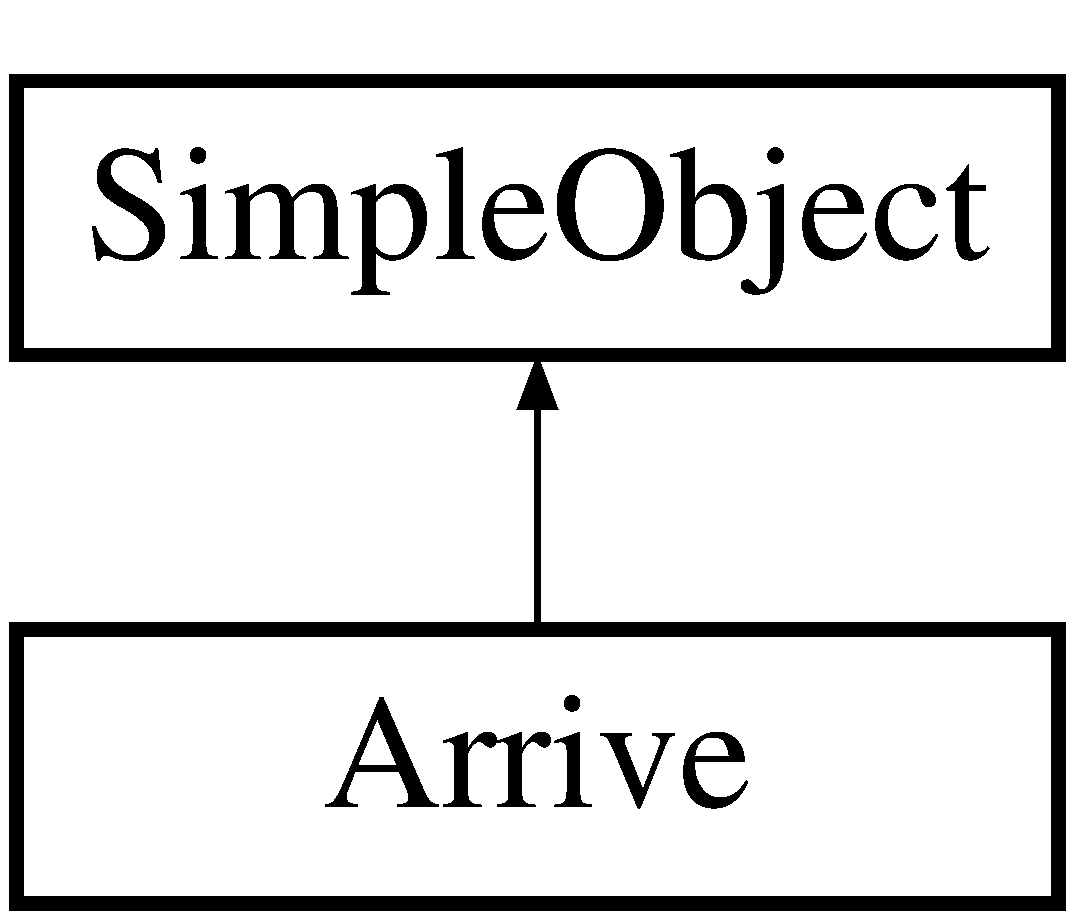
\includegraphics[height=2.000000cm]{classArrive}
\end{center}
\end{figure}
\subsection*{Fonctions membres publiques}
\begin{DoxyCompactItemize}
\item 
bool \hyperlink{classArrive_ab0484a9338e3774c5fa824153b1470e2}{set\-Position} (int8\-\_\-t x, int8\-\_\-t y) override
\item 
pair$<$ int8\-\_\-t, int8\-\_\-t $>$ \hyperlink{classArrive_abe91e4a5bcf15ff987ab58c05b6bb537}{get\-Position} () override
\item 
string \hyperlink{classArrive_af97f0e7e0624cce7ca09d52675e19872}{to\-String} () override
\item 
\hyperlink{classArrive_a65994a8b59dad5bd69480fb85c07d72b}{$\sim$\-Arrive} ()
\end{DoxyCompactItemize}
\subsection*{Fonctions membres publiques statiques}
\begin{DoxyCompactItemize}
\item 
static \hyperlink{classArrive}{Arrive} $\ast$ \hyperlink{classArrive_a0614a2400b23b0ec86294d1776067df2}{get\-Instance} ()
\end{DoxyCompactItemize}
\subsection*{Fonctions membres privées}
\begin{DoxyCompactItemize}
\item 
\hyperlink{classArrive_a55dd55358bedefc3f0c82dd83fdfec79}{Arrive} ()
\end{DoxyCompactItemize}
\subsection*{Attributs privés}
\begin{DoxyCompactItemize}
\item 
pair$<$ int8\-\_\-t, int8\-\_\-t $>$ $\ast$ \hyperlink{classArrive_aa47d57970460b95cfbcdbe62e22dfac7}{position}
\end{DoxyCompactItemize}
\subsection*{Attributs privés statiques}
\begin{DoxyCompactItemize}
\item 
static \hyperlink{classArrive}{Arrive} $\ast$ \hyperlink{classArrive_a92c9b9165c713ff9151d8720660837ef}{instance} = nullptr
\end{DoxyCompactItemize}


\subsection{Documentation des constructeurs et destructeur}
\hypertarget{classArrive_a65994a8b59dad5bd69480fb85c07d72b}{\index{Arrive@{Arrive}!$\sim$\-Arrive@{$\sim$\-Arrive}}
\index{$\sim$\-Arrive@{$\sim$\-Arrive}!Arrive@{Arrive}}
\subsubsection[{$\sim$\-Arrive}]{\setlength{\rightskip}{0pt plus 5cm}Arrive\-::$\sim$\-Arrive (
\begin{DoxyParamCaption}
{}
\end{DoxyParamCaption}
)\hspace{0.3cm}{\ttfamily [inline]}}}\label{classArrive_a65994a8b59dad5bd69480fb85c07d72b}

\begin{DoxyCode}
38              \{
39         \textcolor{keyword}{delete} \hyperlink{classArrive_aa47d57970460b95cfbcdbe62e22dfac7}{position};
40         \hyperlink{classArrive_aa47d57970460b95cfbcdbe62e22dfac7}{position} = \textcolor{keyword}{nullptr};
41         \textcolor{keyword}{delete} \hyperlink{classArrive_a92c9b9165c713ff9151d8720660837ef}{instance};
42         \hyperlink{classArrive_a92c9b9165c713ff9151d8720660837ef}{instance}=\textcolor{keyword}{nullptr};
43     \}
\end{DoxyCode}
\hypertarget{classArrive_a55dd55358bedefc3f0c82dd83fdfec79}{\index{Arrive@{Arrive}!Arrive@{Arrive}}
\index{Arrive@{Arrive}!Arrive@{Arrive}}
\subsubsection[{Arrive}]{\setlength{\rightskip}{0pt plus 5cm}Arrive\-::\-Arrive (
\begin{DoxyParamCaption}
{}
\end{DoxyParamCaption}
)\hspace{0.3cm}{\ttfamily [inline]}, {\ttfamily [private]}}}\label{classArrive_a55dd55358bedefc3f0c82dd83fdfec79}


Référencé par get\-Instance().


\begin{DoxyCode}
48             \{
49         \hyperlink{classArrive_aa47d57970460b95cfbcdbe62e22dfac7}{position} = \textcolor{keyword}{new} pair<int8\_t, int8\_t>();
50         \hyperlink{classArrive_aa47d57970460b95cfbcdbe62e22dfac7}{position}->first = -1;
51         \hyperlink{classArrive_aa47d57970460b95cfbcdbe62e22dfac7}{position}->second = -1;
52     \}
\end{DoxyCode}


\subsection{Documentation des fonctions membres}
\hypertarget{classArrive_a0614a2400b23b0ec86294d1776067df2}{\index{Arrive@{Arrive}!get\-Instance@{get\-Instance}}
\index{get\-Instance@{get\-Instance}!Arrive@{Arrive}}
\subsubsection[{get\-Instance}]{\setlength{\rightskip}{0pt plus 5cm}{\bf Arrive} $\ast$ Arrive\-::get\-Instance (
\begin{DoxyParamCaption}
{}
\end{DoxyParamCaption}
)\hspace{0.3cm}{\ttfamily [static]}}}\label{classArrive_a0614a2400b23b0ec86294d1776067df2}


Références Arrive(), et instance.



Référencé par Manager\-::\-Manager().


\begin{DoxyCode}
9                             \{
10     \textcolor{keywordflow}{if}(\hyperlink{classArrive_a92c9b9165c713ff9151d8720660837ef}{instance} == \textcolor{keyword}{nullptr})\{
11         \hyperlink{classArrive_a92c9b9165c713ff9151d8720660837ef}{instance} = \textcolor{keyword}{new} \hyperlink{classArrive_a55dd55358bedefc3f0c82dd83fdfec79}{Arrive}();
12     \}
13     \textcolor{keywordflow}{return} \hyperlink{classArrive_a92c9b9165c713ff9151d8720660837ef}{instance};
14 \}
\end{DoxyCode}
\hypertarget{classArrive_abe91e4a5bcf15ff987ab58c05b6bb537}{\index{Arrive@{Arrive}!get\-Position@{get\-Position}}
\index{get\-Position@{get\-Position}!Arrive@{Arrive}}
\subsubsection[{get\-Position}]{\setlength{\rightskip}{0pt plus 5cm}pair$<$int8\-\_\-t, int8\-\_\-t$>$ Arrive\-::get\-Position (
\begin{DoxyParamCaption}
{}
\end{DoxyParamCaption}
)\hspace{0.3cm}{\ttfamily [inline]}, {\ttfamily [override]}, {\ttfamily [virtual]}}}\label{classArrive_abe91e4a5bcf15ff987ab58c05b6bb537}


Implémente \hyperlink{classSimpleObject_ae417f1a285ceab5a04130aba01bac856}{Simple\-Object}.



Référencé par Core\-::draw\-Debug(), Core\-::pathfinding(), to\-String(), unitest\-\_\-pathfinding(), et Manager\-::update().


\begin{DoxyCode}
34                                                \{
35         \textcolor{keywordflow}{return} *\hyperlink{classArrive_aa47d57970460b95cfbcdbe62e22dfac7}{position};
36     \}
\end{DoxyCode}
\hypertarget{classArrive_ab0484a9338e3774c5fa824153b1470e2}{\index{Arrive@{Arrive}!set\-Position@{set\-Position}}
\index{set\-Position@{set\-Position}!Arrive@{Arrive}}
\subsubsection[{set\-Position}]{\setlength{\rightskip}{0pt plus 5cm}bool Arrive\-::set\-Position (
\begin{DoxyParamCaption}
\item[{int8\-\_\-t}]{x, }
\item[{int8\-\_\-t}]{y}
\end{DoxyParamCaption}
)\hspace{0.3cm}{\ttfamily [inline]}, {\ttfamily [override]}, {\ttfamily [virtual]}}}\label{classArrive_ab0484a9338e3774c5fa824153b1470e2}


Implémente \hyperlink{classSimpleObject_ae9ea1f7ffe6d4aaf18f24e937e6b60ab}{Simple\-Object}.



Référencé par Core\-::block\-Processing(), Manager\-::reset(), et unitest\-\_\-pathfinding().


\begin{DoxyCode}
29                                                  \{
30         \hyperlink{classArrive_aa47d57970460b95cfbcdbe62e22dfac7}{position}->first = x;
31         \hyperlink{classArrive_aa47d57970460b95cfbcdbe62e22dfac7}{position}->second = y;
32         \textcolor{keywordflow}{return} (\hyperlink{classArrive_aa47d57970460b95cfbcdbe62e22dfac7}{position}->first == x && \hyperlink{classArrive_aa47d57970460b95cfbcdbe62e22dfac7}{position}->second == y);
33     \}
\end{DoxyCode}
\hypertarget{classArrive_af97f0e7e0624cce7ca09d52675e19872}{\index{Arrive@{Arrive}!to\-String@{to\-String}}
\index{to\-String@{to\-String}!Arrive@{Arrive}}
\subsubsection[{to\-String}]{\setlength{\rightskip}{0pt plus 5cm}std\-::string Arrive\-::to\-String (
\begin{DoxyParamCaption}
{}
\end{DoxyParamCaption}
)\hspace{0.3cm}{\ttfamily [override]}, {\ttfamily [virtual]}}}\label{classArrive_af97f0e7e0624cce7ca09d52675e19872}


Implémente \hyperlink{classSimpleObject_aedf0ddcc119ab40623b5b69badc9531a}{Simple\-Object}.



Références get\-Position().



Référencé par Manager\-::to\-String().


\begin{DoxyCode}
16                           \{
17     stringstream buf;
18     buf<<\textcolor{stringliteral}{"\(\backslash\)"Arrive\(\backslash\)": \{ \(\backslash\)"X\(\backslash\)": "}<<(int)\hyperlink{classArrive_abe91e4a5bcf15ff987ab58c05b6bb537}{getPosition}().first<<\textcolor{stringliteral}{", \(\backslash\)"Y\(\backslash\)": "}<<(int)
      \hyperlink{classArrive_abe91e4a5bcf15ff987ab58c05b6bb537}{getPosition}().second<<\textcolor{stringliteral}{" \}"};
19     \textcolor{keywordflow}{return} buf.str();
20 \}\end{DoxyCode}


\subsection{Documentation des données membres}
\hypertarget{classArrive_a92c9b9165c713ff9151d8720660837ef}{\index{Arrive@{Arrive}!instance@{instance}}
\index{instance@{instance}!Arrive@{Arrive}}
\subsubsection[{instance}]{\setlength{\rightskip}{0pt plus 5cm}{\bf Arrive} $\ast$ Arrive\-::instance = nullptr\hspace{0.3cm}{\ttfamily [static]}, {\ttfamily [private]}}}\label{classArrive_a92c9b9165c713ff9151d8720660837ef}


Référencé par get\-Instance().

\hypertarget{classArrive_aa47d57970460b95cfbcdbe62e22dfac7}{\index{Arrive@{Arrive}!position@{position}}
\index{position@{position}!Arrive@{Arrive}}
\subsubsection[{position}]{\setlength{\rightskip}{0pt plus 5cm}pair$<$int8\-\_\-t, int8\-\_\-t$>$$\ast$ Arrive\-::position\hspace{0.3cm}{\ttfamily [private]}}}\label{classArrive_aa47d57970460b95cfbcdbe62e22dfac7}


La documentation de cette classe a été générée à partir des fichiers suivants \-:\begin{DoxyCompactItemize}
\item 
headers/manager/\hyperlink{arrive_8h}{arrive.\-h}\item 
sources/\hyperlink{arrive_8cpp}{arrive.\-cpp}\end{DoxyCompactItemize}

\hypertarget{classBloc}{\section{Référence de la classe Bloc}
\label{classBloc}\index{Bloc@{Bloc}}
}


{\ttfamily \#include $<$bloc.\-h$>$}

Graphe d'héritage de Bloc\-:\begin{figure}[H]
\begin{center}
\leavevmode
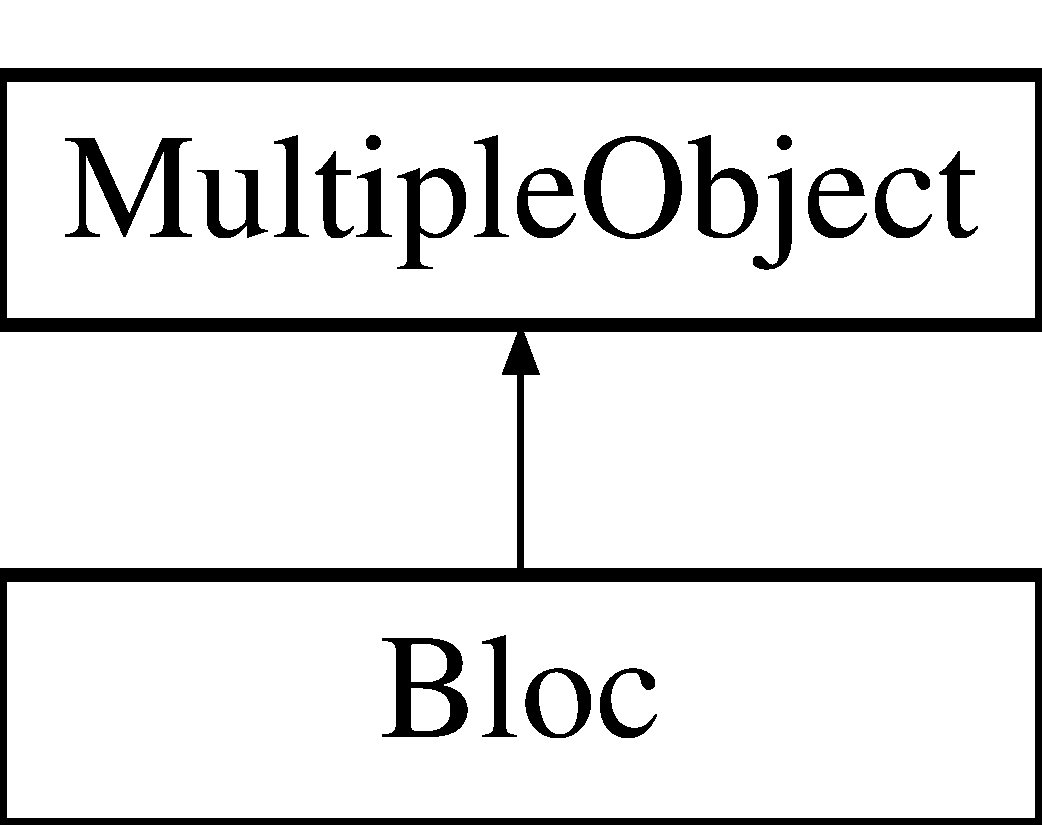
\includegraphics[height=2.000000cm]{classBloc}
\end{center}
\end{figure}
\subsection*{Fonctions membres publiques}
\begin{DoxyCompactItemize}
\item 
bool \hyperlink{classBloc_a02db4c95699ce40e8ad671ef759ebdb7}{add} (int8\-\_\-t x, int8\-\_\-t y) override
\item 
bool \hyperlink{classBloc_a259248faed302444ba5424cdf6178681}{remove} (int8\-\_\-t x, int8\-\_\-t y) override
\item 
bool \hyperlink{classBloc_a8e62a350fb01ea58c9a8bb4deb08639e}{set} (std\-::vector$<$ std\-::pair$<$ int8\-\_\-t, int8\-\_\-t $>$$>$ list)
\item 
bool \hyperlink{classBloc_a03799c83e18411ab4ae4bf3e03aec975}{has} (int8\-\_\-t x, int8\-\_\-t y) override
\item 
bool \hyperlink{classBloc_afa48be18bb2cd4e3240f4a165abef1c8}{clear} () override
\item 
string \hyperlink{classBloc_a040af8a2aefc1acaa0e2d9bfc5943fa3}{to\-String} () override
\item 
\hyperlink{classBloc_a1f40a68b1acb741fc91e07bbaa61dc22}{$\sim$\-Bloc} ()
\end{DoxyCompactItemize}
\subsection*{Fonctions membres publiques statiques}
\begin{DoxyCompactItemize}
\item 
static \hyperlink{classBloc}{Bloc} $\ast$ \hyperlink{classBloc_af357c5eeff01b5b41d983b1e42f5c115}{get\-Instance} ()
\end{DoxyCompactItemize}
\subsection*{Attributs publics}
\begin{DoxyCompactItemize}
\item 
vector$<$ pair$<$ int8\-\_\-t, int8\-\_\-t $>$ $>$ $\ast$ \hyperlink{classBloc_a51ad89062b91675830e0285f992f3210}{list\-\_\-bloc}
\end{DoxyCompactItemize}
\subsection*{Fonctions membres privées}
\begin{DoxyCompactItemize}
\item 
\hyperlink{classBloc_ae3ac5cbad6363c4ab56262a94d0b982e}{Bloc} ()
\end{DoxyCompactItemize}
\subsection*{Attributs privés statiques}
\begin{DoxyCompactItemize}
\item 
static \hyperlink{classBloc}{Bloc} $\ast$ \hyperlink{classBloc_a39298425a48bcca70e70464f51193507}{instance} = nullptr
\end{DoxyCompactItemize}


\subsection{Documentation des constructeurs et destructeur}
\hypertarget{classBloc_a1f40a68b1acb741fc91e07bbaa61dc22}{\index{Bloc@{Bloc}!$\sim$\-Bloc@{$\sim$\-Bloc}}
\index{$\sim$\-Bloc@{$\sim$\-Bloc}!Bloc@{Bloc}}
\subsubsection[{$\sim$\-Bloc}]{\setlength{\rightskip}{0pt plus 5cm}Bloc\-::$\sim$\-Bloc (
\begin{DoxyParamCaption}
{}
\end{DoxyParamCaption}
)\hspace{0.3cm}{\ttfamily [inline]}}}\label{classBloc_a1f40a68b1acb741fc91e07bbaa61dc22}

\begin{DoxyCode}
48            \{
49         \textcolor{keyword}{delete} []\hyperlink{classBloc_a51ad89062b91675830e0285f992f3210}{list\_bloc};
50         \hyperlink{classBloc_a51ad89062b91675830e0285f992f3210}{list\_bloc} = \textcolor{keyword}{nullptr};
51         \textcolor{keyword}{delete} \hyperlink{classBloc_a39298425a48bcca70e70464f51193507}{instance};
52         \hyperlink{classBloc_a39298425a48bcca70e70464f51193507}{instance} = \textcolor{keyword}{nullptr};
53     \}
\end{DoxyCode}
\hypertarget{classBloc_ae3ac5cbad6363c4ab56262a94d0b982e}{\index{Bloc@{Bloc}!Bloc@{Bloc}}
\index{Bloc@{Bloc}!Bloc@{Bloc}}
\subsubsection[{Bloc}]{\setlength{\rightskip}{0pt plus 5cm}Bloc\-::\-Bloc (
\begin{DoxyParamCaption}
{}
\end{DoxyParamCaption}
)\hspace{0.3cm}{\ttfamily [inline]}, {\ttfamily [private]}}}\label{classBloc_ae3ac5cbad6363c4ab56262a94d0b982e}


Références M\-A\-X\-\_\-\-B\-L\-O\-C\-\_\-\-S\-C\-E\-N\-E.



Référencé par get\-Instance().


\begin{DoxyCode}
57           \{
58         \hyperlink{classBloc_a51ad89062b91675830e0285f992f3210}{list\_bloc} = \textcolor{keyword}{new} vector<pair<int8\_t, int8\_t>>();
59         \hyperlink{classBloc_a51ad89062b91675830e0285f992f3210}{list\_bloc}->reserve(\hyperlink{definition_8h_a9ddbbce2fd669544c295551b85ca01ff}{MAX\_BLOC\_SCENE});
60     \}
\end{DoxyCode}


\subsection{Documentation des fonctions membres}
\hypertarget{classBloc_a02db4c95699ce40e8ad671ef759ebdb7}{\index{Bloc@{Bloc}!add@{add}}
\index{add@{add}!Bloc@{Bloc}}
\subsubsection[{add}]{\setlength{\rightskip}{0pt plus 5cm}bool Bloc\-::add (
\begin{DoxyParamCaption}
\item[{int8\-\_\-t}]{x, }
\item[{int8\-\_\-t}]{y}
\end{DoxyParamCaption}
)\hspace{0.3cm}{\ttfamily [override]}, {\ttfamily [virtual]}}}\label{classBloc_a02db4c95699ce40e8ad671ef759ebdb7}


Implémente \hyperlink{classMultipleObject_aa5e743143bdedeb901c8e234162b3db1}{Multiple\-Object}.



Références list\-\_\-bloc.



Référencé par Core\-::block\-Processing(), et unitest\-\_\-pathfinding().


\begin{DoxyCode}
16                                 \{
17     \hyperlink{classBloc_a51ad89062b91675830e0285f992f3210}{list\_bloc}->push\_back(std::make\_pair(x,y));
18     \textcolor{keywordflow}{return} std::find(\hyperlink{classBloc_a51ad89062b91675830e0285f992f3210}{list\_bloc}->begin(), \hyperlink{classBloc_a51ad89062b91675830e0285f992f3210}{list\_bloc}->end(), std::make\_pair(x,y)) != 
      \hyperlink{classBloc_a51ad89062b91675830e0285f992f3210}{list\_bloc}->end();
19 \}
\end{DoxyCode}
\hypertarget{classBloc_afa48be18bb2cd4e3240f4a165abef1c8}{\index{Bloc@{Bloc}!clear@{clear}}
\index{clear@{clear}!Bloc@{Bloc}}
\subsubsection[{clear}]{\setlength{\rightskip}{0pt plus 5cm}bool Bloc\-::clear (
\begin{DoxyParamCaption}
{}
\end{DoxyParamCaption}
)\hspace{0.3cm}{\ttfamily [inline]}, {\ttfamily [override]}, {\ttfamily [virtual]}}}\label{classBloc_afa48be18bb2cd4e3240f4a165abef1c8}


Implémente \hyperlink{classMultipleObject_a980acdfb99e25ec0d5e61396f60517c3}{Multiple\-Object}.



Référencé par Manager\-::reset().


\begin{DoxyCode}
43                          \{
44         \hyperlink{classBloc_a51ad89062b91675830e0285f992f3210}{list\_bloc}->clear();
45         \textcolor{keywordflow}{return} \hyperlink{classBloc_a51ad89062b91675830e0285f992f3210}{list\_bloc}->size() == 0;
46     \}
\end{DoxyCode}
\hypertarget{classBloc_af357c5eeff01b5b41d983b1e42f5c115}{\index{Bloc@{Bloc}!get\-Instance@{get\-Instance}}
\index{get\-Instance@{get\-Instance}!Bloc@{Bloc}}
\subsubsection[{get\-Instance}]{\setlength{\rightskip}{0pt plus 5cm}{\bf Bloc} $\ast$ Bloc\-::get\-Instance (
\begin{DoxyParamCaption}
{}
\end{DoxyParamCaption}
)\hspace{0.3cm}{\ttfamily [static]}}}\label{classBloc_af357c5eeff01b5b41d983b1e42f5c115}


Références Bloc(), et instance.



Référencé par Manager\-::\-Manager(), et unitest\-\_\-pathfinding().


\begin{DoxyCode}
9                         \{
10     \textcolor{keywordflow}{if}(\hyperlink{classBloc_a39298425a48bcca70e70464f51193507}{instance} == \textcolor{keyword}{nullptr})\{
11         \hyperlink{classBloc_a39298425a48bcca70e70464f51193507}{instance} = \textcolor{keyword}{new} \hyperlink{classBloc_ae3ac5cbad6363c4ab56262a94d0b982e}{Bloc}();
12     \}
13     \textcolor{keywordflow}{return} \hyperlink{classBloc_a39298425a48bcca70e70464f51193507}{instance};
14 \}
\end{DoxyCode}
\hypertarget{classBloc_a03799c83e18411ab4ae4bf3e03aec975}{\index{Bloc@{Bloc}!has@{has}}
\index{has@{has}!Bloc@{Bloc}}
\subsubsection[{has}]{\setlength{\rightskip}{0pt plus 5cm}bool Bloc\-::has (
\begin{DoxyParamCaption}
\item[{int8\-\_\-t}]{x, }
\item[{int8\-\_\-t}]{y}
\end{DoxyParamCaption}
)\hspace{0.3cm}{\ttfamily [override]}, {\ttfamily [virtual]}}}\label{classBloc_a03799c83e18411ab4ae4bf3e03aec975}


Implémente \hyperlink{classMultipleObject_a1703b0c461708fbb6985e87624f4b17b}{Multiple\-Object}.



Références list\-\_\-bloc.



Référencé par remove(), et unitest\-\_\-pathfinding().


\begin{DoxyCode}
29                                 \{
30     \textcolor{keywordflow}{return} std::find(\hyperlink{classBloc_a51ad89062b91675830e0285f992f3210}{list\_bloc}->begin(), \hyperlink{classBloc_a51ad89062b91675830e0285f992f3210}{list\_bloc}->end(), std::make\_pair(x,y)) != 
      \hyperlink{classBloc_a51ad89062b91675830e0285f992f3210}{list\_bloc}->end();
31 \}
\end{DoxyCode}
\hypertarget{classBloc_a259248faed302444ba5424cdf6178681}{\index{Bloc@{Bloc}!remove@{remove}}
\index{remove@{remove}!Bloc@{Bloc}}
\subsubsection[{remove}]{\setlength{\rightskip}{0pt plus 5cm}bool Bloc\-::remove (
\begin{DoxyParamCaption}
\item[{int8\-\_\-t}]{x, }
\item[{int8\-\_\-t}]{y}
\end{DoxyParamCaption}
)\hspace{0.3cm}{\ttfamily [override]}, {\ttfamily [virtual]}}}\label{classBloc_a259248faed302444ba5424cdf6178681}


Implémente \hyperlink{classMultipleObject_ad57dd5fec65953bbce399afdca475a4c}{Multiple\-Object}.



Références has(), et list\-\_\-bloc.



Référencé par unitest\-\_\-pathfinding().


\begin{DoxyCode}
21                                    \{
22     \textcolor{keywordflow}{if}(\hyperlink{classBloc_a03799c83e18411ab4ae4bf3e03aec975}{has}(x,y))\{
23         \hyperlink{classBloc_a51ad89062b91675830e0285f992f3210}{list\_bloc}->erase(std::remove(\hyperlink{classBloc_a51ad89062b91675830e0285f992f3210}{list\_bloc}->begin(), 
      \hyperlink{classBloc_a51ad89062b91675830e0285f992f3210}{list\_bloc}->end(), std::make\_pair(x,y)), \hyperlink{classBloc_a51ad89062b91675830e0285f992f3210}{list\_bloc}->end());
24         \textcolor{keywordflow}{return} !\hyperlink{classBloc_a03799c83e18411ab4ae4bf3e03aec975}{has}(x,y);
25     \}
26         \textcolor{keywordflow}{return} \textcolor{keyword}{true}; \textcolor{comment}{//default true if isn't in table.}
27 \}
\end{DoxyCode}
\hypertarget{classBloc_a8e62a350fb01ea58c9a8bb4deb08639e}{\index{Bloc@{Bloc}!set@{set}}
\index{set@{set}!Bloc@{Bloc}}
\subsubsection[{set}]{\setlength{\rightskip}{0pt plus 5cm}bool Bloc\-::set (
\begin{DoxyParamCaption}
\item[{std\-::vector$<$ std\-::pair$<$ int8\-\_\-t, int8\-\_\-t $>$$>$}]{list}
\end{DoxyParamCaption}
)\hspace{0.3cm}{\ttfamily [inline]}}}\label{classBloc_a8e62a350fb01ea58c9a8bb4deb08639e}

\begin{DoxyCode}
34                                                      \{
35         \textcolor{keywordtype}{bool} ret = \hyperlink{classBloc_afa48be18bb2cd4e3240f4a165abef1c8}{clear}();
36         \textcolor{keywordflow}{for}(int8\_t i=0; i<list.size(); ++i)
37             \hyperlink{classBloc_a51ad89062b91675830e0285f992f3210}{list\_bloc}->push\_back(list[i]);
38         \textcolor{keywordflow}{if}(\hyperlink{classBloc_a51ad89062b91675830e0285f992f3210}{list\_bloc}->size() > 0)
39             ret = \textcolor{keyword}{false};
40         \textcolor{keywordflow}{return} ret;
41     \}    
\end{DoxyCode}
\hypertarget{classBloc_a040af8a2aefc1acaa0e2d9bfc5943fa3}{\index{Bloc@{Bloc}!to\-String@{to\-String}}
\index{to\-String@{to\-String}!Bloc@{Bloc}}
\subsubsection[{to\-String}]{\setlength{\rightskip}{0pt plus 5cm}string Bloc\-::to\-String (
\begin{DoxyParamCaption}
{}
\end{DoxyParamCaption}
)\hspace{0.3cm}{\ttfamily [override]}, {\ttfamily [virtual]}}}\label{classBloc_a040af8a2aefc1acaa0e2d9bfc5943fa3}


Implémente \hyperlink{classMultipleObject_a5439a2ac4cc86c759ef1df8f6059947a}{Multiple\-Object}.



Références list\-\_\-bloc.



Référencé par Manager\-::to\-String(), et unitest\-\_\-pathfinding().


\begin{DoxyCode}
33                      \{
34     int16\_t size = \hyperlink{classBloc_a51ad89062b91675830e0285f992f3210}{list\_bloc}->size();
35     stringstream value;
36     value << \textcolor{stringliteral}{""};
37     int16\_t i =0;
38     std::for\_each(\hyperlink{classBloc_a51ad89062b91675830e0285f992f3210}{list\_bloc}->begin(), \hyperlink{classBloc_a51ad89062b91675830e0285f992f3210}{list\_bloc}->end(), [&](std::pair<int8\_t, int8\_t> \_b)
      \{
39         value << \textcolor{stringliteral}{"\(\backslash\)""}<<i<<\textcolor{stringliteral}{"\(\backslash\)": \(\backslash\)""}<<(int)\_b.first<< \textcolor{stringliteral}{","} <<(\textcolor{keywordtype}{int})\_b.second<<\textcolor{stringliteral}{"\(\backslash\)", "};
40         ++i;
41     \});
42     stringstream buf;
43     buf <<\textcolor{stringliteral}{" \(\backslash\)"Bloc\(\backslash\)": \{ \(\backslash\)"Number\(\backslash\)": "}<<size<<\textcolor{stringliteral}{", \(\backslash\)"Position\(\backslash\)": \{"}<<value.str().substr(0, value.str().size()-
      2)<<\textcolor{stringliteral}{"\} \}"};
44     \textcolor{keywordflow}{return} buf.str();
45 \}
\end{DoxyCode}


\subsection{Documentation des données membres}
\hypertarget{classBloc_a39298425a48bcca70e70464f51193507}{\index{Bloc@{Bloc}!instance@{instance}}
\index{instance@{instance}!Bloc@{Bloc}}
\subsubsection[{instance}]{\setlength{\rightskip}{0pt plus 5cm}{\bf Bloc} $\ast$ Bloc\-::instance = nullptr\hspace{0.3cm}{\ttfamily [static]}, {\ttfamily [private]}}}\label{classBloc_a39298425a48bcca70e70464f51193507}


Référencé par get\-Instance().

\hypertarget{classBloc_a51ad89062b91675830e0285f992f3210}{\index{Bloc@{Bloc}!list\-\_\-bloc@{list\-\_\-bloc}}
\index{list\-\_\-bloc@{list\-\_\-bloc}!Bloc@{Bloc}}
\subsubsection[{list\-\_\-bloc}]{\setlength{\rightskip}{0pt plus 5cm}vector$<$pair$<$int8\-\_\-t,int8\-\_\-t$>$ $>$$\ast$ Bloc\-::list\-\_\-bloc}}\label{classBloc_a51ad89062b91675830e0285f992f3210}


Référencé par add(), Core\-::draw\-Debug(), has(), remove(), to\-String(), et Manager\-::update().



La documentation de cette classe a été générée à partir des fichiers suivants \-:\begin{DoxyCompactItemize}
\item 
headers/manager/\hyperlink{bloc_8h}{bloc.\-h}\item 
sources/\hyperlink{bloc_8cpp}{bloc.\-cpp}\end{DoxyCompactItemize}

\hypertarget{classCar}{\section{Référence de la classe Car}
\label{classCar}\index{Car@{Car}}
}


{\ttfamily \#include $<$car.\-h$>$}

Graphe d'héritage de Car\-:\begin{figure}[H]
\begin{center}
\leavevmode
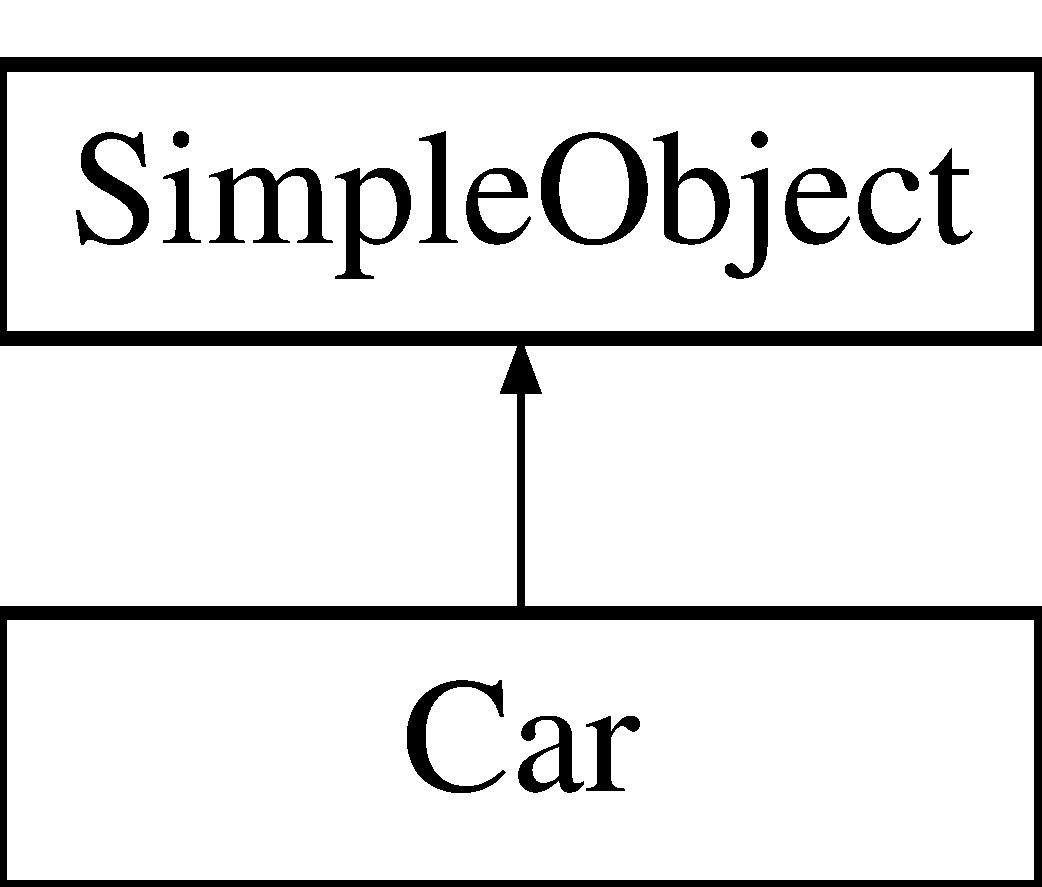
\includegraphics[height=2.000000cm]{classCar}
\end{center}
\end{figure}
\subsection*{Fonctions membres publiques}
\begin{DoxyCompactItemize}
\item 
void \hyperlink{classCar_a2d3353932e4028eef864813b8c65583b}{send\-Command} ()
\item 
bool \hyperlink{classCar_a97e3c5de8eb65659ef520de6591f814d}{set\-Position} (int8\-\_\-t x, int8\-\_\-t y) override
\item 
pair$<$ int8\-\_\-t, int8\-\_\-t $>$ \hyperlink{classCar_a20dd521474ee36b144bde58e3359eed6}{get\-Position} () override
\item 
string \hyperlink{classCar_afb39c5a80ff1977ee13cb1e5cdf2fecd}{to\-String} () override
\item 
\hyperlink{classCar_a5933bb06e96b159fe339a128abda888a}{$\sim$\-Car} ()
\end{DoxyCompactItemize}
\subsection*{Fonctions membres publiques statiques}
\begin{DoxyCompactItemize}
\item 
static \hyperlink{classCar}{Car} $\ast$ \hyperlink{classCar_a40cbec40dad9ddda76c277da17f23528}{get\-Instance} ()
\end{DoxyCompactItemize}
\subsection*{Fonctions membres privées}
\begin{DoxyCompactItemize}
\item 
\hyperlink{classCar_a1c803f7c5038d3e31b368b0d0a35493c}{Car} ()
\end{DoxyCompactItemize}
\subsection*{Attributs privés}
\begin{DoxyCompactItemize}
\item 
pair$<$ int8\-\_\-t, int8\-\_\-t $>$ $\ast$ \hyperlink{classCar_a43e9c00e78af10fc998624a811e014df}{position}
\end{DoxyCompactItemize}
\subsection*{Attributs privés statiques}
\begin{DoxyCompactItemize}
\item 
static \hyperlink{classCar}{Car} $\ast$ \hyperlink{classCar_a4e8c86d0fa20de2108d524056cf4bc85}{instance} = nullptr
\end{DoxyCompactItemize}


\subsection{Documentation des constructeurs et destructeur}
\hypertarget{classCar_a5933bb06e96b159fe339a128abda888a}{\index{Car@{Car}!$\sim$\-Car@{$\sim$\-Car}}
\index{$\sim$\-Car@{$\sim$\-Car}!Car@{Car}}
\subsubsection[{$\sim$\-Car}]{\setlength{\rightskip}{0pt plus 5cm}Car\-::$\sim$\-Car (
\begin{DoxyParamCaption}
{}
\end{DoxyParamCaption}
)\hspace{0.3cm}{\ttfamily [inline]}}}\label{classCar_a5933bb06e96b159fe339a128abda888a}

\begin{DoxyCode}
29           \{
30         \textcolor{keyword}{delete} \hyperlink{classCar_a43e9c00e78af10fc998624a811e014df}{position};
31         \hyperlink{classCar_a43e9c00e78af10fc998624a811e014df}{position} = \textcolor{keyword}{nullptr};
32         \textcolor{keyword}{delete} \hyperlink{classCar_a4e8c86d0fa20de2108d524056cf4bc85}{instance};
33         \hyperlink{classCar_a4e8c86d0fa20de2108d524056cf4bc85}{instance} = \textcolor{keyword}{nullptr};
34     \}
\end{DoxyCode}
\hypertarget{classCar_a1c803f7c5038d3e31b368b0d0a35493c}{\index{Car@{Car}!Car@{Car}}
\index{Car@{Car}!Car@{Car}}
\subsubsection[{Car}]{\setlength{\rightskip}{0pt plus 5cm}Car\-::\-Car (
\begin{DoxyParamCaption}
{}
\end{DoxyParamCaption}
)\hspace{0.3cm}{\ttfamily [inline]}, {\ttfamily [private]}}}\label{classCar_a1c803f7c5038d3e31b368b0d0a35493c}


Référencé par get\-Instance().


\begin{DoxyCode}
38          \{
39         \hyperlink{classCar_a43e9c00e78af10fc998624a811e014df}{position} = \textcolor{keyword}{new} pair<int8\_t, int8\_t>();
40         \hyperlink{classCar_a43e9c00e78af10fc998624a811e014df}{position}->first = -1;
41         \hyperlink{classCar_a43e9c00e78af10fc998624a811e014df}{position}->second = -1;
42     \}
\end{DoxyCode}


\subsection{Documentation des fonctions membres}
\hypertarget{classCar_a40cbec40dad9ddda76c277da17f23528}{\index{Car@{Car}!get\-Instance@{get\-Instance}}
\index{get\-Instance@{get\-Instance}!Car@{Car}}
\subsubsection[{get\-Instance}]{\setlength{\rightskip}{0pt plus 5cm}{\bf Car} $\ast$ Car\-::get\-Instance (
\begin{DoxyParamCaption}
{}
\end{DoxyParamCaption}
)\hspace{0.3cm}{\ttfamily [static]}}}\label{classCar_a40cbec40dad9ddda76c277da17f23528}


Références Car(), et instance.



Référencé par Manager\-::\-Manager(), et unitest\-\_\-pathfinding().


\begin{DoxyCode}
9                       \{
10     \textcolor{keywordflow}{if}(\hyperlink{classCar_a4e8c86d0fa20de2108d524056cf4bc85}{instance} == \textcolor{keyword}{nullptr})\{
11         \hyperlink{classCar_a4e8c86d0fa20de2108d524056cf4bc85}{instance} = \textcolor{keyword}{new} \hyperlink{classCar_a1c803f7c5038d3e31b368b0d0a35493c}{Car}();
12     \}
13     \textcolor{keywordflow}{return} \hyperlink{classCar_a4e8c86d0fa20de2108d524056cf4bc85}{instance};
14 \}
\end{DoxyCode}
\hypertarget{classCar_a20dd521474ee36b144bde58e3359eed6}{\index{Car@{Car}!get\-Position@{get\-Position}}
\index{get\-Position@{get\-Position}!Car@{Car}}
\subsubsection[{get\-Position}]{\setlength{\rightskip}{0pt plus 5cm}pair$<$int8\-\_\-t, int8\-\_\-t$>$ Car\-::get\-Position (
\begin{DoxyParamCaption}
{}
\end{DoxyParamCaption}
)\hspace{0.3cm}{\ttfamily [inline]}, {\ttfamily [override]}, {\ttfamily [virtual]}}}\label{classCar_a20dd521474ee36b144bde58e3359eed6}


Implémente \hyperlink{classSimpleObject_ae417f1a285ceab5a04130aba01bac856}{Simple\-Object}.



Référencé par Serveur\-::\-Accept\-And\-Dispatch(), Core\-::draw\-Debug(), Core\-::pathfinding(), to\-String(), unitest\-\_\-pathfinding(), et Manager\-::update().


\begin{DoxyCode}
25                                                \{
26         \textcolor{keywordflow}{return} *\hyperlink{classCar_a43e9c00e78af10fc998624a811e014df}{position};
27     \}
\end{DoxyCode}
\hypertarget{classCar_a2d3353932e4028eef864813b8c65583b}{\index{Car@{Car}!send\-Command@{send\-Command}}
\index{send\-Command@{send\-Command}!Car@{Car}}
\subsubsection[{send\-Command}]{\setlength{\rightskip}{0pt plus 5cm}void Car\-::send\-Command (
\begin{DoxyParamCaption}
{}
\end{DoxyParamCaption}
)}}\label{classCar_a2d3353932e4028eef864813b8c65583b}

\begin{DoxyCode}
16                      \{
17     \textcolor{comment}{//TODO send command from wifi to Car}
18 \}
\end{DoxyCode}
\hypertarget{classCar_a97e3c5de8eb65659ef520de6591f814d}{\index{Car@{Car}!set\-Position@{set\-Position}}
\index{set\-Position@{set\-Position}!Car@{Car}}
\subsubsection[{set\-Position}]{\setlength{\rightskip}{0pt plus 5cm}bool Car\-::set\-Position (
\begin{DoxyParamCaption}
\item[{int8\-\_\-t}]{x, }
\item[{int8\-\_\-t}]{y}
\end{DoxyParamCaption}
)\hspace{0.3cm}{\ttfamily [inline]}, {\ttfamily [override]}, {\ttfamily [virtual]}}}\label{classCar_a97e3c5de8eb65659ef520de6591f814d}


Implémente \hyperlink{classSimpleObject_ae9ea1f7ffe6d4aaf18f24e937e6b60ab}{Simple\-Object}.



Référencé par Core\-::block\-Processing(), Manager\-::reset(), et unitest\-\_\-pathfinding().


\begin{DoxyCode}
21                                                  \{
22         \hyperlink{classCar_a43e9c00e78af10fc998624a811e014df}{position}->first = x;
23         \hyperlink{classCar_a43e9c00e78af10fc998624a811e014df}{position}->second = y;
24     \}
\end{DoxyCode}
\hypertarget{classCar_afb39c5a80ff1977ee13cb1e5cdf2fecd}{\index{Car@{Car}!to\-String@{to\-String}}
\index{to\-String@{to\-String}!Car@{Car}}
\subsubsection[{to\-String}]{\setlength{\rightskip}{0pt plus 5cm}std\-::string Car\-::to\-String (
\begin{DoxyParamCaption}
{}
\end{DoxyParamCaption}
)\hspace{0.3cm}{\ttfamily [override]}, {\ttfamily [virtual]}}}\label{classCar_afb39c5a80ff1977ee13cb1e5cdf2fecd}


Implémente \hyperlink{classSimpleObject_aedf0ddcc119ab40623b5b69badc9531a}{Simple\-Object}.



Références get\-Position().



Référencé par Manager\-::to\-String().


\begin{DoxyCode}
20                        \{
21     stringstream buf;
22     buf<<\textcolor{stringliteral}{"\(\backslash\)"Voiture\(\backslash\)": \{ \(\backslash\)"X\(\backslash\)": "}<<(int)\hyperlink{classCar_a20dd521474ee36b144bde58e3359eed6}{getPosition}().first<<\textcolor{stringliteral}{", \(\backslash\)"Y\(\backslash\)": "}<<(int)
      \hyperlink{classCar_a20dd521474ee36b144bde58e3359eed6}{getPosition}().second<<\textcolor{stringliteral}{" \}"};
23     \textcolor{keywordflow}{return} buf.str();
24 \}\end{DoxyCode}


\subsection{Documentation des données membres}
\hypertarget{classCar_a4e8c86d0fa20de2108d524056cf4bc85}{\index{Car@{Car}!instance@{instance}}
\index{instance@{instance}!Car@{Car}}
\subsubsection[{instance}]{\setlength{\rightskip}{0pt plus 5cm}{\bf Car} $\ast$ Car\-::instance = nullptr\hspace{0.3cm}{\ttfamily [static]}, {\ttfamily [private]}}}\label{classCar_a4e8c86d0fa20de2108d524056cf4bc85}


Référencé par get\-Instance().

\hypertarget{classCar_a43e9c00e78af10fc998624a811e014df}{\index{Car@{Car}!position@{position}}
\index{position@{position}!Car@{Car}}
\subsubsection[{position}]{\setlength{\rightskip}{0pt plus 5cm}pair$<$int8\-\_\-t, int8\-\_\-t$>$$\ast$ Car\-::position\hspace{0.3cm}{\ttfamily [private]}}}\label{classCar_a43e9c00e78af10fc998624a811e014df}


La documentation de cette classe a été générée à partir des fichiers suivants \-:\begin{DoxyCompactItemize}
\item 
headers/manager/\hyperlink{car_8h}{car.\-h}\item 
sources/\hyperlink{car_8cpp}{car.\-cpp}\end{DoxyCompactItemize}

\hypertarget{classCellule}{\section{Référence de la classe Cellule}
\label{classCellule}\index{Cellule@{Cellule}}
}


{\ttfamily \#include $<$cellule.\-h$>$}

\subsection*{Fonctions membres publiques}
\begin{DoxyCompactItemize}
\item 
\hyperlink{classCellule_af506f7549ec9855560d6e6c5f2988501}{Cellule} (int8\-\_\-t x, int8\-\_\-t y, bool is\-\_\-bloc)
\item 
std\-::pair$<$ int8\-\_\-t, int8\-\_\-t $>$ \hyperlink{classCellule_a50698c84ba5a043a148a594552189427}{get\-Coord} ()
\item 
bool \hyperlink{classCellule_a4f021d3669d6688999f6299372670a60}{is\-Bloc} ()
\item 
\hyperlink{classCellule_a62c79c012c471f8dc74714c3262a696c}{$\sim$\-Cellule} ()
\end{DoxyCompactItemize}
\subsection*{Attributs publics}
\begin{DoxyCompactItemize}
\item 
\hyperlink{classCellule}{Cellule} $\ast$ \hyperlink{classCellule_a3f4117017976fde614e72d38ea10d734}{m\-\_\-parent}
\item 
uint16\-\_\-t \hyperlink{classCellule_af7cb9856701ea3e423f58b09bb7dfdbd}{m\-\_\-\-P}
\item 
bool \hyperlink{classCellule_a9c368e6fb89c5ea1e31b810207eca9ee}{everfind}
\end{DoxyCompactItemize}
\subsection*{Attributs privés}
\begin{DoxyCompactItemize}
\item 
bool \hyperlink{classCellule_adf634a9bd573a298652d70a93f3e5c6e}{m\-\_\-bloc}
\item 
bool \hyperlink{classCellule_abd3eef3d41bf99ca3a1d9edc97aa8282}{is\-\_\-center}
\item 
std\-::pair$<$ int8\-\_\-t, int8\-\_\-t $>$ \hyperlink{classCellule_a9573d226e0df26453a67fb3730794444}{m\-\_\-coord}
\end{DoxyCompactItemize}


\subsection{Documentation des constructeurs et destructeur}
\hypertarget{classCellule_af506f7549ec9855560d6e6c5f2988501}{\index{Cellule@{Cellule}!Cellule@{Cellule}}
\index{Cellule@{Cellule}!Cellule@{Cellule}}
\subsubsection[{Cellule}]{\setlength{\rightskip}{0pt plus 5cm}Cellule\-::\-Cellule (
\begin{DoxyParamCaption}
\item[{int8\-\_\-t}]{x, }
\item[{int8\-\_\-t}]{y, }
\item[{bool}]{is\-\_\-bloc}
\end{DoxyParamCaption}
)\hspace{0.3cm}{\ttfamily [inline]}}}\label{classCellule_af506f7549ec9855560d6e6c5f2988501}


Références everfind, is\-\_\-center, m\-\_\-bloc, m\-\_\-coord, et m\-\_\-\-P.


\begin{DoxyCode}
19                                                  \{
20             \hyperlink{classCellule_a9573d226e0df26453a67fb3730794444}{m\_coord}.first = x;
21             \hyperlink{classCellule_a9573d226e0df26453a67fb3730794444}{m\_coord}.second = y;
22             \hyperlink{classCellule_af7cb9856701ea3e423f58b09bb7dfdbd}{m\_P}= 60000;
23             \hyperlink{classCellule_adf634a9bd573a298652d70a93f3e5c6e}{m\_bloc} = is\_bloc;
24             \hyperlink{classCellule_abd3eef3d41bf99ca3a1d9edc97aa8282}{is\_center}=\textcolor{keyword}{false};
25             \hyperlink{classCellule_a9c368e6fb89c5ea1e31b810207eca9ee}{everfind} = \textcolor{keyword}{false};
26         \}
\end{DoxyCode}
\hypertarget{classCellule_a62c79c012c471f8dc74714c3262a696c}{\index{Cellule@{Cellule}!$\sim$\-Cellule@{$\sim$\-Cellule}}
\index{$\sim$\-Cellule@{$\sim$\-Cellule}!Cellule@{Cellule}}
\subsubsection[{$\sim$\-Cellule}]{\setlength{\rightskip}{0pt plus 5cm}Cellule\-::$\sim$\-Cellule (
\begin{DoxyParamCaption}
{}
\end{DoxyParamCaption}
)\hspace{0.3cm}{\ttfamily [inline]}}}\label{classCellule_a62c79c012c471f8dc74714c3262a696c}


Références m\-\_\-parent.


\begin{DoxyCode}
60                   \{
61             \textcolor{keyword}{delete} \hyperlink{classCellule_a3f4117017976fde614e72d38ea10d734}{m\_parent};
62             \hyperlink{classCellule_a3f4117017976fde614e72d38ea10d734}{m\_parent} = \textcolor{keyword}{nullptr};
63         \}
\end{DoxyCode}


\subsection{Documentation des fonctions membres}
\hypertarget{classCellule_a50698c84ba5a043a148a594552189427}{\index{Cellule@{Cellule}!get\-Coord@{get\-Coord}}
\index{get\-Coord@{get\-Coord}!Cellule@{Cellule}}
\subsubsection[{get\-Coord}]{\setlength{\rightskip}{0pt plus 5cm}std\-::pair$<$int8\-\_\-t, int8\-\_\-t$>$ Cellule\-::get\-Coord (
\begin{DoxyParamCaption}
{}
\end{DoxyParamCaption}
)\hspace{0.3cm}{\ttfamily [inline]}}}\label{classCellule_a50698c84ba5a043a148a594552189427}


Références m\-\_\-coord.



Référencé par Path\-Finding\-::find\-Path(), et Path\-Finding\-::get\-Chemin().


\begin{DoxyCode}
36                                           \{
37             \textcolor{keywordflow}{return} \hyperlink{classCellule_a9573d226e0df26453a67fb3730794444}{m\_coord};
38         \}
\end{DoxyCode}
\hypertarget{classCellule_a4f021d3669d6688999f6299372670a60}{\index{Cellule@{Cellule}!is\-Bloc@{is\-Bloc}}
\index{is\-Bloc@{is\-Bloc}!Cellule@{Cellule}}
\subsubsection[{is\-Bloc}]{\setlength{\rightskip}{0pt plus 5cm}bool Cellule\-::is\-Bloc (
\begin{DoxyParamCaption}
{}
\end{DoxyParamCaption}
)\hspace{0.3cm}{\ttfamily [inline]}}}\label{classCellule_a4f021d3669d6688999f6299372670a60}


Références m\-\_\-bloc.


\begin{DoxyCode}
49                      \{
50             \textcolor{keywordflow}{return} \hyperlink{classCellule_adf634a9bd573a298652d70a93f3e5c6e}{m\_bloc};
51         \}
\end{DoxyCode}


\subsection{Documentation des données membres}
\hypertarget{classCellule_a9c368e6fb89c5ea1e31b810207eca9ee}{\index{Cellule@{Cellule}!everfind@{everfind}}
\index{everfind@{everfind}!Cellule@{Cellule}}
\subsubsection[{everfind}]{\setlength{\rightskip}{0pt plus 5cm}bool Cellule\-::everfind}}\label{classCellule_a9c368e6fb89c5ea1e31b810207eca9ee}


Référencé par Cellule(), Path\-Finding\-::get\-Chemin(), et Path\-Finding\-::\-Path\-Finding().

\hypertarget{classCellule_abd3eef3d41bf99ca3a1d9edc97aa8282}{\index{Cellule@{Cellule}!is\-\_\-center@{is\-\_\-center}}
\index{is\-\_\-center@{is\-\_\-center}!Cellule@{Cellule}}
\subsubsection[{is\-\_\-center}]{\setlength{\rightskip}{0pt plus 5cm}bool Cellule\-::is\-\_\-center\hspace{0.3cm}{\ttfamily [private]}}}\label{classCellule_abd3eef3d41bf99ca3a1d9edc97aa8282}


Référencé par Cellule().

\hypertarget{classCellule_adf634a9bd573a298652d70a93f3e5c6e}{\index{Cellule@{Cellule}!m\-\_\-bloc@{m\-\_\-bloc}}
\index{m\-\_\-bloc@{m\-\_\-bloc}!Cellule@{Cellule}}
\subsubsection[{m\-\_\-bloc}]{\setlength{\rightskip}{0pt plus 5cm}bool Cellule\-::m\-\_\-bloc\hspace{0.3cm}{\ttfamily [private]}}}\label{classCellule_adf634a9bd573a298652d70a93f3e5c6e}


Référencé par Cellule(), et is\-Bloc().

\hypertarget{classCellule_a9573d226e0df26453a67fb3730794444}{\index{Cellule@{Cellule}!m\-\_\-coord@{m\-\_\-coord}}
\index{m\-\_\-coord@{m\-\_\-coord}!Cellule@{Cellule}}
\subsubsection[{m\-\_\-coord}]{\setlength{\rightskip}{0pt plus 5cm}std\-::pair$<$int8\-\_\-t, int8\-\_\-t$>$ Cellule\-::m\-\_\-coord\hspace{0.3cm}{\ttfamily [private]}}}\label{classCellule_a9573d226e0df26453a67fb3730794444}


Référencé par Cellule(), et get\-Coord().

\hypertarget{classCellule_af7cb9856701ea3e423f58b09bb7dfdbd}{\index{Cellule@{Cellule}!m\-\_\-\-P@{m\-\_\-\-P}}
\index{m\-\_\-\-P@{m\-\_\-\-P}!Cellule@{Cellule}}
\subsubsection[{m\-\_\-\-P}]{\setlength{\rightskip}{0pt plus 5cm}uint16\-\_\-t Cellule\-::m\-\_\-\-P}}\label{classCellule_af7cb9856701ea3e423f58b09bb7dfdbd}


Référencé par Cellule(), Path\-Finding\-::find\-Path(), et Path\-Finding\-::\-Path\-Finding().

\hypertarget{classCellule_a3f4117017976fde614e72d38ea10d734}{\index{Cellule@{Cellule}!m\-\_\-parent@{m\-\_\-parent}}
\index{m\-\_\-parent@{m\-\_\-parent}!Cellule@{Cellule}}
\subsubsection[{m\-\_\-parent}]{\setlength{\rightskip}{0pt plus 5cm}{\bf Cellule}$\ast$ Cellule\-::m\-\_\-parent}}\label{classCellule_a3f4117017976fde614e72d38ea10d734}


Référencé par Path\-Finding\-::ever\-Parent(), Path\-Finding\-::find\-Path(), Path\-Finding\-::get\-Chemin(), et $\sim$\-Cellule().



La documentation de cette classe a été générée à partir du fichier suivant \-:\begin{DoxyCompactItemize}
\item 
headers/traitement/\hyperlink{cellule_8h}{cellule.\-h}\end{DoxyCompactItemize}

\hypertarget{classChemin}{\section{Référence de la classe Chemin}
\label{classChemin}\index{Chemin@{Chemin}}
}


{\ttfamily \#include $<$chemin.\-h$>$}

Graphe d'héritage de Chemin\-:\begin{figure}[H]
\begin{center}
\leavevmode
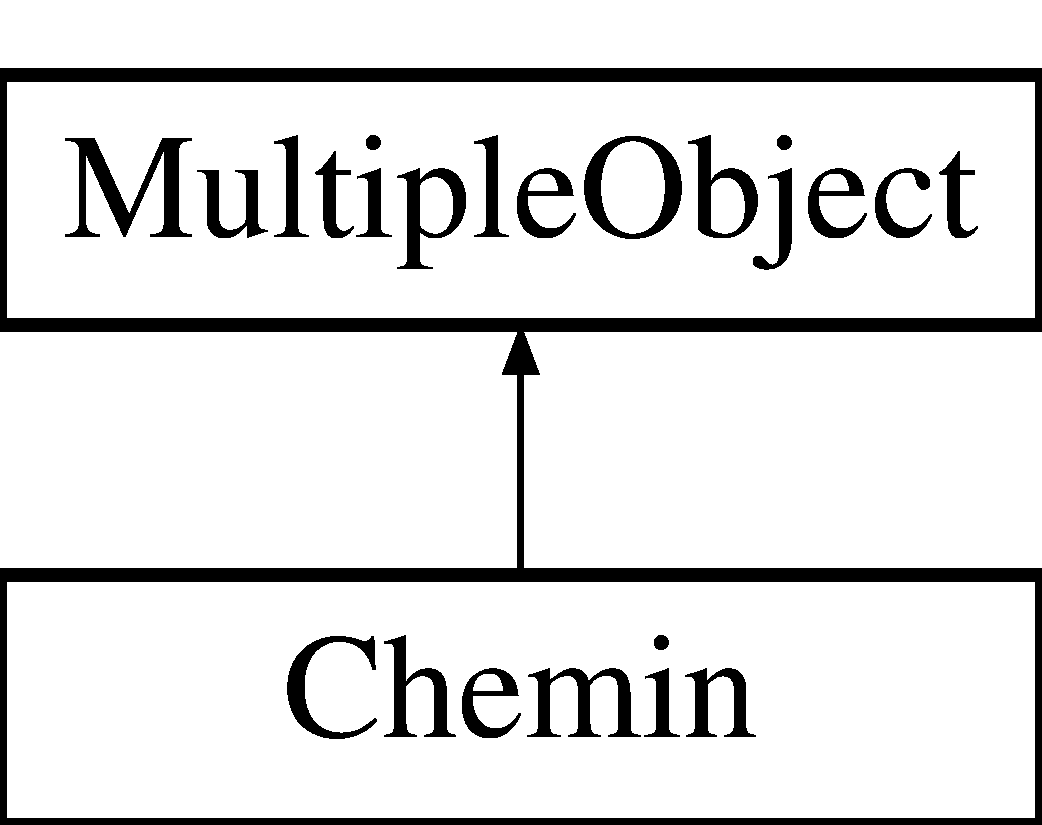
\includegraphics[height=2.000000cm]{classChemin}
\end{center}
\end{figure}
\subsection*{Fonctions membres publiques}
\begin{DoxyCompactItemize}
\item 
bool \hyperlink{classChemin_a2ee7b6a34082453fbdf890a49017aead}{add} (int8\-\_\-t x, int8\-\_\-t y) override
\item 
bool \hyperlink{classChemin_a1ee3f200283c2c401ef0ffd5800d946c}{remove} (int8\-\_\-t x, int8\-\_\-t y) override
\item 
bool \hyperlink{classChemin_aceccf541a2cdde27eb8f4bf541aff1b3}{has} (int8\-\_\-t x, int8\-\_\-t y) override
\item 
bool \hyperlink{classChemin_a67a8418164f0b2a4d1827e393ba859f7}{clear} () override
\item 
string \hyperlink{classChemin_a3b1754233eb79fb9f7d119a42efbda3c}{to\-String} () override
\item 
\hyperlink{classChemin_a0024ec1de3487b44a51c095aca1b83dc}{$\sim$\-Chemin} ()
\end{DoxyCompactItemize}
\subsection*{Fonctions membres publiques statiques}
\begin{DoxyCompactItemize}
\item 
static \hyperlink{classChemin}{Chemin} $\ast$ \hyperlink{classChemin_a82bfca776ad8bd221a5a430526f1d41f}{get\-Instance} ()
\end{DoxyCompactItemize}
\subsection*{Attributs publics}
\begin{DoxyCompactItemize}
\item 
vector$<$ pair$<$ int8\-\_\-t, int8\-\_\-t $>$ $>$ $\ast$ \hyperlink{classChemin_a5acfc655d74effb1ed6eb14494c017b0}{list\-\_\-chemin}
\end{DoxyCompactItemize}
\subsection*{Fonctions membres privées}
\begin{DoxyCompactItemize}
\item 
\hyperlink{classChemin_a5858339cc57c83e756c8412764990f16}{Chemin} ()
\end{DoxyCompactItemize}
\subsection*{Attributs privés statiques}
\begin{DoxyCompactItemize}
\item 
static \hyperlink{classChemin}{Chemin} $\ast$ \hyperlink{classChemin_a068df8f068a5609d0e2db8442f5e3a38}{instance} = nullptr
\end{DoxyCompactItemize}


\subsection{Documentation des constructeurs et destructeur}
\hypertarget{classChemin_a0024ec1de3487b44a51c095aca1b83dc}{\index{Chemin@{Chemin}!$\sim$\-Chemin@{$\sim$\-Chemin}}
\index{$\sim$\-Chemin@{$\sim$\-Chemin}!Chemin@{Chemin}}
\subsubsection[{$\sim$\-Chemin}]{\setlength{\rightskip}{0pt plus 5cm}Chemin\-::$\sim$\-Chemin (
\begin{DoxyParamCaption}
{}
\end{DoxyParamCaption}
)\hspace{0.3cm}{\ttfamily [inline]}}}\label{classChemin_a0024ec1de3487b44a51c095aca1b83dc}

\begin{DoxyCode}
30              \{
31         \textcolor{keyword}{delete} []\hyperlink{classChemin_a5acfc655d74effb1ed6eb14494c017b0}{list\_chemin};
32         \hyperlink{classChemin_a5acfc655d74effb1ed6eb14494c017b0}{list\_chemin} = \textcolor{keyword}{nullptr};
33         \textcolor{keyword}{delete} \hyperlink{classChemin_a068df8f068a5609d0e2db8442f5e3a38}{instance};
34         \hyperlink{classChemin_a068df8f068a5609d0e2db8442f5e3a38}{instance} = \textcolor{keyword}{nullptr};
35     \}
\end{DoxyCode}
\hypertarget{classChemin_a5858339cc57c83e756c8412764990f16}{\index{Chemin@{Chemin}!Chemin@{Chemin}}
\index{Chemin@{Chemin}!Chemin@{Chemin}}
\subsubsection[{Chemin}]{\setlength{\rightskip}{0pt plus 5cm}Chemin\-::\-Chemin (
\begin{DoxyParamCaption}
{}
\end{DoxyParamCaption}
)\hspace{0.3cm}{\ttfamily [inline]}, {\ttfamily [private]}}}\label{classChemin_a5858339cc57c83e756c8412764990f16}


Référencé par get\-Instance().


\begin{DoxyCode}
39             \{
40         \hyperlink{classChemin_a5acfc655d74effb1ed6eb14494c017b0}{list\_chemin} = \textcolor{keyword}{new} vector<pair<int8\_t, int8\_t>>();
41     \}
\end{DoxyCode}


\subsection{Documentation des fonctions membres}
\hypertarget{classChemin_a2ee7b6a34082453fbdf890a49017aead}{\index{Chemin@{Chemin}!add@{add}}
\index{add@{add}!Chemin@{Chemin}}
\subsubsection[{add}]{\setlength{\rightskip}{0pt plus 5cm}bool Chemin\-::add (
\begin{DoxyParamCaption}
\item[{int8\-\_\-t}]{x, }
\item[{int8\-\_\-t}]{y}
\end{DoxyParamCaption}
)\hspace{0.3cm}{\ttfamily [override]}, {\ttfamily [virtual]}}}\label{classChemin_a2ee7b6a34082453fbdf890a49017aead}


Implémente \hyperlink{classMultipleObject_aa5e743143bdedeb901c8e234162b3db1}{Multiple\-Object}.



Références list\-\_\-chemin.



Référencé par Core\-::pathfinding(), et unitest\-\_\-pathfinding().


\begin{DoxyCode}
16                                   \{
17     \hyperlink{classChemin_a5acfc655d74effb1ed6eb14494c017b0}{list\_chemin}->push\_back(std::make\_pair(x,y));
18     \textcolor{keywordflow}{return} std::find(\hyperlink{classChemin_a5acfc655d74effb1ed6eb14494c017b0}{list\_chemin}->begin(), \hyperlink{classChemin_a5acfc655d74effb1ed6eb14494c017b0}{list\_chemin}->end(), std::make\_pair(x,y)) 
      != \hyperlink{classChemin_a5acfc655d74effb1ed6eb14494c017b0}{list\_chemin}->end();
19 \}
\end{DoxyCode}
\hypertarget{classChemin_a67a8418164f0b2a4d1827e393ba859f7}{\index{Chemin@{Chemin}!clear@{clear}}
\index{clear@{clear}!Chemin@{Chemin}}
\subsubsection[{clear}]{\setlength{\rightskip}{0pt plus 5cm}bool Chemin\-::clear (
\begin{DoxyParamCaption}
{}
\end{DoxyParamCaption}
)\hspace{0.3cm}{\ttfamily [inline]}, {\ttfamily [override]}, {\ttfamily [virtual]}}}\label{classChemin_a67a8418164f0b2a4d1827e393ba859f7}


Implémente \hyperlink{classMultipleObject_a980acdfb99e25ec0d5e61396f60517c3}{Multiple\-Object}.



Référencé par Manager\-::reset().


\begin{DoxyCode}
25                          \{
26         \hyperlink{classChemin_a5acfc655d74effb1ed6eb14494c017b0}{list\_chemin}->clear();
27         \textcolor{keywordflow}{return} \hyperlink{classChemin_a5acfc655d74effb1ed6eb14494c017b0}{list\_chemin}->size() == 0;
28     \}
\end{DoxyCode}
\hypertarget{classChemin_a82bfca776ad8bd221a5a430526f1d41f}{\index{Chemin@{Chemin}!get\-Instance@{get\-Instance}}
\index{get\-Instance@{get\-Instance}!Chemin@{Chemin}}
\subsubsection[{get\-Instance}]{\setlength{\rightskip}{0pt plus 5cm}{\bf Chemin} $\ast$ Chemin\-::get\-Instance (
\begin{DoxyParamCaption}
{}
\end{DoxyParamCaption}
)\hspace{0.3cm}{\ttfamily [static]}}}\label{classChemin_a82bfca776ad8bd221a5a430526f1d41f}


Références Chemin(), et instance.



Référencé par Manager\-::\-Manager().


\begin{DoxyCode}
9                             \{
10     \textcolor{keywordflow}{if}(\hyperlink{classChemin_a068df8f068a5609d0e2db8442f5e3a38}{instance} == \textcolor{keyword}{nullptr})\{
11         \hyperlink{classChemin_a068df8f068a5609d0e2db8442f5e3a38}{instance} = \textcolor{keyword}{new} \hyperlink{classChemin_a5858339cc57c83e756c8412764990f16}{Chemin}();
12     \}
13     \textcolor{keywordflow}{return} \hyperlink{classChemin_a068df8f068a5609d0e2db8442f5e3a38}{instance};
14 \}
\end{DoxyCode}
\hypertarget{classChemin_aceccf541a2cdde27eb8f4bf541aff1b3}{\index{Chemin@{Chemin}!has@{has}}
\index{has@{has}!Chemin@{Chemin}}
\subsubsection[{has}]{\setlength{\rightskip}{0pt plus 5cm}bool Chemin\-::has (
\begin{DoxyParamCaption}
\item[{int8\-\_\-t}]{x, }
\item[{int8\-\_\-t}]{y}
\end{DoxyParamCaption}
)\hspace{0.3cm}{\ttfamily [override]}, {\ttfamily [virtual]}}}\label{classChemin_aceccf541a2cdde27eb8f4bf541aff1b3}


Implémente \hyperlink{classMultipleObject_a1703b0c461708fbb6985e87624f4b17b}{Multiple\-Object}.



Références list\-\_\-chemin.



Référencé par remove().


\begin{DoxyCode}
29                                   \{
30     \textcolor{keywordflow}{return} std::find(\hyperlink{classChemin_a5acfc655d74effb1ed6eb14494c017b0}{list\_chemin}->begin(), \hyperlink{classChemin_a5acfc655d74effb1ed6eb14494c017b0}{list\_chemin}->end(), std::make\_pair(x,y)) 
      != \hyperlink{classChemin_a5acfc655d74effb1ed6eb14494c017b0}{list\_chemin}->end();
31 \}
\end{DoxyCode}
\hypertarget{classChemin_a1ee3f200283c2c401ef0ffd5800d946c}{\index{Chemin@{Chemin}!remove@{remove}}
\index{remove@{remove}!Chemin@{Chemin}}
\subsubsection[{remove}]{\setlength{\rightskip}{0pt plus 5cm}bool Chemin\-::remove (
\begin{DoxyParamCaption}
\item[{int8\-\_\-t}]{x, }
\item[{int8\-\_\-t}]{y}
\end{DoxyParamCaption}
)\hspace{0.3cm}{\ttfamily [override]}, {\ttfamily [virtual]}}}\label{classChemin_a1ee3f200283c2c401ef0ffd5800d946c}


Implémente \hyperlink{classMultipleObject_ad57dd5fec65953bbce399afdca475a4c}{Multiple\-Object}.



Références has(), et list\-\_\-chemin.


\begin{DoxyCode}
21                                      \{
22     \textcolor{keywordflow}{if}(\hyperlink{classChemin_aceccf541a2cdde27eb8f4bf541aff1b3}{has}(x,y))\{
23         \hyperlink{classChemin_a5acfc655d74effb1ed6eb14494c017b0}{list\_chemin}->erase(std::remove(\hyperlink{classChemin_a5acfc655d74effb1ed6eb14494c017b0}{list\_chemin}->begin(), 
      \hyperlink{classChemin_a5acfc655d74effb1ed6eb14494c017b0}{list\_chemin}->end(), std::make\_pair(x,y)), \hyperlink{classChemin_a5acfc655d74effb1ed6eb14494c017b0}{list\_chemin}->end());
24         \textcolor{keywordflow}{return} !\hyperlink{classChemin_aceccf541a2cdde27eb8f4bf541aff1b3}{has}(x,y);
25     \}
26         \textcolor{keywordflow}{return} \textcolor{keyword}{true}; \textcolor{comment}{//default true if isn't in table.}
27 \}
\end{DoxyCode}
\hypertarget{classChemin_a3b1754233eb79fb9f7d119a42efbda3c}{\index{Chemin@{Chemin}!to\-String@{to\-String}}
\index{to\-String@{to\-String}!Chemin@{Chemin}}
\subsubsection[{to\-String}]{\setlength{\rightskip}{0pt plus 5cm}string Chemin\-::to\-String (
\begin{DoxyParamCaption}
{}
\end{DoxyParamCaption}
)\hspace{0.3cm}{\ttfamily [override]}, {\ttfamily [virtual]}}}\label{classChemin_a3b1754233eb79fb9f7d119a42efbda3c}


Implémente \hyperlink{classMultipleObject_a5439a2ac4cc86c759ef1df8f6059947a}{Multiple\-Object}.



Références list\-\_\-chemin.



Référencé par Manager\-::to\-String().


\begin{DoxyCode}
33                        \{
34     int16\_t size = \hyperlink{classChemin_a5acfc655d74effb1ed6eb14494c017b0}{list\_chemin}->size();
35     stringstream value;
36     value << \textcolor{stringliteral}{""};
37     int16\_t i =0;
38     std::for\_each(\hyperlink{classChemin_a5acfc655d74effb1ed6eb14494c017b0}{list\_chemin}->begin(), \hyperlink{classChemin_a5acfc655d74effb1ed6eb14494c017b0}{list\_chemin}->end(), [&](std::pair<int8\_t,
       int8\_t> \_b)\{
39         value << \textcolor{stringliteral}{"\(\backslash\)""}<<i<<\textcolor{stringliteral}{"\(\backslash\)": \(\backslash\)""}<<(int)\_b.first<< \textcolor{stringliteral}{","} <<(\textcolor{keywordtype}{int})\_b.second<<\textcolor{stringliteral}{"\(\backslash\)", "};
40         ++i;
41     \});
42     stringstream buf;
43     buf <<\textcolor{stringliteral}{" \(\backslash\)"Chemin\(\backslash\)": \{ \(\backslash\)"Number\(\backslash\)": "}<<size<<\textcolor{stringliteral}{", \(\backslash\)"Position\(\backslash\)": \{"}<<value.str().substr(0, value.str().size(
      )-2)<<\textcolor{stringliteral}{"\} \}"};
44     \textcolor{keywordflow}{return} buf.str();
45 \}\end{DoxyCode}


\subsection{Documentation des données membres}
\hypertarget{classChemin_a068df8f068a5609d0e2db8442f5e3a38}{\index{Chemin@{Chemin}!instance@{instance}}
\index{instance@{instance}!Chemin@{Chemin}}
\subsubsection[{instance}]{\setlength{\rightskip}{0pt plus 5cm}{\bf Chemin} $\ast$ Chemin\-::instance = nullptr\hspace{0.3cm}{\ttfamily [static]}, {\ttfamily [private]}}}\label{classChemin_a068df8f068a5609d0e2db8442f5e3a38}


Référencé par get\-Instance().

\hypertarget{classChemin_a5acfc655d74effb1ed6eb14494c017b0}{\index{Chemin@{Chemin}!list\-\_\-chemin@{list\-\_\-chemin}}
\index{list\-\_\-chemin@{list\-\_\-chemin}!Chemin@{Chemin}}
\subsubsection[{list\-\_\-chemin}]{\setlength{\rightskip}{0pt plus 5cm}vector$<$pair$<$int8\-\_\-t,int8\-\_\-t$>$ $>$$\ast$ Chemin\-::list\-\_\-chemin}}\label{classChemin_a5acfc655d74effb1ed6eb14494c017b0}


Référencé par add(), Core\-::draw\-Debug(), has(), remove(), to\-String(), et Manager\-::update().



La documentation de cette classe a été générée à partir des fichiers suivants \-:\begin{DoxyCompactItemize}
\item 
headers/manager/\hyperlink{chemin_8h}{chemin.\-h}\item 
sources/\hyperlink{chemin_8cpp}{chemin.\-cpp}\end{DoxyCompactItemize}

\hypertarget{classClient}{\section{Référence de la classe Client}
\label{classClient}\index{Client@{Client}}
}


{\ttfamily \#include $<$client.\-h$>$}

\subsection*{Fonctions membres publiques}
\begin{DoxyCompactItemize}
\item 
\hyperlink{classClient_ae51af7aa6b8f591496a8f6a4a87a14bf}{Client} ()
\end{DoxyCompactItemize}
\subsection*{Attributs publics}
\begin{DoxyCompactItemize}
\item 
std\-::string \hyperlink{classClient_af29655fb85148cf9cff9c94af770c023}{m\-\_\-id}
\item 
uint16\-\_\-t \hyperlink{classClient_a80564d281c880f1e80b6e1b54ae6e71e}{m\-\_\-sock}
\end{DoxyCompactItemize}


\subsection{Documentation des constructeurs et destructeur}
\hypertarget{classClient_ae51af7aa6b8f591496a8f6a4a87a14bf}{\index{Client@{Client}!Client@{Client}}
\index{Client@{Client}!Client@{Client}}
\subsubsection[{Client}]{\setlength{\rightskip}{0pt plus 5cm}Client\-::\-Client (
\begin{DoxyParamCaption}
{}
\end{DoxyParamCaption}
)\hspace{0.3cm}{\ttfamily [inline]}}}\label{classClient_ae51af7aa6b8f591496a8f6a4a87a14bf}


Références m\-\_\-id.


\begin{DoxyCode}
17             \{
18       \hyperlink{classClient_af29655fb85148cf9cff9c94af770c023}{m\_id} = \textcolor{stringliteral}{""};
19     \}
\end{DoxyCode}


\subsection{Documentation des données membres}
\hypertarget{classClient_af29655fb85148cf9cff9c94af770c023}{\index{Client@{Client}!m\-\_\-id@{m\-\_\-id}}
\index{m\-\_\-id@{m\-\_\-id}!Client@{Client}}
\subsubsection[{m\-\_\-id}]{\setlength{\rightskip}{0pt plus 5cm}std\-::string Client\-::m\-\_\-id}}\label{classClient_af29655fb85148cf9cff9c94af770c023}


Référencé par Serveur\-::\-Accept\-And\-Dispatch(), Client(), et Serveur\-::synchronize\-Client().

\hypertarget{classClient_a80564d281c880f1e80b6e1b54ae6e71e}{\index{Client@{Client}!m\-\_\-sock@{m\-\_\-sock}}
\index{m\-\_\-sock@{m\-\_\-sock}!Client@{Client}}
\subsubsection[{m\-\_\-sock}]{\setlength{\rightskip}{0pt plus 5cm}uint16\-\_\-t Client\-::m\-\_\-sock}}\label{classClient_a80564d281c880f1e80b6e1b54ae6e71e}


Référencé par Serveur\-::\-Accept\-And\-Dispatch(), Serveur\-::receive(), et Serveur\-::send\-To\-Client().



La documentation de cette classe a été générée à partir du fichier suivant \-:\begin{DoxyCompactItemize}
\item 
headers/serveur/\hyperlink{client_8h}{client.\-h}\end{DoxyCompactItemize}

\hypertarget{classCore}{\section{Référence de la classe Core}
\label{classCore}\index{Core@{Core}}
}


{\ttfamily \#include $<$core.\-h$>$}

\subsection*{Fonctions membres publiques}
\begin{DoxyCompactItemize}
\item 
\hyperlink{classCore_a14e63188e0aa7c4a6f72d5501384d1f9}{Core} ()
\item 
\hyperlink{classCore_a776f8c46504b14183883c6273f93eaed}{$\sim$\-Core} ()
\item 
bool \hyperlink{classCore_a722434c9873d07d6b26a74e40e08eb9c}{start} ()
\item 
bool \hyperlink{classCore_a01ec355d4fc9be14623bb7b249ad9562}{stop} ()
\item 
bool \hyperlink{classCore_a85d7a4a5672973830aa10185b121ded9}{reset} ()
\end{DoxyCompactItemize}
\subsection*{Fonctions membres privées}
\begin{DoxyCompactItemize}
\item 
void \hyperlink{classCore_ae03caf8d8abe9d4c3b875c6f6a5d40dd}{draw\-Debug} (Mat \&frame)
\item 
bool \hyperlink{classCore_a2ad48b714f575d3f3c25c80ffa72afad}{init} ()
\item 
bool \hyperlink{classCore_a2197457d525b6f0eface1f8712fd2084}{restart\-Server} ()
\item 
void \hyperlink{classCore_a1dac5f63296f11309c2f25770b30912b}{set\-Mode} (\hyperlink{core_8h_a46c8a310cf4c094f8c80e1cb8dc1f911}{Mode} \-\_\-mode)
\item 
\hyperlink{core_8h_a46c8a310cf4c094f8c80e1cb8dc1f911}{Mode} \hyperlink{classCore_a0d0ccf9b40761ed8f88fe1d9a348fc02}{get\-Current\-Mode} ()
\item 
void \hyperlink{classCore_a9677503611528b6d6f2039eff6f80912}{listen\-I\-P\-C} ()
\item 
void \hyperlink{classCore_a7fab8414125602f9f595143bb21d24c1}{auto\-Virtual\-Mode} (bool is\-\_\-auto)
\item 
void \hyperlink{classCore_afcdd1611a6528fd3d597d719405493b4}{manual\-Mode} ()
\item 
\hyperlink{core_8h_a5d74787dedbc4e11c1ab15bf487e61f8}{State} \hyperlink{classCore_a2d832a5e544b5e76d03a7fd596522b42}{calibration} ()
\item 
\hyperlink{core_8h_a5d74787dedbc4e11c1ab15bf487e61f8}{State} \hyperlink{classCore_a8648fac82f0324cead88c8fa2731b286}{block\-Processing} (bool is\-\_\-auto)
\item 
\hyperlink{core_8h_a5d74787dedbc4e11c1ab15bf487e61f8}{State} \hyperlink{classCore_a333060e38c961d6fbf4ba4d01a84e48b}{pathfinding} ()
\item 
\hyperlink{core_8h_a5d74787dedbc4e11c1ab15bf487e61f8}{State} \hyperlink{classCore_a2a8efb95fadd86481ba62c98b72c7f1c}{server} ()
\item 
\hyperlink{core_8h_a5d74787dedbc4e11c1ab15bf487e61f8}{State} \hyperlink{classCore_a185801ec33fe24b0f36e4d9e474403ca}{trajectory} ()
\item 
bool \hyperlink{classCore_a180fe625431721a94959a694fe91ef3f}{forward} (float angle)
\item 
bool \hyperlink{classCore_a0639e803afd1447272759b6b0fa22f60}{rotation} (float angle)
\end{DoxyCompactItemize}
\subsection*{Attributs privés}
\begin{DoxyCompactItemize}
\item 
struct \hyperlink{core_8h_struct__stateMachine}{\-\_\-state\-Machine} \hyperlink{classCore_a2eaa56d6855905faec8a1764db40892b}{state\-Machine}
\item 
bool \hyperlink{classCore_a92f7a9f089b3dca665ec0537fb554d1b}{change\-Mode}
\item 
\hyperlink{core_8h_a46c8a310cf4c094f8c80e1cb8dc1f911}{Mode} \hyperlink{classCore_a05fa4660e945441b917880d1e148c89a}{avm\-\_\-mode}
\item 
\hyperlink{classManager}{Manager} $\ast$ \hyperlink{classCore_a834f8de7a2b8f18b19af83d6c05b9b3a}{manager}
\item 
\hyperlink{classImagesP}{Images\-P} $\ast$ \hyperlink{classCore_a7a18e37fde7d3ca4b1568225b51eaf0d}{process}
\item 
\hyperlink{classPathFinding}{Path\-Finding} $\ast$ \hyperlink{classCore_a55b925c8acc13a0002112d48a054984e}{path}
\end{DoxyCompactItemize}


\subsection{Documentation des constructeurs et destructeur}
\hypertarget{classCore_a14e63188e0aa7c4a6f72d5501384d1f9}{\index{Core@{Core}!Core@{Core}}
\index{Core@{Core}!Core@{Core}}
\subsubsection[{Core}]{\setlength{\rightskip}{0pt plus 5cm}Core\-::\-Core (
\begin{DoxyParamCaption}
{}
\end{DoxyParamCaption}
)}}\label{classCore_a14e63188e0aa7c4a6f72d5501384d1f9}


Références init().


\begin{DoxyCode}
5           \{
6     \hyperlink{classCore_a2ad48b714f575d3f3c25c80ffa72afad}{init}();
7 \}
\end{DoxyCode}
\hypertarget{classCore_a776f8c46504b14183883c6273f93eaed}{\index{Core@{Core}!$\sim$\-Core@{$\sim$\-Core}}
\index{$\sim$\-Core@{$\sim$\-Core}!Core@{Core}}
\subsubsection[{$\sim$\-Core}]{\setlength{\rightskip}{0pt plus 5cm}Core\-::$\sim$\-Core (
\begin{DoxyParamCaption}
{}
\end{DoxyParamCaption}
)}}\label{classCore_a776f8c46504b14183883c6273f93eaed}


Références manager, path, et process.


\begin{DoxyCode}
9            \{
10     \textcolor{keyword}{delete} \hyperlink{classCore_a55b925c8acc13a0002112d48a054984e}{path};
11     \hyperlink{classCore_a55b925c8acc13a0002112d48a054984e}{path} = \textcolor{keyword}{nullptr};
12     \textcolor{keyword}{delete} \hyperlink{classCore_a7a18e37fde7d3ca4b1568225b51eaf0d}{process};
13     \hyperlink{classCore_a7a18e37fde7d3ca4b1568225b51eaf0d}{process} = \textcolor{keyword}{nullptr};
14     \textcolor{keyword}{delete} \hyperlink{classCore_a834f8de7a2b8f18b19af83d6c05b9b3a}{manager};
15     \hyperlink{classCore_a834f8de7a2b8f18b19af83d6c05b9b3a}{manager} = \textcolor{keyword}{nullptr};
16 \}
\end{DoxyCode}


\subsection{Documentation des fonctions membres}
\hypertarget{classCore_a7fab8414125602f9f595143bb21d24c1}{\index{Core@{Core}!auto\-Virtual\-Mode@{auto\-Virtual\-Mode}}
\index{auto\-Virtual\-Mode@{auto\-Virtual\-Mode}!Core@{Core}}
\subsubsection[{auto\-Virtual\-Mode}]{\setlength{\rightskip}{0pt plus 5cm}void Core\-::auto\-Virtual\-Mode (
\begin{DoxyParamCaption}
\item[{bool}]{is\-\_\-auto}
\end{DoxyParamCaption}
)\hspace{0.3cm}{\ttfamily [private]}}}\label{classCore_a7fab8414125602f9f595143bb21d24c1}


Références \-\_\-state\-Machine\-::\-\_\-state\-Calibration, \-\_\-state\-Machine\-::\-\_\-state\-Image\-Block, \-\_\-state\-Machine\-::\-\_\-state\-Pathfinding, \-\_\-state\-Machine\-::\-\_\-state\-Server, \-\_\-state\-Machine\-::\-\_\-state\-Trajectory, block\-Processing(), calibration(), D\-E\-B\-U\-G, E\-R\-R\-O\-R, N\-O, N\-O\-N\-E, O\-K, pathfinding(), server(), set\-Mode(), state\-Machine, Stop\-\_\-\-Mode, et trajectory().



Référencé par start().


\begin{DoxyCode}
117                                       \{
118     \textcolor{keywordflow}{if}(\hyperlink{classCore_a2eaa56d6855905faec8a1764db40892b}{stateMachine}.\hyperlink{core_8h_aaee24e4ab99a6f1243a46645188de8d0}{\_stateServer} == \hyperlink{core_8h_a5d74787dedbc4e11c1ab15bf487e61f8ab50339a10e1de285ac99d4c3990b8693}{State::NONE} || 
      \hyperlink{classCore_a2eaa56d6855905faec8a1764db40892b}{stateMachine}.\hyperlink{core_8h_aaee24e4ab99a6f1243a46645188de8d0}{\_stateServer} == \hyperlink{core_8h_a5d74787dedbc4e11c1ab15bf487e61f8ac2f3f489a00553e7a01d369c103c7251}{State::NO})\{
119         \hyperlink{classCore_a2eaa56d6855905faec8a1764db40892b}{stateMachine}.\hyperlink{core_8h_aaee24e4ab99a6f1243a46645188de8d0}{\_stateServer} = \hyperlink{classCore_a2a8efb95fadd86481ba62c98b72c7f1c}{server}();
120     \}\textcolor{keywordflow}{else} \textcolor{keywordflow}{if}(\hyperlink{classCore_a2eaa56d6855905faec8a1764db40892b}{stateMachine}.\hyperlink{core_8h_aaee24e4ab99a6f1243a46645188de8d0}{\_stateServer} == \hyperlink{core_8h_a5d74787dedbc4e11c1ab15bf487e61f8abb1ca97ec761fc37101737ba0aa2e7c5}{State::ERROR})\{
121         \textcolor{comment}{//TODO ERROR ecrit dans un fichier de log une erreur}
122     \}
123 \textcolor{keywordflow}{else} \textcolor{keywordflow}{if}(\hyperlink{classCore_a2eaa56d6855905faec8a1764db40892b}{stateMachine}.\hyperlink{core_8h_aaee24e4ab99a6f1243a46645188de8d0}{\_stateServer} == \hyperlink{core_8h_a5d74787dedbc4e11c1ab15bf487e61f8ae0aa021e21dddbd6d8cecec71e9cf564}{State::OK})\{
124         \textcolor{keywordflow}{if}(\hyperlink{definition_8h_a117352cc494cc62c6b2f1882786a332c}{DEBUG}) std::cout<<\textcolor{stringliteral}{"SERVER OK"}<<std::endl;
125         \textcolor{keywordflow}{if}(\hyperlink{classCore_a2eaa56d6855905faec8a1764db40892b}{stateMachine}.\hyperlink{core_8h_a157036ced733a021849ebcbc98c27200}{\_stateCalibration} == 
      \hyperlink{core_8h_a5d74787dedbc4e11c1ab15bf487e61f8ab50339a10e1de285ac99d4c3990b8693}{State::NONE})\{
126             \hyperlink{classCore_a2d832a5e544b5e76d03a7fd596522b42}{calibration}();
127         \}\textcolor{keywordflow}{else} \textcolor{keywordflow}{if}(\hyperlink{classCore_a2eaa56d6855905faec8a1764db40892b}{stateMachine}.\hyperlink{core_8h_a157036ced733a021849ebcbc98c27200}{\_stateCalibration} == 
      \hyperlink{core_8h_a5d74787dedbc4e11c1ab15bf487e61f8abb1ca97ec761fc37101737ba0aa2e7c5}{State::ERROR})\{
128             \textcolor{comment}{//TODO NO CENTER OF AREA NO FOUND, turn arround car}
129             \textcolor{keywordflow}{if}(\hyperlink{definition_8h_a117352cc494cc62c6b2f1882786a332c}{DEBUG}) std::cout<<\textcolor{stringliteral}{"CALIBRATION FAILED (no QRcenter)"}<<std::endl;
130         \}
131     \textcolor{keywordflow}{else} \textcolor{keywordflow}{if}(\hyperlink{classCore_a2eaa56d6855905faec8a1764db40892b}{stateMachine}.\hyperlink{core_8h_a157036ced733a021849ebcbc98c27200}{\_stateCalibration} == 
      \hyperlink{core_8h_a5d74787dedbc4e11c1ab15bf487e61f8ae0aa021e21dddbd6d8cecec71e9cf564}{State::OK})\{
132             \textcolor{keywordflow}{if}(\hyperlink{definition_8h_a117352cc494cc62c6b2f1882786a332c}{DEBUG}) std::cout<<\textcolor{stringliteral}{"CALIBRATION OK"}<<std::endl;
133             \textcolor{keywordflow}{if}(\hyperlink{classCore_a2eaa56d6855905faec8a1764db40892b}{stateMachine}.\hyperlink{core_8h_adbc0e51d4bed9b6da5c44e921e37dc32}{\_stateImageBlock} == 
      \hyperlink{core_8h_a5d74787dedbc4e11c1ab15bf487e61f8ab50339a10e1de285ac99d4c3990b8693}{State::NONE})\{
134                 \hyperlink{classCore_a8648fac82f0324cead88c8fa2731b286}{blockProcessing}(is\_auto);
135             \}\textcolor{keywordflow}{else} \textcolor{keywordflow}{if}(\hyperlink{classCore_a2eaa56d6855905faec8a1764db40892b}{stateMachine}.\hyperlink{core_8h_adbc0e51d4bed9b6da5c44e921e37dc32}{\_stateImageBlock} == 
      \hyperlink{core_8h_a5d74787dedbc4e11c1ab15bf487e61f8abb1ca97ec761fc37101737ba0aa2e7c5}{State::ERROR})\{
136                 \textcolor{comment}{//TODO ERROR detect block > 3 (Arrival, Car and Area) and 0 case found (Block devide 9)}
137                 \textcolor{keywordflow}{if}(\hyperlink{definition_8h_a117352cc494cc62c6b2f1882786a332c}{DEBUG}) std::cout<<\textcolor{stringliteral}{"IMAGES PROCESSING FAILED (no case found 1 of 9x9)"}<<std::endl;
138             \}
139         \textcolor{keywordflow}{else} \textcolor{keywordflow}{if}(\hyperlink{classCore_a2eaa56d6855905faec8a1764db40892b}{stateMachine}.\hyperlink{core_8h_adbc0e51d4bed9b6da5c44e921e37dc32}{\_stateImageBlock} == 
      \hyperlink{core_8h_a5d74787dedbc4e11c1ab15bf487e61f8ae0aa021e21dddbd6d8cecec71e9cf564}{State::OK})\{
140                 \textcolor{keywordflow}{if}(\hyperlink{definition_8h_a117352cc494cc62c6b2f1882786a332c}{DEBUG}) std::cout<<\textcolor{stringliteral}{"IMAGES BLOCK OK"}<<std::endl;
141                 \textcolor{keywordflow}{if}(\hyperlink{classCore_a2eaa56d6855905faec8a1764db40892b}{stateMachine}.\hyperlink{core_8h_a79ce614ae01c3759d155c03026384ca7}{\_statePathfinding} == 
      \hyperlink{core_8h_a5d74787dedbc4e11c1ab15bf487e61f8ab50339a10e1de285ac99d4c3990b8693}{State::NONE})\{
142                     \hyperlink{classCore_a333060e38c961d6fbf4ba4d01a84e48b}{pathfinding}();
143                 \}\textcolor{keywordflow}{else} \textcolor{keywordflow}{if}(\hyperlink{classCore_a2eaa56d6855905faec8a1764db40892b}{stateMachine}.\hyperlink{core_8h_a79ce614ae01c3759d155c03026384ca7}{\_statePathfinding} == 
      \hyperlink{core_8h_a5d74787dedbc4e11c1ab15bf487e61f8ac2f3f489a00553e7a01d369c103c7251}{State::NO})\{
144                     \textcolor{comment}{//TODO no possibility to found arrival}
145                     \textcolor{keywordflow}{if}(\hyperlink{definition_8h_a117352cc494cc62c6b2f1882786a332c}{DEBUG}) std::cout<<\textcolor{stringliteral}{"NO POSSIBILITY PATHFINDING"}<<std::endl;
146                 \}
147             \textcolor{keywordflow}{else} \textcolor{keywordflow}{if}(\hyperlink{classCore_a2eaa56d6855905faec8a1764db40892b}{stateMachine}.\hyperlink{core_8h_a79ce614ae01c3759d155c03026384ca7}{\_statePathfinding} == 
      \hyperlink{core_8h_a5d74787dedbc4e11c1ab15bf487e61f8ae0aa021e21dddbd6d8cecec71e9cf564}{State::OK})\{
148                     \textcolor{keywordflow}{if}(\hyperlink{definition_8h_a117352cc494cc62c6b2f1882786a332c}{DEBUG}) std::cout<<\textcolor{stringliteral}{"PATHFINDING OK"}<<std::endl;
149                     \textcolor{keywordflow}{if}(\hyperlink{classCore_a2eaa56d6855905faec8a1764db40892b}{stateMachine}.\hyperlink{core_8h_a88c6e0c15cdd29b3eec2e842fa09b08f}{\_stateTrajectory} == 
      \hyperlink{core_8h_a5d74787dedbc4e11c1ab15bf487e61f8ab50339a10e1de285ac99d4c3990b8693}{State::NONE})\{
150                         \hyperlink{classCore_a185801ec33fe24b0f36e4d9e474403ca}{trajectory}();
151                     \}\textcolor{keywordflow}{else} \textcolor{keywordflow}{if}(\hyperlink{classCore_a2eaa56d6855905faec8a1764db40892b}{stateMachine}.\hyperlink{core_8h_a88c6e0c15cdd29b3eec2e842fa09b08f}{\_stateTrajectory} == 
      \hyperlink{core_8h_a5d74787dedbc4e11c1ab15bf487e61f8abb1ca97ec761fc37101737ba0aa2e7c5}{State::ERROR})\{
152                         \textcolor{comment}{//TODO Car is blocked or some things like this}
153                         \textcolor{keywordflow}{if}(\hyperlink{definition_8h_a117352cc494cc62c6b2f1882786a332c}{DEBUG}) std::cout<<\textcolor{stringliteral}{"CAR is blocked"}<<std::endl;
154                     \}
155                 \textcolor{keywordflow}{else} \textcolor{keywordflow}{if}(\hyperlink{classCore_a2eaa56d6855905faec8a1764db40892b}{stateMachine}.\hyperlink{core_8h_a88c6e0c15cdd29b3eec2e842fa09b08f}{\_stateTrajectory} == 
      \hyperlink{core_8h_a5d74787dedbc4e11c1ab15bf487e61f8ae0aa021e21dddbd6d8cecec71e9cf564}{State::OK})\{
156                         \textcolor{comment}{//TODO Car is on Arrival !!}
157                         \hyperlink{classCore_a1dac5f63296f11309c2f25770b30912b}{setMode}(\hyperlink{core_8h_a46c8a310cf4c094f8c80e1cb8dc1f911acf535b39ede8798cd6b56d99271afeef}{Mode::Stop\_Mode}); \textcolor{comment}{//wait new }
158                     \}
159                 \}
160             \}
161         \}
162     \}
163 \}
\end{DoxyCode}
\hypertarget{classCore_a8648fac82f0324cead88c8fa2731b286}{\index{Core@{Core}!block\-Processing@{block\-Processing}}
\index{block\-Processing@{block\-Processing}!Core@{Core}}
\subsubsection[{block\-Processing}]{\setlength{\rightskip}{0pt plus 5cm}{\bf State} Core\-::block\-Processing (
\begin{DoxyParamCaption}
\item[{bool}]{is\-\_\-auto}
\end{DoxyParamCaption}
)\hspace{0.3cm}{\ttfamily [private]}}}\label{classCore_a8648fac82f0324cead88c8fa2731b286}


Références \-\_\-state\-Machine\-::\-\_\-state\-Image\-Block, Bloc\-::add(), Images\-P\-::all\-\_\-block, Manager\-::arrive, Manager\-::bloc, Manager\-::car, D\-E\-B\-U\-G, E\-R\-R\-O\-R, Images\-P\-::get\-Arrival\-Position(), Images\-P\-::get\-Car\-Position(), Images\-P\-::get\-Size\-Marker(), manager, O\-K, process, Car\-::set\-Position(), Arrive\-::set\-Position(), Images\-P\-::start\-Block(), state\-Machine, et Manager\-::update().



Référencé par auto\-Virtual\-Mode().


\begin{DoxyCode}
193                                        \{
194     \textcolor{keywordflow}{if}(is\_auto)\{
195         \textcolor{keywordflow}{if}(\hyperlink{definition_8h_a117352cc494cc62c6b2f1882786a332c}{DEBUG}) std::cout<<\textcolor{stringliteral}{"SEARCH BLOCK ... "};
196         \hyperlink{classCore_a7a18e37fde7d3ca4b1568225b51eaf0d}{process}->\hyperlink{classImagesP_ae2aecf8db20e7b3bcd14a7182dfdaf29}{startBlock}();
197         \textcolor{keywordflow}{for}(int8\_t i=0; i<\hyperlink{classCore_a7a18e37fde7d3ca4b1568225b51eaf0d}{process}->\hyperlink{classImagesP_ab9e279526694a7ce421cfa11b9309ed1}{all\_block}.size();++i)\{
198             \hyperlink{classCore_a834f8de7a2b8f18b19af83d6c05b9b3a}{manager}->\hyperlink{classManager_a66599bf2bd10c95b9fb7be9c333e0ff9}{bloc}->\hyperlink{classBloc_a02db4c95699ce40e8ad671ef759ebdb7}{add}(\hyperlink{classCore_a7a18e37fde7d3ca4b1568225b51eaf0d}{process}->\hyperlink{classImagesP_ab9e279526694a7ce421cfa11b9309ed1}{all\_block}.at(i).x, 
      \hyperlink{classCore_a7a18e37fde7d3ca4b1568225b51eaf0d}{process}->\hyperlink{classImagesP_ab9e279526694a7ce421cfa11b9309ed1}{all\_block}.at(i).y);
199         \}
200         \textcolor{keywordflow}{if}(\hyperlink{definition_8h_a117352cc494cc62c6b2f1882786a332c}{DEBUG}) std::cout<<\hyperlink{classCore_a7a18e37fde7d3ca4b1568225b51eaf0d}{process}->\hyperlink{classImagesP_ab9e279526694a7ce421cfa11b9309ed1}{all\_block}.size()<<\textcolor{stringliteral}{" FOUNDING"}<<std::endl;
201         \hyperlink{classCore_a834f8de7a2b8f18b19af83d6c05b9b3a}{manager}->\hyperlink{classManager_a2803dff8e8f2912242f4098991d91415}{car}->\hyperlink{classCar_a97e3c5de8eb65659ef520de6591f814d}{setPosition}(\hyperlink{classCore_a7a18e37fde7d3ca4b1568225b51eaf0d}{process}->
      \hyperlink{classImagesP_afe9cff50f49fc67bd8938d8d0223fe81}{getCarPosition}().x, \hyperlink{classCore_a7a18e37fde7d3ca4b1568225b51eaf0d}{process}->\hyperlink{classImagesP_afe9cff50f49fc67bd8938d8d0223fe81}{getCarPosition}().y);
202         \hyperlink{classCore_a834f8de7a2b8f18b19af83d6c05b9b3a}{manager}->\hyperlink{classManager_a6f99d8e25fc61a7fe0fdf160610b31cf}{arrive}->\hyperlink{classArrive_ab0484a9338e3774c5fa824153b1470e2}{setPosition}(\hyperlink{classCore_a7a18e37fde7d3ca4b1568225b51eaf0d}{process}->
      \hyperlink{classImagesP_aaf0d33634f747f1defec833fbc6dfae2}{getArrivalPosition}().x, \hyperlink{classCore_a7a18e37fde7d3ca4b1568225b51eaf0d}{process}->\hyperlink{classImagesP_aaf0d33634f747f1defec833fbc6dfae2}{getArrivalPosition}().y);
203         \hyperlink{classCore_a834f8de7a2b8f18b19af83d6c05b9b3a}{manager}->\hyperlink{classManager_af43da42550bd9746c5ea61a6aeee80de}{update}();
204         \textcolor{keywordflow}{if}((\textcolor{keywordtype}{int})\hyperlink{classCore_a7a18e37fde7d3ca4b1568225b51eaf0d}{process}->\hyperlink{classImagesP_a002bb2f3148a85c46c954dcc98ad2760}{getSizeMarker}() >= 2)\{
205             \hyperlink{classCore_a2eaa56d6855905faec8a1764db40892b}{stateMachine}.\hyperlink{core_8h_adbc0e51d4bed9b6da5c44e921e37dc32}{\_stateImageBlock} = 
      \hyperlink{core_8h_a5d74787dedbc4e11c1ab15bf487e61f8ae0aa021e21dddbd6d8cecec71e9cf564}{State::OK};
206         \}
207         \textcolor{keywordflow}{else}\{
208             \hyperlink{classCore_a2eaa56d6855905faec8a1764db40892b}{stateMachine}.\hyperlink{core_8h_adbc0e51d4bed9b6da5c44e921e37dc32}{\_stateImageBlock} = 
      \hyperlink{core_8h_a5d74787dedbc4e11c1ab15bf487e61f8abb1ca97ec761fc37101737ba0aa2e7c5}{State::ERROR};
209         \}
210     \}
211     \textcolor{keywordflow}{return} \hyperlink{core_8h_a5d74787dedbc4e11c1ab15bf487e61f8ae0aa021e21dddbd6d8cecec71e9cf564}{State::OK};
212 \}
\end{DoxyCode}
\hypertarget{classCore_a2d832a5e544b5e76d03a7fd596522b42}{\index{Core@{Core}!calibration@{calibration}}
\index{calibration@{calibration}!Core@{Core}}
\subsubsection[{calibration}]{\setlength{\rightskip}{0pt plus 5cm}{\bf State} Core\-::calibration (
\begin{DoxyParamCaption}
{}
\end{DoxyParamCaption}
)\hspace{0.3cm}{\ttfamily [private]}}}\label{classCore_a2d832a5e544b5e76d03a7fd596522b42}


Références \-\_\-state\-Machine\-::\-\_\-state\-Calibration, Images\-P\-::calibration(), E\-R\-R\-O\-R, Images\-P\-::load\-Calib(), O\-K, process, et state\-Machine.



Référencé par auto\-Virtual\-Mode().


\begin{DoxyCode}
181                        \{
182     \textcolor{keywordflow}{if}(\hyperlink{classCore_a7a18e37fde7d3ca4b1568225b51eaf0d}{process} == \textcolor{keyword}{nullptr})
183         \hyperlink{classCore_a7a18e37fde7d3ca4b1568225b51eaf0d}{process} = \textcolor{keyword}{new} \hyperlink{classImagesP}{ImagesP}();
184     \hyperlink{classCore_a7a18e37fde7d3ca4b1568225b51eaf0d}{process}->\hyperlink{classImagesP_a799c4550d96659d7d188b03f52bb9f4a}{calibration}();
185     \textcolor{keywordflow}{if}(\hyperlink{classCore_a7a18e37fde7d3ca4b1568225b51eaf0d}{process}->\hyperlink{classImagesP_a4048e5f515cb51cbf25211ec8b4854b7}{loadCalib}() != Point2f(-1,-1))\{
186         \hyperlink{classCore_a2eaa56d6855905faec8a1764db40892b}{stateMachine}.\hyperlink{core_8h_a157036ced733a021849ebcbc98c27200}{\_stateCalibration} = \hyperlink{core_8h_a5d74787dedbc4e11c1ab15bf487e61f8ae0aa021e21dddbd6d8cecec71e9cf564}{State::OK};
187     \}\textcolor{keywordflow}{else}\{
188         \hyperlink{classCore_a2eaa56d6855905faec8a1764db40892b}{stateMachine}.\hyperlink{core_8h_a157036ced733a021849ebcbc98c27200}{\_stateCalibration} = 
      \hyperlink{core_8h_a5d74787dedbc4e11c1ab15bf487e61f8abb1ca97ec761fc37101737ba0aa2e7c5}{State::ERROR};
189     \}
190     \textcolor{keywordflow}{return} \hyperlink{core_8h_a5d74787dedbc4e11c1ab15bf487e61f8ae0aa021e21dddbd6d8cecec71e9cf564}{State::OK};
191 \}
\end{DoxyCode}
\hypertarget{classCore_ae03caf8d8abe9d4c3b875c6f6a5d40dd}{\index{Core@{Core}!draw\-Debug@{draw\-Debug}}
\index{draw\-Debug@{draw\-Debug}!Core@{Core}}
\subsubsection[{draw\-Debug}]{\setlength{\rightskip}{0pt plus 5cm}void Core\-::draw\-Debug (
\begin{DoxyParamCaption}
\item[{Mat \&}]{frame}
\end{DoxyParamCaption}
)\hspace{0.3cm}{\ttfamily [private]}}}\label{classCore_ae03caf8d8abe9d4c3b875c6f6a5d40dd}


Références Manager\-::arrive, Manager\-::bloc, Manager\-::car, Manager\-::chemin, Car\-::get\-Position(), Arrive\-::get\-Position(), Bloc\-::list\-\_\-bloc, Chemin\-::list\-\_\-chemin, et manager.



Référencé par start().


\begin{DoxyCode}
18                               \{
19     \textcolor{keywordtype}{int} RecX1 = 240-240;
20     \textcolor{keywordtype}{int} RecX2 = 240+240;
21     \textcolor{keywordtype}{int} RecY1 = 240-240;
22     \textcolor{keywordtype}{int} RecY2 = 240+240;
23     \textcolor{keywordflow}{for}(\textcolor{keywordtype}{int} j=1; j<25;j++)\{
24         RecX2 = RecX2 - 20;
25         rectangle(frame, Point(RecX1, RecY1), Point(RecX2, RecY2), cv::Scalar(0, 255, 0));
26     \}
27     RecX2 = 240+240;
28     \textcolor{comment}{//horizontal}
29     \textcolor{keywordflow}{for}(\textcolor{keywordtype}{int} j=1; j<25;j++)\{
30         RecY2 = RecY2 - 20;
31         rectangle(frame, Point(RecX1, RecY1), Point(RecX2, RecY2), cv::Scalar(0, 255, 0));
32     \}
33     \textcolor{keywordflow}{if}(\hyperlink{classCore_a834f8de7a2b8f18b19af83d6c05b9b3a}{manager}->\hyperlink{classManager_abaeefec28074459f6dbdc64af9c6a3b9}{chemin}->\hyperlink{classChemin_a5acfc655d74effb1ed6eb14494c017b0}{list\_chemin} != \textcolor{keyword}{nullptr})\{
34         \textcolor{keywordflow}{for}(\textcolor{keywordtype}{int} \hyperlink{server_8cpp_a30792c4b007e8273d3832fe2d5e70987}{index}=0; \hyperlink{server_8cpp_a30792c4b007e8273d3832fe2d5e70987}{index} < (int)\hyperlink{classCore_a834f8de7a2b8f18b19af83d6c05b9b3a}{manager}->\hyperlink{classManager_abaeefec28074459f6dbdc64af9c6a3b9}{chemin}->
      \hyperlink{classChemin_a5acfc655d74effb1ed6eb14494c017b0}{list\_chemin}->size() - 1; ++\hyperlink{server_8cpp_a30792c4b007e8273d3832fe2d5e70987}{index})\{
35             std::pair<int8\_t, int8\_t> \_p = \hyperlink{classCore_a834f8de7a2b8f18b19af83d6c05b9b3a}{manager}->\hyperlink{classManager_abaeefec28074459f6dbdc64af9c6a3b9}{chemin}->
      \hyperlink{classChemin_a5acfc655d74effb1ed6eb14494c017b0}{list\_chemin}->at(\hyperlink{server_8cpp_a30792c4b007e8273d3832fe2d5e70987}{index});
36             Point point = Point((\textcolor{keywordtype}{int})(\_p.second*20), (\textcolor{keywordtype}{int})(\_p.first*20));
37             rectangle(frame, point - Point(-2,-2),  point + Point(18,18), Scalar(255,255,255));
38         \}
39     \}
40 
41     \textcolor{keywordflow}{for}(\textcolor{keywordtype}{int} \hyperlink{server_8cpp_a30792c4b007e8273d3832fe2d5e70987}{index}=0; \hyperlink{server_8cpp_a30792c4b007e8273d3832fe2d5e70987}{index} < (int)\hyperlink{classCore_a834f8de7a2b8f18b19af83d6c05b9b3a}{manager}->\hyperlink{classManager_a66599bf2bd10c95b9fb7be9c333e0ff9}{bloc}->\hyperlink{classBloc_a51ad89062b91675830e0285f992f3210}{list\_bloc}->size() - 1; ++
      \hyperlink{server_8cpp_a30792c4b007e8273d3832fe2d5e70987}{index})\{
42         std::pair<int8\_t, int8\_t> \_p = \hyperlink{classCore_a834f8de7a2b8f18b19af83d6c05b9b3a}{manager}->\hyperlink{classManager_a66599bf2bd10c95b9fb7be9c333e0ff9}{bloc}->\hyperlink{classBloc_a51ad89062b91675830e0285f992f3210}{list\_bloc}->at(
      \hyperlink{server_8cpp_a30792c4b007e8273d3832fe2d5e70987}{index});
43         Point point = Point((\textcolor{keywordtype}{int})(\_p.second*20), (\textcolor{keywordtype}{int})(\_p.first*20));
44         rectangle(frame, point - Point(-2,-2),  point + Point(18,18), Scalar(0, 0, 255));
45     \}
46 
47     Point point = Point((\textcolor{keywordtype}{int})(\hyperlink{classCore_a834f8de7a2b8f18b19af83d6c05b9b3a}{manager}->\hyperlink{classManager_a2803dff8e8f2912242f4098991d91415}{car}->\hyperlink{classCar_a20dd521474ee36b144bde58e3359eed6}{getPosition}().second*20), (\textcolor{keywordtype}{int})(
      \hyperlink{classCore_a834f8de7a2b8f18b19af83d6c05b9b3a}{manager}->\hyperlink{classManager_a2803dff8e8f2912242f4098991d91415}{car}->\hyperlink{classCar_a20dd521474ee36b144bde58e3359eed6}{getPosition}().first*20));
48     rectangle(frame, point - Point(-2,-2),  point + Point(18,18), Scalar(0, 255, 0));
49     rectangle(frame, point - Point(-4,-4),  point + Point(16,16), Scalar(0, 255, 0));
50     rectangle(frame, point - Point(-6,-6),  point + Point(14,14), Scalar(0, 255, 0));
51 
52     point = Point((\textcolor{keywordtype}{int})(\hyperlink{classCore_a834f8de7a2b8f18b19af83d6c05b9b3a}{manager}->\hyperlink{classManager_a6f99d8e25fc61a7fe0fdf160610b31cf}{arrive}->\hyperlink{classArrive_abe91e4a5bcf15ff987ab58c05b6bb537}{getPosition}().second*20), (\textcolor{keywordtype}{int})(
      \hyperlink{classCore_a834f8de7a2b8f18b19af83d6c05b9b3a}{manager}->\hyperlink{classManager_a6f99d8e25fc61a7fe0fdf160610b31cf}{arrive}->\hyperlink{classArrive_abe91e4a5bcf15ff987ab58c05b6bb537}{getPosition}().first*20));
53     rectangle(frame, point - Point(-2,-2),  point + Point(18,18), Scalar(255, 0, 0));
54     rectangle(frame, point - Point(-4,-4),  point + Point(16,16), Scalar(255, 0, 0));
55     rectangle(frame, point - Point(-6,-6),  point + Point(14,14), Scalar(255, 0, 0));
56 
57     imshow(\textcolor{stringliteral}{"TEST"}, frame);
58     \textcolor{keywordflow}{if}(waitKey(30000) == 0)\{
59         exit(0);
60     \}
61 \}
\end{DoxyCode}
\hypertarget{classCore_a180fe625431721a94959a694fe91ef3f}{\index{Core@{Core}!forward@{forward}}
\index{forward@{forward}!Core@{Core}}
\subsubsection[{forward}]{\setlength{\rightskip}{0pt plus 5cm}bool Core\-::forward (
\begin{DoxyParamCaption}
\item[{float}]{angle}
\end{DoxyParamCaption}
)\hspace{0.3cm}{\ttfamily [private]}}}\label{classCore_a180fe625431721a94959a694fe91ef3f}

\begin{DoxyCode}
233                              \{
234     \textcolor{keywordflow}{return} \textcolor{keyword}{false};
235 \}
\end{DoxyCode}
\hypertarget{classCore_a0d0ccf9b40761ed8f88fe1d9a348fc02}{\index{Core@{Core}!get\-Current\-Mode@{get\-Current\-Mode}}
\index{get\-Current\-Mode@{get\-Current\-Mode}!Core@{Core}}
\subsubsection[{get\-Current\-Mode}]{\setlength{\rightskip}{0pt plus 5cm}{\bf Mode} Core\-::get\-Current\-Mode (
\begin{DoxyParamCaption}
{}
\end{DoxyParamCaption}
)\hspace{0.3cm}{\ttfamily [private]}}}\label{classCore_a0d0ccf9b40761ed8f88fe1d9a348fc02}


Références avm\-\_\-mode.


\begin{DoxyCode}
104                          \{
105     \textcolor{keywordflow}{return} \hyperlink{classCore_a05fa4660e945441b917880d1e148c89a}{avm\_mode};
106 \}
\end{DoxyCode}
\hypertarget{classCore_a2ad48b714f575d3f3c25c80ffa72afad}{\index{Core@{Core}!init@{init}}
\index{init@{init}!Core@{Core}}
\subsubsection[{init}]{\setlength{\rightskip}{0pt plus 5cm}bool Core\-::init (
\begin{DoxyParamCaption}
{}
\end{DoxyParamCaption}
)\hspace{0.3cm}{\ttfamily [private]}}}\label{classCore_a2ad48b714f575d3f3c25c80ffa72afad}


Références \-\_\-state\-Machine\-::\-\_\-state\-Calibration, \-\_\-state\-Machine\-::\-\_\-state\-Image\-Block, \-\_\-state\-Machine\-::\-\_\-state\-I\-P\-C, \-\_\-state\-Machine\-::\-\_\-state\-Pathfinding, \-\_\-state\-Machine\-::\-\_\-state\-Server, \-\_\-state\-Machine\-::\-\_\-state\-Trajectory, change\-Mode, Manager\-::get\-Instance(), Manager\-::init\-Scene(), manager, N\-O\-N\-E, set\-Mode(), state\-Machine, et Stop\-\_\-\-Mode.



Référencé par Core(), et start().


\begin{DoxyCode}
91                \{
92     \hyperlink{classCore_a834f8de7a2b8f18b19af83d6c05b9b3a}{manager} = \hyperlink{classManager_a5d783bd86e9be93235898a46de80847f}{Manager::getInstance}();
93     \hyperlink{classCore_a834f8de7a2b8f18b19af83d6c05b9b3a}{manager}->\hyperlink{classManager_a24a0a31be841d8707708874486cb1b7c}{initScene}(24);
94     \hyperlink{classCore_a2eaa56d6855905faec8a1764db40892b}{stateMachine}.\hyperlink{core_8h_aaee24e4ab99a6f1243a46645188de8d0}{\_stateServer} = \hyperlink{core_8h_a5d74787dedbc4e11c1ab15bf487e61f8ab50339a10e1de285ac99d4c3990b8693}{State::NONE};
95     \hyperlink{classCore_a2eaa56d6855905faec8a1764db40892b}{stateMachine}.\hyperlink{core_8h_aa6cc70d0567b403fb9e993a681f48b85}{\_stateIPC} = \hyperlink{core_8h_a5d74787dedbc4e11c1ab15bf487e61f8ab50339a10e1de285ac99d4c3990b8693}{State::NONE};
96     \hyperlink{classCore_a2eaa56d6855905faec8a1764db40892b}{stateMachine}.\hyperlink{core_8h_a157036ced733a021849ebcbc98c27200}{\_stateCalibration} = \hyperlink{core_8h_a5d74787dedbc4e11c1ab15bf487e61f8ab50339a10e1de285ac99d4c3990b8693}{State::NONE};
97     \hyperlink{classCore_a2eaa56d6855905faec8a1764db40892b}{stateMachine}.\hyperlink{core_8h_adbc0e51d4bed9b6da5c44e921e37dc32}{\_stateImageBlock} = \hyperlink{core_8h_a5d74787dedbc4e11c1ab15bf487e61f8ab50339a10e1de285ac99d4c3990b8693}{State::NONE};
98     \hyperlink{classCore_a2eaa56d6855905faec8a1764db40892b}{stateMachine}.\hyperlink{core_8h_a79ce614ae01c3759d155c03026384ca7}{\_statePathfinding} = \hyperlink{core_8h_a5d74787dedbc4e11c1ab15bf487e61f8ab50339a10e1de285ac99d4c3990b8693}{State::NONE};
99     \hyperlink{classCore_a2eaa56d6855905faec8a1764db40892b}{stateMachine}.\hyperlink{core_8h_a88c6e0c15cdd29b3eec2e842fa09b08f}{\_stateTrajectory} = \hyperlink{core_8h_a5d74787dedbc4e11c1ab15bf487e61f8ab50339a10e1de285ac99d4c3990b8693}{State::NONE};
100     \hyperlink{classCore_a92f7a9f089b3dca665ec0537fb554d1b}{changeMode}=\textcolor{keyword}{false};
101     \hyperlink{classCore_a1dac5f63296f11309c2f25770b30912b}{setMode}(\hyperlink{core_8h_a46c8a310cf4c094f8c80e1cb8dc1f911acf535b39ede8798cd6b56d99271afeef}{Mode::Stop\_Mode});
102 \}
\end{DoxyCode}
\hypertarget{classCore_a9677503611528b6d6f2039eff6f80912}{\index{Core@{Core}!listen\-I\-P\-C@{listen\-I\-P\-C}}
\index{listen\-I\-P\-C@{listen\-I\-P\-C}!Core@{Core}}
\subsubsection[{listen\-I\-P\-C}]{\setlength{\rightskip}{0pt plus 5cm}void Core\-::listen\-I\-P\-C (
\begin{DoxyParamCaption}
{}
\end{DoxyParamCaption}
)\hspace{0.3cm}{\ttfamily [private]}}}\label{classCore_a9677503611528b6d6f2039eff6f80912}


Références Auto\-\_\-\-Mode, avm\-\_\-mode, et set\-Mode().



Référencé par start().


\begin{DoxyCode}
170                     \{
171     \textcolor{keywordflow}{if}(\hyperlink{classCore_a05fa4660e945441b917880d1e148c89a}{avm\_mode} != \hyperlink{core_8h_a46c8a310cf4c094f8c80e1cb8dc1f911a62a2c1fd120cdb7005bf42408c887d9d}{Mode::Auto\_Mode})
172         \hyperlink{classCore_a1dac5f63296f11309c2f25770b30912b}{setMode}(\hyperlink{core_8h_a46c8a310cf4c094f8c80e1cb8dc1f911a62a2c1fd120cdb7005bf42408c887d9d}{Mode::Auto\_Mode});
173     \textcolor{keywordflow}{return};
174 \}
\end{DoxyCode}
\hypertarget{classCore_afcdd1611a6528fd3d597d719405493b4}{\index{Core@{Core}!manual\-Mode@{manual\-Mode}}
\index{manual\-Mode@{manual\-Mode}!Core@{Core}}
\subsubsection[{manual\-Mode}]{\setlength{\rightskip}{0pt plus 5cm}void Core\-::manual\-Mode (
\begin{DoxyParamCaption}
{}
\end{DoxyParamCaption}
)\hspace{0.3cm}{\ttfamily [private]}}}\label{classCore_afcdd1611a6528fd3d597d719405493b4}


Référencé par start().


\begin{DoxyCode}
165                      \{
166     \textcolor{comment}{//TODO just listen IPC to know if the mode has change}
167 \}
\end{DoxyCode}
\hypertarget{classCore_a333060e38c961d6fbf4ba4d01a84e48b}{\index{Core@{Core}!pathfinding@{pathfinding}}
\index{pathfinding@{pathfinding}!Core@{Core}}
\subsubsection[{pathfinding}]{\setlength{\rightskip}{0pt plus 5cm}{\bf State} Core\-::pathfinding (
\begin{DoxyParamCaption}
{}
\end{DoxyParamCaption}
)\hspace{0.3cm}{\ttfamily [private]}}}\label{classCore_a333060e38c961d6fbf4ba4d01a84e48b}


Références \-\_\-state\-Machine\-::\-\_\-state\-Pathfinding, Chemin\-::add(), Manager\-::arrive, Manager\-::car, Manager\-::chemin, Path\-Finding\-::get\-Chemin(), Manager\-::get\-General\-Table(), Car\-::get\-Position(), Arrive\-::get\-Position(), Manager\-::get\-Scene\-Carrer(), Path\-Finding\-::has\-Possibility(), manager, N\-O, O\-K, path, state\-Machine, et Manager\-::update().



Référencé par auto\-Virtual\-Mode().


\begin{DoxyCode}
214                        \{
215     \hyperlink{classCore_a55b925c8acc13a0002112d48a054984e}{path} = \textcolor{keyword}{new} \hyperlink{classPathFinding}{PathFinding}(
216         \hyperlink{classCore_a834f8de7a2b8f18b19af83d6c05b9b3a}{manager}->\hyperlink{classManager_a963d327a438d93b100ff68b475d2cf83}{getGeneralTable}(), \hyperlink{classCore_a834f8de7a2b8f18b19af83d6c05b9b3a}{manager}->
      \hyperlink{classManager_a18e77e06ef097db9e010835e7930bd3f}{getSceneCarrer}(), \hyperlink{classCore_a834f8de7a2b8f18b19af83d6c05b9b3a}{manager}->\hyperlink{classManager_a18e77e06ef097db9e010835e7930bd3f}{getSceneCarrer}(), 
217         \hyperlink{classCore_a834f8de7a2b8f18b19af83d6c05b9b3a}{manager}->\hyperlink{classManager_a2803dff8e8f2912242f4098991d91415}{car}->\hyperlink{classCar_a20dd521474ee36b144bde58e3359eed6}{getPosition}(), \hyperlink{classCore_a834f8de7a2b8f18b19af83d6c05b9b3a}{manager}->\hyperlink{classManager_a6f99d8e25fc61a7fe0fdf160610b31cf}{arrive}->
      \hyperlink{classArrive_abe91e4a5bcf15ff987ab58c05b6bb537}{getPosition}()
218     );
219     \textcolor{keywordflow}{if}(!\hyperlink{classCore_a55b925c8acc13a0002112d48a054984e}{path}->\hyperlink{classPathFinding_a8d70d17f06400cdcd5787331d7be38e2}{hasPossibility}())\{
220         \hyperlink{classCore_a2eaa56d6855905faec8a1764db40892b}{stateMachine}.\hyperlink{core_8h_a79ce614ae01c3759d155c03026384ca7}{\_statePathfinding} = \hyperlink{core_8h_a5d74787dedbc4e11c1ab15bf487e61f8ac2f3f489a00553e7a01d369c103c7251}{State::NO};
221         \textcolor{keywordflow}{return} \hyperlink{core_8h_a5d74787dedbc4e11c1ab15bf487e61f8ac2f3f489a00553e7a01d369c103c7251}{State::NO};
222     \}
223     waitKey(100);
224     std::vector<std::pair<int8\_t, int8\_t>> *cheminTerminate = \hyperlink{classCore_a55b925c8acc13a0002112d48a054984e}{path}->
      \hyperlink{classPathFinding_aff1ca43a0ea5e4b9e5e188f165f08cd2}{getChemin}();
225     \textcolor{keywordflow}{for}(\textcolor{keywordtype}{int} \hyperlink{server_8cpp_a30792c4b007e8273d3832fe2d5e70987}{index}=0; \hyperlink{server_8cpp_a30792c4b007e8273d3832fe2d5e70987}{index} < (int)cheminTerminate->size() - 1; ++\hyperlink{server_8cpp_a30792c4b007e8273d3832fe2d5e70987}{index})
226         \hyperlink{classCore_a834f8de7a2b8f18b19af83d6c05b9b3a}{manager}->\hyperlink{classManager_abaeefec28074459f6dbdc64af9c6a3b9}{chemin}->\hyperlink{classChemin_a2ee7b6a34082453fbdf890a49017aead}{add}(cheminTerminate->at(\hyperlink{server_8cpp_a30792c4b007e8273d3832fe2d5e70987}{index}).first, cheminTerminate->at(
      \hyperlink{server_8cpp_a30792c4b007e8273d3832fe2d5e70987}{index}).second);
227     \hyperlink{classCore_a834f8de7a2b8f18b19af83d6c05b9b3a}{manager}->\hyperlink{classManager_af43da42550bd9746c5ea61a6aeee80de}{update}();
228     \hyperlink{classCore_a2eaa56d6855905faec8a1764db40892b}{stateMachine}.\hyperlink{core_8h_a79ce614ae01c3759d155c03026384ca7}{\_statePathfinding} = \hyperlink{core_8h_a5d74787dedbc4e11c1ab15bf487e61f8ae0aa021e21dddbd6d8cecec71e9cf564}{State::OK};
229     \textcolor{keywordflow}{return} \hyperlink{core_8h_a5d74787dedbc4e11c1ab15bf487e61f8ae0aa021e21dddbd6d8cecec71e9cf564}{State::OK};
230 \}
\end{DoxyCode}
\hypertarget{classCore_a85d7a4a5672973830aa10185b121ded9}{\index{Core@{Core}!reset@{reset}}
\index{reset@{reset}!Core@{Core}}
\subsubsection[{reset}]{\setlength{\rightskip}{0pt plus 5cm}bool Core\-::reset (
\begin{DoxyParamCaption}
{}
\end{DoxyParamCaption}
)}}\label{classCore_a85d7a4a5672973830aa10185b121ded9}
\hypertarget{classCore_a2197457d525b6f0eface1f8712fd2084}{\index{Core@{Core}!restart\-Server@{restart\-Server}}
\index{restart\-Server@{restart\-Server}!Core@{Core}}
\subsubsection[{restart\-Server}]{\setlength{\rightskip}{0pt plus 5cm}bool Core\-::restart\-Server (
\begin{DoxyParamCaption}
{}
\end{DoxyParamCaption}
)\hspace{0.3cm}{\ttfamily [private]}}}\label{classCore_a2197457d525b6f0eface1f8712fd2084}
\hypertarget{classCore_a0639e803afd1447272759b6b0fa22f60}{\index{Core@{Core}!rotation@{rotation}}
\index{rotation@{rotation}!Core@{Core}}
\subsubsection[{rotation}]{\setlength{\rightskip}{0pt plus 5cm}bool Core\-::rotation (
\begin{DoxyParamCaption}
\item[{float}]{angle}
\end{DoxyParamCaption}
)\hspace{0.3cm}{\ttfamily [private]}}}\label{classCore_a0639e803afd1447272759b6b0fa22f60}

\begin{DoxyCode}
237                               \{
238     \textcolor{keywordflow}{return} \textcolor{keyword}{false};
239 \}
\end{DoxyCode}
\hypertarget{classCore_a2a8efb95fadd86481ba62c98b72c7f1c}{\index{Core@{Core}!server@{server}}
\index{server@{server}!Core@{Core}}
\subsubsection[{server}]{\setlength{\rightskip}{0pt plus 5cm}{\bf State} Core\-::server (
\begin{DoxyParamCaption}
{}
\end{DoxyParamCaption}
)\hspace{0.3cm}{\ttfamily [private]}}}\label{classCore_a2a8efb95fadd86481ba62c98b72c7f1c}


Références O\-K.



Référencé par auto\-Virtual\-Mode().


\begin{DoxyCode}
176                   \{
177     \textcolor{comment}{//TODO do server function after all works. (connect to the server with IPC)}
178     \textcolor{keywordflow}{return} \hyperlink{core_8h_a5d74787dedbc4e11c1ab15bf487e61f8ae0aa021e21dddbd6d8cecec71e9cf564}{State::OK};
179 \}
\end{DoxyCode}
\hypertarget{classCore_a1dac5f63296f11309c2f25770b30912b}{\index{Core@{Core}!set\-Mode@{set\-Mode}}
\index{set\-Mode@{set\-Mode}!Core@{Core}}
\subsubsection[{set\-Mode}]{\setlength{\rightskip}{0pt plus 5cm}void Core\-::set\-Mode (
\begin{DoxyParamCaption}
\item[{{\bf Mode}}]{\-\_\-mode}
\end{DoxyParamCaption}
)\hspace{0.3cm}{\ttfamily [private]}}}\label{classCore_a1dac5f63296f11309c2f25770b30912b}


Références \-\_\-state\-Machine\-::\-\_\-state\-Image\-Block, \-\_\-state\-Machine\-::\-\_\-state\-Pathfinding, \-\_\-state\-Machine\-::\-\_\-state\-Trajectory, avm\-\_\-mode, manager, N\-O\-N\-E, path, Manager\-::reset(), et state\-Machine.



Référencé par auto\-Virtual\-Mode(), init(), et listen\-I\-P\-C().


\begin{DoxyCode}
108                             \{
109     \hyperlink{classCore_a05fa4660e945441b917880d1e148c89a}{avm\_mode} = \_mode;
110     \hyperlink{classCore_a834f8de7a2b8f18b19af83d6c05b9b3a}{manager}->\hyperlink{classManager_a8cb433965677ad622ee43d59e24262e7}{reset}();
111     \hyperlink{classCore_a2eaa56d6855905faec8a1764db40892b}{stateMachine}.\hyperlink{core_8h_adbc0e51d4bed9b6da5c44e921e37dc32}{\_stateImageBlock} = \hyperlink{core_8h_a5d74787dedbc4e11c1ab15bf487e61f8ab50339a10e1de285ac99d4c3990b8693}{State::NONE};
112     \hyperlink{classCore_a2eaa56d6855905faec8a1764db40892b}{stateMachine}.\hyperlink{core_8h_a79ce614ae01c3759d155c03026384ca7}{\_statePathfinding} = \hyperlink{core_8h_a5d74787dedbc4e11c1ab15bf487e61f8ab50339a10e1de285ac99d4c3990b8693}{State::NONE};
113     \hyperlink{classCore_a2eaa56d6855905faec8a1764db40892b}{stateMachine}.\hyperlink{core_8h_a88c6e0c15cdd29b3eec2e842fa09b08f}{\_stateTrajectory} = \hyperlink{core_8h_a5d74787dedbc4e11c1ab15bf487e61f8ab50339a10e1de285ac99d4c3990b8693}{State::NONE};
114     \textcolor{keyword}{delete} \hyperlink{classCore_a55b925c8acc13a0002112d48a054984e}{path};
115 \}
\end{DoxyCode}
\hypertarget{classCore_a722434c9873d07d6b26a74e40e08eb9c}{\index{Core@{Core}!start@{start}}
\index{start@{start}!Core@{Core}}
\subsubsection[{start}]{\setlength{\rightskip}{0pt plus 5cm}bool Core\-::start (
\begin{DoxyParamCaption}
{}
\end{DoxyParamCaption}
)}}\label{classCore_a722434c9873d07d6b26a74e40e08eb9c}


Références \-\_\-state\-Machine\-::\-\_\-state\-Pathfinding, Auto\-\_\-\-Mode, auto\-Virtual\-Mode(), avm\-\_\-mode, D\-E\-B\-U\-G, draw\-Debug(), init(), listen\-I\-P\-C(), Manual\-\_\-\-Mode, manual\-Mode(), O\-K, state\-Machine, Stop\-\_\-\-Mode, et Virtual\-\_\-\-Mode.



Référencé par main().


\begin{DoxyCode}
63                 \{
64     \hyperlink{classCore_a2ad48b714f575d3f3c25c80ffa72afad}{init}();
65     \textcolor{keywordflow}{while}(\textcolor{keyword}{true})\{
66         \textcolor{comment}{//listen to know what mode is select}
67         \hyperlink{classCore_a9677503611528b6d6f2039eff6f80912}{listenIPC}();\textcolor{comment}{//change mode selected by Stop\_Mode if we want stop car or any things as this}
68         \textcolor{keywordflow}{switch} (\hyperlink{classCore_a05fa4660e945441b917880d1e148c89a}{avm\_mode})\{
69             \textcolor{keywordflow}{case} \hyperlink{core_8h_a46c8a310cf4c094f8c80e1cb8dc1f911acf535b39ede8798cd6b56d99271afeef}{Mode::Stop\_Mode}:
70                 \textcolor{keywordflow}{break};
71             \textcolor{keywordflow}{case} \hyperlink{core_8h_a46c8a310cf4c094f8c80e1cb8dc1f911a62a2c1fd120cdb7005bf42408c887d9d}{Mode::Auto\_Mode}:
72                 \hyperlink{classCore_a7fab8414125602f9f595143bb21d24c1}{autoVirtualMode}(\textcolor{keyword}{true});
73                 \textcolor{keywordflow}{break};
74             \textcolor{keywordflow}{case} \hyperlink{core_8h_a46c8a310cf4c094f8c80e1cb8dc1f911a6879e8dabec58a1e3e670eaddfdc7bf7}{Mode::Virtual\_Mode}:
75                 \hyperlink{classCore_a7fab8414125602f9f595143bb21d24c1}{autoVirtualMode}(\textcolor{keyword}{false});
76                 \textcolor{keywordflow}{break};
77             \textcolor{keywordflow}{case} \hyperlink{core_8h_a46c8a310cf4c094f8c80e1cb8dc1f911a493c3024fdbbce51ec6d8d8b0feacf13}{Mode::Manual\_Mode}:
78                 \hyperlink{classCore_afcdd1611a6528fd3d597d719405493b4}{manualMode}();
79                 \textcolor{keywordflow}{break};
80         \}
81         waitKey(100);
82         \textcolor{keywordflow}{if}(\hyperlink{classCore_a2eaa56d6855905faec8a1764db40892b}{stateMachine}.\hyperlink{core_8h_a79ce614ae01c3759d155c03026384ca7}{\_statePathfinding} == 
      \hyperlink{core_8h_a5d74787dedbc4e11c1ab15bf487e61f8ae0aa021e21dddbd6d8cecec71e9cf564}{State::OK})
83             \textcolor{keywordflow}{break};
84     \}
85     \textcolor{keywordflow}{if}(\hyperlink{definition_8h_a117352cc494cc62c6b2f1882786a332c}{DEBUG})\{
86         Mat frame(480, 480, CV\_8UC3, Scalar(0));
87         \hyperlink{classCore_ae03caf8d8abe9d4c3b875c6f6a5d40dd}{drawDebug}(frame);
88     \}
89 \}
\end{DoxyCode}
\hypertarget{classCore_a01ec355d4fc9be14623bb7b249ad9562}{\index{Core@{Core}!stop@{stop}}
\index{stop@{stop}!Core@{Core}}
\subsubsection[{stop}]{\setlength{\rightskip}{0pt plus 5cm}bool Core\-::stop (
\begin{DoxyParamCaption}
{}
\end{DoxyParamCaption}
)}}\label{classCore_a01ec355d4fc9be14623bb7b249ad9562}
\hypertarget{classCore_a185801ec33fe24b0f36e4d9e474403ca}{\index{Core@{Core}!trajectory@{trajectory}}
\index{trajectory@{trajectory}!Core@{Core}}
\subsubsection[{trajectory}]{\setlength{\rightskip}{0pt plus 5cm}{\bf State} Core\-::trajectory (
\begin{DoxyParamCaption}
{}
\end{DoxyParamCaption}
)\hspace{0.3cm}{\ttfamily [private]}}}\label{classCore_a185801ec33fe24b0f36e4d9e474403ca}


Références \-\_\-state\-Machine\-::\-\_\-state\-Trajectory, O\-K, et state\-Machine.



Référencé par auto\-Virtual\-Mode().


\begin{DoxyCode}
241                       \{
242     \hyperlink{classCore_a2eaa56d6855905faec8a1764db40892b}{stateMachine}.\hyperlink{core_8h_a88c6e0c15cdd29b3eec2e842fa09b08f}{\_stateTrajectory} = \hyperlink{core_8h_a5d74787dedbc4e11c1ab15bf487e61f8ae0aa021e21dddbd6d8cecec71e9cf564}{State::OK};
243 
244 
245 
246     \textcolor{keywordflow}{return} \hyperlink{core_8h_a5d74787dedbc4e11c1ab15bf487e61f8ae0aa021e21dddbd6d8cecec71e9cf564}{State::OK};
247 \}\end{DoxyCode}


\subsection{Documentation des données membres}
\hypertarget{classCore_a05fa4660e945441b917880d1e148c89a}{\index{Core@{Core}!avm\-\_\-mode@{avm\-\_\-mode}}
\index{avm\-\_\-mode@{avm\-\_\-mode}!Core@{Core}}
\subsubsection[{avm\-\_\-mode}]{\setlength{\rightskip}{0pt plus 5cm}{\bf Mode} Core\-::avm\-\_\-mode\hspace{0.3cm}{\ttfamily [private]}}}\label{classCore_a05fa4660e945441b917880d1e148c89a}


Référencé par get\-Current\-Mode(), listen\-I\-P\-C(), set\-Mode(), et start().

\hypertarget{classCore_a92f7a9f089b3dca665ec0537fb554d1b}{\index{Core@{Core}!change\-Mode@{change\-Mode}}
\index{change\-Mode@{change\-Mode}!Core@{Core}}
\subsubsection[{change\-Mode}]{\setlength{\rightskip}{0pt plus 5cm}bool Core\-::change\-Mode\hspace{0.3cm}{\ttfamily [private]}}}\label{classCore_a92f7a9f089b3dca665ec0537fb554d1b}


Référencé par init().

\hypertarget{classCore_a834f8de7a2b8f18b19af83d6c05b9b3a}{\index{Core@{Core}!manager@{manager}}
\index{manager@{manager}!Core@{Core}}
\subsubsection[{manager}]{\setlength{\rightskip}{0pt plus 5cm}{\bf Manager}$\ast$ Core\-::manager\hspace{0.3cm}{\ttfamily [private]}}}\label{classCore_a834f8de7a2b8f18b19af83d6c05b9b3a}


Référencé par block\-Processing(), draw\-Debug(), init(), pathfinding(), set\-Mode(), et $\sim$\-Core().

\hypertarget{classCore_a55b925c8acc13a0002112d48a054984e}{\index{Core@{Core}!path@{path}}
\index{path@{path}!Core@{Core}}
\subsubsection[{path}]{\setlength{\rightskip}{0pt plus 5cm}{\bf Path\-Finding}$\ast$ Core\-::path\hspace{0.3cm}{\ttfamily [private]}}}\label{classCore_a55b925c8acc13a0002112d48a054984e}


Référencé par pathfinding(), set\-Mode(), et $\sim$\-Core().

\hypertarget{classCore_a7a18e37fde7d3ca4b1568225b51eaf0d}{\index{Core@{Core}!process@{process}}
\index{process@{process}!Core@{Core}}
\subsubsection[{process}]{\setlength{\rightskip}{0pt plus 5cm}{\bf Images\-P}$\ast$ Core\-::process\hspace{0.3cm}{\ttfamily [private]}}}\label{classCore_a7a18e37fde7d3ca4b1568225b51eaf0d}


Référencé par block\-Processing(), calibration(), et $\sim$\-Core().

\hypertarget{classCore_a2eaa56d6855905faec8a1764db40892b}{\index{Core@{Core}!state\-Machine@{state\-Machine}}
\index{state\-Machine@{state\-Machine}!Core@{Core}}
\subsubsection[{state\-Machine}]{\setlength{\rightskip}{0pt plus 5cm}struct {\bf \-\_\-state\-Machine} Core\-::state\-Machine\hspace{0.3cm}{\ttfamily [private]}}}\label{classCore_a2eaa56d6855905faec8a1764db40892b}


Référencé par auto\-Virtual\-Mode(), block\-Processing(), calibration(), init(), pathfinding(), set\-Mode(), start(), et trajectory().



La documentation de cette classe a été générée à partir des fichiers suivants \-:\begin{DoxyCompactItemize}
\item 
headers/\hyperlink{core_8h}{core.\-h}\item 
sources/\hyperlink{core_8cpp}{core.\-cpp}\end{DoxyCompactItemize}

\hypertarget{classImagesP}{\section{Référence de la classe Images\-P}
\label{classImagesP}\index{Images\-P@{Images\-P}}
}


{\ttfamily \#include $<$images.\-h$>$}

\subsection*{Fonctions membres publiques}
\begin{DoxyCompactItemize}
\item 
\hyperlink{classImagesP_a18ff58308b1ba5787e1d05f0acd7224a}{Images\-P} ()
\item 
\hyperlink{classImagesP_abd4ea58f9cb814dbb27feb5d2d793e53}{$\sim$\-Images\-P} ()
\item 
void \hyperlink{classImagesP_ae2aecf8db20e7b3bcd14a7182dfdaf29}{start\-Block} ()
\item 
void \hyperlink{classImagesP_aeb7483dee60e755fffcc9e6f9355fd43}{save\-Calib} (std\-::string str)
\item 
Point2f \hyperlink{classImagesP_a4048e5f515cb51cbf25211ec8b4854b7}{load\-Calib} ()
\item 
void \hyperlink{classImagesP_a799c4550d96659d7d188b03f52bb9f4a}{calibration} ()
\item 
Point \hyperlink{classImagesP_afe9cff50f49fc67bd8938d8d0223fe81}{get\-Car\-Position} ()
\item 
Point \hyperlink{classImagesP_aaf0d33634f747f1defec833fbc6dfae2}{get\-Arrival\-Position} ()
\item 
uint8\-\_\-t \hyperlink{classImagesP_a002bb2f3148a85c46c954dcc98ad2760}{get\-Size\-Marker} ()
\item 
void \hyperlink{classImagesP_adf17333e9b35092e96fef60bbbf80d74}{tracking\-Car} ()
\end{DoxyCompactItemize}
\subsection*{Attributs publics}
\begin{DoxyCompactItemize}
\item 
std\-::vector$<$ Point $>$ \hyperlink{classImagesP_ab9e279526694a7ce421cfa11b9309ed1}{all\-\_\-block}
\item 
Point \hyperlink{classImagesP_a79d1d01bae703caeee1033425e4f8f18}{pos\-Car}
\item 
Point \hyperlink{classImagesP_a621b649c63d3967849103c03082af64c}{pos\-Arrival}
\item 
float \hyperlink{classImagesP_a39c69bdd9469b4b8a2c9666e27afa7b0}{angle\-Car}
\item 
float \hyperlink{classImagesP_a408c61aeceb9175481adb2daca707a48}{angle\-Arrival}
\end{DoxyCompactItemize}
\subsection*{Fonctions membres privées}
\begin{DoxyCompactItemize}
\item 
void \hyperlink{classImagesP_a0527e504ca88cece33edb90fef958c90}{init} ()
\item 
void \hyperlink{classImagesP_af8bad8cf7cb3be74c084a0efc86ca73f}{markers\-Processing} (Point2f center\-Pt)
\item 
Point \hyperlink{classImagesP_a0b371e65a472c1cce7d6dc83bd171e4d}{get\-X\-Y\-Matrix} (int16\-\_\-t x\-\_\-matrix, int16\-\_\-t y\-\_\-matrix)
\item 
Point2f \hyperlink{classImagesP_a9e709b963a13bc9dff823815e5e66200}{get\-Block\-Matrice} (Point2f center, int16\-\_\-t x\-\_\-pixel, int16\-\_\-t y\-\_\-pixel)
\item 
float \hyperlink{classImagesP_a03b81fad0317e9939085c5e7538c2efe}{get\-Angle} (Marker marker)
\item 
void \hyperlink{classImagesP_a4eee68c40eb47b29e0b738ea38a55353}{draw\-Matrix} (Mat \&frame, Point center)
\item 
bool \hyperlink{classImagesP_a4e8b4ba0f6f6f408de4cc4c52ac29f27}{willbe\-Block} (Mat \&frame, Point left\-Top, int8\-\_\-t pixel\-Max)
\item 
void \hyperlink{classImagesP_aab5950c25ea44c06bc4026ce6dece7fa}{fill\-Rotated\-Rect} (Mat \&frame, Point2f center, Size2f size, Scalar color, float angle)
\end{DoxyCompactItemize}
\subsection*{Attributs privés}
\begin{DoxyCompactItemize}
\item 
Marker\-Detector \hyperlink{classImagesP_a43a0e66ed75a147c27474937f8c9112c}{M\-Detector}
\item 
std\-::vector$<$ Marker $>$ \hyperlink{classImagesP_ac2813bc8a3edac420df686902806172c}{Markers}
\item 
Mat \hyperlink{classImagesP_add620ec27d299fe470cade4a6bc1e632}{marker\-Img}
\item 
Mat \hyperlink{classImagesP_adc6b2ffa6cbfab6c1b83ed4bef74f1b9}{marker\-Cpy}
\item 
Video\-Capture \hyperlink{classImagesP_a143a67baa23fdc4b1c28beda0bd964f5}{cap}
\end{DoxyCompactItemize}


\subsection{Documentation des constructeurs et destructeur}
\hypertarget{classImagesP_a18ff58308b1ba5787e1d05f0acd7224a}{\index{Images\-P@{Images\-P}!Images\-P@{Images\-P}}
\index{Images\-P@{Images\-P}!ImagesP@{Images\-P}}
\subsubsection[{Images\-P}]{\setlength{\rightskip}{0pt plus 5cm}Images\-P\-::\-Images\-P (
\begin{DoxyParamCaption}
{}
\end{DoxyParamCaption}
)}}\label{classImagesP_a18ff58308b1ba5787e1d05f0acd7224a}


Références init().


\begin{DoxyCode}
5                 \{
6     \hyperlink{classImagesP_a0527e504ca88cece33edb90fef958c90}{init}();
7 \}
\end{DoxyCode}
\hypertarget{classImagesP_abd4ea58f9cb814dbb27feb5d2d793e53}{\index{Images\-P@{Images\-P}!$\sim$\-Images\-P@{$\sim$\-Images\-P}}
\index{$\sim$\-Images\-P@{$\sim$\-Images\-P}!ImagesP@{Images\-P}}
\subsubsection[{$\sim$\-Images\-P}]{\setlength{\rightskip}{0pt plus 5cm}Images\-P\-::$\sim$\-Images\-P (
\begin{DoxyParamCaption}
{}
\end{DoxyParamCaption}
)}}\label{classImagesP_abd4ea58f9cb814dbb27feb5d2d793e53}


Références cap.


\begin{DoxyCode}
9                  \{
10     \hyperlink{classImagesP_a143a67baa23fdc4b1c28beda0bd964f5}{cap}.release();
11 \}
\end{DoxyCode}


\subsection{Documentation des fonctions membres}
\hypertarget{classImagesP_a799c4550d96659d7d188b03f52bb9f4a}{\index{Images\-P@{Images\-P}!calibration@{calibration}}
\index{calibration@{calibration}!ImagesP@{Images\-P}}
\subsubsection[{calibration}]{\setlength{\rightskip}{0pt plus 5cm}void Images\-P\-::calibration (
\begin{DoxyParamCaption}
{}
\end{DoxyParamCaption}
)}}\label{classImagesP_a799c4550d96659d7d188b03f52bb9f4a}


Références cap, \-\_\-share\-M\-::index, M\-A\-R\-K\-E\-R\-\_\-\-I\-D\-\_\-\-A\-R\-E\-A, marker\-Img, Markers, M\-Detector, et save\-Calib().



Référencé par Core\-::calibration().


\begin{DoxyCode}
193                          \{
194     \hyperlink{classImagesP_aeb7483dee60e755fffcc9e6f9355fd43}{saveCalib}(\textcolor{stringliteral}{"-1\(\backslash\)n-1\(\backslash\)n"}); \textcolor{comment}{//reset last calib}
195     std::vector<Marker> Markers\_wait;
196     \textcolor{keywordtype}{int} \hyperlink{server_8cpp_a30792c4b007e8273d3832fe2d5e70987}{index}=0;
197     \textcolor{keywordflow}{while}(\textcolor{keyword}{true})\{
198         \textcolor{keywordflow}{if}(!\hyperlink{classImagesP_a143a67baa23fdc4b1c28beda0bd964f5}{cap}.read(\hyperlink{classImagesP_add620ec27d299fe470cade4a6bc1e632}{markerImg}))
199             \textcolor{keywordflow}{break};
200         \hyperlink{classImagesP_a43a0e66ed75a147c27474937f8c9112c}{MDetector}.detect(\hyperlink{classImagesP_add620ec27d299fe470cade4a6bc1e632}{markerImg},Markers\_wait);
201         \textcolor{keywordflow}{if}(Markers\_wait.size() > \hyperlink{classImagesP_ac2813bc8a3edac420df686902806172c}{Markers}.size())\{
202             Point2f centerPt(0,0);
203             \textcolor{keywordflow}{for}(\textcolor{keywordtype}{int} i=0; i<Markers\_wait.size();i++)\{
204                 \textcolor{keywordflow}{if}(Markers\_wait[i].\textcolor{keywordtype}{id} == \hyperlink{definition_8h_a6036f5d317ce1f843aae2fdd46d845c9}{MARKER\_ID\_AREA})\{
205                     centerPt = Markers\_wait[i].getCenter();
206                     std::string save(std::to\_string(centerPt.x) +\textcolor{stringliteral}{"\(\backslash\)n"}+ std::to\_string(centerPt.y));
207                     \hyperlink{classImagesP_aeb7483dee60e755fffcc9e6f9355fd43}{saveCalib}(save);
208                     \textcolor{keywordflow}{break};
209                 \}
210             \}
211             \hyperlink{classImagesP_ac2813bc8a3edac420df686902806172c}{Markers} = Markers\_wait;
212         \}\textcolor{keywordflow}{else}\{
213             index++;
214         \}
215         \textcolor{keywordflow}{if}(index==5)
216             \textcolor{keywordflow}{break};
217     \}
218 \}
\end{DoxyCode}
\hypertarget{classImagesP_a4eee68c40eb47b29e0b738ea38a55353}{\index{Images\-P@{Images\-P}!draw\-Matrix@{draw\-Matrix}}
\index{draw\-Matrix@{draw\-Matrix}!ImagesP@{Images\-P}}
\subsubsection[{draw\-Matrix}]{\setlength{\rightskip}{0pt plus 5cm}void Images\-P\-::draw\-Matrix (
\begin{DoxyParamCaption}
\item[{Mat \&}]{frame, }
\item[{Point}]{center}
\end{DoxyParamCaption}
)\hspace{0.3cm}{\ttfamily [private]}}}\label{classImagesP_a4eee68c40eb47b29e0b738ea38a55353}


Référencé par markers\-Processing().


\begin{DoxyCode}
83                                                 \{
84     int16\_t RecX1 = center.x-240;
85     int16\_t RecX2 = center.x+240;
86     int16\_t RecY1 = center.y-240;
87     int16\_t RecY2 = center.y+240;
88     \textcolor{keywordflow}{for}(int16\_t j=1; j<25;j++)\{
89         RecX2 = RecX2 - 20;
90         rectangle(frame, Point(RecX1, RecY1), Point(RecX2, RecY2), cv::Scalar(0, 255, 0));
91     \}
92     RecX2 = center.x+240;
93     \textcolor{comment}{//horizontal}
94     \textcolor{keywordflow}{for}(int16\_t j=1; j<25;j++)\{
95         RecY2 = RecY2 - 20;
96         rectangle(frame, Point(RecX1, RecY1), Point(RecX2, RecY2), cv::Scalar(0, 255, 0));
97     \}
98 \}
\end{DoxyCode}
\hypertarget{classImagesP_aab5950c25ea44c06bc4026ce6dece7fa}{\index{Images\-P@{Images\-P}!fill\-Rotated\-Rect@{fill\-Rotated\-Rect}}
\index{fill\-Rotated\-Rect@{fill\-Rotated\-Rect}!ImagesP@{Images\-P}}
\subsubsection[{fill\-Rotated\-Rect}]{\setlength{\rightskip}{0pt plus 5cm}void Images\-P\-::fill\-Rotated\-Rect (
\begin{DoxyParamCaption}
\item[{Mat \&}]{frame, }
\item[{Point2f}]{center, }
\item[{Size2f}]{size, }
\item[{Scalar}]{color, }
\item[{float}]{angle}
\end{DoxyParamCaption}
)\hspace{0.3cm}{\ttfamily [private]}}}\label{classImagesP_aab5950c25ea44c06bc4026ce6dece7fa}


Référencé par markers\-Processing().


\begin{DoxyCode}
100                                                                                                \{
101     RotatedRect rect(center, size, angle);
102     cv::Point2f vertices2f[4];
103     rect.points(vertices2f);
104     cv::Point vertices[4];
105     \textcolor{keywordflow}{for}(\textcolor{keywordtype}{int} i = 0; i < 4; ++i)\{
106         vertices[i] = vertices2f[i];
107     \}
108     cv::fillConvexPoly(frame,vertices, 4, color);
109 \}
\end{DoxyCode}
\hypertarget{classImagesP_a03b81fad0317e9939085c5e7538c2efe}{\index{Images\-P@{Images\-P}!get\-Angle@{get\-Angle}}
\index{get\-Angle@{get\-Angle}!ImagesP@{Images\-P}}
\subsubsection[{get\-Angle}]{\setlength{\rightskip}{0pt plus 5cm}float Images\-P\-::get\-Angle (
\begin{DoxyParamCaption}
\item[{Marker}]{marker}
\end{DoxyParamCaption}
)\hspace{0.3cm}{\ttfamily [private]}}}\label{classImagesP_a03b81fad0317e9939085c5e7538c2efe}


Référencé par markers\-Processing(), et tracking\-Car().


\begin{DoxyCode}
22                                     \{
23     Point2f p\_a = marker[1];
24     Point2f p\_b = marker[2];
25 
26     Point2f p\_m(0,-1);
27     Point2f p\_i((p\_a.x+p\_b.x)/2, (p\_a.y+p\_b.y)/2);
28 
29     Point2f vec = marker.getCenter() - p\_i;
30 
31     \textcolor{keywordtype}{float} scal = vec.x*p\_m.x + vec.y*p\_m.y;
32     \textcolor{keywordtype}{float} deno = sqrt(pow(vec.x,2) + pow(vec.y,2)) * sqrt(pow(p\_m.x,2) + pow(p\_m.y,2));
33 
34     \textcolor{keywordtype}{float} r = acos(scal/deno);
35     \textcolor{keywordtype}{float} result = (r*180/M\_PI)-90;
36     \textcolor{keywordflow}{if}(p\_a.x > p\_b.x && p\_a.y >= p\_b.y)\{
37         result = 0 - result - 180;
38     \}\textcolor{keywordflow}{else} \textcolor{keywordflow}{if}(p\_a.x<p\_b.x && p\_a.y > p\_b.y)\{
39         result = 180 - result;
40     \}
41     \textcolor{comment}{/*Correction cause by pixel (angle sup 180 and inf to -180*/}
42     \textcolor{keywordflow}{if}(result > 180)\{
43         result = 0 - 180 + (sqrt(pow(result,2)) - 180);
44     \}
45     \textcolor{keywordflow}{if}(result < -180)\{
46         result = 180 - (sqrt(pow(result,2)) - 180);
47     \}
48     \textcolor{keywordflow}{return} result;
49 
50 \}
\end{DoxyCode}
\hypertarget{classImagesP_aaf0d33634f747f1defec833fbc6dfae2}{\index{Images\-P@{Images\-P}!get\-Arrival\-Position@{get\-Arrival\-Position}}
\index{get\-Arrival\-Position@{get\-Arrival\-Position}!ImagesP@{Images\-P}}
\subsubsection[{get\-Arrival\-Position}]{\setlength{\rightskip}{0pt plus 5cm}Point Images\-P\-::get\-Arrival\-Position (
\begin{DoxyParamCaption}
{}
\end{DoxyParamCaption}
)}}\label{classImagesP_aaf0d33634f747f1defec833fbc6dfae2}


Références pos\-Arrival.



Référencé par Core\-::block\-Processing().


\begin{DoxyCode}
235                                  \{
236     \textcolor{keywordflow}{return} Point((\textcolor{keywordtype}{int})\hyperlink{classImagesP_a621b649c63d3967849103c03082af64c}{posArrival}.x, (\textcolor{keywordtype}{int})\hyperlink{classImagesP_a621b649c63d3967849103c03082af64c}{posArrival}.y);
237 \}
\end{DoxyCode}
\hypertarget{classImagesP_a9e709b963a13bc9dff823815e5e66200}{\index{Images\-P@{Images\-P}!get\-Block\-Matrice@{get\-Block\-Matrice}}
\index{get\-Block\-Matrice@{get\-Block\-Matrice}!ImagesP@{Images\-P}}
\subsubsection[{get\-Block\-Matrice}]{\setlength{\rightskip}{0pt plus 5cm}Point2f Images\-P\-::get\-Block\-Matrice (
\begin{DoxyParamCaption}
\item[{Point2f}]{center, }
\item[{int16\-\_\-t}]{x\-\_\-pixel, }
\item[{int16\-\_\-t}]{y\-\_\-pixel}
\end{DoxyParamCaption}
)\hspace{0.3cm}{\ttfamily [private]}}}\label{classImagesP_a9e709b963a13bc9dff823815e5e66200}


Référencé par markers\-Processing().


\begin{DoxyCode}
71                                                                                 \{
72     int16\_t x\_ref = center.x - 240;
73     int16\_t y\_ref = center.y - 240;
74     int16\_t x\_sta = x\_pixel - x\_ref;
75     int16\_t y\_sta = y\_pixel - y\_ref;
76 
77     int16\_t x = (int)(x\_pixel/20)*20;
78     int16\_t y = (int)(y\_pixel/20)*20;
79     \textcolor{keywordflow}{return} Point2f(x+x\_ref, y+y\_ref);
80 
81 \}
\end{DoxyCode}
\hypertarget{classImagesP_afe9cff50f49fc67bd8938d8d0223fe81}{\index{Images\-P@{Images\-P}!get\-Car\-Position@{get\-Car\-Position}}
\index{get\-Car\-Position@{get\-Car\-Position}!ImagesP@{Images\-P}}
\subsubsection[{get\-Car\-Position}]{\setlength{\rightskip}{0pt plus 5cm}Point Images\-P\-::get\-Car\-Position (
\begin{DoxyParamCaption}
{}
\end{DoxyParamCaption}
)}}\label{classImagesP_afe9cff50f49fc67bd8938d8d0223fe81}


Références pos\-Car.



Référencé par Core\-::block\-Processing().


\begin{DoxyCode}
230                              \{
231     \textcolor{keywordflow}{return} Point((\textcolor{keywordtype}{int})\hyperlink{classImagesP_a79d1d01bae703caeee1033425e4f8f18}{posCar}.x, (\textcolor{keywordtype}{int})\hyperlink{classImagesP_a79d1d01bae703caeee1033425e4f8f18}{posCar}.y);
232 \}
\end{DoxyCode}
\hypertarget{classImagesP_a002bb2f3148a85c46c954dcc98ad2760}{\index{Images\-P@{Images\-P}!get\-Size\-Marker@{get\-Size\-Marker}}
\index{get\-Size\-Marker@{get\-Size\-Marker}!ImagesP@{Images\-P}}
\subsubsection[{get\-Size\-Marker}]{\setlength{\rightskip}{0pt plus 5cm}uint8\-\_\-t Images\-P\-::get\-Size\-Marker (
\begin{DoxyParamCaption}
{}
\end{DoxyParamCaption}
)}}\label{classImagesP_a002bb2f3148a85c46c954dcc98ad2760}


Références Markers.



Référencé par Core\-::block\-Processing().


\begin{DoxyCode}
14                               \{
15     \textcolor{keywordflow}{return} \hyperlink{classImagesP_ac2813bc8a3edac420df686902806172c}{Markers}.size();
16 \}
\end{DoxyCode}
\hypertarget{classImagesP_a0b371e65a472c1cce7d6dc83bd171e4d}{\index{Images\-P@{Images\-P}!get\-X\-Y\-Matrix@{get\-X\-Y\-Matrix}}
\index{get\-X\-Y\-Matrix@{get\-X\-Y\-Matrix}!ImagesP@{Images\-P}}
\subsubsection[{get\-X\-Y\-Matrix}]{\setlength{\rightskip}{0pt plus 5cm}Point Images\-P\-::get\-X\-Y\-Matrix (
\begin{DoxyParamCaption}
\item[{int16\-\_\-t}]{x\-\_\-matrix, }
\item[{int16\-\_\-t}]{y\-\_\-matrix}
\end{DoxyParamCaption}
)\hspace{0.3cm}{\ttfamily [private]}}}\label{classImagesP_a0b371e65a472c1cce7d6dc83bd171e4d}


Référencé par markers\-Processing().


\begin{DoxyCode}
18                                                             \{
19     \textcolor{keywordflow}{return} Point((\textcolor{keywordtype}{int})(x\_matrix/20), (\textcolor{keywordtype}{int})(y\_matrix/20));
20 \}
\end{DoxyCode}
\hypertarget{classImagesP_a0527e504ca88cece33edb90fef958c90}{\index{Images\-P@{Images\-P}!init@{init}}
\index{init@{init}!ImagesP@{Images\-P}}
\subsubsection[{init}]{\setlength{\rightskip}{0pt plus 5cm}void Images\-P\-::init (
\begin{DoxyParamCaption}
{}
\end{DoxyParamCaption}
)\hspace{0.3cm}{\ttfamily [private]}}}\label{classImagesP_a0527e504ca88cece33edb90fef958c90}


Références cap, marker\-Cpy, marker\-Img, pos\-Arrival, et pos\-Car.



Référencé par Images\-P().


\begin{DoxyCode}
157                   \{
158     \hyperlink{classImagesP_a143a67baa23fdc4b1c28beda0bd964f5}{cap} = VideoCapture(0);
159     \hyperlink{classImagesP_adc6b2ffa6cbfab6c1b83ed4bef74f1b9}{markerCpy} = Mat(480,480, CV\_8UC3, Scalar(0));
160     \hyperlink{classImagesP_a143a67baa23fdc4b1c28beda0bd964f5}{cap} >> \hyperlink{classImagesP_add620ec27d299fe470cade4a6bc1e632}{markerImg};
161 
162     \hyperlink{classImagesP_a79d1d01bae703caeee1033425e4f8f18}{posCar} = Point2f(-1,-1);
163     \hyperlink{classImagesP_a621b649c63d3967849103c03082af64c}{posArrival} = Point2f(-1,-1);
164 \}
\end{DoxyCode}
\hypertarget{classImagesP_a4048e5f515cb51cbf25211ec8b4854b7}{\index{Images\-P@{Images\-P}!load\-Calib@{load\-Calib}}
\index{load\-Calib@{load\-Calib}!ImagesP@{Images\-P}}
\subsubsection[{load\-Calib}]{\setlength{\rightskip}{0pt plus 5cm}Point2f Images\-P\-::load\-Calib (
\begin{DoxyParamCaption}
{}
\end{DoxyParamCaption}
)}}\label{classImagesP_a4048e5f515cb51cbf25211ec8b4854b7}


Référencé par Core\-::calibration(), et start\-Block().


\begin{DoxyCode}
172                           \{
173     Point2f centerPt(-1,-1);
174     std::string line;
175     ifstream file(\textcolor{stringliteral}{"ressources/calib\_file.txt"});
176     \textcolor{keywordflow}{if}(file.is\_open())\{
177         uint8\_t count = 0;
178         \textcolor{keywordflow}{while}(getline(file, line))\{
179             \textcolor{keywordflow}{if}(count == 0)\{
180                 centerPt.x = std::stod(line);
181                 count++;
182             \}\textcolor{keywordflow}{else} \textcolor{keywordflow}{if}(count == 1)\{
183                 centerPt.y = std::stod(line);
184             \}\textcolor{keywordflow}{else}\{
185                 \textcolor{keywordflow}{return} centerPt;
186             \}
187         \}
188         file.close();
189     \}
190     \textcolor{keywordflow}{return} centerPt;
191 \}
\end{DoxyCode}
\hypertarget{classImagesP_af8bad8cf7cb3be74c084a0efc86ca73f}{\index{Images\-P@{Images\-P}!markers\-Processing@{markers\-Processing}}
\index{markers\-Processing@{markers\-Processing}!ImagesP@{Images\-P}}
\subsubsection[{markers\-Processing}]{\setlength{\rightskip}{0pt plus 5cm}void Images\-P\-::markers\-Processing (
\begin{DoxyParamCaption}
\item[{Point2f}]{center\-Pt}
\end{DoxyParamCaption}
)\hspace{0.3cm}{\ttfamily [private]}}}\label{classImagesP_af8bad8cf7cb3be74c084a0efc86ca73f}


Références all\-\_\-block, angle\-Arrival, angle\-Car, draw\-Matrix(), fill\-Rotated\-Rect(), get\-Angle(), get\-Block\-Matrice(), get\-X\-Y\-Matrix(), M\-A\-R\-G\-E\-\_\-\-B\-L\-O\-C\-K\-\_\-\-P\-R\-O\-C\-E\-S\-S\-I\-N\-G, M\-A\-R\-K\-E\-R\-\_\-\-I\-D\-\_\-\-A\-R\-E\-A, M\-A\-R\-K\-E\-R\-\_\-\-I\-D\-\_\-\-A\-R\-R\-I\-V\-A\-L, M\-A\-R\-K\-E\-R\-\_\-\-I\-D\-\_\-\-C\-A\-R, marker\-Cpy, Markers, pos\-Arrival, pos\-Car, et willbe\-Block().



Référencé par start\-Block().


\begin{DoxyCode}
111                                                \{
112     \textcolor{keywordflow}{for} (int16\_t i=0;i<\hyperlink{classImagesP_ac2813bc8a3edac420df686902806172c}{Markers}.size();i++) \{
113         int16\_t x = (int16\_t)\hyperlink{classImagesP_ac2813bc8a3edac420df686902806172c}{Markers}[i].getCenter().x;
114         int16\_t y = (int16\_t)\hyperlink{classImagesP_ac2813bc8a3edac420df686902806172c}{Markers}[i].getCenter().y;
115         Point2f new\_center = \hyperlink{classImagesP_ac2813bc8a3edac420df686902806172c}{Markers}[i].getCenter() - centerPt;
116         new\_center += Point2f(240,240);
117         \textcolor{keywordflow}{if}(\hyperlink{classImagesP_ac2813bc8a3edac420df686902806172c}{Markers}[i].\textcolor{keywordtype}{id} == \hyperlink{definition_8h_a6036f5d317ce1f843aae2fdd46d845c9}{MARKER\_ID\_AREA})\{
118             \hyperlink{classImagesP_a4eee68c40eb47b29e0b738ea38a55353}{drawMatrix}(\hyperlink{classImagesP_adc6b2ffa6cbfab6c1b83ed4bef74f1b9}{markerCpy}, Point(240,240));
119         \}\textcolor{keywordflow}{else} \textcolor{keywordflow}{if} (\hyperlink{classImagesP_ac2813bc8a3edac420df686902806172c}{Markers}[i].\textcolor{keywordtype}{id} != \hyperlink{definition_8h_aa0e4cfe3919e1b2633bd67fbbae28ec5}{MARKER\_ID\_CAR} && \hyperlink{classImagesP_ac2813bc8a3edac420df686902806172c}{Markers}[i].\textcolor{keywordtype}{id} != 
      \hyperlink{definition_8h_a6b35f14504af015e91cc6963cb51d6f5}{MARKER\_ID\_ARRIVAL})\{ \textcolor{comment}{/*bloc*/}
120             std::vector<Point> point\_marker;
121             \hyperlink{classImagesP_aab5950c25ea44c06bc4026ce6dece7fa}{fillRotatedRect}(
122                 \hyperlink{classImagesP_adc6b2ffa6cbfab6c1b83ed4bef74f1b9}{markerCpy}, new\_center, Size2f(60, 60), Scalar(255,255,255), 
      \hyperlink{classImagesP_a03b81fad0317e9939085c5e7538c2efe}{getAngle}(\hyperlink{classImagesP_ac2813bc8a3edac420df686902806172c}{Markers}[i])
123             );
124             Point2f pts = \hyperlink{classImagesP_a9e709b963a13bc9dff823815e5e66200}{getBlockMatrice}(
125                 Point2f(240,240), 
126                 new\_center.x - (\hyperlink{definition_8h_a7ff61b468299d760aa0a3187ab24dddc}{MARGE\_BLOCK\_PROCESSING}*sqrt(2)), 
127                 new\_center.y - (\hyperlink{definition_8h_a7ff61b468299d760aa0a3187ab24dddc}{MARGE\_BLOCK\_PROCESSING}*sqrt(2))
128             );
129             int16\_t p\_x = pts.x;
130             int16\_t p\_y = pts.y;
131             \textcolor{keywordflow}{for}(int16\_t ii=0; ii<6; ++ii)\{
132                 \textcolor{keywordflow}{for}(int16\_t jj=0; jj<6;++jj)\{
133                     \textcolor{keywordtype}{bool} bloc = \hyperlink{classImagesP_a4e8b4ba0f6f6f408de4cc4c52ac29f27}{willbeBlock}(\hyperlink{classImagesP_adc6b2ffa6cbfab6c1b83ed4bef74f1b9}{markerCpy}, Point(p\_x+1,p\_y+1), 16);
134                     \textcolor{keywordflow}{if}(bloc)\{
135                         point\_marker.push\_back(\hyperlink{classImagesP_a0b371e65a472c1cce7d6dc83bd171e4d}{getXYMatrix}(p\_y, p\_x)); \textcolor{comment}{//inverser}
136                         rectangle(\hyperlink{classImagesP_adc6b2ffa6cbfab6c1b83ed4bef74f1b9}{markerCpy}, Point2f(p\_x+2,p\_y+2), Point2f(p\_x+18,p\_y+18), Scalar(
      0, 0, 255));
137                     \}
138                     p\_y +=20;
139                 \}
140                 p\_y = pts.y;
141                 p\_x +=20;
142             \}
143             \hyperlink{classImagesP_ab9e279526694a7ce421cfa11b9309ed1}{all\_block}.insert(\hyperlink{classImagesP_ab9e279526694a7ce421cfa11b9309ed1}{all\_block}.end(), point\_marker.begin(), point\_marker.end());
144         \}
145         \textcolor{keywordflow}{else} \textcolor{keywordflow}{if} (\hyperlink{classImagesP_ac2813bc8a3edac420df686902806172c}{Markers}[i].\textcolor{keywordtype}{id} == \hyperlink{definition_8h_aa0e4cfe3919e1b2633bd67fbbae28ec5}{MARKER\_ID\_CAR})\{
146             \hyperlink{classImagesP_a39c69bdd9469b4b8a2c9666e27afa7b0}{angleCar} = \hyperlink{classImagesP_a03b81fad0317e9939085c5e7538c2efe}{getAngle}(\hyperlink{classImagesP_ac2813bc8a3edac420df686902806172c}{Markers}[i]);
147             \hyperlink{classImagesP_a79d1d01bae703caeee1033425e4f8f18}{posCar} = \hyperlink{classImagesP_a0b371e65a472c1cce7d6dc83bd171e4d}{getXYMatrix}(new\_center.y,new\_center.x); \textcolor{comment}{//x and y are inversed with
       axis openCV}
148         \}
149         \textcolor{keywordflow}{else} \textcolor{keywordflow}{if} (\hyperlink{classImagesP_ac2813bc8a3edac420df686902806172c}{Markers}[i].\textcolor{keywordtype}{id} == \hyperlink{definition_8h_a6b35f14504af015e91cc6963cb51d6f5}{MARKER\_ID\_ARRIVAL})\{
150             \hyperlink{classImagesP_a408c61aeceb9175481adb2daca707a48}{angleArrival} = \hyperlink{classImagesP_a03b81fad0317e9939085c5e7538c2efe}{getAngle}(\hyperlink{classImagesP_ac2813bc8a3edac420df686902806172c}{Markers}[i]);
151             \hyperlink{classImagesP_a621b649c63d3967849103c03082af64c}{posArrival} = \hyperlink{classImagesP_a0b371e65a472c1cce7d6dc83bd171e4d}{getXYMatrix}(new\_center.y,new\_center.x); \textcolor{comment}{//x and y are
       inversed with axis openCV}
152             
153         \}
154     \}
155 \}
\end{DoxyCode}
\hypertarget{classImagesP_aeb7483dee60e755fffcc9e6f9355fd43}{\index{Images\-P@{Images\-P}!save\-Calib@{save\-Calib}}
\index{save\-Calib@{save\-Calib}!ImagesP@{Images\-P}}
\subsubsection[{save\-Calib}]{\setlength{\rightskip}{0pt plus 5cm}void Images\-P\-::save\-Calib (
\begin{DoxyParamCaption}
\item[{std\-::string}]{str}
\end{DoxyParamCaption}
)}}\label{classImagesP_aeb7483dee60e755fffcc9e6f9355fd43}


Référencé par calibration().


\begin{DoxyCode}
166                                     \{
167     ofstream file(\textcolor{stringliteral}{"ressources/calib\_file.txt"});
168     file << str.c\_str();
169     file.close();
170 \}
\end{DoxyCode}
\hypertarget{classImagesP_ae2aecf8db20e7b3bcd14a7182dfdaf29}{\index{Images\-P@{Images\-P}!start\-Block@{start\-Block}}
\index{start\-Block@{start\-Block}!ImagesP@{Images\-P}}
\subsubsection[{start\-Block}]{\setlength{\rightskip}{0pt plus 5cm}void Images\-P\-::start\-Block (
\begin{DoxyParamCaption}
{}
\end{DoxyParamCaption}
)}}\label{classImagesP_ae2aecf8db20e7b3bcd14a7182dfdaf29}


Références all\-\_\-block, load\-Calib(), et markers\-Processing().



Référencé par Core\-::block\-Processing().


\begin{DoxyCode}
220                         \{
221     \hyperlink{classImagesP_ab9e279526694a7ce421cfa11b9309ed1}{all\_block} = std::vector<Point>(0);
222     Point2f centerPt = \hyperlink{classImagesP_a4048e5f515cb51cbf25211ec8b4854b7}{loadCalib}();
223     \textcolor{keywordflow}{if}(centerPt.x > 0)\{
224         \hyperlink{classImagesP_af8bad8cf7cb3be74c084a0efc86ca73f}{markersProcessing}(centerPt);
225     \}\textcolor{keywordflow}{else}\{
226         std::cout<<\textcolor{stringliteral}{"ERROR CALIB LOAD"}<<std::endl;
227     \}
228 \}
\end{DoxyCode}
\hypertarget{classImagesP_adf17333e9b35092e96fef60bbbf80d74}{\index{Images\-P@{Images\-P}!tracking\-Car@{tracking\-Car}}
\index{tracking\-Car@{tracking\-Car}!ImagesP@{Images\-P}}
\subsubsection[{tracking\-Car}]{\setlength{\rightskip}{0pt plus 5cm}void Images\-P\-::tracking\-Car (
\begin{DoxyParamCaption}
{}
\end{DoxyParamCaption}
)}}\label{classImagesP_adf17333e9b35092e96fef60bbbf80d74}


Références angle\-Car, get\-Angle(), M\-A\-R\-K\-E\-R\-\_\-\-I\-D\-\_\-\-C\-A\-R, Markers, et pos\-Car.


\begin{DoxyCode}
239                          \{
240     \textcolor{comment}{//check posCar and angleCar after use this function !}
241     \hyperlink{classImagesP_a79d1d01bae703caeee1033425e4f8f18}{posCar} = Point(-1,-1);
242     \hyperlink{classImagesP_a39c69bdd9469b4b8a2c9666e27afa7b0}{angleCar} = 0;
243     \textcolor{keywordflow}{for}(\textcolor{keywordtype}{int} i=0; i<\hyperlink{classImagesP_ac2813bc8a3edac420df686902806172c}{Markers}.size();i++)\{
244         \textcolor{keywordflow}{if}(\hyperlink{classImagesP_ac2813bc8a3edac420df686902806172c}{Markers}[i].\textcolor{keywordtype}{id} == \hyperlink{definition_8h_aa0e4cfe3919e1b2633bd67fbbae28ec5}{MARKER\_ID\_CAR})\{
245             \hyperlink{classImagesP_a79d1d01bae703caeee1033425e4f8f18}{posCar} = \hyperlink{classImagesP_ac2813bc8a3edac420df686902806172c}{Markers}[i].getCenter();
246             \hyperlink{classImagesP_a39c69bdd9469b4b8a2c9666e27afa7b0}{angleCar} = \hyperlink{classImagesP_a03b81fad0317e9939085c5e7538c2efe}{getAngle}(\hyperlink{classImagesP_ac2813bc8a3edac420df686902806172c}{Markers}[i]);
247             \textcolor{keywordflow}{return};
248         \}
249     \}
250 \}\end{DoxyCode}
\hypertarget{classImagesP_a4e8b4ba0f6f6f408de4cc4c52ac29f27}{\index{Images\-P@{Images\-P}!willbe\-Block@{willbe\-Block}}
\index{willbe\-Block@{willbe\-Block}!ImagesP@{Images\-P}}
\subsubsection[{willbe\-Block}]{\setlength{\rightskip}{0pt plus 5cm}bool Images\-P\-::willbe\-Block (
\begin{DoxyParamCaption}
\item[{Mat \&}]{frame, }
\item[{Point}]{left\-Top, }
\item[{int8\-\_\-t}]{pixel\-Max}
\end{DoxyParamCaption}
)\hspace{0.3cm}{\ttfamily [private]}}}\label{classImagesP_a4e8b4ba0f6f6f408de4cc4c52ac29f27}


Référencé par markers\-Processing().


\begin{DoxyCode}
52                                                                    \{
53     int16\_t counter = 0;
54     \textcolor{keywordflow}{for}(int16\_t x=leftTop.x; x<leftTop.x+18;++x)\{
55        \textcolor{keywordflow}{for}(int16\_t y=leftTop.y; y<leftTop.y+18;++y)\{
56            Vec3b intensity = frame.at<Vec3b>(y, x);
57             uchar blue = intensity.val[0];
58             uchar green = intensity.val[1];
59             uchar red = intensity.val[2];
60             \textcolor{keywordflow}{if}(blue == 255 && green == 255 && red == 255)\{
61                 counter++;
62             \}
63         \}
64     \}
65     \textcolor{keywordflow}{if}(counter >= pixelMax)\{
66         \textcolor{keywordflow}{return} \textcolor{keyword}{true};
67     \}
68     \textcolor{keywordflow}{return} \textcolor{keyword}{false};
69 \}
\end{DoxyCode}


\subsection{Documentation des données membres}
\hypertarget{classImagesP_ab9e279526694a7ce421cfa11b9309ed1}{\index{Images\-P@{Images\-P}!all\-\_\-block@{all\-\_\-block}}
\index{all\-\_\-block@{all\-\_\-block}!ImagesP@{Images\-P}}
\subsubsection[{all\-\_\-block}]{\setlength{\rightskip}{0pt plus 5cm}std\-::vector$<$Point$>$ Images\-P\-::all\-\_\-block}}\label{classImagesP_ab9e279526694a7ce421cfa11b9309ed1}


Référencé par Core\-::block\-Processing(), markers\-Processing(), et start\-Block().

\hypertarget{classImagesP_a408c61aeceb9175481adb2daca707a48}{\index{Images\-P@{Images\-P}!angle\-Arrival@{angle\-Arrival}}
\index{angle\-Arrival@{angle\-Arrival}!ImagesP@{Images\-P}}
\subsubsection[{angle\-Arrival}]{\setlength{\rightskip}{0pt plus 5cm}float Images\-P\-::angle\-Arrival}}\label{classImagesP_a408c61aeceb9175481adb2daca707a48}


Référencé par markers\-Processing().

\hypertarget{classImagesP_a39c69bdd9469b4b8a2c9666e27afa7b0}{\index{Images\-P@{Images\-P}!angle\-Car@{angle\-Car}}
\index{angle\-Car@{angle\-Car}!ImagesP@{Images\-P}}
\subsubsection[{angle\-Car}]{\setlength{\rightskip}{0pt plus 5cm}float Images\-P\-::angle\-Car}}\label{classImagesP_a39c69bdd9469b4b8a2c9666e27afa7b0}


Référencé par markers\-Processing(), et tracking\-Car().

\hypertarget{classImagesP_a143a67baa23fdc4b1c28beda0bd964f5}{\index{Images\-P@{Images\-P}!cap@{cap}}
\index{cap@{cap}!ImagesP@{Images\-P}}
\subsubsection[{cap}]{\setlength{\rightskip}{0pt plus 5cm}Video\-Capture Images\-P\-::cap\hspace{0.3cm}{\ttfamily [private]}}}\label{classImagesP_a143a67baa23fdc4b1c28beda0bd964f5}


Référencé par calibration(), init(), et $\sim$\-Images\-P().

\hypertarget{classImagesP_adc6b2ffa6cbfab6c1b83ed4bef74f1b9}{\index{Images\-P@{Images\-P}!marker\-Cpy@{marker\-Cpy}}
\index{marker\-Cpy@{marker\-Cpy}!ImagesP@{Images\-P}}
\subsubsection[{marker\-Cpy}]{\setlength{\rightskip}{0pt plus 5cm}Mat Images\-P\-::marker\-Cpy\hspace{0.3cm}{\ttfamily [private]}}}\label{classImagesP_adc6b2ffa6cbfab6c1b83ed4bef74f1b9}


Référencé par init(), et markers\-Processing().

\hypertarget{classImagesP_add620ec27d299fe470cade4a6bc1e632}{\index{Images\-P@{Images\-P}!marker\-Img@{marker\-Img}}
\index{marker\-Img@{marker\-Img}!ImagesP@{Images\-P}}
\subsubsection[{marker\-Img}]{\setlength{\rightskip}{0pt plus 5cm}Mat Images\-P\-::marker\-Img\hspace{0.3cm}{\ttfamily [private]}}}\label{classImagesP_add620ec27d299fe470cade4a6bc1e632}


Référencé par calibration(), et init().

\hypertarget{classImagesP_ac2813bc8a3edac420df686902806172c}{\index{Images\-P@{Images\-P}!Markers@{Markers}}
\index{Markers@{Markers}!ImagesP@{Images\-P}}
\subsubsection[{Markers}]{\setlength{\rightskip}{0pt plus 5cm}std\-::vector$<$Marker$>$ Images\-P\-::\-Markers\hspace{0.3cm}{\ttfamily [private]}}}\label{classImagesP_ac2813bc8a3edac420df686902806172c}


Référencé par calibration(), get\-Size\-Marker(), markers\-Processing(), et tracking\-Car().

\hypertarget{classImagesP_a43a0e66ed75a147c27474937f8c9112c}{\index{Images\-P@{Images\-P}!M\-Detector@{M\-Detector}}
\index{M\-Detector@{M\-Detector}!ImagesP@{Images\-P}}
\subsubsection[{M\-Detector}]{\setlength{\rightskip}{0pt plus 5cm}Marker\-Detector Images\-P\-::\-M\-Detector\hspace{0.3cm}{\ttfamily [private]}}}\label{classImagesP_a43a0e66ed75a147c27474937f8c9112c}


Référencé par calibration().

\hypertarget{classImagesP_a621b649c63d3967849103c03082af64c}{\index{Images\-P@{Images\-P}!pos\-Arrival@{pos\-Arrival}}
\index{pos\-Arrival@{pos\-Arrival}!ImagesP@{Images\-P}}
\subsubsection[{pos\-Arrival}]{\setlength{\rightskip}{0pt plus 5cm}Point Images\-P\-::pos\-Arrival}}\label{classImagesP_a621b649c63d3967849103c03082af64c}


Référencé par get\-Arrival\-Position(), init(), et markers\-Processing().

\hypertarget{classImagesP_a79d1d01bae703caeee1033425e4f8f18}{\index{Images\-P@{Images\-P}!pos\-Car@{pos\-Car}}
\index{pos\-Car@{pos\-Car}!ImagesP@{Images\-P}}
\subsubsection[{pos\-Car}]{\setlength{\rightskip}{0pt plus 5cm}Point Images\-P\-::pos\-Car}}\label{classImagesP_a79d1d01bae703caeee1033425e4f8f18}


Référencé par get\-Car\-Position(), init(), markers\-Processing(), et tracking\-Car().



La documentation de cette classe a été générée à partir des fichiers suivants \-:\begin{DoxyCompactItemize}
\item 
headers/traitement/\hyperlink{images_8h}{images.\-h}\item 
sources/traitement/\hyperlink{images_8cpp}{images.\-cpp}\end{DoxyCompactItemize}

\hypertarget{classManager}{\section{Référence de la classe Manager}
\label{classManager}\index{Manager@{Manager}}
}


{\ttfamily \#include $<$manager.\-h$>$}

\subsection*{Fonctions membres publiques}
\begin{DoxyCompactItemize}
\item 
int8\-\_\-t \hyperlink{classManager_ad8d432cd5aa2863d355d2e39d1936861}{get\-Coordonate} (int8\-\_\-t x, int8\-\_\-t y)
\item 
void \hyperlink{classManager_af43da42550bd9746c5ea61a6aeee80de}{update} ()
\item 
int8\-\_\-t $\ast$$\ast$ \hyperlink{classManager_a963d327a438d93b100ff68b475d2cf83}{get\-General\-Table} ()
\item 
int8\-\_\-t \hyperlink{classManager_a18e77e06ef097db9e010835e7930bd3f}{get\-Scene\-Carrer} ()
\item 
bool \hyperlink{classManager_a24a0a31be841d8707708874486cb1b7c}{init\-Scene} (int8\-\_\-t nb\-\_\-carrer)
\item 
bool \hyperlink{classManager_aefac99ec14dd548faef966c858f3f78e}{scene\-Is\-Define} ()
\item 
std\-::string \hyperlink{classManager_abfd21eccf46a73165312fb71293affc3}{to\-String} ()
\item 
std\-::string \hyperlink{classManager_a21b3e54cbe4b045b9ac40ee53e403897}{for\-Developper} ()
\item 
\hyperlink{classManager_a322cad25d7007438b3a043ad02253d29}{$\sim$\-Manager} ()
\item 
void \hyperlink{classManager_a8cb433965677ad622ee43d59e24262e7}{reset} ()
\end{DoxyCompactItemize}
\subsection*{Fonctions membres publiques statiques}
\begin{DoxyCompactItemize}
\item 
static \hyperlink{classManager}{Manager} $\ast$ \hyperlink{classManager_a5d783bd86e9be93235898a46de80847f}{get\-Instance} ()
\end{DoxyCompactItemize}
\subsection*{Attributs publics}
\begin{DoxyCompactItemize}
\item 
\hyperlink{classCar}{Car} $\ast$ \hyperlink{classManager_a2803dff8e8f2912242f4098991d91415}{car}
\item 
\hyperlink{classBloc}{Bloc} $\ast$ \hyperlink{classManager_a66599bf2bd10c95b9fb7be9c333e0ff9}{bloc}
\item 
\hyperlink{classChemin}{Chemin} $\ast$ \hyperlink{classManager_abaeefec28074459f6dbdc64af9c6a3b9}{chemin}
\item 
\hyperlink{classArrive}{Arrive} $\ast$ \hyperlink{classManager_a6f99d8e25fc61a7fe0fdf160610b31cf}{arrive}
\end{DoxyCompactItemize}
\subsection*{Fonctions membres privées}
\begin{DoxyCompactItemize}
\item 
void \hyperlink{classManager_a11b091a748b391479ff45ae2895b831a}{clean\-Matrice} ()
\item 
\hyperlink{classManager_a1658ff9f18e38ccd9cb8b0b371b9c20b}{Manager} ()
\end{DoxyCompactItemize}
\subsection*{Attributs privés}
\begin{DoxyCompactItemize}
\item 
int8\-\_\-t $\ast$$\ast$ \hyperlink{classManager_ad5d59f4a2b1de265115f4efbbbc60dcd}{general\-Table}
\item 
int8\-\_\-t \hyperlink{classManager_a5198eb1550a9045c89c24269a34f405a}{scenecarrer}
\end{DoxyCompactItemize}
\subsection*{Attributs privés statiques}
\begin{DoxyCompactItemize}
\item 
static \hyperlink{classManager}{Manager} $\ast$ \hyperlink{classManager_ac80f5ee151565f111593921bac645ad7}{instance} = nullptr
\end{DoxyCompactItemize}


\subsection{Description détaillée}
Example of Scene Matrice Scene = 6x6 (X,Y)

\begin{TabularC}{6}
\hline
\rowcolor{lightgray}{\bf (0,0) }&{\bf (0,1) }&{\bf (0,2) }&{\bf (0,3) }&{\bf (0,4) }&{\bf (0,5)  }\\\cline{1-6}
(1,0) &(1,1) &(1,2) &(1,3) &(1,4) &(1,5) \\\cline{1-6}
-\/-\/-\/-\/---&-\/-\/-\/-\/---&-\/-\/-\/-\/---&-\/-\/-\/-\/---&-\/-\/-\/-\/---&-\/-\/-\/-\/--- \\\cline{1-6}
(2,0) &(2,1) &(2,2) &(2,3) &(2,4) &(2,5) \\\cline{1-6}
-\/-\/-\/-\/---&-\/-\/-\/-\/---&-\/-\/-\/-\/---&-\/-\/-\/-\/---&-\/-\/-\/-\/---&-\/-\/-\/-\/--- \\\cline{1-6}
(3,0) &(3,1) &(3,2) &(3,3) &(3,4) &(3,5) \\\cline{1-6}
-\/-\/-\/-\/---&-\/-\/-\/-\/---&-\/-\/-\/-\/---&-\/-\/-\/-\/---&-\/-\/-\/-\/---&-\/-\/-\/-\/--- \\\cline{1-6}
(4,0) &(4,1) &(4,2) &(4,3) &(4,4) &(4,5) \\\cline{1-6}
-\/-\/-\/-\/---&-\/-\/-\/-\/---&-\/-\/-\/-\/---&-\/-\/-\/-\/---&-\/-\/-\/-\/---&-\/-\/-\/-\/--- \\\cline{1-6}
(5,0) &(5,1) &(5,2) &(5,3) &(5,4) &(5,5) \\\cline{1-6}
\end{TabularC}


\subsection{Documentation des constructeurs et destructeur}
\hypertarget{classManager_a322cad25d7007438b3a043ad02253d29}{\index{Manager@{Manager}!$\sim$\-Manager@{$\sim$\-Manager}}
\index{$\sim$\-Manager@{$\sim$\-Manager}!Manager@{Manager}}
\subsubsection[{$\sim$\-Manager}]{\setlength{\rightskip}{0pt plus 5cm}Manager\-::$\sim$\-Manager (
\begin{DoxyParamCaption}
{}
\end{DoxyParamCaption}
)\hspace{0.3cm}{\ttfamily [inline]}}}\label{classManager_a322cad25d7007438b3a043ad02253d29}


Références general\-Table, et scenecarrer.


\begin{DoxyCode}
143               \{
144         \textcolor{keywordflow}{for}(int8\_t i=0; i<\hyperlink{classManager_a5198eb1550a9045c89c24269a34f405a}{scenecarrer}; i++)\{
145             \textcolor{keyword}{delete} [] \hyperlink{classManager_ad5d59f4a2b1de265115f4efbbbc60dcd}{generalTable}[i];
146             \hyperlink{classManager_ad5d59f4a2b1de265115f4efbbbc60dcd}{generalTable}[i] = \textcolor{keyword}{nullptr};
147         \}
148         \textcolor{keyword}{delete} []\hyperlink{classManager_ad5d59f4a2b1de265115f4efbbbc60dcd}{generalTable};
149         \hyperlink{classManager_ad5d59f4a2b1de265115f4efbbbc60dcd}{generalTable} = \textcolor{keyword}{nullptr};
150     \}
\end{DoxyCode}
\hypertarget{classManager_a1658ff9f18e38ccd9cb8b0b371b9c20b}{\index{Manager@{Manager}!Manager@{Manager}}
\index{Manager@{Manager}!Manager@{Manager}}
\subsubsection[{Manager}]{\setlength{\rightskip}{0pt plus 5cm}Manager\-::\-Manager (
\begin{DoxyParamCaption}
{}
\end{DoxyParamCaption}
)\hspace{0.3cm}{\ttfamily [inline]}, {\ttfamily [private]}}}\label{classManager_a1658ff9f18e38ccd9cb8b0b371b9c20b}


Références arrive, bloc, car, chemin, Car\-::get\-Instance(), Chemin\-::get\-Instance(), Arrive\-::get\-Instance(), Bloc\-::get\-Instance(), et scenecarrer.



Référencé par get\-Instance().


\begin{DoxyCode}
165     \{
166         \hyperlink{classManager_a2803dff8e8f2912242f4098991d91415}{car} = \hyperlink{classCar_a40cbec40dad9ddda76c277da17f23528}{Car::getInstance}();
167         \hyperlink{classManager_a66599bf2bd10c95b9fb7be9c333e0ff9}{bloc} = \hyperlink{classBloc_af357c5eeff01b5b41d983b1e42f5c115}{Bloc::getInstance}();
168         \hyperlink{classManager_abaeefec28074459f6dbdc64af9c6a3b9}{chemin} = \hyperlink{classChemin_a82bfca776ad8bd221a5a430526f1d41f}{Chemin::getInstance}();
169         \hyperlink{classManager_a6f99d8e25fc61a7fe0fdf160610b31cf}{arrive} = \hyperlink{classArrive_a0614a2400b23b0ec86294d1776067df2}{Arrive::getInstance}();
170         \textcolor{comment}{//server = sServer::getInstance();}
171         \hyperlink{classManager_a5198eb1550a9045c89c24269a34f405a}{scenecarrer} = -1;
172     \}
\end{DoxyCode}


\subsection{Documentation des fonctions membres}
\hypertarget{classManager_a11b091a748b391479ff45ae2895b831a}{\index{Manager@{Manager}!clean\-Matrice@{clean\-Matrice}}
\index{clean\-Matrice@{clean\-Matrice}!Manager@{Manager}}
\subsubsection[{clean\-Matrice}]{\setlength{\rightskip}{0pt plus 5cm}void Manager\-::clean\-Matrice (
\begin{DoxyParamCaption}
{}
\end{DoxyParamCaption}
)\hspace{0.3cm}{\ttfamily [private]}}}\label{classManager_a11b091a748b391479ff45ae2895b831a}


Références general\-Table, et get\-Scene\-Carrer().



Référencé par reset(), et update().


\begin{DoxyCode}
39                           \{
40     \textcolor{keywordflow}{for} (int8\_t x = 0; x < \hyperlink{classManager_a18e77e06ef097db9e010835e7930bd3f}{getSceneCarrer}(); ++x)\{
41         \textcolor{keywordflow}{for} (int8\_t y = 0; y < \hyperlink{classManager_a18e77e06ef097db9e010835e7930bd3f}{getSceneCarrer}(); ++y)\{
42             \hyperlink{classManager_ad5d59f4a2b1de265115f4efbbbc60dcd}{generalTable}[x][y] = 0;
43         \}
44     \}
45 \}
\end{DoxyCode}
\hypertarget{classManager_a21b3e54cbe4b045b9ac40ee53e403897}{\index{Manager@{Manager}!for\-Developper@{for\-Developper}}
\index{for\-Developper@{for\-Developper}!Manager@{Manager}}
\subsubsection[{for\-Developper}]{\setlength{\rightskip}{0pt plus 5cm}std\-::string Manager\-::for\-Developper (
\begin{DoxyParamCaption}
{}
\end{DoxyParamCaption}
)}}\label{classManager_a21b3e54cbe4b045b9ac40ee53e403897}


Références general\-Table, et get\-Scene\-Carrer().



Référencé par unitest\-\_\-pathfinding().


\begin{DoxyCode}
47                                 \{
48     stringstream buf;
49     buf << \textcolor{stringliteral}{"---|---|---|---|---|---|---|---\(\backslash\)n"};
50     \textcolor{keywordflow}{for} (int8\_t x = 0; x < \hyperlink{classManager_a18e77e06ef097db9e010835e7930bd3f}{getSceneCarrer}();++x)\{
51         \textcolor{keywordflow}{for} (int8\_t y = 0; y < \hyperlink{classManager_a18e77e06ef097db9e010835e7930bd3f}{getSceneCarrer}();++y)\{
52             buf << \textcolor{stringliteral}{"-"} + to\_string(\hyperlink{classManager_ad5d59f4a2b1de265115f4efbbbc60dcd}{generalTable}[x][y]) + \textcolor{stringliteral}{"-|"};
53         \}
54         buf << \textcolor{stringliteral}{"\(\backslash\)n"};
55     \}
56     buf << \textcolor{stringliteral}{"---|---|---|---|---|---|---|---\(\backslash\)n"};
57     \textcolor{keywordflow}{return} buf.str();
58 \}
\end{DoxyCode}
\hypertarget{classManager_ad8d432cd5aa2863d355d2e39d1936861}{\index{Manager@{Manager}!get\-Coordonate@{get\-Coordonate}}
\index{get\-Coordonate@{get\-Coordonate}!Manager@{Manager}}
\subsubsection[{get\-Coordonate}]{\setlength{\rightskip}{0pt plus 5cm}int8\-\_\-t Manager\-::get\-Coordonate (
\begin{DoxyParamCaption}
\item[{int8\-\_\-t}]{x, }
\item[{int8\-\_\-t}]{y}
\end{DoxyParamCaption}
)\hspace{0.3cm}{\ttfamily [inline]}}}\label{classManager_ad8d432cd5aa2863d355d2e39d1936861}


Références general\-Table.


\begin{DoxyCode}
54                                             \{
55         \textcolor{keywordflow}{return} \hyperlink{classManager_ad5d59f4a2b1de265115f4efbbbc60dcd}{generalTable}[x][y];
56     \}
\end{DoxyCode}
\hypertarget{classManager_a963d327a438d93b100ff68b475d2cf83}{\index{Manager@{Manager}!get\-General\-Table@{get\-General\-Table}}
\index{get\-General\-Table@{get\-General\-Table}!Manager@{Manager}}
\subsubsection[{get\-General\-Table}]{\setlength{\rightskip}{0pt plus 5cm}int8\-\_\-t$\ast$$\ast$ Manager\-::get\-General\-Table (
\begin{DoxyParamCaption}
{}
\end{DoxyParamCaption}
)\hspace{0.3cm}{\ttfamily [inline]}}}\label{classManager_a963d327a438d93b100ff68b475d2cf83}


Références general\-Table.



Référencé par Core\-::pathfinding(), et unitest\-\_\-pathfinding().


\begin{DoxyCode}
72                               \{
73         \textcolor{keywordflow}{return} \hyperlink{classManager_ad5d59f4a2b1de265115f4efbbbc60dcd}{generalTable};
74     \}
\end{DoxyCode}
\hypertarget{classManager_a5d783bd86e9be93235898a46de80847f}{\index{Manager@{Manager}!get\-Instance@{get\-Instance}}
\index{get\-Instance@{get\-Instance}!Manager@{Manager}}
\subsubsection[{get\-Instance}]{\setlength{\rightskip}{0pt plus 5cm}{\bf Manager} $\ast$ Manager\-::get\-Instance (
\begin{DoxyParamCaption}
{}
\end{DoxyParamCaption}
)\hspace{0.3cm}{\ttfamily [static]}}}\label{classManager_a5d783bd86e9be93235898a46de80847f}


Références instance, et Manager().



Référencé par Serveur\-::\-Accept\-And\-Dispatch(), Core\-::init(), et unitest\-\_\-pathfinding().


\begin{DoxyCode}
8                               \{
9     \textcolor{keywordflow}{if}(\hyperlink{classManager_ac80f5ee151565f111593921bac645ad7}{instance} == \textcolor{keyword}{nullptr})\{
10         \hyperlink{classManager_ac80f5ee151565f111593921bac645ad7}{instance} = \textcolor{keyword}{new} \hyperlink{classManager_a1658ff9f18e38ccd9cb8b0b371b9c20b}{Manager}();
11     \}
12     \textcolor{keywordflow}{return} \hyperlink{classManager_ac80f5ee151565f111593921bac645ad7}{instance};
13 \}
\end{DoxyCode}
\hypertarget{classManager_a18e77e06ef097db9e010835e7930bd3f}{\index{Manager@{Manager}!get\-Scene\-Carrer@{get\-Scene\-Carrer}}
\index{get\-Scene\-Carrer@{get\-Scene\-Carrer}!Manager@{Manager}}
\subsubsection[{get\-Scene\-Carrer}]{\setlength{\rightskip}{0pt plus 5cm}int8\-\_\-t Manager\-::get\-Scene\-Carrer (
\begin{DoxyParamCaption}
{}
\end{DoxyParamCaption}
)\hspace{0.3cm}{\ttfamily [inline]}}}\label{classManager_a18e77e06ef097db9e010835e7930bd3f}


Références scenecarrer.



Référencé par clean\-Matrice(), for\-Developper(), Core\-::pathfinding(), et unitest\-\_\-pathfinding().


\begin{DoxyCode}
83                            \{
84         \textcolor{keywordflow}{return} \hyperlink{classManager_a5198eb1550a9045c89c24269a34f405a}{scenecarrer};
85     \}
\end{DoxyCode}
\hypertarget{classManager_a24a0a31be841d8707708874486cb1b7c}{\index{Manager@{Manager}!init\-Scene@{init\-Scene}}
\index{init\-Scene@{init\-Scene}!Manager@{Manager}}
\subsubsection[{init\-Scene}]{\setlength{\rightskip}{0pt plus 5cm}bool Manager\-::init\-Scene (
\begin{DoxyParamCaption}
\item[{int8\-\_\-t}]{nb\-\_\-carrer}
\end{DoxyParamCaption}
)\hspace{0.3cm}{\ttfamily [inline]}}}\label{classManager_a24a0a31be841d8707708874486cb1b7c}


Références general\-Table, et scenecarrer.



Référencé par Core\-::init(), et unitest\-\_\-pathfinding().


\begin{DoxyCode}
95                                     \{
96         \hyperlink{classManager_a5198eb1550a9045c89c24269a34f405a}{scenecarrer} = nb\_carrer;
97         \textcolor{keywordtype}{bool} \textcolor{keywordtype}{boolean}=\textcolor{keyword}{true};
98         uint8\_t allocmem = 0;
99         \textcolor{keywordflow}{try}\{
100             \hyperlink{classManager_ad5d59f4a2b1de265115f4efbbbc60dcd}{generalTable} = \textcolor{keyword}{new} int8\_t * [nb\_carrer];
101             std::fill\_n( \hyperlink{classManager_ad5d59f4a2b1de265115f4efbbbc60dcd}{generalTable}, nb\_carrer, static\_cast<int8\_t*>(0));
102             \textcolor{keywordflow}{for}(allocmem = 0; allocmem < nb\_carrer; ++allocmem)\{
103                 \hyperlink{classManager_ad5d59f4a2b1de265115f4efbbbc60dcd}{generalTable}[ allocmem ] = \textcolor{keyword}{new} int8\_t[nb\_carrer];
104             \}
105         \}\textcolor{keywordflow}{catch}( \textcolor{keyword}{const} std::bad\_alloc &) \{
106             \textcolor{keywordflow}{for}( uint8\_t i = 0; i < allocmem; ++i )\{
107                 \textcolor{keyword}{delete} [] \hyperlink{classManager_ad5d59f4a2b1de265115f4efbbbc60dcd}{generalTable}[ i ];
108             \}
109             \textcolor{keyword}{delete} [] \hyperlink{classManager_ad5d59f4a2b1de265115f4efbbbc60dcd}{generalTable};
110             \textcolor{keywordflow}{throw};
111         \}
112         \textcolor{keywordflow}{return} boolean;
113     \}
\end{DoxyCode}
\hypertarget{classManager_a8cb433965677ad622ee43d59e24262e7}{\index{Manager@{Manager}!reset@{reset}}
\index{reset@{reset}!Manager@{Manager}}
\subsubsection[{reset}]{\setlength{\rightskip}{0pt plus 5cm}void Manager\-::reset (
\begin{DoxyParamCaption}
{}
\end{DoxyParamCaption}
)}}\label{classManager_a8cb433965677ad622ee43d59e24262e7}


Références arrive, bloc, car, chemin, clean\-Matrice(), Chemin\-::clear(), Bloc\-::clear(), Car\-::set\-Position(), et Arrive\-::set\-Position().



Référencé par Core\-::set\-Mode().


\begin{DoxyCode}
73                    \{
74     \hyperlink{classManager_a11b091a748b391479ff45ae2895b831a}{cleanMatrice}();
75     \hyperlink{classManager_a2803dff8e8f2912242f4098991d91415}{car}->\hyperlink{classCar_a97e3c5de8eb65659ef520de6591f814d}{setPosition}(-1,-1);
76     \hyperlink{classManager_a6f99d8e25fc61a7fe0fdf160610b31cf}{arrive}->\hyperlink{classArrive_ab0484a9338e3774c5fa824153b1470e2}{setPosition}(-1,-1);
77     \hyperlink{classManager_a66599bf2bd10c95b9fb7be9c333e0ff9}{bloc}->\hyperlink{classBloc_afa48be18bb2cd4e3240f4a165abef1c8}{clear}();
78     \hyperlink{classManager_abaeefec28074459f6dbdc64af9c6a3b9}{chemin}->\hyperlink{classChemin_a67a8418164f0b2a4d1827e393ba859f7}{clear}();
79 \}\end{DoxyCode}
\hypertarget{classManager_aefac99ec14dd548faef966c858f3f78e}{\index{Manager@{Manager}!scene\-Is\-Define@{scene\-Is\-Define}}
\index{scene\-Is\-Define@{scene\-Is\-Define}!Manager@{Manager}}
\subsubsection[{scene\-Is\-Define}]{\setlength{\rightskip}{0pt plus 5cm}bool Manager\-::scene\-Is\-Define (
\begin{DoxyParamCaption}
{}
\end{DoxyParamCaption}
)\hspace{0.3cm}{\ttfamily [inline]}}}\label{classManager_aefac99ec14dd548faef966c858f3f78e}


Références scenecarrer.



Référencé par update().


\begin{DoxyCode}
116                         \{
117         \textcolor{keywordflow}{return} \hyperlink{classManager_a5198eb1550a9045c89c24269a34f405a}{scenecarrer} > -1;
118     \}
\end{DoxyCode}
\hypertarget{classManager_abfd21eccf46a73165312fb71293affc3}{\index{Manager@{Manager}!to\-String@{to\-String}}
\index{to\-String@{to\-String}!Manager@{Manager}}
\subsubsection[{to\-String}]{\setlength{\rightskip}{0pt plus 5cm}std\-::string Manager\-::to\-String (
\begin{DoxyParamCaption}
{}
\end{DoxyParamCaption}
)}}\label{classManager_abfd21eccf46a73165312fb71293affc3}


Références arrive, bloc, car, chemin, scenecarrer, Car\-::to\-String(), Chemin\-::to\-String(), Arrive\-::to\-String(), et Bloc\-::to\-String().


\begin{DoxyCode}
60                            \{
61     stringstream buf;
62     buf << \textcolor{stringliteral}{"\{"};
63       buf <<\textcolor{stringliteral}{"\(\backslash\)"Scene\(\backslash\)": "}<<(int)\hyperlink{classManager_a5198eb1550a9045c89c24269a34f405a}{scenecarrer}<<\textcolor{stringliteral}{","};
64       buf <<\hyperlink{classManager_a66599bf2bd10c95b9fb7be9c333e0ff9}{bloc}->\hyperlink{classBloc_a040af8a2aefc1acaa0e2d9bfc5943fa3}{toString}()<<\textcolor{stringliteral}{","};
65       buf <<\hyperlink{classManager_a6f99d8e25fc61a7fe0fdf160610b31cf}{arrive}->\hyperlink{classArrive_af97f0e7e0624cce7ca09d52675e19872}{toString}()<<\textcolor{stringliteral}{","};
66       buf <<\hyperlink{classManager_a2803dff8e8f2912242f4098991d91415}{car}->\hyperlink{classCar_afb39c5a80ff1977ee13cb1e5cdf2fecd}{toString}()<<\textcolor{stringliteral}{","};
67       buf <<\hyperlink{classManager_abaeefec28074459f6dbdc64af9c6a3b9}{chemin}->\hyperlink{classChemin_a3b1754233eb79fb9f7d119a42efbda3c}{toString}()<<\textcolor{stringliteral}{""};
68       buf << \textcolor{stringliteral}{"\}"};
69     \textcolor{keywordflow}{return} buf.str();
70 \}
\end{DoxyCode}
\hypertarget{classManager_af43da42550bd9746c5ea61a6aeee80de}{\index{Manager@{Manager}!update@{update}}
\index{update@{update}!Manager@{Manager}}
\subsubsection[{update}]{\setlength{\rightskip}{0pt plus 5cm}void Manager\-::update (
\begin{DoxyParamCaption}
{}
\end{DoxyParamCaption}
)}}\label{classManager_af43da42550bd9746c5ea61a6aeee80de}


Références arrive, A\-R\-R\-I\-V\-E\-\_\-\-D\-E\-F, bloc, B\-L\-O\-C\-\_\-\-D\-E\-F, car, C\-A\-R\-\_\-\-D\-E\-F, chemin, C\-H\-E\-M\-I\-N\-\_\-\-D\-E\-F, clean\-Matrice(), general\-Table, Car\-::get\-Position(), Arrive\-::get\-Position(), Bloc\-::list\-\_\-bloc, Chemin\-::list\-\_\-chemin, et scene\-Is\-Define().



Référencé par Core\-::block\-Processing(), Core\-::pathfinding(), et unitest\-\_\-pathfinding().


\begin{DoxyCode}
15                     \{
16     \textcolor{keywordflow}{if}(!\hyperlink{classManager_aefac99ec14dd548faef966c858f3f78e}{sceneIsDefine}())
17         \textcolor{keywordflow}{return};
18     \hyperlink{classManager_a11b091a748b391479ff45ae2895b831a}{cleanMatrice}();
19     
20     \textcolor{comment}{/*Bloc*/}
21     \textcolor{keywordflow}{for} (int16\_t \hyperlink{server_8cpp_a30792c4b007e8273d3832fe2d5e70987}{index} = 0; \hyperlink{server_8cpp_a30792c4b007e8273d3832fe2d5e70987}{index} < \hyperlink{classManager_a66599bf2bd10c95b9fb7be9c333e0ff9}{bloc}->\hyperlink{classBloc_a51ad89062b91675830e0285f992f3210}{list\_bloc}->size(); ++
      \hyperlink{server_8cpp_a30792c4b007e8273d3832fe2d5e70987}{index})\{
22         \hyperlink{classManager_ad5d59f4a2b1de265115f4efbbbc60dcd}{generalTable}[\hyperlink{classManager_a66599bf2bd10c95b9fb7be9c333e0ff9}{bloc}->\hyperlink{classBloc_a51ad89062b91675830e0285f992f3210}{list\_bloc}->at(\hyperlink{server_8cpp_a30792c4b007e8273d3832fe2d5e70987}{index}).first][
      \hyperlink{classManager_a66599bf2bd10c95b9fb7be9c333e0ff9}{bloc}->\hyperlink{classBloc_a51ad89062b91675830e0285f992f3210}{list\_bloc}->at(\hyperlink{server_8cpp_a30792c4b007e8273d3832fe2d5e70987}{index}).second] = \hyperlink{definition_8h_a4d275339ef3ddec11c63b8b925b5b358}{BLOC\_DEF};
23     \}
24 
25     \textcolor{comment}{/*Chemin*/}
26     \textcolor{keywordflow}{for} (int16\_t \hyperlink{server_8cpp_a30792c4b007e8273d3832fe2d5e70987}{index} = 0; \hyperlink{server_8cpp_a30792c4b007e8273d3832fe2d5e70987}{index} < \hyperlink{classManager_abaeefec28074459f6dbdc64af9c6a3b9}{chemin}->\hyperlink{classChemin_a5acfc655d74effb1ed6eb14494c017b0}{list\_chemin}->size(); ++
      \hyperlink{server_8cpp_a30792c4b007e8273d3832fe2d5e70987}{index})\{
27         \hyperlink{classManager_ad5d59f4a2b1de265115f4efbbbc60dcd}{generalTable}[\hyperlink{classManager_abaeefec28074459f6dbdc64af9c6a3b9}{chemin}->\hyperlink{classChemin_a5acfc655d74effb1ed6eb14494c017b0}{list\_chemin}->at(\hyperlink{server_8cpp_a30792c4b007e8273d3832fe2d5e70987}{index}).first][
      \hyperlink{classManager_abaeefec28074459f6dbdc64af9c6a3b9}{chemin}->\hyperlink{classChemin_a5acfc655d74effb1ed6eb14494c017b0}{list\_chemin}->at(\hyperlink{server_8cpp_a30792c4b007e8273d3832fe2d5e70987}{index}).second] = \hyperlink{definition_8h_aff9c7c5f80f4fc67fbea9f7dce5cb5f7}{CHEMIN\_DEF};
28     \}
29 
30     \textcolor{comment}{/*Car*/}
31     \textcolor{keywordflow}{if}(\hyperlink{classManager_a2803dff8e8f2912242f4098991d91415}{car}->\hyperlink{classCar_a20dd521474ee36b144bde58e3359eed6}{getPosition}().first >= 0)
32         \hyperlink{classManager_ad5d59f4a2b1de265115f4efbbbc60dcd}{generalTable}[\hyperlink{classManager_a2803dff8e8f2912242f4098991d91415}{car}->\hyperlink{classCar_a20dd521474ee36b144bde58e3359eed6}{getPosition}().first][\hyperlink{classManager_a2803dff8e8f2912242f4098991d91415}{car}->
      \hyperlink{classCar_a20dd521474ee36b144bde58e3359eed6}{getPosition}().second] = \hyperlink{definition_8h_a36aebf63f7666a150b14192119d9afa2}{CAR\_DEF};
33 
34     \textcolor{comment}{/*Arrive*/}
35     \textcolor{keywordflow}{if}(\hyperlink{classManager_a6f99d8e25fc61a7fe0fdf160610b31cf}{arrive}->\hyperlink{classArrive_abe91e4a5bcf15ff987ab58c05b6bb537}{getPosition}().first >= 0)
36         \hyperlink{classManager_ad5d59f4a2b1de265115f4efbbbc60dcd}{generalTable}[\hyperlink{classManager_a6f99d8e25fc61a7fe0fdf160610b31cf}{arrive}->\hyperlink{classArrive_abe91e4a5bcf15ff987ab58c05b6bb537}{getPosition}().first][
      \hyperlink{classManager_a6f99d8e25fc61a7fe0fdf160610b31cf}{arrive}->\hyperlink{classArrive_abe91e4a5bcf15ff987ab58c05b6bb537}{getPosition}().second] = \hyperlink{definition_8h_a71cf532814b2e708da69ec435950685d}{ARRIVE\_DEF};
37 \}
\end{DoxyCode}


\subsection{Documentation des données membres}
\hypertarget{classManager_a6f99d8e25fc61a7fe0fdf160610b31cf}{\index{Manager@{Manager}!arrive@{arrive}}
\index{arrive@{arrive}!Manager@{Manager}}
\subsubsection[{arrive}]{\setlength{\rightskip}{0pt plus 5cm}{\bf Arrive}$\ast$ Manager\-::arrive}}\label{classManager_a6f99d8e25fc61a7fe0fdf160610b31cf}


Référencé par Core\-::block\-Processing(), Core\-::draw\-Debug(), Manager(), Core\-::pathfinding(), reset(), to\-String(), unitest\-\_\-pathfinding(), et update().

\hypertarget{classManager_a66599bf2bd10c95b9fb7be9c333e0ff9}{\index{Manager@{Manager}!bloc@{bloc}}
\index{bloc@{bloc}!Manager@{Manager}}
\subsubsection[{bloc}]{\setlength{\rightskip}{0pt plus 5cm}{\bf Bloc}$\ast$ Manager\-::bloc}}\label{classManager_a66599bf2bd10c95b9fb7be9c333e0ff9}


Référencé par Core\-::block\-Processing(), Core\-::draw\-Debug(), Manager(), reset(), to\-String(), unitest\-\_\-pathfinding(), et update().

\hypertarget{classManager_a2803dff8e8f2912242f4098991d91415}{\index{Manager@{Manager}!car@{car}}
\index{car@{car}!Manager@{Manager}}
\subsubsection[{car}]{\setlength{\rightskip}{0pt plus 5cm}{\bf Car}$\ast$ Manager\-::car}}\label{classManager_a2803dff8e8f2912242f4098991d91415}


Référencé par Serveur\-::\-Accept\-And\-Dispatch(), Core\-::block\-Processing(), Core\-::draw\-Debug(), Manager(), Core\-::pathfinding(), reset(), to\-String(), unitest\-\_\-pathfinding(), et update().

\hypertarget{classManager_abaeefec28074459f6dbdc64af9c6a3b9}{\index{Manager@{Manager}!chemin@{chemin}}
\index{chemin@{chemin}!Manager@{Manager}}
\subsubsection[{chemin}]{\setlength{\rightskip}{0pt plus 5cm}{\bf Chemin}$\ast$ Manager\-::chemin}}\label{classManager_abaeefec28074459f6dbdc64af9c6a3b9}


Référencé par Core\-::draw\-Debug(), Manager(), Core\-::pathfinding(), reset(), to\-String(), unitest\-\_\-pathfinding(), et update().

\hypertarget{classManager_ad5d59f4a2b1de265115f4efbbbc60dcd}{\index{Manager@{Manager}!general\-Table@{general\-Table}}
\index{general\-Table@{general\-Table}!Manager@{Manager}}
\subsubsection[{general\-Table}]{\setlength{\rightskip}{0pt plus 5cm}int8\-\_\-t$\ast$$\ast$ Manager\-::general\-Table\hspace{0.3cm}{\ttfamily [private]}}}\label{classManager_ad5d59f4a2b1de265115f4efbbbc60dcd}


Référencé par clean\-Matrice(), for\-Developper(), get\-Coordonate(), get\-General\-Table(), init\-Scene(), update(), et $\sim$\-Manager().

\hypertarget{classManager_ac80f5ee151565f111593921bac645ad7}{\index{Manager@{Manager}!instance@{instance}}
\index{instance@{instance}!Manager@{Manager}}
\subsubsection[{instance}]{\setlength{\rightskip}{0pt plus 5cm}{\bf Manager} $\ast$ Manager\-::instance = nullptr\hspace{0.3cm}{\ttfamily [static]}, {\ttfamily [private]}}}\label{classManager_ac80f5ee151565f111593921bac645ad7}


Référencé par get\-Instance().

\hypertarget{classManager_a5198eb1550a9045c89c24269a34f405a}{\index{Manager@{Manager}!scenecarrer@{scenecarrer}}
\index{scenecarrer@{scenecarrer}!Manager@{Manager}}
\subsubsection[{scenecarrer}]{\setlength{\rightskip}{0pt plus 5cm}int8\-\_\-t Manager\-::scenecarrer\hspace{0.3cm}{\ttfamily [private]}}}\label{classManager_a5198eb1550a9045c89c24269a34f405a}


Référencé par get\-Scene\-Carrer(), init\-Scene(), Manager(), scene\-Is\-Define(), to\-String(), et $\sim$\-Manager().



La documentation de cette classe a été générée à partir des fichiers suivants \-:\begin{DoxyCompactItemize}
\item 
headers/\hyperlink{manager_8h}{manager.\-h}\item 
sources/\hyperlink{manager_8cpp}{manager.\-cpp}\end{DoxyCompactItemize}

\hypertarget{classMultipleObject}{\section{Référence de la classe Multiple\-Object}
\label{classMultipleObject}\index{Multiple\-Object@{Multiple\-Object}}
}


{\ttfamily \#include $<$multipleobject.\-h$>$}

Graphe d'héritage de Multiple\-Object\-:\begin{figure}[H]
\begin{center}
\leavevmode
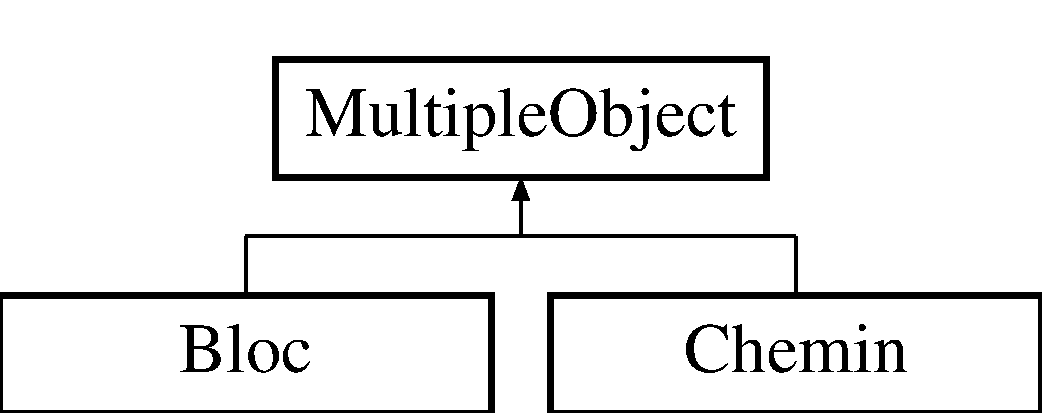
\includegraphics[height=2.000000cm]{classMultipleObject}
\end{center}
\end{figure}
\subsection*{Fonctions membres publiques}
\begin{DoxyCompactItemize}
\item 
virtual bool \hyperlink{classMultipleObject_aa5e743143bdedeb901c8e234162b3db1}{add} (int8\-\_\-t x, int8\-\_\-t y)=0
\item 
virtual bool \hyperlink{classMultipleObject_ad57dd5fec65953bbce399afdca475a4c}{remove} (int8\-\_\-t x, int8\-\_\-t y)=0
\item 
virtual bool \hyperlink{classMultipleObject_a1703b0c461708fbb6985e87624f4b17b}{has} (int8\-\_\-t x, int8\-\_\-t y)=0
\item 
virtual bool \hyperlink{classMultipleObject_a980acdfb99e25ec0d5e61396f60517c3}{clear} ()=0
\item 
virtual std\-::string \hyperlink{classMultipleObject_a5439a2ac4cc86c759ef1df8f6059947a}{to\-String} ()=0
\end{DoxyCompactItemize}


\subsection{Documentation des fonctions membres}
\hypertarget{classMultipleObject_aa5e743143bdedeb901c8e234162b3db1}{\index{Multiple\-Object@{Multiple\-Object}!add@{add}}
\index{add@{add}!MultipleObject@{Multiple\-Object}}
\subsubsection[{add}]{\setlength{\rightskip}{0pt plus 5cm}virtual bool Multiple\-Object\-::add (
\begin{DoxyParamCaption}
\item[{int8\-\_\-t}]{x, }
\item[{int8\-\_\-t}]{y}
\end{DoxyParamCaption}
)\hspace{0.3cm}{\ttfamily [pure virtual]}}}\label{classMultipleObject_aa5e743143bdedeb901c8e234162b3db1}


Implémenté dans \hyperlink{classBloc_a02db4c95699ce40e8ad671ef759ebdb7}{Bloc}, et \hyperlink{classChemin_a2ee7b6a34082453fbdf890a49017aead}{Chemin}.

\hypertarget{classMultipleObject_a980acdfb99e25ec0d5e61396f60517c3}{\index{Multiple\-Object@{Multiple\-Object}!clear@{clear}}
\index{clear@{clear}!MultipleObject@{Multiple\-Object}}
\subsubsection[{clear}]{\setlength{\rightskip}{0pt plus 5cm}virtual bool Multiple\-Object\-::clear (
\begin{DoxyParamCaption}
{}
\end{DoxyParamCaption}
)\hspace{0.3cm}{\ttfamily [pure virtual]}}}\label{classMultipleObject_a980acdfb99e25ec0d5e61396f60517c3}


Implémenté dans \hyperlink{classBloc_afa48be18bb2cd4e3240f4a165abef1c8}{Bloc}, et \hyperlink{classChemin_a67a8418164f0b2a4d1827e393ba859f7}{Chemin}.

\hypertarget{classMultipleObject_a1703b0c461708fbb6985e87624f4b17b}{\index{Multiple\-Object@{Multiple\-Object}!has@{has}}
\index{has@{has}!MultipleObject@{Multiple\-Object}}
\subsubsection[{has}]{\setlength{\rightskip}{0pt plus 5cm}virtual bool Multiple\-Object\-::has (
\begin{DoxyParamCaption}
\item[{int8\-\_\-t}]{x, }
\item[{int8\-\_\-t}]{y}
\end{DoxyParamCaption}
)\hspace{0.3cm}{\ttfamily [pure virtual]}}}\label{classMultipleObject_a1703b0c461708fbb6985e87624f4b17b}


Implémenté dans \hyperlink{classBloc_a03799c83e18411ab4ae4bf3e03aec975}{Bloc}, et \hyperlink{classChemin_aceccf541a2cdde27eb8f4bf541aff1b3}{Chemin}.

\hypertarget{classMultipleObject_ad57dd5fec65953bbce399afdca475a4c}{\index{Multiple\-Object@{Multiple\-Object}!remove@{remove}}
\index{remove@{remove}!MultipleObject@{Multiple\-Object}}
\subsubsection[{remove}]{\setlength{\rightskip}{0pt plus 5cm}virtual bool Multiple\-Object\-::remove (
\begin{DoxyParamCaption}
\item[{int8\-\_\-t}]{x, }
\item[{int8\-\_\-t}]{y}
\end{DoxyParamCaption}
)\hspace{0.3cm}{\ttfamily [pure virtual]}}}\label{classMultipleObject_ad57dd5fec65953bbce399afdca475a4c}


Implémenté dans \hyperlink{classBloc_a259248faed302444ba5424cdf6178681}{Bloc}, et \hyperlink{classChemin_a1ee3f200283c2c401ef0ffd5800d946c}{Chemin}.

\hypertarget{classMultipleObject_a5439a2ac4cc86c759ef1df8f6059947a}{\index{Multiple\-Object@{Multiple\-Object}!to\-String@{to\-String}}
\index{to\-String@{to\-String}!MultipleObject@{Multiple\-Object}}
\subsubsection[{to\-String}]{\setlength{\rightskip}{0pt plus 5cm}virtual std\-::string Multiple\-Object\-::to\-String (
\begin{DoxyParamCaption}
{}
\end{DoxyParamCaption}
)\hspace{0.3cm}{\ttfamily [pure virtual]}}}\label{classMultipleObject_a5439a2ac4cc86c759ef1df8f6059947a}


Implémenté dans \hyperlink{classBloc_a040af8a2aefc1acaa0e2d9bfc5943fa3}{Bloc}, et \hyperlink{classChemin_a3b1754233eb79fb9f7d119a42efbda3c}{Chemin}.



La documentation de cette classe a été générée à partir du fichier suivant \-:\begin{DoxyCompactItemize}
\item 
headers/abstract/\hyperlink{multipleobject_8h}{multipleobject.\-h}\end{DoxyCompactItemize}

\hypertarget{classPathFinding}{\section{Référence de la classe Path\-Finding}
\label{classPathFinding}\index{Path\-Finding@{Path\-Finding}}
}


{\ttfamily \#include $<$pathfinding.\-h$>$}

\subsection*{Fonctions membres publiques}
\begin{DoxyCompactItemize}
\item 
\hyperlink{classPathFinding_aff5b197409e0489e6df3c2366ee6f8cd}{Path\-Finding} (int8\-\_\-t $\ast$$\ast$matrice, int8\-\_\-t width\-\_\-scene, int8\-\_\-t height\-\_\-scene, std\-::pair$<$ int8\-\_\-t, int8\-\_\-t $>$ start, std\-::pair$<$ int8\-\_\-t, int8\-\_\-t $>$ end)
\item 
bool \hyperlink{classPathFinding_a2cb53ee646709c2367a6819d758ec7c3}{ever\-Parent} (\hyperlink{classCellule}{Cellule} $\ast$current, \hyperlink{classCellule}{Cellule} $\ast$parent)
\item 
bool \hyperlink{classPathFinding_a8d70d17f06400cdcd5787331d7be38e2}{has\-Possibility} ()
\item 
std\-::vector$<$ std\-::pair$<$ int8\-\_\-t, \\*
int8\-\_\-t $>$ $>$ $\ast$ \hyperlink{classPathFinding_aff1ca43a0ea5e4b9e5e188f165f08cd2}{get\-Chemin} ()
\item 
\hyperlink{classPathFinding_a0fc7389a32fa31a194a940a89f252bdb}{$\sim$\-Path\-Finding} ()
\end{DoxyCompactItemize}
\subsection*{Fonctions membres privées}
\begin{DoxyCompactItemize}
\item 
void \hyperlink{classPathFinding_addc7b9eb5682e0de46fd59c4a1319a86}{find\-Path} ()
\item 
\hyperlink{classCellule}{Cellule} $\ast$ \hyperlink{classPathFinding_a3817cc8f9d1604bf34a5a3b4f878b3da}{get\-Cellule} (int8\-\_\-t x, int8\-\_\-t y)
\item 
bool \hyperlink{classPathFinding_ad85b700719e73736e36d2548f950323a}{surrounded\-Blocs} (int8\-\_\-t x, int8\-\_\-t y, int8\-\_\-t $\ast$$\ast$matrice)
\end{DoxyCompactItemize}
\subsection*{Attributs privés}
\begin{DoxyCompactItemize}
\item 
\hyperlink{classCellule}{Cellule} $\ast$ \hyperlink{classPathFinding_ada148538e4a78dcc97f24ae74156abd4}{\-\_\-pathfinding}
\item 
std\-::vector$<$ std\-::pair$<$ int8\-\_\-t, \\*
int8\-\_\-t $>$ $>$ $\ast$ \hyperlink{classPathFinding_a1c1b4bc29b0f8a74f80d2601c83844aa}{list\-\_\-chemin\-Ok}
\item 
std\-::vector$<$ \hyperlink{classCellule}{Cellule} $\ast$ $>$ \hyperlink{classPathFinding_ae2eff9f0d9ffba2d88d405d10c34660a}{all\-\_\-cellules}
\item 
std\-::vector$<$ \hyperlink{classCellule}{Cellule} $\ast$ $>$ \hyperlink{classPathFinding_aac0f1388f79b45388470d634c909174e}{current\-\_\-list}
\item 
int8\-\_\-t \hyperlink{classPathFinding_a50f9513402ad1113678635c3eb9da62d}{width}
\item 
int8\-\_\-t \hyperlink{classPathFinding_a61e5643d7459d24b07306a6886348ca1}{height}
\item 
std\-::pair$<$ int8\-\_\-t, int8\-\_\-t $>$ \hyperlink{classPathFinding_a33dac4c9b17f5e6032bc0fc60e7a8249}{start\-\_\-coord}
\item 
std\-::pair$<$ int8\-\_\-t, int8\-\_\-t $>$ \hyperlink{classPathFinding_a7db7c62b00778fb60be8fdb10c471851}{end\-\_\-coord}
\end{DoxyCompactItemize}


\subsection{Documentation des constructeurs et destructeur}
\hypertarget{classPathFinding_aff5b197409e0489e6df3c2366ee6f8cd}{\index{Path\-Finding@{Path\-Finding}!Path\-Finding@{Path\-Finding}}
\index{Path\-Finding@{Path\-Finding}!PathFinding@{Path\-Finding}}
\subsubsection[{Path\-Finding}]{\setlength{\rightskip}{0pt plus 5cm}Path\-Finding\-::\-Path\-Finding (
\begin{DoxyParamCaption}
\item[{int8\-\_\-t $\ast$$\ast$}]{matrice, }
\item[{int8\-\_\-t}]{width\-\_\-scene, }
\item[{int8\-\_\-t}]{height\-\_\-scene, }
\item[{std\-::pair$<$ int8\-\_\-t, int8\-\_\-t $>$}]{start, }
\item[{std\-::pair$<$ int8\-\_\-t, int8\-\_\-t $>$}]{end}
\end{DoxyParamCaption}
)\hspace{0.3cm}{\ttfamily [inline]}}}\label{classPathFinding_aff5b197409e0489e6df3c2366ee6f8cd}


Références \-\_\-pathfinding, all\-\_\-cellules, B\-L\-O\-C\-\_\-\-D\-E\-F, current\-\_\-list, end\-\_\-coord, Cellule\-::everfind, find\-Path(), get\-Cellule(), height, list\-\_\-chemin\-Ok, Cellule\-::m\-\_\-\-P, start\-\_\-coord, surrounded\-Blocs(), et width.


\begin{DoxyCode}
29                                                                                       \{
30             \hyperlink{classPathFinding_a33dac4c9b17f5e6032bc0fc60e7a8249}{start\_coord} = start;
31             \hyperlink{classPathFinding_a7db7c62b00778fb60be8fdb10c471851}{end\_coord} = end;
32             \hyperlink{classPathFinding_a50f9513402ad1113678635c3eb9da62d}{width} = width\_scene;
33             \hyperlink{classPathFinding_a61e5643d7459d24b07306a6886348ca1}{height} = height\_scene;
34             \hyperlink{classPathFinding_ada148538e4a78dcc97f24ae74156abd4}{\_pathfinding} = \textcolor{keyword}{nullptr};
35             \textcolor{keywordflow}{if}(\hyperlink{classPathFinding_ad85b700719e73736e36d2548f950323a}{surroundedBlocs}(end.first, end.second, matrice) || 
      \hyperlink{classPathFinding_ad85b700719e73736e36d2548f950323a}{surroundedBlocs}(start.first, start.second, matrice))\{
36                 \textcolor{keywordflow}{return};
37             \}
38             \textcolor{keywordflow}{for}(int8\_t i\_width = 0; i\_width < width\_scene; ++i\_width)\{
39                 \textcolor{keywordflow}{for}(int8\_t i\_height= 0; i\_height < height\_scene; ++i\_height)\{
40                     \textcolor{keywordtype}{bool} isbloc = (matrice[i\_width][i\_height] == \hyperlink{definition_8h_a4d275339ef3ddec11c63b8b925b5b358}{BLOC\_DEF});
41                     \hyperlink{classPathFinding_ae2eff9f0d9ffba2d88d405d10c34660a}{all\_cellules}.push\_back(\textcolor{keyword}{new} \hyperlink{classCellule}{Cellule}(i\_width, i\_height, isbloc));
42                 \}
43             \}
44             \hyperlink{classCellule}{Cellule} *firstCell = \hyperlink{classPathFinding_a3817cc8f9d1604bf34a5a3b4f878b3da}{getCellule}(start.first, start.second);
45             firstCell->\hyperlink{classCellule_af7cb9856701ea3e423f58b09bb7dfdbd}{m\_P} = 0;
46             firstCell->\hyperlink{classCellule_a9c368e6fb89c5ea1e31b810207eca9ee}{everfind} = \textcolor{keyword}{true};
47             \hyperlink{classPathFinding_aac0f1388f79b45388470d634c909174e}{current\_list}.push\_back(firstCell);
48             \hyperlink{classPathFinding_addc7b9eb5682e0de46fd59c4a1319a86}{findPath}();
49             \hyperlink{classPathFinding_a1c1b4bc29b0f8a74f80d2601c83844aa}{list\_cheminOk} = \textcolor{keyword}{new} std::vector<std::pair<int8\_t, int8\_t>>();
50             \hyperlink{classPathFinding_a1c1b4bc29b0f8a74f80d2601c83844aa}{list\_cheminOk}->reserve(width\_scene*(width\_scene/2));
51         \}
\end{DoxyCode}
\hypertarget{classPathFinding_a0fc7389a32fa31a194a940a89f252bdb}{\index{Path\-Finding@{Path\-Finding}!$\sim$\-Path\-Finding@{$\sim$\-Path\-Finding}}
\index{$\sim$\-Path\-Finding@{$\sim$\-Path\-Finding}!PathFinding@{Path\-Finding}}
\subsubsection[{$\sim$\-Path\-Finding}]{\setlength{\rightskip}{0pt plus 5cm}Path\-Finding\-::$\sim$\-Path\-Finding (
\begin{DoxyParamCaption}
{}
\end{DoxyParamCaption}
)\hspace{0.3cm}{\ttfamily [inline]}}}\label{classPathFinding_a0fc7389a32fa31a194a940a89f252bdb}


Références \-\_\-pathfinding, all\-\_\-cellules, current\-\_\-list, et list\-\_\-chemin\-Ok.


\begin{DoxyCode}
111                   \{
112         \textcolor{keyword}{delete} \hyperlink{classPathFinding_ada148538e4a78dcc97f24ae74156abd4}{\_pathfinding};
113         \hyperlink{classPathFinding_ada148538e4a78dcc97f24ae74156abd4}{\_pathfinding} = \textcolor{keyword}{nullptr};
114         \textcolor{keyword}{delete} []\hyperlink{classPathFinding_a1c1b4bc29b0f8a74f80d2601c83844aa}{list\_cheminOk};
115         \hyperlink{classPathFinding_a1c1b4bc29b0f8a74f80d2601c83844aa}{list\_cheminOk} = \textcolor{keyword}{nullptr};
116         \textcolor{keywordflow}{for}(uint8\_t i=0; i<\hyperlink{classPathFinding_ae2eff9f0d9ffba2d88d405d10c34660a}{all\_cellules}.size(); ++i)\{
117             \textcolor{keyword}{delete} \hyperlink{classPathFinding_ae2eff9f0d9ffba2d88d405d10c34660a}{all\_cellules}[i];
118             \hyperlink{classPathFinding_ae2eff9f0d9ffba2d88d405d10c34660a}{all\_cellules}[i] = \textcolor{keyword}{nullptr};
119         \}
120         \textcolor{keywordflow}{for}(uint8\_t i=0; i<\hyperlink{classPathFinding_aac0f1388f79b45388470d634c909174e}{current\_list}.size(); ++i)\{
121             \textcolor{keyword}{delete} \hyperlink{classPathFinding_aac0f1388f79b45388470d634c909174e}{current\_list}[i];
122             \hyperlink{classPathFinding_aac0f1388f79b45388470d634c909174e}{current\_list}[i] = \textcolor{keyword}{nullptr};
123         \}
124         
125     \}
\end{DoxyCode}


\subsection{Documentation des fonctions membres}
\hypertarget{classPathFinding_a2cb53ee646709c2367a6819d758ec7c3}{\index{Path\-Finding@{Path\-Finding}!ever\-Parent@{ever\-Parent}}
\index{ever\-Parent@{ever\-Parent}!PathFinding@{Path\-Finding}}
\subsubsection[{ever\-Parent}]{\setlength{\rightskip}{0pt plus 5cm}bool Path\-Finding\-::ever\-Parent (
\begin{DoxyParamCaption}
\item[{{\bf Cellule} $\ast$}]{current, }
\item[{{\bf Cellule} $\ast$}]{parent}
\end{DoxyParamCaption}
)\hspace{0.3cm}{\ttfamily [inline]}}}\label{classPathFinding_a2cb53ee646709c2367a6819d758ec7c3}


Références Cellule\-::m\-\_\-parent.



Référencé par find\-Path().


\begin{DoxyCode}
53                                                       \{
54         \hyperlink{classCellule}{Cellule} *\_current = current;
55         \textcolor{keywordflow}{if}(current->\hyperlink{classCellule_a3f4117017976fde614e72d38ea10d734}{m\_parent} == \textcolor{keyword}{nullptr})
56             \textcolor{keywordflow}{return} \textcolor{keyword}{false};
57         \textcolor{keywordflow}{while}(\_current != \textcolor{keyword}{nullptr})\{
58             \textcolor{keywordflow}{if}(\_current == parent)\{
59                 \textcolor{keywordflow}{return} \textcolor{keyword}{true};
60             \}\textcolor{keywordflow}{else}\{
61                 \_current = \_current->\hyperlink{classCellule_a3f4117017976fde614e72d38ea10d734}{m\_parent};
62             \}
63         \}
64         \textcolor{keywordflow}{return} \textcolor{keyword}{false};
65     \}
\end{DoxyCode}
\hypertarget{classPathFinding_addc7b9eb5682e0de46fd59c4a1319a86}{\index{Path\-Finding@{Path\-Finding}!find\-Path@{find\-Path}}
\index{find\-Path@{find\-Path}!PathFinding@{Path\-Finding}}
\subsubsection[{find\-Path}]{\setlength{\rightskip}{0pt plus 5cm}void Path\-Finding\-::find\-Path (
\begin{DoxyParamCaption}
{}
\end{DoxyParamCaption}
)\hspace{0.3cm}{\ttfamily [inline]}, {\ttfamily [private]}}}\label{classPathFinding_addc7b9eb5682e0de46fd59c4a1319a86}


Références \-\_\-pathfinding, current\-\_\-list, end\-\_\-coord, ever\-Parent(), get\-Cellule(), Cellule\-::get\-Coord(), Cellule\-::m\-\_\-\-P, et Cellule\-::m\-\_\-parent.



Référencé par Path\-Finding().


\begin{DoxyCode}
151                    \{
152         \hyperlink{classPathFinding_ada148538e4a78dcc97f24ae74156abd4}{\_pathfinding} = \textcolor{keyword}{nullptr};
153         \textcolor{keywordflow}{if}(\hyperlink{classPathFinding_aac0f1388f79b45388470d634c909174e}{current\_list}.size() == 0)
154             \textcolor{keywordflow}{return};
155         std::vector<Cellule*> actuel\_list = \hyperlink{classPathFinding_aac0f1388f79b45388470d634c909174e}{current\_list};
156         \hyperlink{classPathFinding_aac0f1388f79b45388470d634c909174e}{current\_list}.clear();
157         \textcolor{keywordflow}{for}(uint8\_t \hyperlink{server_8cpp_a30792c4b007e8273d3832fe2d5e70987}{index}=0; \hyperlink{server_8cpp_a30792c4b007e8273d3832fe2d5e70987}{index}<(uint8\_t)actuel\_list.size(); ++
      \hyperlink{server_8cpp_a30792c4b007e8273d3832fe2d5e70987}{index})\{
158             \hyperlink{classCellule}{Cellule}* \_currentCell = actuel\_list.at(\hyperlink{server_8cpp_a30792c4b007e8273d3832fe2d5e70987}{index});
159             uint16\_t newP = \_currentCell->\hyperlink{classCellule_af7cb9856701ea3e423f58b09bb7dfdbd}{m\_P}+10;
160             \hyperlink{classCellule}{Cellule}* down = \hyperlink{classPathFinding_a3817cc8f9d1604bf34a5a3b4f878b3da}{getCellule}(\_currentCell->\hyperlink{classCellule_a50698c84ba5a043a148a594552189427}{getCoord}().first + 1, 
      \_currentCell->\hyperlink{classCellule_a50698c84ba5a043a148a594552189427}{getCoord}().second);
161             \hyperlink{classCellule}{Cellule}* up = \hyperlink{classPathFinding_a3817cc8f9d1604bf34a5a3b4f878b3da}{getCellule}(\_currentCell->\hyperlink{classCellule_a50698c84ba5a043a148a594552189427}{getCoord}().first - 1, 
      \_currentCell->\hyperlink{classCellule_a50698c84ba5a043a148a594552189427}{getCoord}().second);
162             \hyperlink{classCellule}{Cellule}* right = \hyperlink{classPathFinding_a3817cc8f9d1604bf34a5a3b4f878b3da}{getCellule}(\_currentCell->\hyperlink{classCellule_a50698c84ba5a043a148a594552189427}{getCoord}().first, 
      \_currentCell->\hyperlink{classCellule_a50698c84ba5a043a148a594552189427}{getCoord}().second + 1);
163             \hyperlink{classCellule}{Cellule}* left = \hyperlink{classPathFinding_a3817cc8f9d1604bf34a5a3b4f878b3da}{getCellule}(\_currentCell->\hyperlink{classCellule_a50698c84ba5a043a148a594552189427}{getCoord}().first, 
      \_currentCell->\hyperlink{classCellule_a50698c84ba5a043a148a594552189427}{getCoord}().second - 1);
164             \textcolor{comment}{//}
165             \hyperlink{classCellule}{Cellule}* a1 = \hyperlink{classPathFinding_a3817cc8f9d1604bf34a5a3b4f878b3da}{getCellule}(\_currentCell->\hyperlink{classCellule_a50698c84ba5a043a148a594552189427}{getCoord}().first - 1, 
      \_currentCell->\hyperlink{classCellule_a50698c84ba5a043a148a594552189427}{getCoord}().second - 2);
166             \hyperlink{classCellule}{Cellule}* d1 = \hyperlink{classPathFinding_a3817cc8f9d1604bf34a5a3b4f878b3da}{getCellule}(\_currentCell->\hyperlink{classCellule_a50698c84ba5a043a148a594552189427}{getCoord}().first, \_currentCell
      ->\hyperlink{classCellule_a50698c84ba5a043a148a594552189427}{getCoord}().second - 2);
167             \hyperlink{classCellule}{Cellule}* g2 = \hyperlink{classPathFinding_a3817cc8f9d1604bf34a5a3b4f878b3da}{getCellule}(\_currentCell->\hyperlink{classCellule_a50698c84ba5a043a148a594552189427}{getCoord}().first + 1, 
      \_currentCell->\hyperlink{classCellule_a50698c84ba5a043a148a594552189427}{getCoord}().second - 2);
168             \hyperlink{classCellule}{Cellule}* g1 = \hyperlink{classPathFinding_a3817cc8f9d1604bf34a5a3b4f878b3da}{getCellule}(\_currentCell->\hyperlink{classCellule_a50698c84ba5a043a148a594552189427}{getCoord}().first + 2, 
      \_currentCell->\hyperlink{classCellule_a50698c84ba5a043a148a594552189427}{getCoord}().second -1);
169             \hyperlink{classCellule}{Cellule}* h1 = \hyperlink{classPathFinding_a3817cc8f9d1604bf34a5a3b4f878b3da}{getCellule}(\_currentCell->\hyperlink{classCellule_a50698c84ba5a043a148a594552189427}{getCoord}().first + 2, 
      \_currentCell->\hyperlink{classCellule_a50698c84ba5a043a148a594552189427}{getCoord}().second);
170             \hyperlink{classCellule}{Cellule}* i1 = \hyperlink{classPathFinding_a3817cc8f9d1604bf34a5a3b4f878b3da}{getCellule}(\_currentCell->\hyperlink{classCellule_a50698c84ba5a043a148a594552189427}{getCoord}().first + 2, 
      \_currentCell->\hyperlink{classCellule_a50698c84ba5a043a148a594552189427}{getCoord}().second + 1);
171             \hyperlink{classCellule}{Cellule}* i2 = \hyperlink{classPathFinding_a3817cc8f9d1604bf34a5a3b4f878b3da}{getCellule}(\_currentCell->\hyperlink{classCellule_a50698c84ba5a043a148a594552189427}{getCoord}().first + 1, 
      \_currentCell->\hyperlink{classCellule_a50698c84ba5a043a148a594552189427}{getCoord}().second + 2);
172             \hyperlink{classCellule}{Cellule}* f1 = \hyperlink{classPathFinding_a3817cc8f9d1604bf34a5a3b4f878b3da}{getCellule}(\_currentCell->\hyperlink{classCellule_a50698c84ba5a043a148a594552189427}{getCoord}().first, \_currentCell
      ->\hyperlink{classCellule_a50698c84ba5a043a148a594552189427}{getCoord}().second + 2);
173             \hyperlink{classCellule}{Cellule}* c2 = \hyperlink{classPathFinding_a3817cc8f9d1604bf34a5a3b4f878b3da}{getCellule}(\_currentCell->\hyperlink{classCellule_a50698c84ba5a043a148a594552189427}{getCoord}().first - 1, 
      \_currentCell->\hyperlink{classCellule_a50698c84ba5a043a148a594552189427}{getCoord}().second + 2);
174             \hyperlink{classCellule}{Cellule}* c1 = \hyperlink{classPathFinding_a3817cc8f9d1604bf34a5a3b4f878b3da}{getCellule}(\_currentCell->\hyperlink{classCellule_a50698c84ba5a043a148a594552189427}{getCoord}().first - 2, 
      \_currentCell->\hyperlink{classCellule_a50698c84ba5a043a148a594552189427}{getCoord}().second +1);
175             \hyperlink{classCellule}{Cellule}* b1 = \hyperlink{classPathFinding_a3817cc8f9d1604bf34a5a3b4f878b3da}{getCellule}(\_currentCell->\hyperlink{classCellule_a50698c84ba5a043a148a594552189427}{getCoord}().first - 2, 
      \_currentCell->\hyperlink{classCellule_a50698c84ba5a043a148a594552189427}{getCoord}().second);
176             \hyperlink{classCellule}{Cellule}* a2 = \hyperlink{classPathFinding_a3817cc8f9d1604bf34a5a3b4f878b3da}{getCellule}(\_currentCell->\hyperlink{classCellule_a50698c84ba5a043a148a594552189427}{getCoord}().first - 2, 
      \_currentCell->\hyperlink{classCellule_a50698c84ba5a043a148a594552189427}{getCoord}().second -1);
177 
178             \textcolor{keywordflow}{if}(g1 != \textcolor{keyword}{nullptr} && h1 != \textcolor{keyword}{nullptr} && i1 != \textcolor{keyword}{nullptr} && down->\hyperlink{classCellule_a3f4117017976fde614e72d38ea10d734}{m\_parent} != \_currentCell)\{
179                 \textcolor{keywordflow}{if}(!g1->isBloc() && !h1->isBloc() && !i1->isBloc())\{
180                     \textcolor{keywordflow}{if}(newP < down->m\_P && !\hyperlink{classPathFinding_a2cb53ee646709c2367a6819d758ec7c3}{everParent}(\_currentCell->
      \hyperlink{classCellule_a3f4117017976fde614e72d38ea10d734}{m\_parent}, down))\{
181                         down->\hyperlink{classCellule_a3f4117017976fde614e72d38ea10d734}{m\_parent} = \_currentCell;
182                         down->\hyperlink{classCellule_af7cb9856701ea3e423f58b09bb7dfdbd}{m\_P} = newP;
183                         \hyperlink{classPathFinding_aac0f1388f79b45388470d634c909174e}{current\_list}.push\_back(down);
184                     \}
185                     \textcolor{keywordflow}{if}(down->\hyperlink{classCellule_a50698c84ba5a043a148a594552189427}{getCoord}().first == \hyperlink{classPathFinding_a7db7c62b00778fb60be8fdb10c471851}{end\_coord}.first && down->
      \hyperlink{classCellule_a50698c84ba5a043a148a594552189427}{getCoord}().second == \hyperlink{classPathFinding_a7db7c62b00778fb60be8fdb10c471851}{end\_coord}.second)\{
186                         \hyperlink{classPathFinding_ada148538e4a78dcc97f24ae74156abd4}{\_pathfinding} = \_currentCell;
187                         \textcolor{keywordflow}{break};
188                     \}
189                 \}
190             \}
191             \textcolor{keywordflow}{if}(a2 != \textcolor{keyword}{nullptr} && b1 != \textcolor{keyword}{nullptr} && c1 != \textcolor{keyword}{nullptr} && up->m\_parent != \_currentCell)\{
192                 \textcolor{keywordflow}{if}(!a2->isBloc() && !b1->isBloc() && !c1->isBloc())\{
193                     \textcolor{keywordflow}{if}(newP < up->m\_P && !\hyperlink{classPathFinding_a2cb53ee646709c2367a6819d758ec7c3}{everParent}(\_currentCell, up))\{
194                         up->\hyperlink{classCellule_a3f4117017976fde614e72d38ea10d734}{m\_parent} = \_currentCell;
195                         up->\hyperlink{classCellule_af7cb9856701ea3e423f58b09bb7dfdbd}{m\_P} = newP;
196                         \hyperlink{classPathFinding_aac0f1388f79b45388470d634c909174e}{current\_list}.push\_back(up);
197                     \}
198                 \}
199                 \textcolor{keywordflow}{if}(up->getCoord().first == \hyperlink{classPathFinding_a7db7c62b00778fb60be8fdb10c471851}{end\_coord}.first && up->getCoord().second == 
      \hyperlink{classPathFinding_a7db7c62b00778fb60be8fdb10c471851}{end\_coord}.second)\{
200                     \hyperlink{classPathFinding_ada148538e4a78dcc97f24ae74156abd4}{\_pathfinding} = \_currentCell;
201                     \textcolor{keywordflow}{break};
202                 \}
203             \}
204             \textcolor{keywordflow}{if}(a1 != \textcolor{keyword}{nullptr} && d1 != \textcolor{keyword}{nullptr} && g2 != \textcolor{keyword}{nullptr} && left->m\_parent != \_currentCell)\{
205                 \textcolor{keywordflow}{if}(!a1->isBloc() && !d1->isBloc() && !g2->isBloc())\{
206                     \textcolor{keywordflow}{if}(newP < left->m\_P && !\hyperlink{classPathFinding_a2cb53ee646709c2367a6819d758ec7c3}{everParent}(\_currentCell->
      \hyperlink{classCellule_a3f4117017976fde614e72d38ea10d734}{m\_parent}, left))\{
207                         left->\hyperlink{classCellule_a3f4117017976fde614e72d38ea10d734}{m\_parent} = \_currentCell;
208                         left->\hyperlink{classCellule_af7cb9856701ea3e423f58b09bb7dfdbd}{m\_P} = newP;
209                         \hyperlink{classPathFinding_aac0f1388f79b45388470d634c909174e}{current\_list}.push\_back(left);
210                     \}
211                 \}
212                 \textcolor{keywordflow}{if}(left->getCoord().first == \hyperlink{classPathFinding_a7db7c62b00778fb60be8fdb10c471851}{end\_coord}.first && left->getCoord().second == 
      \hyperlink{classPathFinding_a7db7c62b00778fb60be8fdb10c471851}{end\_coord}.second)\{
213                     \hyperlink{classPathFinding_ada148538e4a78dcc97f24ae74156abd4}{\_pathfinding} = \_currentCell;
214                     \textcolor{keywordflow}{break};
215                 \}
216             \}
217             \textcolor{keywordflow}{if}(c2 != \textcolor{keyword}{nullptr} && f1 !=\textcolor{keyword}{nullptr} && i2 != \textcolor{keyword}{nullptr} && right->m\_parent != \_currentCell)\{
218                 \textcolor{keywordflow}{if}(!c2->isBloc() && !f1->isBloc() && !i2->isBloc())\{
219                     \textcolor{keywordflow}{if}(newP < right->m\_P && !\hyperlink{classPathFinding_a2cb53ee646709c2367a6819d758ec7c3}{everParent}(\_currentCell->
      \hyperlink{classCellule_a3f4117017976fde614e72d38ea10d734}{m\_parent}, right))\{
220                         right->\hyperlink{classCellule_a3f4117017976fde614e72d38ea10d734}{m\_parent} = \_currentCell;
221                         right->\hyperlink{classCellule_af7cb9856701ea3e423f58b09bb7dfdbd}{m\_P} = newP;
222                         \hyperlink{classPathFinding_aac0f1388f79b45388470d634c909174e}{current\_list}.push\_back(right);
223                     \}
224                 \}
225                 \textcolor{keywordflow}{if}(right->getCoord().first == \hyperlink{classPathFinding_a7db7c62b00778fb60be8fdb10c471851}{end\_coord}.first && right->getCoord().second == 
      \hyperlink{classPathFinding_a7db7c62b00778fb60be8fdb10c471851}{end\_coord}.second)\{
226                     \hyperlink{classPathFinding_ada148538e4a78dcc97f24ae74156abd4}{\_pathfinding} = \_currentCell;
227                     \textcolor{keywordflow}{break};
228                 \}
229             \}
230         \}
231         \textcolor{keywordflow}{if}(\hyperlink{classPathFinding_ada148538e4a78dcc97f24ae74156abd4}{\_pathfinding} == \textcolor{keyword}{nullptr})\{
232             \hyperlink{classPathFinding_addc7b9eb5682e0de46fd59c4a1319a86}{findPath}();
233         \} 
234         \textcolor{keywordflow}{return};
235     \}
\end{DoxyCode}
\hypertarget{classPathFinding_a3817cc8f9d1604bf34a5a3b4f878b3da}{\index{Path\-Finding@{Path\-Finding}!get\-Cellule@{get\-Cellule}}
\index{get\-Cellule@{get\-Cellule}!PathFinding@{Path\-Finding}}
\subsubsection[{get\-Cellule}]{\setlength{\rightskip}{0pt plus 5cm}{\bf Cellule}$\ast$ Path\-Finding\-::get\-Cellule (
\begin{DoxyParamCaption}
\item[{int8\-\_\-t}]{x, }
\item[{int8\-\_\-t}]{y}
\end{DoxyParamCaption}
)\hspace{0.3cm}{\ttfamily [inline]}, {\ttfamily [private]}}}\label{classPathFinding_a3817cc8f9d1604bf34a5a3b4f878b3da}


Références all\-\_\-cellules, height, et width.



Référencé par find\-Path(), et Path\-Finding().


\begin{DoxyCode}
246                                            \{
247         \textcolor{keywordflow}{if}(x < 0 || y < 0)
248             \textcolor{keywordflow}{return} \textcolor{keyword}{nullptr};
249         \textcolor{keywordflow}{if}(x >= \hyperlink{classPathFinding_a50f9513402ad1113678635c3eb9da62d}{width} || y >= \hyperlink{classPathFinding_a61e5643d7459d24b07306a6886348ca1}{height})
250             \textcolor{keywordflow}{return} \textcolor{keyword}{nullptr};
251         uint16\_t \hyperlink{server_8cpp_a30792c4b007e8273d3832fe2d5e70987}{index} = (\hyperlink{classPathFinding_a61e5643d7459d24b07306a6886348ca1}{height}*x) + y;
252         \textcolor{keywordflow}{if}(\hyperlink{classPathFinding_ae2eff9f0d9ffba2d88d405d10c34660a}{all\_cellules}.size() > \hyperlink{server_8cpp_a30792c4b007e8273d3832fe2d5e70987}{index})
253             \textcolor{keywordflow}{return} \hyperlink{classPathFinding_ae2eff9f0d9ffba2d88d405d10c34660a}{all\_cellules}.at(index);
254         \textcolor{keywordflow}{return} \textcolor{keyword}{nullptr};
255     \}
\end{DoxyCode}
\hypertarget{classPathFinding_aff1ca43a0ea5e4b9e5e188f165f08cd2}{\index{Path\-Finding@{Path\-Finding}!get\-Chemin@{get\-Chemin}}
\index{get\-Chemin@{get\-Chemin}!PathFinding@{Path\-Finding}}
\subsubsection[{get\-Chemin}]{\setlength{\rightskip}{0pt plus 5cm}std\-::vector$<$std\-::pair$<$int8\-\_\-t, int8\-\_\-t$>$ $>$$\ast$ Path\-Finding\-::get\-Chemin (
\begin{DoxyParamCaption}
{}
\end{DoxyParamCaption}
)\hspace{0.3cm}{\ttfamily [inline]}}}\label{classPathFinding_aff1ca43a0ea5e4b9e5e188f165f08cd2}


Références \-\_\-pathfinding, Cellule\-::everfind, Cellule\-::get\-Coord(), list\-\_\-chemin\-Ok, Cellule\-::m\-\_\-parent, et start\-\_\-coord.



Référencé par Core\-::pathfinding(), et unitest\-\_\-pathfinding().


\begin{DoxyCode}
84                                                    \{
85         \hyperlink{classPathFinding_a1c1b4bc29b0f8a74f80d2601c83844aa}{list\_cheminOk}->clear();
86         \hyperlink{classCellule}{Cellule} *current = \hyperlink{classPathFinding_ada148538e4a78dcc97f24ae74156abd4}{\_pathfinding};
87         \textcolor{keywordflow}{while}(\textcolor{keyword}{true})\{
88             \textcolor{keywordflow}{if}(current == \textcolor{keyword}{nullptr})
89                 \textcolor{keywordflow}{break};
90             \textcolor{keywordflow}{if}(current->\hyperlink{classCellule_a50698c84ba5a043a148a594552189427}{getCoord}() != \hyperlink{classPathFinding_a33dac4c9b17f5e6032bc0fc60e7a8249}{start\_coord})
91                 \hyperlink{classPathFinding_a1c1b4bc29b0f8a74f80d2601c83844aa}{list\_cheminOk}->push\_back(current->\hyperlink{classCellule_a50698c84ba5a043a148a594552189427}{getCoord}());
92             \textcolor{keywordflow}{if}(current->\hyperlink{classCellule_a3f4117017976fde614e72d38ea10d734}{m\_parent} != \textcolor{keyword}{nullptr} && !current->\hyperlink{classCellule_a3f4117017976fde614e72d38ea10d734}{m\_parent}->
      \hyperlink{classCellule_a9c368e6fb89c5ea1e31b810207eca9ee}{everfind})\{
93                 current = current->\hyperlink{classCellule_a3f4117017976fde614e72d38ea10d734}{m\_parent};
94                 current->\hyperlink{classCellule_a9c368e6fb89c5ea1e31b810207eca9ee}{everfind} = \textcolor{keyword}{true};
95             \}\textcolor{keywordflow}{else}\{
96                 \textcolor{keywordflow}{break};
97             \}
98         \}
99         \textcolor{keywordflow}{if}(current != \textcolor{keyword}{nullptr})
100             \hyperlink{classPathFinding_a1c1b4bc29b0f8a74f80d2601c83844aa}{list\_cheminOk}->push\_back(current->\hyperlink{classCellule_a50698c84ba5a043a148a594552189427}{getCoord}());
101         \textcolor{comment}{//list\_cheminOk->pop\_back();}
102         \textcolor{keywordflow}{return} \hyperlink{classPathFinding_a1c1b4bc29b0f8a74f80d2601c83844aa}{list\_cheminOk};
103     \}
\end{DoxyCode}
\hypertarget{classPathFinding_a8d70d17f06400cdcd5787331d7be38e2}{\index{Path\-Finding@{Path\-Finding}!has\-Possibility@{has\-Possibility}}
\index{has\-Possibility@{has\-Possibility}!PathFinding@{Path\-Finding}}
\subsubsection[{has\-Possibility}]{\setlength{\rightskip}{0pt plus 5cm}bool Path\-Finding\-::has\-Possibility (
\begin{DoxyParamCaption}
{}
\end{DoxyParamCaption}
)\hspace{0.3cm}{\ttfamily [inline]}}}\label{classPathFinding_a8d70d17f06400cdcd5787331d7be38e2}


Références \-\_\-pathfinding.



Référencé par Core\-::pathfinding(), et unitest\-\_\-pathfinding().


\begin{DoxyCode}
73                          \{
74         \textcolor{keywordflow}{return} \hyperlink{classPathFinding_ada148538e4a78dcc97f24ae74156abd4}{\_pathfinding} != \textcolor{keyword}{nullptr};
75     \}
\end{DoxyCode}
\hypertarget{classPathFinding_ad85b700719e73736e36d2548f950323a}{\index{Path\-Finding@{Path\-Finding}!surrounded\-Blocs@{surrounded\-Blocs}}
\index{surrounded\-Blocs@{surrounded\-Blocs}!PathFinding@{Path\-Finding}}
\subsubsection[{surrounded\-Blocs}]{\setlength{\rightskip}{0pt plus 5cm}bool Path\-Finding\-::surrounded\-Blocs (
\begin{DoxyParamCaption}
\item[{int8\-\_\-t}]{x, }
\item[{int8\-\_\-t}]{y, }
\item[{int8\-\_\-t $\ast$$\ast$}]{matrice}
\end{DoxyParamCaption}
)\hspace{0.3cm}{\ttfamily [inline]}, {\ttfamily [private]}}}\label{classPathFinding_ad85b700719e73736e36d2548f950323a}


Références height, et width.



Référencé par Path\-Finding().


\begin{DoxyCode}
268                                                               \{
269         \textcolor{keywordflow}{if}(x == 0)\{
270             \textcolor{keywordflow}{if}(matrice[x+1][y] == 0)
271                 \textcolor{keywordflow}{return} \textcolor{keyword}{false};
272         \}
273         \textcolor{keywordflow}{if}(y == 0)\{
274             \textcolor{keywordflow}{if}(matrice[x][y+1] == 0)
275                 \textcolor{keywordflow}{return} \textcolor{keyword}{false};
276         \}
277         \textcolor{keywordflow}{if}(0 < x && x<\hyperlink{classPathFinding_a50f9513402ad1113678635c3eb9da62d}{width}-1)\{
278             \textcolor{keywordflow}{if}(matrice[x+1][y] == 0 || matrice[x-1][y] == 0)
279                 \textcolor{keywordflow}{return} \textcolor{keyword}{false};
280         \}
281         \textcolor{keywordflow}{if}(0 < y && y<\hyperlink{classPathFinding_a61e5643d7459d24b07306a6886348ca1}{height}-1)\{
282             \textcolor{keywordflow}{if}(matrice[x][y+1] == 0 || matrice[x][y-1] == 0)
283                 \textcolor{keywordflow}{return} \textcolor{keyword}{false};
284         \}
285         \textcolor{keywordflow}{if}(x == \hyperlink{classPathFinding_a50f9513402ad1113678635c3eb9da62d}{width}-1)\{
286             \textcolor{keywordflow}{if}(matrice[x-1][y] == 0)
287                 \textcolor{keywordflow}{return} \textcolor{keyword}{false};
288         \}
289         \textcolor{keywordflow}{if}(y == \hyperlink{classPathFinding_a61e5643d7459d24b07306a6886348ca1}{height}-1)\{
290             \textcolor{keywordflow}{if}(matrice[x][y-1] == 0)
291                 \textcolor{keywordflow}{return} \textcolor{keyword}{false};
292         \}
293         \textcolor{keywordflow}{return} \textcolor{keyword}{true};
294     \}
\end{DoxyCode}


\subsection{Documentation des données membres}
\hypertarget{classPathFinding_ada148538e4a78dcc97f24ae74156abd4}{\index{Path\-Finding@{Path\-Finding}!\-\_\-pathfinding@{\-\_\-pathfinding}}
\index{\-\_\-pathfinding@{\-\_\-pathfinding}!PathFinding@{Path\-Finding}}
\subsubsection[{\-\_\-pathfinding}]{\setlength{\rightskip}{0pt plus 5cm}{\bf Cellule}$\ast$ Path\-Finding\-::\-\_\-pathfinding\hspace{0.3cm}{\ttfamily [private]}}}\label{classPathFinding_ada148538e4a78dcc97f24ae74156abd4}


Référencé par find\-Path(), get\-Chemin(), has\-Possibility(), Path\-Finding(), et $\sim$\-Path\-Finding().

\hypertarget{classPathFinding_ae2eff9f0d9ffba2d88d405d10c34660a}{\index{Path\-Finding@{Path\-Finding}!all\-\_\-cellules@{all\-\_\-cellules}}
\index{all\-\_\-cellules@{all\-\_\-cellules}!PathFinding@{Path\-Finding}}
\subsubsection[{all\-\_\-cellules}]{\setlength{\rightskip}{0pt plus 5cm}std\-::vector$<${\bf Cellule}$\ast$$>$ Path\-Finding\-::all\-\_\-cellules\hspace{0.3cm}{\ttfamily [private]}}}\label{classPathFinding_ae2eff9f0d9ffba2d88d405d10c34660a}


Référencé par get\-Cellule(), Path\-Finding(), et $\sim$\-Path\-Finding().

\hypertarget{classPathFinding_aac0f1388f79b45388470d634c909174e}{\index{Path\-Finding@{Path\-Finding}!current\-\_\-list@{current\-\_\-list}}
\index{current\-\_\-list@{current\-\_\-list}!PathFinding@{Path\-Finding}}
\subsubsection[{current\-\_\-list}]{\setlength{\rightskip}{0pt plus 5cm}std\-::vector$<${\bf Cellule}$\ast$$>$ Path\-Finding\-::current\-\_\-list\hspace{0.3cm}{\ttfamily [private]}}}\label{classPathFinding_aac0f1388f79b45388470d634c909174e}


Référencé par find\-Path(), Path\-Finding(), et $\sim$\-Path\-Finding().

\hypertarget{classPathFinding_a7db7c62b00778fb60be8fdb10c471851}{\index{Path\-Finding@{Path\-Finding}!end\-\_\-coord@{end\-\_\-coord}}
\index{end\-\_\-coord@{end\-\_\-coord}!PathFinding@{Path\-Finding}}
\subsubsection[{end\-\_\-coord}]{\setlength{\rightskip}{0pt plus 5cm}std\-::pair$<$int8\-\_\-t, int8\-\_\-t$>$ Path\-Finding\-::end\-\_\-coord\hspace{0.3cm}{\ttfamily [private]}}}\label{classPathFinding_a7db7c62b00778fb60be8fdb10c471851}


Référencé par find\-Path(), et Path\-Finding().

\hypertarget{classPathFinding_a61e5643d7459d24b07306a6886348ca1}{\index{Path\-Finding@{Path\-Finding}!height@{height}}
\index{height@{height}!PathFinding@{Path\-Finding}}
\subsubsection[{height}]{\setlength{\rightskip}{0pt plus 5cm}int8\-\_\-t Path\-Finding\-::height\hspace{0.3cm}{\ttfamily [private]}}}\label{classPathFinding_a61e5643d7459d24b07306a6886348ca1}


Référencé par get\-Cellule(), Path\-Finding(), et surrounded\-Blocs().

\hypertarget{classPathFinding_a1c1b4bc29b0f8a74f80d2601c83844aa}{\index{Path\-Finding@{Path\-Finding}!list\-\_\-chemin\-Ok@{list\-\_\-chemin\-Ok}}
\index{list\-\_\-chemin\-Ok@{list\-\_\-chemin\-Ok}!PathFinding@{Path\-Finding}}
\subsubsection[{list\-\_\-chemin\-Ok}]{\setlength{\rightskip}{0pt plus 5cm}std\-::vector$<$std\-::pair$<$int8\-\_\-t,int8\-\_\-t$>$ $>$$\ast$ Path\-Finding\-::list\-\_\-chemin\-Ok\hspace{0.3cm}{\ttfamily [private]}}}\label{classPathFinding_a1c1b4bc29b0f8a74f80d2601c83844aa}


Référencé par get\-Chemin(), Path\-Finding(), et $\sim$\-Path\-Finding().

\hypertarget{classPathFinding_a33dac4c9b17f5e6032bc0fc60e7a8249}{\index{Path\-Finding@{Path\-Finding}!start\-\_\-coord@{start\-\_\-coord}}
\index{start\-\_\-coord@{start\-\_\-coord}!PathFinding@{Path\-Finding}}
\subsubsection[{start\-\_\-coord}]{\setlength{\rightskip}{0pt plus 5cm}std\-::pair$<$int8\-\_\-t, int8\-\_\-t$>$ Path\-Finding\-::start\-\_\-coord\hspace{0.3cm}{\ttfamily [private]}}}\label{classPathFinding_a33dac4c9b17f5e6032bc0fc60e7a8249}


Référencé par get\-Chemin(), et Path\-Finding().

\hypertarget{classPathFinding_a50f9513402ad1113678635c3eb9da62d}{\index{Path\-Finding@{Path\-Finding}!width@{width}}
\index{width@{width}!PathFinding@{Path\-Finding}}
\subsubsection[{width}]{\setlength{\rightskip}{0pt plus 5cm}int8\-\_\-t Path\-Finding\-::width\hspace{0.3cm}{\ttfamily [private]}}}\label{classPathFinding_a50f9513402ad1113678635c3eb9da62d}


Référencé par get\-Cellule(), Path\-Finding(), et surrounded\-Blocs().



La documentation de cette classe a été générée à partir du fichier suivant \-:\begin{DoxyCompactItemize}
\item 
headers/traitement/\hyperlink{pathfinding_8h}{pathfinding.\-h}\end{DoxyCompactItemize}

\hypertarget{classServeur}{\section{Référence de la classe Serveur}
\label{classServeur}\index{Serveur@{Serveur}}
}


{\ttfamily \#include $<$serveur.\-h$>$}

\subsection*{Fonctions membres publiques}
\begin{DoxyCompactItemize}
\item 
bool \hyperlink{classServeur_a3f79c4ba0f58e4573709575cf8110459}{stop} ()
\item 
void \hyperlink{classServeur_a12d924e325b3fa6a65a4e70986114625}{Accept\-And\-Dispatch} ()
\item 
uint16\-\_\-t \hyperlink{classServeur_aa3084842ce1be2065239b1afcf384cc0}{send\-To\-All} (std\-::string message)
\item 
uint16\-\_\-t \hyperlink{classServeur_a5307c171fde619d6441ba9d89aaa3b1a}{send\-To\-Client} (\hyperlink{classClient}{Client} $\ast$c, std\-::string message)
\item 
\hyperlink{classClient}{Client} \hyperlink{classServeur_a8eed76b45aaa11b0a1f51ff133735dec}{get\-Client} (std\-::string id)
\end{DoxyCompactItemize}
\subsection*{Fonctions membres publiques statiques}
\begin{DoxyCompactItemize}
\item 
static \hyperlink{classServeur}{Serveur} $\ast$ \hyperlink{classServeur_af45129123392e1bee01b09201945aab1}{get\-Instance} ()
\end{DoxyCompactItemize}
\subsection*{Fonctions membres privées}
\begin{DoxyCompactItemize}
\item 
\hyperlink{classServeur_a8a7a1df15a07e095436dedd0d40a0196}{Serveur} ()
\item 
bool \hyperlink{classServeur_a01ac17dffbd9801773f89f033dfb7f0b}{synchronize\-Client} (\hyperlink{classClient}{Client} $\ast$c)
\item 
std\-::string \hyperlink{classServeur_ae4c196fb5ff5fffe40d480e5575570d9}{receive} (\hyperlink{classClient}{Client} $\ast$c)
\end{DoxyCompactItemize}
\subsection*{Attributs privés}
\begin{DoxyCompactItemize}
\item 
std\-::vector$<$ \hyperlink{classClient}{Client} $>$ $\ast$ \hyperlink{classServeur_a1c50d68dd630c95e89f0bb7467f818a6}{clients}
\item 
int \hyperlink{classServeur_aff31b98591fc01c7deb0d1ad1052c4a3}{server\-Sock}
\item 
int \hyperlink{classServeur_adf04df85df6e35a94fedcacb037abc97}{client\-Sock}
\item 
struct sockaddr\-\_\-in server\-Addr \hyperlink{classServeur_a326fa962e0672b4da2027f320d561e63}{client\-Addr}
\item 
char \hyperlink{classServeur_a8e6e5a2629cf14c4411b0fdae061444c}{buffer} \mbox{[}256\mbox{]}
\end{DoxyCompactItemize}
\subsection*{Attributs privés statiques}
\begin{DoxyCompactItemize}
\item 
static \hyperlink{classServeur}{Serveur} $\ast$ \hyperlink{classServeur_a489b673bfbcfa8f6909b793fe15e9cf7}{instance} = nullptr
\end{DoxyCompactItemize}


\subsection{Documentation des constructeurs et destructeur}
\hypertarget{classServeur_a8a7a1df15a07e095436dedd0d40a0196}{\index{Serveur@{Serveur}!Serveur@{Serveur}}
\index{Serveur@{Serveur}!Serveur@{Serveur}}
\subsubsection[{Serveur}]{\setlength{\rightskip}{0pt plus 5cm}Serveur\-::\-Serveur (
\begin{DoxyParamCaption}
{}
\end{DoxyParamCaption}
)\hspace{0.3cm}{\ttfamily [private]}}}\label{classServeur_a8a7a1df15a07e095436dedd0d40a0196}


Références clients, M\-A\-X\-\_\-\-C\-O\-N\-N\-E\-C\-T\-I\-O\-N\-\_\-\-C\-L\-I\-E\-N\-T, P\-O\-R\-T\-\_\-\-S\-E\-R\-V\-E\-U\-R, et server\-Sock.



Référencé par get\-Instance().


\begin{DoxyCode}
17                 \{
18     printf(\textcolor{stringliteral}{"STARTING SERVER ...\(\backslash\)n"});
19     \textcolor{keywordtype}{int} yes = 1;
20     \hyperlink{classServeur_aff31b98591fc01c7deb0d1ad1052c4a3}{serverSock} = socket(AF\_INET, SOCK\_STREAM, 0);
21     memset(&serverAddr, 0, \textcolor{keyword}{sizeof}(sockaddr\_in));
22     serverAddr.sin\_family = AF\_INET;
23     serverAddr.sin\_addr.s\_addr = INADDR\_ANY;
24     serverAddr.sin\_port = htons(\hyperlink{definition_8h_a752f5b785b69372034ac87e1a1598ce3}{PORT\_SERVEUR});
25 
26     setsockopt(\hyperlink{classServeur_aff31b98591fc01c7deb0d1ad1052c4a3}{serverSock},SOL\_SOCKET,SO\_REUSEADDR,&yes,\textcolor{keyword}{sizeof}(\textcolor{keywordtype}{int}));
27   
28     \textcolor{keywordflow}{if}(bind(\hyperlink{classServeur_aff31b98591fc01c7deb0d1ad1052c4a3}{serverSock}, (\textcolor{keyword}{const} \textcolor{keyword}{struct} sockaddr *) &serverAddr, \textcolor{keyword}{sizeof}(sockaddr\_in)) < 0)\{
29         std::cerr << \textcolor{stringliteral}{"Failed to bind"}<<std::endl; \textcolor{comment}{/*n'est pas exécuté avec sudo*/}
30     \}
31     printf(\textcolor{stringliteral}{"SERVER CONNECTED\(\backslash\)n"});
32     \hyperlink{classServeur_a1c50d68dd630c95e89f0bb7467f818a6}{clients} = \textcolor{keyword}{new} std::vector<Client>();
33     \hyperlink{classServeur_a1c50d68dd630c95e89f0bb7467f818a6}{clients}->reserve(\hyperlink{definition_8h_a5c060ba02a1c2de42097ec04c0da0ea7}{MAX\_CONNECTION\_CLIENT});
34     listen(\hyperlink{classServeur_aff31b98591fc01c7deb0d1ad1052c4a3}{serverSock}, 5);
35 \}
\end{DoxyCode}


\subsection{Documentation des fonctions membres}
\hypertarget{classServeur_a12d924e325b3fa6a65a4e70986114625}{\index{Serveur@{Serveur}!Accept\-And\-Dispatch@{Accept\-And\-Dispatch}}
\index{Accept\-And\-Dispatch@{Accept\-And\-Dispatch}!Serveur@{Serveur}}
\subsubsection[{Accept\-And\-Dispatch}]{\setlength{\rightskip}{0pt plus 5cm}void Serveur\-::\-Accept\-And\-Dispatch (
\begin{DoxyParamCaption}
{}
\end{DoxyParamCaption}
)}}\label{classServeur_a12d924e325b3fa6a65a4e70986114625}


Références Manager\-::car, client\-Addr, clients, Manager\-::get\-Instance(), Car\-::get\-Position(), I\-D\-\_\-\-C\-A\-R, I\-N\-V\-A\-L\-\_\-\-C\-O\-D\-E, Client\-::m\-\_\-id, Client\-::m\-\_\-sock, M\-A\-X\-\_\-\-C\-O\-N\-N\-E\-C\-T\-I\-O\-N\-\_\-\-C\-L\-I\-E\-N\-T, receive(), send\-To\-Client(), server\-Sock, S\-T\-O\-P\-\_\-\-C\-O\-N\-N, synchronize\-Client(), \-\_\-share\-M\-::tostring, et V\-A\-L\-\_\-\-C\-O\-D\-E.


\begin{DoxyCode}
37                                \{
38     \hyperlink{classClient}{Client} *client;
39     socklen\_t cliSize = \textcolor{keyword}{sizeof}(sockaddr\_in);
40     \textcolor{keywordflow}{while}(1) \{
41         client = \textcolor{keyword}{new} \hyperlink{classClient}{Client}();
42         client->\hyperlink{classClient_a80564d281c880f1e80b6e1b54ae6e71e}{m\_sock} = accept(\hyperlink{classServeur_aff31b98591fc01c7deb0d1ad1052c4a3}{serverSock}, (\textcolor{keyword}{struct} sockaddr *) &
      \hyperlink{classServeur_a326fa962e0672b4da2027f320d561e63}{clientAddr}, &cliSize);
43         \textcolor{keywordflow}{if}(client->\hyperlink{classClient_a80564d281c880f1e80b6e1b54ae6e71e}{m\_sock} < 0 || \hyperlink{classServeur_a1c50d68dd630c95e89f0bb7467f818a6}{clients}->size() >= 
      \hyperlink{definition_8h_a5c060ba02a1c2de42097ec04c0da0ea7}{MAX\_CONNECTION\_CLIENT}) \{
44           std::cout << \textcolor{stringliteral}{"Error on accept"}<<std::endl;
45           \textcolor{keyword}{delete} client;
46         \}\textcolor{keywordflow}{else}\{
47             \textcolor{keywordflow}{if}(!\hyperlink{classServeur_a01ac17dffbd9801773f89f033dfb7f0b}{synchronizeClient}(client))\{
48                 std::cout << \textcolor{stringliteral}{"Client not valid"}<<std::endl;
49                 \hyperlink{classServeur_a5307c171fde619d6441ba9d89aaa3b1a}{sendToClient}(client, std::string(\hyperlink{definition_8h_a6360244e5a8f026f28f31db5966308b4}{INVAL\_CODE}));
50                 \textcolor{keyword}{delete} client;             
51             \}\textcolor{keywordflow}{else}\{
52                 \hyperlink{classServeur_a1c50d68dd630c95e89f0bb7467f818a6}{clients}->push\_back(*client);
53                 std::cout<<\textcolor{stringliteral}{"Client connected "}<<client->\hyperlink{classClient_af29655fb85148cf9cff9c94af770c023}{m\_id}<<std::endl;
54                 \hyperlink{classServeur_a5307c171fde619d6441ba9d89aaa3b1a}{sendToClient}(client, std::string(\hyperlink{definition_8h_a812f73a3ea946dbc24662a8736f64e55}{VAL\_CODE}));
55                 \textcolor{keywordflow}{if}(client->\hyperlink{classClient_af29655fb85148cf9cff9c94af770c023}{m\_id} == \hyperlink{definition_8h_aecf05b6e6a060d8da044532e9db74e2f}{ID\_CAR})\{
56                     \textcolor{keywordtype}{bool} colision = \textcolor{keyword}{false};
57                     std::string \hyperlink{server_8cpp_a9b7627fd1c2693c3ecc662457fee4aba}{tostring} = \hyperlink{classManager_a5d783bd86e9be93235898a46de80847f}{Manager::getInstance}()->
      \hyperlink{classManager_a2803dff8e8f2912242f4098991d91415}{car}->\hyperlink{classCar_a20dd521474ee36b144bde58e3359eed6}{getPosition}().first + \textcolor{stringliteral}{","} + 
58                                                                     
      \hyperlink{classManager_a5d783bd86e9be93235898a46de80847f}{Manager::getInstance}()->\hyperlink{classManager_a2803dff8e8f2912242f4098991d91415}{car}->\hyperlink{classCar_a20dd521474ee36b144bde58e3359eed6}{getPosition}().second;
59                     \hyperlink{classServeur_a5307c171fde619d6441ba9d89aaa3b1a}{sendToClient}(client, colision + \textcolor{stringliteral}{"["} + tostring + \textcolor{stringliteral}{"]"} + \textcolor{stringliteral}{"\(\backslash\)n"});
60                 \}
61                 \textcolor{keywordflow}{else}\{
62                     \hyperlink{classServeur_a5307c171fde619d6441ba9d89aaa3b1a}{sendToClient}(client, \hyperlink{classManager_a5d783bd86e9be93235898a46de80847f}{Manager::getInstance}()->toString()
       + \textcolor{stringliteral}{"\(\backslash\)n"});
63                 \}
64                 std::string recep = \hyperlink{classServeur_ae4c196fb5ff5fffe40d480e5575570d9}{receive}(client);
65                 \textcolor{keywordflow}{if}(recep == \textcolor{stringliteral}{"<STOP>\(\backslash\)n"} || recep == \hyperlink{definition_8h_ab172dfb54371246ff3b8edc32639c033}{STOP\_CONN})\{
66                     std::cout<<\textcolor{stringliteral}{"client disconnected: "}<<client->\hyperlink{classClient_af29655fb85148cf9cff9c94af770c023}{m\_id}<<std::endl;
67                     \textcolor{keyword}{delete} client;
68                 \}
69             \hyperlink{classServeur_a5307c171fde619d6441ba9d89aaa3b1a}{sendToClient}(client, std::string(\hyperlink{definition_8h_ab172dfb54371246ff3b8edc32639c033}{STOP\_CONN}));
70             \}
71         \}
72     \}
73 \}
\end{DoxyCode}
\hypertarget{classServeur_a8eed76b45aaa11b0a1f51ff133735dec}{\index{Serveur@{Serveur}!get\-Client@{get\-Client}}
\index{get\-Client@{get\-Client}!Serveur@{Serveur}}
\subsubsection[{get\-Client}]{\setlength{\rightskip}{0pt plus 5cm}{\bf Client} Serveur\-::get\-Client (
\begin{DoxyParamCaption}
\item[{std\-::string}]{id}
\end{DoxyParamCaption}
)}}\label{classServeur_a8eed76b45aaa11b0a1f51ff133735dec}


Références clients, et \-\_\-share\-M\-::index.


\begin{DoxyCode}
90                                      \{
91     \textcolor{keywordflow}{for}(uint8\_t \hyperlink{server_8cpp_a30792c4b007e8273d3832fe2d5e70987}{index}=0; \hyperlink{server_8cpp_a30792c4b007e8273d3832fe2d5e70987}{index}<\hyperlink{classServeur_a1c50d68dd630c95e89f0bb7467f818a6}{clients}->size(); ++\hyperlink{server_8cpp_a30792c4b007e8273d3832fe2d5e70987}{index})\{
92         \textcolor{keywordflow}{if}(\hyperlink{classServeur_a1c50d68dd630c95e89f0bb7467f818a6}{clients}->at(\hyperlink{server_8cpp_a30792c4b007e8273d3832fe2d5e70987}{index}).m\_id == id)
93             \textcolor{keywordflow}{return} \hyperlink{classServeur_a1c50d68dd630c95e89f0bb7467f818a6}{clients}->at(\hyperlink{server_8cpp_a30792c4b007e8273d3832fe2d5e70987}{index});
94     \}
95     \textcolor{keywordflow}{return} \hyperlink{classClient}{Client}();
96 \}
\end{DoxyCode}
\hypertarget{classServeur_af45129123392e1bee01b09201945aab1}{\index{Serveur@{Serveur}!get\-Instance@{get\-Instance}}
\index{get\-Instance@{get\-Instance}!Serveur@{Serveur}}
\subsubsection[{get\-Instance}]{\setlength{\rightskip}{0pt plus 5cm}{\bf Serveur} $\ast$ Serveur\-::get\-Instance (
\begin{DoxyParamCaption}
{}
\end{DoxyParamCaption}
)\hspace{0.3cm}{\ttfamily [static]}}}\label{classServeur_af45129123392e1bee01b09201945aab1}


Références instance, et Serveur().


\begin{DoxyCode}
10                               \{
11     \textcolor{keywordflow}{if}(\hyperlink{classServeur_a489b673bfbcfa8f6909b793fe15e9cf7}{instance} == \textcolor{keyword}{nullptr})\{
12         \hyperlink{classServeur_a489b673bfbcfa8f6909b793fe15e9cf7}{instance} = \textcolor{keyword}{new} \hyperlink{classServeur_a8a7a1df15a07e095436dedd0d40a0196}{Serveur}();
13     \}
14     \textcolor{keywordflow}{return} \hyperlink{classServeur_a489b673bfbcfa8f6909b793fe15e9cf7}{instance};
15 \}
\end{DoxyCode}
\hypertarget{classServeur_ae4c196fb5ff5fffe40d480e5575570d9}{\index{Serveur@{Serveur}!receive@{receive}}
\index{receive@{receive}!Serveur@{Serveur}}
\subsubsection[{receive}]{\setlength{\rightskip}{0pt plus 5cm}std\-::string Serveur\-::receive (
\begin{DoxyParamCaption}
\item[{{\bf Client} $\ast$}]{c}
\end{DoxyParamCaption}
)\hspace{0.3cm}{\ttfamily [private]}}}\label{classServeur_ae4c196fb5ff5fffe40d480e5575570d9}


Références buffer, et Client\-::m\-\_\-sock.



Référencé par Accept\-And\-Dispatch(), et synchronize\-Client().


\begin{DoxyCode}
105                                    \{
106     memset(\hyperlink{classServeur_a8e6e5a2629cf14c4411b0fdae061444c}{buffer}, 0, \textcolor{keyword}{sizeof} \hyperlink{classServeur_a8e6e5a2629cf14c4411b0fdae061444c}{buffer});
107     \textcolor{keywordflow}{if}(read(c->\hyperlink{classClient_a80564d281c880f1e80b6e1b54ae6e71e}{m\_sock}, \hyperlink{classServeur_a8e6e5a2629cf14c4411b0fdae061444c}{buffer}, 255) <= 0)\{
108         \textcolor{keywordflow}{return} std::string(\textcolor{stringliteral}{""});
109     \}
110     \textcolor{keywordflow}{return} std::string(\hyperlink{classServeur_a8e6e5a2629cf14c4411b0fdae061444c}{buffer});
111 \}\end{DoxyCode}
\hypertarget{classServeur_aa3084842ce1be2065239b1afcf384cc0}{\index{Serveur@{Serveur}!send\-To\-All@{send\-To\-All}}
\index{send\-To\-All@{send\-To\-All}!Serveur@{Serveur}}
\subsubsection[{send\-To\-All}]{\setlength{\rightskip}{0pt plus 5cm}uint16\-\_\-t Serveur\-::send\-To\-All (
\begin{DoxyParamCaption}
\item[{std\-::string}]{message}
\end{DoxyParamCaption}
)}}\label{classServeur_aa3084842ce1be2065239b1afcf384cc0}


Références clients.


\begin{DoxyCode}
75                                              \{
76     uint16\_t nb\_byte=0;
77     \textcolor{keywordflow}{for}(uint8\_t i=0; i<\hyperlink{classServeur_a1c50d68dd630c95e89f0bb7467f818a6}{clients}->size(); i++) \{
78         nb\_byte += send(\hyperlink{classServeur_a1c50d68dd630c95e89f0bb7467f818a6}{clients}->at(i).m\_sock, message.c\_str(), strlen(message.c\_str()), 0);
79     \}
80     \textcolor{keywordflow}{return} nb\_byte;
81 \}
\end{DoxyCode}
\hypertarget{classServeur_a5307c171fde619d6441ba9d89aaa3b1a}{\index{Serveur@{Serveur}!send\-To\-Client@{send\-To\-Client}}
\index{send\-To\-Client@{send\-To\-Client}!Serveur@{Serveur}}
\subsubsection[{send\-To\-Client}]{\setlength{\rightskip}{0pt plus 5cm}uint16\-\_\-t Serveur\-::send\-To\-Client (
\begin{DoxyParamCaption}
\item[{{\bf Client} $\ast$}]{client, }
\item[{std\-::string}]{message}
\end{DoxyParamCaption}
)}}\label{classServeur_a5307c171fde619d6441ba9d89aaa3b1a}
Return nb of byte; 

Références Client\-::m\-\_\-sock.



Référencé par Accept\-And\-Dispatch(), et synchronize\-Client().


\begin{DoxyCode}
86                                                                \{
87     \textcolor{keywordflow}{return} send(client->\hyperlink{classClient_a80564d281c880f1e80b6e1b54ae6e71e}{m\_sock}, message.c\_str(), strlen(message.c\_str()), 0);
88 \}
\end{DoxyCode}
\hypertarget{classServeur_a3f79c4ba0f58e4573709575cf8110459}{\index{Serveur@{Serveur}!stop@{stop}}
\index{stop@{stop}!Serveur@{Serveur}}
\subsubsection[{stop}]{\setlength{\rightskip}{0pt plus 5cm}bool Serveur\-::stop (
\begin{DoxyParamCaption}
{}
\end{DoxyParamCaption}
)}}\label{classServeur_a3f79c4ba0f58e4573709575cf8110459}
\hypertarget{classServeur_a01ac17dffbd9801773f89f033dfb7f0b}{\index{Serveur@{Serveur}!synchronize\-Client@{synchronize\-Client}}
\index{synchronize\-Client@{synchronize\-Client}!Serveur@{Serveur}}
\subsubsection[{synchronize\-Client}]{\setlength{\rightskip}{0pt plus 5cm}bool Serveur\-::synchronize\-Client (
\begin{DoxyParamCaption}
\item[{{\bf Client} $\ast$}]{c}
\end{DoxyParamCaption}
)\hspace{0.3cm}{\ttfamily [private]}}}\label{classServeur_a01ac17dffbd9801773f89f033dfb7f0b}


Références I\-D\-\_\-\-C\-A\-R, \-\_\-share\-M\-::id\-\_\-code, I\-D\-\_\-\-P\-C, I\-D\-\_\-\-R\-E\-M\-O\-T\-E, Client\-::m\-\_\-id, receive(), R\-E\-Q\-\_\-\-C\-O\-D\-E, et send\-To\-Client().



Référencé par Accept\-And\-Dispatch().


\begin{DoxyCode}
98                                         \{
99     \hyperlink{classServeur_a5307c171fde619d6441ba9d89aaa3b1a}{sendToClient}(c, std::string(\hyperlink{definition_8h_adffc78b5b975243958cd1258f3cfb911}{REQ\_CODE}));
100     std::string \hyperlink{server_8cpp_ad57018c4c874c265b1dbfedba6c53e2c}{id\_code} = \hyperlink{classServeur_ae4c196fb5ff5fffe40d480e5575570d9}{receive}(c);
101     c->\hyperlink{classClient_af29655fb85148cf9cff9c94af770c023}{m\_id} = \hyperlink{server_8cpp_ad57018c4c874c265b1dbfedba6c53e2c}{id\_code};
102     \textcolor{keywordflow}{return} (id\_code == \hyperlink{definition_8h_a0dec0c631f90a14aa6ff21617d54707a}{ID\_PC} || id\_code == \hyperlink{definition_8h_ad6b283a2d2326d0e040305c75ff08dc4}{ID\_REMOTE} || id\_code == 
      \hyperlink{definition_8h_aecf05b6e6a060d8da044532e9db74e2f}{ID\_CAR});
103 \}
\end{DoxyCode}


\subsection{Documentation des données membres}
\hypertarget{classServeur_a8e6e5a2629cf14c4411b0fdae061444c}{\index{Serveur@{Serveur}!buffer@{buffer}}
\index{buffer@{buffer}!Serveur@{Serveur}}
\subsubsection[{buffer}]{\setlength{\rightskip}{0pt plus 5cm}char Serveur\-::buffer\mbox{[}256\mbox{]}\hspace{0.3cm}{\ttfamily [private]}}}\label{classServeur_a8e6e5a2629cf14c4411b0fdae061444c}


Référencé par receive().

\hypertarget{classServeur_a326fa962e0672b4da2027f320d561e63}{\index{Serveur@{Serveur}!client\-Addr@{client\-Addr}}
\index{client\-Addr@{client\-Addr}!Serveur@{Serveur}}
\subsubsection[{client\-Addr}]{\setlength{\rightskip}{0pt plus 5cm}struct sockaddr\-\_\-in server\-Addr Serveur\-::client\-Addr\hspace{0.3cm}{\ttfamily [private]}}}\label{classServeur_a326fa962e0672b4da2027f320d561e63}


Référencé par Accept\-And\-Dispatch().

\hypertarget{classServeur_a1c50d68dd630c95e89f0bb7467f818a6}{\index{Serveur@{Serveur}!clients@{clients}}
\index{clients@{clients}!Serveur@{Serveur}}
\subsubsection[{clients}]{\setlength{\rightskip}{0pt plus 5cm}std\-::vector$<${\bf Client}$>$$\ast$ Serveur\-::clients\hspace{0.3cm}{\ttfamily [private]}}}\label{classServeur_a1c50d68dd630c95e89f0bb7467f818a6}


Référencé par Accept\-And\-Dispatch(), get\-Client(), send\-To\-All(), et Serveur().

\hypertarget{classServeur_adf04df85df6e35a94fedcacb037abc97}{\index{Serveur@{Serveur}!client\-Sock@{client\-Sock}}
\index{client\-Sock@{client\-Sock}!Serveur@{Serveur}}
\subsubsection[{client\-Sock}]{\setlength{\rightskip}{0pt plus 5cm}int Serveur\-::client\-Sock\hspace{0.3cm}{\ttfamily [private]}}}\label{classServeur_adf04df85df6e35a94fedcacb037abc97}
\hypertarget{classServeur_a489b673bfbcfa8f6909b793fe15e9cf7}{\index{Serveur@{Serveur}!instance@{instance}}
\index{instance@{instance}!Serveur@{Serveur}}
\subsubsection[{instance}]{\setlength{\rightskip}{0pt plus 5cm}{\bf Serveur} $\ast$ Serveur\-::instance = nullptr\hspace{0.3cm}{\ttfamily [static]}, {\ttfamily [private]}}}\label{classServeur_a489b673bfbcfa8f6909b793fe15e9cf7}


Référencé par get\-Instance().

\hypertarget{classServeur_aff31b98591fc01c7deb0d1ad1052c4a3}{\index{Serveur@{Serveur}!server\-Sock@{server\-Sock}}
\index{server\-Sock@{server\-Sock}!Serveur@{Serveur}}
\subsubsection[{server\-Sock}]{\setlength{\rightskip}{0pt plus 5cm}int Serveur\-::server\-Sock\hspace{0.3cm}{\ttfamily [private]}}}\label{classServeur_aff31b98591fc01c7deb0d1ad1052c4a3}


Référencé par Accept\-And\-Dispatch(), et Serveur().



La documentation de cette classe a été générée à partir des fichiers suivants \-:\begin{DoxyCompactItemize}
\item 
headers/manager/\hyperlink{serveur_8h}{serveur.\-h}\item 
sources/\hyperlink{serveur_8cpp}{serveur.\-cpp}\end{DoxyCompactItemize}

\hypertarget{classSimpleObject}{\section{Référence de la classe Simple\-Object}
\label{classSimpleObject}\index{Simple\-Object@{Simple\-Object}}
}


{\ttfamily \#include $<$simpleobject.\-h$>$}

Graphe d'héritage de Simple\-Object\-:\begin{figure}[H]
\begin{center}
\leavevmode
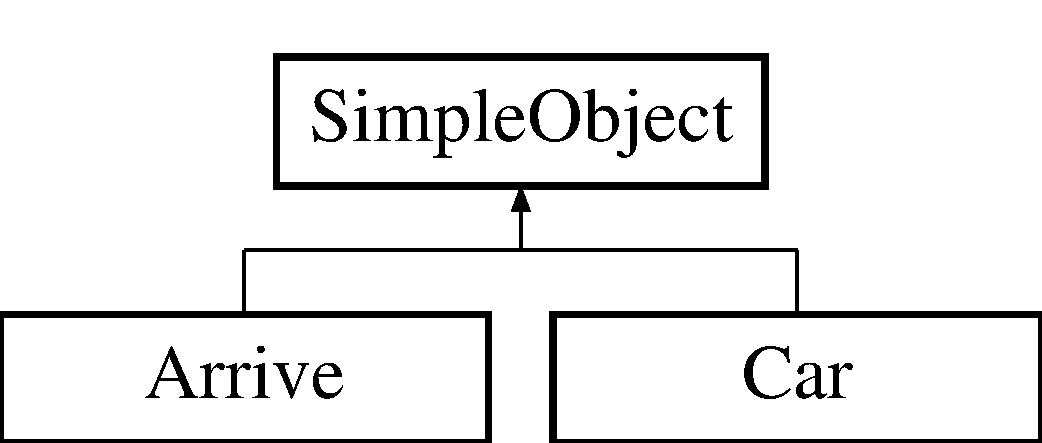
\includegraphics[height=2.000000cm]{classSimpleObject}
\end{center}
\end{figure}
\subsection*{Fonctions membres publiques}
\begin{DoxyCompactItemize}
\item 
virtual bool \hyperlink{classSimpleObject_ae9ea1f7ffe6d4aaf18f24e937e6b60ab}{set\-Position} (int8\-\_\-t x, int8\-\_\-t y)=0
\item 
virtual std\-::pair$<$ int8\-\_\-t, int8\-\_\-t $>$ \hyperlink{classSimpleObject_ae417f1a285ceab5a04130aba01bac856}{get\-Position} ()=0
\item 
virtual std\-::string \hyperlink{classSimpleObject_aedf0ddcc119ab40623b5b69badc9531a}{to\-String} ()=0
\end{DoxyCompactItemize}


\subsection{Documentation des fonctions membres}
\hypertarget{classSimpleObject_ae417f1a285ceab5a04130aba01bac856}{\index{Simple\-Object@{Simple\-Object}!get\-Position@{get\-Position}}
\index{get\-Position@{get\-Position}!SimpleObject@{Simple\-Object}}
\subsubsection[{get\-Position}]{\setlength{\rightskip}{0pt plus 5cm}virtual std\-::pair$<$int8\-\_\-t, int8\-\_\-t$>$ Simple\-Object\-::get\-Position (
\begin{DoxyParamCaption}
{}
\end{DoxyParamCaption}
)\hspace{0.3cm}{\ttfamily [pure virtual]}}}\label{classSimpleObject_ae417f1a285ceab5a04130aba01bac856}


Implémenté dans \hyperlink{classArrive_abe91e4a5bcf15ff987ab58c05b6bb537}{Arrive}, et \hyperlink{classCar_a20dd521474ee36b144bde58e3359eed6}{Car}.

\hypertarget{classSimpleObject_ae9ea1f7ffe6d4aaf18f24e937e6b60ab}{\index{Simple\-Object@{Simple\-Object}!set\-Position@{set\-Position}}
\index{set\-Position@{set\-Position}!SimpleObject@{Simple\-Object}}
\subsubsection[{set\-Position}]{\setlength{\rightskip}{0pt plus 5cm}virtual bool Simple\-Object\-::set\-Position (
\begin{DoxyParamCaption}
\item[{int8\-\_\-t}]{x, }
\item[{int8\-\_\-t}]{y}
\end{DoxyParamCaption}
)\hspace{0.3cm}{\ttfamily [pure virtual]}}}\label{classSimpleObject_ae9ea1f7ffe6d4aaf18f24e937e6b60ab}


Implémenté dans \hyperlink{classArrive_ab0484a9338e3774c5fa824153b1470e2}{Arrive}, et \hyperlink{classCar_a97e3c5de8eb65659ef520de6591f814d}{Car}.

\hypertarget{classSimpleObject_aedf0ddcc119ab40623b5b69badc9531a}{\index{Simple\-Object@{Simple\-Object}!to\-String@{to\-String}}
\index{to\-String@{to\-String}!SimpleObject@{Simple\-Object}}
\subsubsection[{to\-String}]{\setlength{\rightskip}{0pt plus 5cm}virtual std\-::string Simple\-Object\-::to\-String (
\begin{DoxyParamCaption}
{}
\end{DoxyParamCaption}
)\hspace{0.3cm}{\ttfamily [pure virtual]}}}\label{classSimpleObject_aedf0ddcc119ab40623b5b69badc9531a}


Implémenté dans \hyperlink{classArrive_af97f0e7e0624cce7ca09d52675e19872}{Arrive}, et \hyperlink{classCar_afb39c5a80ff1977ee13cb1e5cdf2fecd}{Car}.



La documentation de cette classe a été générée à partir du fichier suivant \-:\begin{DoxyCompactItemize}
\item 
headers/abstract/\hyperlink{simpleobject_8h}{simpleobject.\-h}\end{DoxyCompactItemize}

\hypertarget{classsServer}{\section{Référence de la classe s\-Server}
\label{classsServer}\index{s\-Server@{s\-Server}}
}


{\ttfamily \#include $<$share\-\_\-server.\-h$>$}

\subsection*{Fonctions membres publiques}
\begin{DoxyCompactItemize}
\item 
bool \hyperlink{classsServer_abcd4016d1b93c045f0847a48afee0ac2}{send\-Things\-To} (const char $\ast$, char $\ast$)
\item 
bool \hyperlink{classsServer_a62561438ad0563d99bf05e84795807f9}{is\-Connected} ()
\end{DoxyCompactItemize}
\subsection*{Fonctions membres publiques statiques}
\begin{DoxyCompactItemize}
\item 
static \hyperlink{classsServer}{s\-Server} $\ast$ \hyperlink{classsServer_af98a4a292c1beaab9296a88dba9f0c13}{get\-Instance} ()
\end{DoxyCompactItemize}
\subsection*{Fonctions membres privées}
\begin{DoxyCompactItemize}
\item 
\hyperlink{classsServer_ade1889963bc8ec1d6c184f900f1c4977}{s\-Server} ()
\item 
\hyperlink{classsServer_a1c9ed39e48d26a4ed531741979ced7bd}{$\sim$s\-Server} ()
\end{DoxyCompactItemize}
\subsection*{Attributs privés}
\begin{DoxyCompactItemize}
\item 
bool \hyperlink{classsServer_adeee5a2ac165a0d9df35757d2ddfc70d}{is\-\_\-connected}
\item 
key\-\_\-t \hyperlink{classsServer_a9300a483fb708e2e0208d5e1e53e0c97}{key\-\_\-send}
\item 
int \hyperlink{classsServer_ab7c99a899b82ac73c36c30da01ab7944}{shmid\-\_\-send}
\item 
\hyperlink{share__server_8h_ad73ea60fc164d7d224a2499bd77a1f35}{share\-Memory\-\_\-t} $\ast$ \hyperlink{classsServer_ad24c799f06a327db74a17fd30c78eff5}{data\-\_\-send}
\end{DoxyCompactItemize}
\subsection*{Attributs privés statiques}
\begin{DoxyCompactItemize}
\item 
static \hyperlink{classsServer}{s\-Server} $\ast$ \hyperlink{classsServer_a5567b4d6b98047dbc17c7c4072a71a62}{instance} = nullptr
\end{DoxyCompactItemize}


\subsection{Documentation des constructeurs et destructeur}
\hypertarget{classsServer_ade1889963bc8ec1d6c184f900f1c4977}{\index{s\-Server@{s\-Server}!s\-Server@{s\-Server}}
\index{s\-Server@{s\-Server}!sServer@{s\-Server}}
\subsubsection[{s\-Server}]{\setlength{\rightskip}{0pt plus 5cm}s\-Server\-::s\-Server (
\begin{DoxyParamCaption}
{}
\end{DoxyParamCaption}
)\hspace{0.3cm}{\ttfamily [private]}}}\label{classsServer_ade1889963bc8ec1d6c184f900f1c4977}


Références data\-\_\-send, I\-D\-\_\-\-C\-O\-N\-N\-E\-C\-T\-I\-O\-N, \-\_\-share\-M\-::index, I\-N\-T\-E\-R\-\_\-\-P\-R\-O\-C, key\-\_\-send, send\-Things\-To(), et shmid\-\_\-send.



Référencé par get\-Instance().


\begin{DoxyCode}
17                 \{
18     \hyperlink{classsServer_ad24c799f06a327db74a17fd30c78eff5}{data\_send} = (\hyperlink{server_8cpp_struct__shareM}{shareMemory\_t}*)std::malloc(\textcolor{keyword}{sizeof}(
      \hyperlink{server_8cpp_struct__shareM}{shareMemory\_t}));
19     \hyperlink{classsServer_ad24c799f06a327db74a17fd30c78eff5}{data\_send}->\hyperlink{server_8cpp_a30792c4b007e8273d3832fe2d5e70987}{index} = 0;
20 
21     \hyperlink{classsServer_a9300a483fb708e2e0208d5e1e53e0c97}{key\_send} = ftok(\textcolor{stringliteral}{"server.cpp"}, \textcolor{charliteral}{'R'});
22     \hyperlink{classsServer_ab7c99a899b82ac73c36c30da01ab7944}{shmid\_send} = shmget(\hyperlink{classsServer_a9300a483fb708e2e0208d5e1e53e0c97}{key\_send}, \textcolor{keyword}{sizeof}(\hyperlink{server_8cpp_struct__shareM}{shareMemory\_t}), 0644 | IPC\_CREAT);
23     \hyperlink{classsServer_ad24c799f06a327db74a17fd30c78eff5}{data\_send} = (\hyperlink{server_8cpp_struct__shareM}{shareMemory\_t}*)shmat(\hyperlink{classsServer_ab7c99a899b82ac73c36c30da01ab7944}{shmid\_send}, (\textcolor{keywordtype}{void}*)0, 0);
24 
25     \hyperlink{classsServer_abcd4016d1b93c045f0847a48afee0ac2}{sendThingsTo}(\hyperlink{definition_8h_abc8437510f986871fa5cdbcc7ca4bc31}{ID\_CONNECTION}, \hyperlink{definition_8h_a21b057a10e6f83a147922faf49652ac5}{INTER\_PROC});
26 \}
\end{DoxyCode}
\hypertarget{classsServer_a1c9ed39e48d26a4ed531741979ced7bd}{\index{s\-Server@{s\-Server}!$\sim$s\-Server@{$\sim$s\-Server}}
\index{$\sim$s\-Server@{$\sim$s\-Server}!sServer@{s\-Server}}
\subsubsection[{$\sim$s\-Server}]{\setlength{\rightskip}{0pt plus 5cm}s\-Server\-::$\sim$s\-Server (
\begin{DoxyParamCaption}
{}
\end{DoxyParamCaption}
)\hspace{0.3cm}{\ttfamily [inline]}, {\ttfamily [private]}}}\label{classsServer_a1c9ed39e48d26a4ed531741979ced7bd}


Références data\-\_\-send, et shmid\-\_\-send.


\begin{DoxyCode}
36                   \{
37             shmctl(\hyperlink{classsServer_ab7c99a899b82ac73c36c30da01ab7944}{shmid\_send}, IPC\_RMID, NULL);
38             \textcolor{keyword}{delete} \hyperlink{classsServer_ad24c799f06a327db74a17fd30c78eff5}{data\_send};
39         \}
\end{DoxyCode}


\subsection{Documentation des fonctions membres}
\hypertarget{classsServer_af98a4a292c1beaab9296a88dba9f0c13}{\index{s\-Server@{s\-Server}!get\-Instance@{get\-Instance}}
\index{get\-Instance@{get\-Instance}!sServer@{s\-Server}}
\subsubsection[{get\-Instance}]{\setlength{\rightskip}{0pt plus 5cm}{\bf s\-Server} $\ast$ s\-Server\-::get\-Instance (
\begin{DoxyParamCaption}
{}
\end{DoxyParamCaption}
)\hspace{0.3cm}{\ttfamily [static]}}}\label{classsServer_af98a4a292c1beaab9296a88dba9f0c13}


Références instance, et s\-Server().



Référencé par main().


\begin{DoxyCode}
10                              \{
11     \textcolor{keywordflow}{if}(\hyperlink{classsServer_a5567b4d6b98047dbc17c7c4072a71a62}{instance} == \textcolor{keyword}{nullptr})\{
12         \hyperlink{classsServer_a5567b4d6b98047dbc17c7c4072a71a62}{instance} = \textcolor{keyword}{new} \hyperlink{classsServer_ade1889963bc8ec1d6c184f900f1c4977}{sServer}();
13     \}
14     \textcolor{keywordflow}{return} \hyperlink{classsServer_a5567b4d6b98047dbc17c7c4072a71a62}{instance};
15 \}
\end{DoxyCode}
\hypertarget{classsServer_a62561438ad0563d99bf05e84795807f9}{\index{s\-Server@{s\-Server}!is\-Connected@{is\-Connected}}
\index{is\-Connected@{is\-Connected}!sServer@{s\-Server}}
\subsubsection[{is\-Connected}]{\setlength{\rightskip}{0pt plus 5cm}bool s\-Server\-::is\-Connected (
\begin{DoxyParamCaption}
{}
\end{DoxyParamCaption}
)\hspace{0.3cm}{\ttfamily [inline]}}}\label{classsServer_a62561438ad0563d99bf05e84795807f9}


Références is\-\_\-connected.


\begin{DoxyCode}
26                           \{
27             \textcolor{keywordflow}{return} \hyperlink{classsServer_adeee5a2ac165a0d9df35757d2ddfc70d}{is\_connected};
28         \}
\end{DoxyCode}
\hypertarget{classsServer_abcd4016d1b93c045f0847a48afee0ac2}{\index{s\-Server@{s\-Server}!send\-Things\-To@{send\-Things\-To}}
\index{send\-Things\-To@{send\-Things\-To}!sServer@{s\-Server}}
\subsubsection[{send\-Things\-To}]{\setlength{\rightskip}{0pt plus 5cm}bool s\-Server\-::send\-Things\-To (
\begin{DoxyParamCaption}
\item[{const char $\ast$}]{id\-\_\-code, }
\item[{char $\ast$}]{msg}
\end{DoxyParamCaption}
)}}\label{classsServer_abcd4016d1b93c045f0847a48afee0ac2}


Références data\-\_\-send, \-\_\-share\-M\-::id\-\_\-code, \-\_\-share\-M\-::index, et \-\_\-share\-M\-::tostring.



Référencé par main(), et s\-Server().


\begin{DoxyCode}
28                                                         \{
29     uint8\_t \hyperlink{server_8cpp_a30792c4b007e8273d3832fe2d5e70987}{index} = \hyperlink{classsServer_ad24c799f06a327db74a17fd30c78eff5}{data\_send}->\hyperlink{server_8cpp_a30792c4b007e8273d3832fe2d5e70987}{index};
30     strcpy(\hyperlink{classsServer_ad24c799f06a327db74a17fd30c78eff5}{data\_send}->\hyperlink{server_8cpp_ad57018c4c874c265b1dbfedba6c53e2c}{id\_code}, \hyperlink{server_8cpp_ad57018c4c874c265b1dbfedba6c53e2c}{id\_code});
31     strcpy(\hyperlink{classsServer_ad24c799f06a327db74a17fd30c78eff5}{data\_send}->\hyperlink{server_8cpp_a9b7627fd1c2693c3ecc662457fee4aba}{tostring}, msg);
32     \hyperlink{classsServer_ad24c799f06a327db74a17fd30c78eff5}{data\_send}->\hyperlink{server_8cpp_a30792c4b007e8273d3832fe2d5e70987}{index} = index + 1;
33 \}
\end{DoxyCode}


\subsection{Documentation des données membres}
\hypertarget{classsServer_ad24c799f06a327db74a17fd30c78eff5}{\index{s\-Server@{s\-Server}!data\-\_\-send@{data\-\_\-send}}
\index{data\-\_\-send@{data\-\_\-send}!sServer@{s\-Server}}
\subsubsection[{data\-\_\-send}]{\setlength{\rightskip}{0pt plus 5cm}{\bf share\-Memory\-\_\-t}$\ast$ s\-Server\-::data\-\_\-send\hspace{0.3cm}{\ttfamily [private]}}}\label{classsServer_ad24c799f06a327db74a17fd30c78eff5}


Référencé par send\-Things\-To(), s\-Server(), et $\sim$s\-Server().

\hypertarget{classsServer_a5567b4d6b98047dbc17c7c4072a71a62}{\index{s\-Server@{s\-Server}!instance@{instance}}
\index{instance@{instance}!sServer@{s\-Server}}
\subsubsection[{instance}]{\setlength{\rightskip}{0pt plus 5cm}{\bf s\-Server} $\ast$ s\-Server\-::instance = nullptr\hspace{0.3cm}{\ttfamily [static]}, {\ttfamily [private]}}}\label{classsServer_a5567b4d6b98047dbc17c7c4072a71a62}


Référencé par get\-Instance().

\hypertarget{classsServer_adeee5a2ac165a0d9df35757d2ddfc70d}{\index{s\-Server@{s\-Server}!is\-\_\-connected@{is\-\_\-connected}}
\index{is\-\_\-connected@{is\-\_\-connected}!sServer@{s\-Server}}
\subsubsection[{is\-\_\-connected}]{\setlength{\rightskip}{0pt plus 5cm}bool s\-Server\-::is\-\_\-connected\hspace{0.3cm}{\ttfamily [private]}}}\label{classsServer_adeee5a2ac165a0d9df35757d2ddfc70d}


Référencé par is\-Connected().

\hypertarget{classsServer_a9300a483fb708e2e0208d5e1e53e0c97}{\index{s\-Server@{s\-Server}!key\-\_\-send@{key\-\_\-send}}
\index{key\-\_\-send@{key\-\_\-send}!sServer@{s\-Server}}
\subsubsection[{key\-\_\-send}]{\setlength{\rightskip}{0pt plus 5cm}key\-\_\-t s\-Server\-::key\-\_\-send\hspace{0.3cm}{\ttfamily [private]}}}\label{classsServer_a9300a483fb708e2e0208d5e1e53e0c97}


Référencé par s\-Server().

\hypertarget{classsServer_ab7c99a899b82ac73c36c30da01ab7944}{\index{s\-Server@{s\-Server}!shmid\-\_\-send@{shmid\-\_\-send}}
\index{shmid\-\_\-send@{shmid\-\_\-send}!sServer@{s\-Server}}
\subsubsection[{shmid\-\_\-send}]{\setlength{\rightskip}{0pt plus 5cm}int s\-Server\-::shmid\-\_\-send\hspace{0.3cm}{\ttfamily [private]}}}\label{classsServer_ab7c99a899b82ac73c36c30da01ab7944}


Référencé par s\-Server(), et $\sim$s\-Server().



La documentation de cette classe a été générée à partir des fichiers suivants \-:\begin{DoxyCompactItemize}
\item 
headers/serveur/\hyperlink{share__server_8h}{share\-\_\-server.\-h}\item 
sources/server/\hyperlink{sserver_8cpp}{sserver.\-cpp}\end{DoxyCompactItemize}

\chapter{Documentation des fichiers}
\hypertarget{multipleobject_8h}{\section{headers/abstract/multipleobject.h File Reference}
\label{multipleobject_8h}\index{headers/abstract/multipleobject.\-h@{headers/abstract/multipleobject.\-h}}
}


add Position with X and Y  Virtual function  


{\ttfamily \#include $<$string$>$}\\*
Include dependency graph for multipleobject.\-h\-:
This graph shows which files directly or indirectly include this file\-:
\subsection*{Classes}
\begin{DoxyCompactItemize}
\item 
class \hyperlink{class_multiple_object}{Multiple\-Object}
\end{DoxyCompactItemize}


\subsection{Detailed Description}
add Position with X and Y  Virtual function return list of position  Virtual function

clear list of position  Virtual function

has Position  Virtual function

remove Position with X and Y  Virtual function

\begin{DoxyVersion}{Version}
1.\-0
\end{DoxyVersion}

\begin{DoxyParams}{Parameters}
{\em x} & position x 0 to 127 \\
\hline
{\em y} & position y 0 to 127 \\
\hline
\end{DoxyParams}
\begin{DoxyReturn}{Returns}
true true if succefully added 

false false if doesn't succefully added
\end{DoxyReturn}
\begin{DoxyVersion}{Version}
1.\-0
\end{DoxyVersion}

\begin{DoxyParams}{Parameters}
{\em x} & position x 0 to 127 \\
\hline
{\em y} & position y 0 to 127 \\
\hline
\end{DoxyParams}
\begin{DoxyReturn}{Returns}
true true if succefully removed 

false false if doesn't succefully removed
\end{DoxyReturn}
\begin{DoxyVersion}{Version}
1.\-0
\end{DoxyVersion}

\begin{DoxyParams}{Parameters}
{\em x} & position x 0 to 127 \\
\hline
{\em y} & position y 0 to 127 \\
\hline
\end{DoxyParams}
\begin{DoxyReturn}{Returns}
true has position set 

false has not position set
\end{DoxyReturn}
\begin{DoxyVersion}{Version}
1.\-0
\end{DoxyVersion}
\begin{DoxyReturn}{Returns}
true true if succefully clear 

false false if doesn't succefully clear
\end{DoxyReturn}
\begin{DoxyVersion}{Version}
1.\-0
\end{DoxyVersion}
\begin{DoxyReturn}{Returns}
std\-::string to\-String() function list to string 
\end{DoxyReturn}


Definition in file \hyperlink{multipleobject_8h_source}{multipleobject.\-h}.


\hypertarget{simpleobject_8h}{\section{headers/abstract/simpleobject.h File Reference}
\label{simpleobject_8h}\index{headers/abstract/simpleobject.\-h@{headers/abstract/simpleobject.\-h}}
}


set the position of object (car, arrival, start)  Virtual function  


{\ttfamily \#include $<$sstream$>$}\\*
{\ttfamily \#include $<$string$>$}\\*
{\ttfamily \#include $<$utility$>$}\\*
Include dependency graph for simpleobject.\-h\-:
This graph shows which files directly or indirectly include this file\-:
\subsection*{Classes}
\begin{DoxyCompactItemize}
\item 
class \hyperlink{class_simple_object}{Simple\-Object}
\end{DoxyCompactItemize}


\subsection{Detailed Description}
set the position of object (car, arrival, start)  Virtual function return the position to String  Virtual function

get the position of object (car, arrival, start)  Virtual function

\begin{DoxyVersion}{Version}
1.\-0
\end{DoxyVersion}

\begin{DoxyParams}{Parameters}
{\em x} & position x 0 to 127 \\
\hline
{\em y} & position y 0 to 127 \\
\hline
\end{DoxyParams}
\begin{DoxyReturn}{Returns}
true true if position correctly change 

false false if position not correctly change
\end{DoxyReturn}
\begin{DoxyVersion}{Version}
1.\-0
\end{DoxyVersion}
\begin{DoxyReturn}{Returns}
std\-::pair$<$int8\-\_\-t, int8\-\_\-t$>$ return the position of object
\end{DoxyReturn}
\begin{DoxyVersion}{Version}
1.\-0
\end{DoxyVersion}
\begin{DoxyReturn}{Returns}
std\-::string to\-String() function position to string 
\end{DoxyReturn}

\hypertarget{core_8h}{\section{Référence du fichier headers/core.h}
\label{core_8h}\index{headers/core.\-h@{headers/core.\-h}}
}
{\ttfamily \#include \char`\"{}../headers/manager.\-h\char`\"{}}\\*
{\ttfamily \#include \char`\"{}../headers/traitement/pathfinding.\-h\char`\"{}}\\*
{\ttfamily \#include \char`\"{}../headers/traitement/images.\-h\char`\"{}}\\*
\subsection*{Classes}
\begin{DoxyCompactItemize}
\item 
struct \hyperlink{core_8h_struct__stateMachine}{\-\_\-state\-Machine}
\item 
class \hyperlink{classCore}{Core}
\end{DoxyCompactItemize}
\subsection*{Énumérations}
\begin{DoxyCompactItemize}
\item 
enum \hyperlink{core_8h_a5d74787dedbc4e11c1ab15bf487e61f8}{State} \{ \hyperlink{core_8h_a5d74787dedbc4e11c1ab15bf487e61f8ab50339a10e1de285ac99d4c3990b8693}{State\-::\-N\-O\-N\-E} =0, 
\hyperlink{core_8h_a5d74787dedbc4e11c1ab15bf487e61f8ae0aa021e21dddbd6d8cecec71e9cf564}{State\-::\-O\-K}, 
\hyperlink{core_8h_a5d74787dedbc4e11c1ab15bf487e61f8ac2f3f489a00553e7a01d369c103c7251}{State\-::\-N\-O}, 
\hyperlink{core_8h_a5d74787dedbc4e11c1ab15bf487e61f8abb1ca97ec761fc37101737ba0aa2e7c5}{State\-::\-E\-R\-R\-O\-R}
 \}
\item 
enum \hyperlink{core_8h_a46c8a310cf4c094f8c80e1cb8dc1f911}{Mode} \{ \hyperlink{core_8h_a46c8a310cf4c094f8c80e1cb8dc1f911acf535b39ede8798cd6b56d99271afeef}{Mode\-::\-Stop\-\_\-\-Mode} =0, 
\hyperlink{core_8h_a46c8a310cf4c094f8c80e1cb8dc1f911a62a2c1fd120cdb7005bf42408c887d9d}{Mode\-::\-Auto\-\_\-\-Mode}, 
\hyperlink{core_8h_a46c8a310cf4c094f8c80e1cb8dc1f911a6879e8dabec58a1e3e670eaddfdc7bf7}{Mode\-::\-Virtual\-\_\-\-Mode}, 
\hyperlink{core_8h_a46c8a310cf4c094f8c80e1cb8dc1f911a493c3024fdbbce51ec6d8d8b0feacf13}{Mode\-::\-Manual\-\_\-\-Mode}
 \}
\end{DoxyCompactItemize}


\subsection{Documentation des classes}
\index{\-\_\-state\-Machine@{\-\_\-state\-Machine}}\label{struct__stateMachine}
\hypertarget{core_8h_struct__stateMachine}{}
\subsubsection{struct \-\_\-state\-Machine}
\begin{DoxyFields}{Membres de classe}
\hypertarget{core_8h_a157036ced733a021849ebcbc98c27200}{\hyperlink{core_8h_a5d74787dedbc4e11c1ab15bf487e61f8}{State}}\label{core_8h_a157036ced733a021849ebcbc98c27200}
&
\-\_\-state\-Calibration&
\\
\hline

\hypertarget{core_8h_adbc0e51d4bed9b6da5c44e921e37dc32}{\hyperlink{core_8h_a5d74787dedbc4e11c1ab15bf487e61f8}{State}}\label{core_8h_adbc0e51d4bed9b6da5c44e921e37dc32}
&
\-\_\-state\-Image\-Block&
\\
\hline

\hypertarget{core_8h_aa6cc70d0567b403fb9e993a681f48b85}{\hyperlink{core_8h_a5d74787dedbc4e11c1ab15bf487e61f8}{State}}\label{core_8h_aa6cc70d0567b403fb9e993a681f48b85}
&
\-\_\-state\-I\-P\-C&
\\
\hline

\hypertarget{core_8h_a79ce614ae01c3759d155c03026384ca7}{\hyperlink{core_8h_a5d74787dedbc4e11c1ab15bf487e61f8}{State}}\label{core_8h_a79ce614ae01c3759d155c03026384ca7}
&
\-\_\-state\-Pathfinding&
\\
\hline

\hypertarget{core_8h_aaee24e4ab99a6f1243a46645188de8d0}{\hyperlink{core_8h_a5d74787dedbc4e11c1ab15bf487e61f8}{State}}\label{core_8h_aaee24e4ab99a6f1243a46645188de8d0}
&
\-\_\-state\-Server&
\\
\hline

\hypertarget{core_8h_a88c6e0c15cdd29b3eec2e842fa09b08f}{\hyperlink{core_8h_a5d74787dedbc4e11c1ab15bf487e61f8}{State}}\label{core_8h_a88c6e0c15cdd29b3eec2e842fa09b08f}
&
\-\_\-state\-Trajectory&
\\
\hline

\end{DoxyFields}


\subsection{Documentation du type de l'énumération}
\hypertarget{core_8h_a46c8a310cf4c094f8c80e1cb8dc1f911}{\index{core.\-h@{core.\-h}!Mode@{Mode}}
\index{Mode@{Mode}!core.h@{core.\-h}}
\subsubsection[{Mode}]{\setlength{\rightskip}{0pt plus 5cm}enum {\bf Mode}\hspace{0.3cm}{\ttfamily [strong]}}}\label{core_8h_a46c8a310cf4c094f8c80e1cb8dc1f911}
\begin{Desc}
\item[Valeurs énumérées]\par
\begin{description}
\index{Stop\-\_\-\-Mode@{Stop\-\_\-\-Mode}!core.\-h@{core.\-h}}\index{core.\-h@{core.\-h}!Stop\-\_\-\-Mode@{Stop\-\_\-\-Mode}}\item[{\em 
\hypertarget{core_8h_a46c8a310cf4c094f8c80e1cb8dc1f911acf535b39ede8798cd6b56d99271afeef}{Stop\-\_\-\-Mode}\label{core_8h_a46c8a310cf4c094f8c80e1cb8dc1f911acf535b39ede8798cd6b56d99271afeef}
}]\index{Auto\-\_\-\-Mode@{Auto\-\_\-\-Mode}!core.\-h@{core.\-h}}\index{core.\-h@{core.\-h}!Auto\-\_\-\-Mode@{Auto\-\_\-\-Mode}}\item[{\em 
\hypertarget{core_8h_a46c8a310cf4c094f8c80e1cb8dc1f911a62a2c1fd120cdb7005bf42408c887d9d}{Auto\-\_\-\-Mode}\label{core_8h_a46c8a310cf4c094f8c80e1cb8dc1f911a62a2c1fd120cdb7005bf42408c887d9d}
}]\index{Virtual\-\_\-\-Mode@{Virtual\-\_\-\-Mode}!core.\-h@{core.\-h}}\index{core.\-h@{core.\-h}!Virtual\-\_\-\-Mode@{Virtual\-\_\-\-Mode}}\item[{\em 
\hypertarget{core_8h_a46c8a310cf4c094f8c80e1cb8dc1f911a6879e8dabec58a1e3e670eaddfdc7bf7}{Virtual\-\_\-\-Mode}\label{core_8h_a46c8a310cf4c094f8c80e1cb8dc1f911a6879e8dabec58a1e3e670eaddfdc7bf7}
}]\index{Manual\-\_\-\-Mode@{Manual\-\_\-\-Mode}!core.\-h@{core.\-h}}\index{core.\-h@{core.\-h}!Manual\-\_\-\-Mode@{Manual\-\_\-\-Mode}}\item[{\em 
\hypertarget{core_8h_a46c8a310cf4c094f8c80e1cb8dc1f911a493c3024fdbbce51ec6d8d8b0feacf13}{Manual\-\_\-\-Mode}\label{core_8h_a46c8a310cf4c094f8c80e1cb8dc1f911a493c3024fdbbce51ec6d8d8b0feacf13}
}]\end{description}
\end{Desc}

\begin{DoxyCode}
20 \{ \hyperlink{core_8h_a46c8a310cf4c094f8c80e1cb8dc1f911acf535b39ede8798cd6b56d99271afeef}{Stop\_Mode}=0, \hyperlink{core_8h_a46c8a310cf4c094f8c80e1cb8dc1f911a62a2c1fd120cdb7005bf42408c887d9d}{Auto\_Mode}, \hyperlink{core_8h_a46c8a310cf4c094f8c80e1cb8dc1f911a6879e8dabec58a1e3e670eaddfdc7bf7}{Virtual\_Mode}, 
      \hyperlink{core_8h_a46c8a310cf4c094f8c80e1cb8dc1f911a493c3024fdbbce51ec6d8d8b0feacf13}{Manual\_Mode} \};
\end{DoxyCode}
\hypertarget{core_8h_a5d74787dedbc4e11c1ab15bf487e61f8}{\index{core.\-h@{core.\-h}!State@{State}}
\index{State@{State}!core.h@{core.\-h}}
\subsubsection[{State}]{\setlength{\rightskip}{0pt plus 5cm}enum {\bf State}\hspace{0.3cm}{\ttfamily [strong]}}}\label{core_8h_a5d74787dedbc4e11c1ab15bf487e61f8}
\begin{Desc}
\item[Valeurs énumérées]\par
\begin{description}
\index{N\-O\-N\-E@{N\-O\-N\-E}!core.\-h@{core.\-h}}\index{core.\-h@{core.\-h}!N\-O\-N\-E@{N\-O\-N\-E}}\item[{\em 
\hypertarget{core_8h_a5d74787dedbc4e11c1ab15bf487e61f8ab50339a10e1de285ac99d4c3990b8693}{N\-O\-N\-E}\label{core_8h_a5d74787dedbc4e11c1ab15bf487e61f8ab50339a10e1de285ac99d4c3990b8693}
}]\index{O\-K@{O\-K}!core.\-h@{core.\-h}}\index{core.\-h@{core.\-h}!O\-K@{O\-K}}\item[{\em 
\hypertarget{core_8h_a5d74787dedbc4e11c1ab15bf487e61f8ae0aa021e21dddbd6d8cecec71e9cf564}{O\-K}\label{core_8h_a5d74787dedbc4e11c1ab15bf487e61f8ae0aa021e21dddbd6d8cecec71e9cf564}
}]\index{N\-O@{N\-O}!core.\-h@{core.\-h}}\index{core.\-h@{core.\-h}!N\-O@{N\-O}}\item[{\em 
\hypertarget{core_8h_a5d74787dedbc4e11c1ab15bf487e61f8ac2f3f489a00553e7a01d369c103c7251}{N\-O}\label{core_8h_a5d74787dedbc4e11c1ab15bf487e61f8ac2f3f489a00553e7a01d369c103c7251}
}]\index{E\-R\-R\-O\-R@{E\-R\-R\-O\-R}!core.\-h@{core.\-h}}\index{core.\-h@{core.\-h}!E\-R\-R\-O\-R@{E\-R\-R\-O\-R}}\item[{\em 
\hypertarget{core_8h_a5d74787dedbc4e11c1ab15bf487e61f8abb1ca97ec761fc37101737ba0aa2e7c5}{E\-R\-R\-O\-R}\label{core_8h_a5d74787dedbc4e11c1ab15bf487e61f8abb1ca97ec761fc37101737ba0aa2e7c5}
}]\end{description}
\end{Desc}

\begin{DoxyCode}
8 \{ \hyperlink{core_8h_a5d74787dedbc4e11c1ab15bf487e61f8ab50339a10e1de285ac99d4c3990b8693}{NONE}=0, \hyperlink{core_8h_a5d74787dedbc4e11c1ab15bf487e61f8ae0aa021e21dddbd6d8cecec71e9cf564}{OK}, \hyperlink{core_8h_a5d74787dedbc4e11c1ab15bf487e61f8ac2f3f489a00553e7a01d369c103c7251}{NO}, \hyperlink{core_8h_a5d74787dedbc4e11c1ab15bf487e61f8abb1ca97ec761fc37101737ba0aa2e7c5}{ERROR} \}; \textcolor{comment}{//NO is for pathfinding or trajectory if car can't move}
\end{DoxyCode}

\hypertarget{definition_8h}{\section{Référence du fichier headers/definition.h}
\label{definition_8h}\index{headers/definition.\-h@{headers/definition.\-h}}
}
\subsection*{Macros}
\begin{DoxyCompactItemize}
\item 
\#define \hyperlink{definition_8h_a3ec5cb9d22ac76105cb244c099e62bfa}{V\-I\-D\-E\-\_\-\-D\-E\-F}~0
\item 
\#define \hyperlink{definition_8h_a36aebf63f7666a150b14192119d9afa2}{C\-A\-R\-\_\-\-D\-E\-F}~3
\item 
\#define \hyperlink{definition_8h_a4d275339ef3ddec11c63b8b925b5b358}{B\-L\-O\-C\-\_\-\-D\-E\-F}~1
\item 
\#define \hyperlink{definition_8h_aff9c7c5f80f4fc67fbea9f7dce5cb5f7}{C\-H\-E\-M\-I\-N\-\_\-\-D\-E\-F}~4
\item 
\#define \hyperlink{definition_8h_a71cf532814b2e708da69ec435950685d}{A\-R\-R\-I\-V\-E\-\_\-\-D\-E\-F}~2
\item 
\#define \hyperlink{definition_8h_ad2cc26b8da12f6603455f84312aa649b}{C\-A\-M\-\_\-\-W\-I\-D\-T\-H}~640
\item 
\#define \hyperlink{definition_8h_ac88d2707293a4af9e155d57e3651162e}{C\-A\-M\-\_\-\-H\-E\-I\-G\-H\-T}~480
\item 
\#define \hyperlink{definition_8h_a9ddbbce2fd669544c295551b85ca01ff}{M\-A\-X\-\_\-\-B\-L\-O\-C\-\_\-\-S\-C\-E\-N\-E}~30
\item 
\#define \hyperlink{definition_8h_a7ff61b468299d760aa0a3187ab24dddc}{M\-A\-R\-G\-E\-\_\-\-B\-L\-O\-C\-K\-\_\-\-P\-R\-O\-C\-E\-S\-S\-I\-N\-G}~30
\item 
\#define \hyperlink{definition_8h_aa0e4cfe3919e1b2633bd67fbbae28ec5}{M\-A\-R\-K\-E\-R\-\_\-\-I\-D\-\_\-\-C\-A\-R}~1
\item 
\#define \hyperlink{definition_8h_a6b35f14504af015e91cc6963cb51d6f5}{M\-A\-R\-K\-E\-R\-\_\-\-I\-D\-\_\-\-A\-R\-R\-I\-V\-A\-L}~0
\item 
\#define \hyperlink{definition_8h_a6036f5d317ce1f843aae2fdd46d845c9}{M\-A\-R\-K\-E\-R\-\_\-\-I\-D\-\_\-\-A\-R\-E\-A}~12
\item 
\#define \hyperlink{definition_8h_a5c060ba02a1c2de42097ec04c0da0ea7}{M\-A\-X\-\_\-\-C\-O\-N\-N\-E\-C\-T\-I\-O\-N\-\_\-\-C\-L\-I\-E\-N\-T}~5
\item 
\#define \hyperlink{definition_8h_a752f5b785b69372034ac87e1a1598ce3}{P\-O\-R\-T\-\_\-\-S\-E\-R\-V\-E\-U\-R}~975
\item 
\#define \hyperlink{definition_8h_a0dec0c631f90a14aa6ff21617d54707a}{I\-D\-\_\-\-P\-C}~\char`\"{}b\-Fd6-\/a2e8-\/9\-Dff\textbackslash{}n\char`\"{}
\item 
\#define \hyperlink{definition_8h_aecf05b6e6a060d8da044532e9db74e2f}{I\-D\-\_\-\-C\-A\-R}~\char`\"{}59ef-\/6\-F70-\/4b\-M7\textbackslash{}n\char`\"{}
\item 
\#define \hyperlink{definition_8h_ad6b283a2d2326d0e040305c75ff08dc4}{I\-D\-\_\-\-R\-E\-M\-O\-T\-E}~\char`\"{}c3\-Z8-\/4b86-\/95\-Ax\textbackslash{}n\char`\"{}
\item 
\#define \hyperlink{definition_8h_abc8437510f986871fa5cdbcc7ca4bc31}{I\-D\-\_\-\-C\-O\-N\-N\-E\-C\-T\-I\-O\-N}~\char`\"{}xxxx-\/xxxx-\/xxxx\textbackslash{}n\char`\"{}
\item 
\#define \hyperlink{definition_8h_a21b057a10e6f83a147922faf49652ac5}{I\-N\-T\-E\-R\-\_\-\-P\-R\-O\-C}~\char`\"{}$<$P\-R\-O\-C\-\_\-\-E\-S\-T\-A\-B\-L\-I\-S\-H\-E\-D$>$\char`\"{}
\item 
\#define \hyperlink{definition_8h_adffc78b5b975243958cd1258f3cfb911}{R\-E\-Q\-\_\-\-C\-O\-D\-E}~\char`\"{}$<$I\-D-\/C\-O\-D\-E$>$\char`\"{}
\item 
\#define \hyperlink{definition_8h_a812f73a3ea946dbc24662a8736f64e55}{V\-A\-L\-\_\-\-C\-O\-D\-E}~\char`\"{}$<$I\-D-\/V\-A\-L\-I\-D$>$\char`\"{}
\item 
\#define \hyperlink{definition_8h_a6360244e5a8f026f28f31db5966308b4}{I\-N\-V\-A\-L\-\_\-\-C\-O\-D\-E}~\char`\"{}$<$I\-D-\/I\-N\-V\-A\-L\-I\-D$>$\char`\"{}
\item 
\#define \hyperlink{definition_8h_ab172dfb54371246ff3b8edc32639c033}{S\-T\-O\-P\-\_\-\-C\-O\-N\-N}~\char`\"{}$<$S\-T\-O\-P$>$\char`\"{}
\item 
\#define \hyperlink{definition_8h_a7f115ae3ca40562a74ac1330ce2e9581}{P\-A\-T\-H\-F\-I\-N\-D\-I\-N\-G}~0
\item 
\#define \hyperlink{definition_8h_a05e53db6bda5a9a3f102c6211668380a}{I\-M\-A\-G\-E\-S}~1
\item 
\#define \hyperlink{definition_8h_aeef0e3ba41fec73b731de55058a0e9a6}{S\-E\-R\-V\-E\-U\-R}~2
\end{DoxyCompactItemize}
\subsection*{Variables}
\begin{DoxyCompactItemize}
\item 
static bool \hyperlink{definition_8h_a117352cc494cc62c6b2f1882786a332c}{D\-E\-B\-U\-G} = true
\end{DoxyCompactItemize}


\subsection{Documentation des macros}
\hypertarget{definition_8h_a71cf532814b2e708da69ec435950685d}{\index{definition.\-h@{definition.\-h}!A\-R\-R\-I\-V\-E\-\_\-\-D\-E\-F@{A\-R\-R\-I\-V\-E\-\_\-\-D\-E\-F}}
\index{A\-R\-R\-I\-V\-E\-\_\-\-D\-E\-F@{A\-R\-R\-I\-V\-E\-\_\-\-D\-E\-F}!definition.h@{definition.\-h}}
\subsubsection[{A\-R\-R\-I\-V\-E\-\_\-\-D\-E\-F}]{\setlength{\rightskip}{0pt plus 5cm}\#define A\-R\-R\-I\-V\-E\-\_\-\-D\-E\-F~2}}\label{definition_8h_a71cf532814b2e708da69ec435950685d}


Référencé par Manager\-::update().

\hypertarget{definition_8h_a4d275339ef3ddec11c63b8b925b5b358}{\index{definition.\-h@{definition.\-h}!B\-L\-O\-C\-\_\-\-D\-E\-F@{B\-L\-O\-C\-\_\-\-D\-E\-F}}
\index{B\-L\-O\-C\-\_\-\-D\-E\-F@{B\-L\-O\-C\-\_\-\-D\-E\-F}!definition.h@{definition.\-h}}
\subsubsection[{B\-L\-O\-C\-\_\-\-D\-E\-F}]{\setlength{\rightskip}{0pt plus 5cm}\#define B\-L\-O\-C\-\_\-\-D\-E\-F~1}}\label{definition_8h_a4d275339ef3ddec11c63b8b925b5b358}


Référencé par Path\-Finding\-::\-Path\-Finding(), et Manager\-::update().

\hypertarget{definition_8h_ac88d2707293a4af9e155d57e3651162e}{\index{definition.\-h@{definition.\-h}!C\-A\-M\-\_\-\-H\-E\-I\-G\-H\-T@{C\-A\-M\-\_\-\-H\-E\-I\-G\-H\-T}}
\index{C\-A\-M\-\_\-\-H\-E\-I\-G\-H\-T@{C\-A\-M\-\_\-\-H\-E\-I\-G\-H\-T}!definition.h@{definition.\-h}}
\subsubsection[{C\-A\-M\-\_\-\-H\-E\-I\-G\-H\-T}]{\setlength{\rightskip}{0pt plus 5cm}\#define C\-A\-M\-\_\-\-H\-E\-I\-G\-H\-T~480}}\label{definition_8h_ac88d2707293a4af9e155d57e3651162e}
\hypertarget{definition_8h_ad2cc26b8da12f6603455f84312aa649b}{\index{definition.\-h@{definition.\-h}!C\-A\-M\-\_\-\-W\-I\-D\-T\-H@{C\-A\-M\-\_\-\-W\-I\-D\-T\-H}}
\index{C\-A\-M\-\_\-\-W\-I\-D\-T\-H@{C\-A\-M\-\_\-\-W\-I\-D\-T\-H}!definition.h@{definition.\-h}}
\subsubsection[{C\-A\-M\-\_\-\-W\-I\-D\-T\-H}]{\setlength{\rightskip}{0pt plus 5cm}\#define C\-A\-M\-\_\-\-W\-I\-D\-T\-H~640}}\label{definition_8h_ad2cc26b8da12f6603455f84312aa649b}
\hypertarget{definition_8h_a36aebf63f7666a150b14192119d9afa2}{\index{definition.\-h@{definition.\-h}!C\-A\-R\-\_\-\-D\-E\-F@{C\-A\-R\-\_\-\-D\-E\-F}}
\index{C\-A\-R\-\_\-\-D\-E\-F@{C\-A\-R\-\_\-\-D\-E\-F}!definition.h@{definition.\-h}}
\subsubsection[{C\-A\-R\-\_\-\-D\-E\-F}]{\setlength{\rightskip}{0pt plus 5cm}\#define C\-A\-R\-\_\-\-D\-E\-F~3}}\label{definition_8h_a36aebf63f7666a150b14192119d9afa2}


Référencé par Manager\-::update().

\hypertarget{definition_8h_aff9c7c5f80f4fc67fbea9f7dce5cb5f7}{\index{definition.\-h@{definition.\-h}!C\-H\-E\-M\-I\-N\-\_\-\-D\-E\-F@{C\-H\-E\-M\-I\-N\-\_\-\-D\-E\-F}}
\index{C\-H\-E\-M\-I\-N\-\_\-\-D\-E\-F@{C\-H\-E\-M\-I\-N\-\_\-\-D\-E\-F}!definition.h@{definition.\-h}}
\subsubsection[{C\-H\-E\-M\-I\-N\-\_\-\-D\-E\-F}]{\setlength{\rightskip}{0pt plus 5cm}\#define C\-H\-E\-M\-I\-N\-\_\-\-D\-E\-F~4}}\label{definition_8h_aff9c7c5f80f4fc67fbea9f7dce5cb5f7}


Référencé par Manager\-::update().

\hypertarget{definition_8h_aecf05b6e6a060d8da044532e9db74e2f}{\index{definition.\-h@{definition.\-h}!I\-D\-\_\-\-C\-A\-R@{I\-D\-\_\-\-C\-A\-R}}
\index{I\-D\-\_\-\-C\-A\-R@{I\-D\-\_\-\-C\-A\-R}!definition.h@{definition.\-h}}
\subsubsection[{I\-D\-\_\-\-C\-A\-R}]{\setlength{\rightskip}{0pt plus 5cm}\#define I\-D\-\_\-\-C\-A\-R~\char`\"{}59ef-\/6\-F70-\/4b\-M7\textbackslash{}n\char`\"{}}}\label{definition_8h_aecf05b6e6a060d8da044532e9db74e2f}


Référencé par Serveur\-::\-Accept\-And\-Dispatch(), main(), et Serveur\-::synchronize\-Client().

\hypertarget{definition_8h_abc8437510f986871fa5cdbcc7ca4bc31}{\index{definition.\-h@{definition.\-h}!I\-D\-\_\-\-C\-O\-N\-N\-E\-C\-T\-I\-O\-N@{I\-D\-\_\-\-C\-O\-N\-N\-E\-C\-T\-I\-O\-N}}
\index{I\-D\-\_\-\-C\-O\-N\-N\-E\-C\-T\-I\-O\-N@{I\-D\-\_\-\-C\-O\-N\-N\-E\-C\-T\-I\-O\-N}!definition.h@{definition.\-h}}
\subsubsection[{I\-D\-\_\-\-C\-O\-N\-N\-E\-C\-T\-I\-O\-N}]{\setlength{\rightskip}{0pt plus 5cm}\#define I\-D\-\_\-\-C\-O\-N\-N\-E\-C\-T\-I\-O\-N~\char`\"{}xxxx-\/xxxx-\/xxxx\textbackslash{}n\char`\"{}}}\label{definition_8h_abc8437510f986871fa5cdbcc7ca4bc31}


Référencé par main(), et s\-Server\-::s\-Server().

\hypertarget{definition_8h_a0dec0c631f90a14aa6ff21617d54707a}{\index{definition.\-h@{definition.\-h}!I\-D\-\_\-\-P\-C@{I\-D\-\_\-\-P\-C}}
\index{I\-D\-\_\-\-P\-C@{I\-D\-\_\-\-P\-C}!definition.h@{definition.\-h}}
\subsubsection[{I\-D\-\_\-\-P\-C}]{\setlength{\rightskip}{0pt plus 5cm}\#define I\-D\-\_\-\-P\-C~\char`\"{}b\-Fd6-\/a2e8-\/9\-Dff\textbackslash{}n\char`\"{}}}\label{definition_8h_a0dec0c631f90a14aa6ff21617d54707a}


Référencé par main(), et Serveur\-::synchronize\-Client().

\hypertarget{definition_8h_ad6b283a2d2326d0e040305c75ff08dc4}{\index{definition.\-h@{definition.\-h}!I\-D\-\_\-\-R\-E\-M\-O\-T\-E@{I\-D\-\_\-\-R\-E\-M\-O\-T\-E}}
\index{I\-D\-\_\-\-R\-E\-M\-O\-T\-E@{I\-D\-\_\-\-R\-E\-M\-O\-T\-E}!definition.h@{definition.\-h}}
\subsubsection[{I\-D\-\_\-\-R\-E\-M\-O\-T\-E}]{\setlength{\rightskip}{0pt plus 5cm}\#define I\-D\-\_\-\-R\-E\-M\-O\-T\-E~\char`\"{}c3\-Z8-\/4b86-\/95\-Ax\textbackslash{}n\char`\"{}}}\label{definition_8h_ad6b283a2d2326d0e040305c75ff08dc4}


Référencé par main(), et Serveur\-::synchronize\-Client().

\hypertarget{definition_8h_a05e53db6bda5a9a3f102c6211668380a}{\index{definition.\-h@{definition.\-h}!I\-M\-A\-G\-E\-S@{I\-M\-A\-G\-E\-S}}
\index{I\-M\-A\-G\-E\-S@{I\-M\-A\-G\-E\-S}!definition.h@{definition.\-h}}
\subsubsection[{I\-M\-A\-G\-E\-S}]{\setlength{\rightskip}{0pt plus 5cm}\#define I\-M\-A\-G\-E\-S~1}}\label{definition_8h_a05e53db6bda5a9a3f102c6211668380a}
\hypertarget{definition_8h_a21b057a10e6f83a147922faf49652ac5}{\index{definition.\-h@{definition.\-h}!I\-N\-T\-E\-R\-\_\-\-P\-R\-O\-C@{I\-N\-T\-E\-R\-\_\-\-P\-R\-O\-C}}
\index{I\-N\-T\-E\-R\-\_\-\-P\-R\-O\-C@{I\-N\-T\-E\-R\-\_\-\-P\-R\-O\-C}!definition.h@{definition.\-h}}
\subsubsection[{I\-N\-T\-E\-R\-\_\-\-P\-R\-O\-C}]{\setlength{\rightskip}{0pt plus 5cm}\#define I\-N\-T\-E\-R\-\_\-\-P\-R\-O\-C~\char`\"{}$<$P\-R\-O\-C\-\_\-\-E\-S\-T\-A\-B\-L\-I\-S\-H\-E\-D$>$\char`\"{}}}\label{definition_8h_a21b057a10e6f83a147922faf49652ac5}


Référencé par s\-Server\-::s\-Server().

\hypertarget{definition_8h_a6360244e5a8f026f28f31db5966308b4}{\index{definition.\-h@{definition.\-h}!I\-N\-V\-A\-L\-\_\-\-C\-O\-D\-E@{I\-N\-V\-A\-L\-\_\-\-C\-O\-D\-E}}
\index{I\-N\-V\-A\-L\-\_\-\-C\-O\-D\-E@{I\-N\-V\-A\-L\-\_\-\-C\-O\-D\-E}!definition.h@{definition.\-h}}
\subsubsection[{I\-N\-V\-A\-L\-\_\-\-C\-O\-D\-E}]{\setlength{\rightskip}{0pt plus 5cm}\#define I\-N\-V\-A\-L\-\_\-\-C\-O\-D\-E~\char`\"{}$<$I\-D-\/I\-N\-V\-A\-L\-I\-D$>$\char`\"{}}}\label{definition_8h_a6360244e5a8f026f28f31db5966308b4}


Référencé par Serveur\-::\-Accept\-And\-Dispatch().

\hypertarget{definition_8h_a7ff61b468299d760aa0a3187ab24dddc}{\index{definition.\-h@{definition.\-h}!M\-A\-R\-G\-E\-\_\-\-B\-L\-O\-C\-K\-\_\-\-P\-R\-O\-C\-E\-S\-S\-I\-N\-G@{M\-A\-R\-G\-E\-\_\-\-B\-L\-O\-C\-K\-\_\-\-P\-R\-O\-C\-E\-S\-S\-I\-N\-G}}
\index{M\-A\-R\-G\-E\-\_\-\-B\-L\-O\-C\-K\-\_\-\-P\-R\-O\-C\-E\-S\-S\-I\-N\-G@{M\-A\-R\-G\-E\-\_\-\-B\-L\-O\-C\-K\-\_\-\-P\-R\-O\-C\-E\-S\-S\-I\-N\-G}!definition.h@{definition.\-h}}
\subsubsection[{M\-A\-R\-G\-E\-\_\-\-B\-L\-O\-C\-K\-\_\-\-P\-R\-O\-C\-E\-S\-S\-I\-N\-G}]{\setlength{\rightskip}{0pt plus 5cm}\#define M\-A\-R\-G\-E\-\_\-\-B\-L\-O\-C\-K\-\_\-\-P\-R\-O\-C\-E\-S\-S\-I\-N\-G~30}}\label{definition_8h_a7ff61b468299d760aa0a3187ab24dddc}


Référencé par Images\-P\-::markers\-Processing().

\hypertarget{definition_8h_a6036f5d317ce1f843aae2fdd46d845c9}{\index{definition.\-h@{definition.\-h}!M\-A\-R\-K\-E\-R\-\_\-\-I\-D\-\_\-\-A\-R\-E\-A@{M\-A\-R\-K\-E\-R\-\_\-\-I\-D\-\_\-\-A\-R\-E\-A}}
\index{M\-A\-R\-K\-E\-R\-\_\-\-I\-D\-\_\-\-A\-R\-E\-A@{M\-A\-R\-K\-E\-R\-\_\-\-I\-D\-\_\-\-A\-R\-E\-A}!definition.h@{definition.\-h}}
\subsubsection[{M\-A\-R\-K\-E\-R\-\_\-\-I\-D\-\_\-\-A\-R\-E\-A}]{\setlength{\rightskip}{0pt plus 5cm}\#define M\-A\-R\-K\-E\-R\-\_\-\-I\-D\-\_\-\-A\-R\-E\-A~12}}\label{definition_8h_a6036f5d317ce1f843aae2fdd46d845c9}


Référencé par Images\-P\-::calibration(), et Images\-P\-::markers\-Processing().

\hypertarget{definition_8h_a6b35f14504af015e91cc6963cb51d6f5}{\index{definition.\-h@{definition.\-h}!M\-A\-R\-K\-E\-R\-\_\-\-I\-D\-\_\-\-A\-R\-R\-I\-V\-A\-L@{M\-A\-R\-K\-E\-R\-\_\-\-I\-D\-\_\-\-A\-R\-R\-I\-V\-A\-L}}
\index{M\-A\-R\-K\-E\-R\-\_\-\-I\-D\-\_\-\-A\-R\-R\-I\-V\-A\-L@{M\-A\-R\-K\-E\-R\-\_\-\-I\-D\-\_\-\-A\-R\-R\-I\-V\-A\-L}!definition.h@{definition.\-h}}
\subsubsection[{M\-A\-R\-K\-E\-R\-\_\-\-I\-D\-\_\-\-A\-R\-R\-I\-V\-A\-L}]{\setlength{\rightskip}{0pt plus 5cm}\#define M\-A\-R\-K\-E\-R\-\_\-\-I\-D\-\_\-\-A\-R\-R\-I\-V\-A\-L~0}}\label{definition_8h_a6b35f14504af015e91cc6963cb51d6f5}


Référencé par Images\-P\-::markers\-Processing().

\hypertarget{definition_8h_aa0e4cfe3919e1b2633bd67fbbae28ec5}{\index{definition.\-h@{definition.\-h}!M\-A\-R\-K\-E\-R\-\_\-\-I\-D\-\_\-\-C\-A\-R@{M\-A\-R\-K\-E\-R\-\_\-\-I\-D\-\_\-\-C\-A\-R}}
\index{M\-A\-R\-K\-E\-R\-\_\-\-I\-D\-\_\-\-C\-A\-R@{M\-A\-R\-K\-E\-R\-\_\-\-I\-D\-\_\-\-C\-A\-R}!definition.h@{definition.\-h}}
\subsubsection[{M\-A\-R\-K\-E\-R\-\_\-\-I\-D\-\_\-\-C\-A\-R}]{\setlength{\rightskip}{0pt plus 5cm}\#define M\-A\-R\-K\-E\-R\-\_\-\-I\-D\-\_\-\-C\-A\-R~1}}\label{definition_8h_aa0e4cfe3919e1b2633bd67fbbae28ec5}


Référencé par Images\-P\-::markers\-Processing(), et Images\-P\-::tracking\-Car().

\hypertarget{definition_8h_a9ddbbce2fd669544c295551b85ca01ff}{\index{definition.\-h@{definition.\-h}!M\-A\-X\-\_\-\-B\-L\-O\-C\-\_\-\-S\-C\-E\-N\-E@{M\-A\-X\-\_\-\-B\-L\-O\-C\-\_\-\-S\-C\-E\-N\-E}}
\index{M\-A\-X\-\_\-\-B\-L\-O\-C\-\_\-\-S\-C\-E\-N\-E@{M\-A\-X\-\_\-\-B\-L\-O\-C\-\_\-\-S\-C\-E\-N\-E}!definition.h@{definition.\-h}}
\subsubsection[{M\-A\-X\-\_\-\-B\-L\-O\-C\-\_\-\-S\-C\-E\-N\-E}]{\setlength{\rightskip}{0pt plus 5cm}\#define M\-A\-X\-\_\-\-B\-L\-O\-C\-\_\-\-S\-C\-E\-N\-E~30}}\label{definition_8h_a9ddbbce2fd669544c295551b85ca01ff}


Référencé par Bloc\-::\-Bloc().

\hypertarget{definition_8h_a5c060ba02a1c2de42097ec04c0da0ea7}{\index{definition.\-h@{definition.\-h}!M\-A\-X\-\_\-\-C\-O\-N\-N\-E\-C\-T\-I\-O\-N\-\_\-\-C\-L\-I\-E\-N\-T@{M\-A\-X\-\_\-\-C\-O\-N\-N\-E\-C\-T\-I\-O\-N\-\_\-\-C\-L\-I\-E\-N\-T}}
\index{M\-A\-X\-\_\-\-C\-O\-N\-N\-E\-C\-T\-I\-O\-N\-\_\-\-C\-L\-I\-E\-N\-T@{M\-A\-X\-\_\-\-C\-O\-N\-N\-E\-C\-T\-I\-O\-N\-\_\-\-C\-L\-I\-E\-N\-T}!definition.h@{definition.\-h}}
\subsubsection[{M\-A\-X\-\_\-\-C\-O\-N\-N\-E\-C\-T\-I\-O\-N\-\_\-\-C\-L\-I\-E\-N\-T}]{\setlength{\rightskip}{0pt plus 5cm}\#define M\-A\-X\-\_\-\-C\-O\-N\-N\-E\-C\-T\-I\-O\-N\-\_\-\-C\-L\-I\-E\-N\-T~5}}\label{definition_8h_a5c060ba02a1c2de42097ec04c0da0ea7}


Référencé par Serveur\-::\-Accept\-And\-Dispatch(), et Serveur\-::\-Serveur().

\hypertarget{definition_8h_a7f115ae3ca40562a74ac1330ce2e9581}{\index{definition.\-h@{definition.\-h}!P\-A\-T\-H\-F\-I\-N\-D\-I\-N\-G@{P\-A\-T\-H\-F\-I\-N\-D\-I\-N\-G}}
\index{P\-A\-T\-H\-F\-I\-N\-D\-I\-N\-G@{P\-A\-T\-H\-F\-I\-N\-D\-I\-N\-G}!definition.h@{definition.\-h}}
\subsubsection[{P\-A\-T\-H\-F\-I\-N\-D\-I\-N\-G}]{\setlength{\rightskip}{0pt plus 5cm}\#define P\-A\-T\-H\-F\-I\-N\-D\-I\-N\-G~0}}\label{definition_8h_a7f115ae3ca40562a74ac1330ce2e9581}
\hypertarget{definition_8h_a752f5b785b69372034ac87e1a1598ce3}{\index{definition.\-h@{definition.\-h}!P\-O\-R\-T\-\_\-\-S\-E\-R\-V\-E\-U\-R@{P\-O\-R\-T\-\_\-\-S\-E\-R\-V\-E\-U\-R}}
\index{P\-O\-R\-T\-\_\-\-S\-E\-R\-V\-E\-U\-R@{P\-O\-R\-T\-\_\-\-S\-E\-R\-V\-E\-U\-R}!definition.h@{definition.\-h}}
\subsubsection[{P\-O\-R\-T\-\_\-\-S\-E\-R\-V\-E\-U\-R}]{\setlength{\rightskip}{0pt plus 5cm}\#define P\-O\-R\-T\-\_\-\-S\-E\-R\-V\-E\-U\-R~975}}\label{definition_8h_a752f5b785b69372034ac87e1a1598ce3}


Référencé par Serveur\-::\-Serveur().

\hypertarget{definition_8h_adffc78b5b975243958cd1258f3cfb911}{\index{definition.\-h@{definition.\-h}!R\-E\-Q\-\_\-\-C\-O\-D\-E@{R\-E\-Q\-\_\-\-C\-O\-D\-E}}
\index{R\-E\-Q\-\_\-\-C\-O\-D\-E@{R\-E\-Q\-\_\-\-C\-O\-D\-E}!definition.h@{definition.\-h}}
\subsubsection[{R\-E\-Q\-\_\-\-C\-O\-D\-E}]{\setlength{\rightskip}{0pt plus 5cm}\#define R\-E\-Q\-\_\-\-C\-O\-D\-E~\char`\"{}$<$I\-D-\/C\-O\-D\-E$>$\char`\"{}}}\label{definition_8h_adffc78b5b975243958cd1258f3cfb911}


Référencé par Serveur\-::synchronize\-Client().

\hypertarget{definition_8h_aeef0e3ba41fec73b731de55058a0e9a6}{\index{definition.\-h@{definition.\-h}!S\-E\-R\-V\-E\-U\-R@{S\-E\-R\-V\-E\-U\-R}}
\index{S\-E\-R\-V\-E\-U\-R@{S\-E\-R\-V\-E\-U\-R}!definition.h@{definition.\-h}}
\subsubsection[{S\-E\-R\-V\-E\-U\-R}]{\setlength{\rightskip}{0pt plus 5cm}\#define S\-E\-R\-V\-E\-U\-R~2}}\label{definition_8h_aeef0e3ba41fec73b731de55058a0e9a6}
\hypertarget{definition_8h_ab172dfb54371246ff3b8edc32639c033}{\index{definition.\-h@{definition.\-h}!S\-T\-O\-P\-\_\-\-C\-O\-N\-N@{S\-T\-O\-P\-\_\-\-C\-O\-N\-N}}
\index{S\-T\-O\-P\-\_\-\-C\-O\-N\-N@{S\-T\-O\-P\-\_\-\-C\-O\-N\-N}!definition.h@{definition.\-h}}
\subsubsection[{S\-T\-O\-P\-\_\-\-C\-O\-N\-N}]{\setlength{\rightskip}{0pt plus 5cm}\#define S\-T\-O\-P\-\_\-\-C\-O\-N\-N~\char`\"{}$<$S\-T\-O\-P$>$\char`\"{}}}\label{definition_8h_ab172dfb54371246ff3b8edc32639c033}


Référencé par Serveur\-::\-Accept\-And\-Dispatch().

\hypertarget{definition_8h_a812f73a3ea946dbc24662a8736f64e55}{\index{definition.\-h@{definition.\-h}!V\-A\-L\-\_\-\-C\-O\-D\-E@{V\-A\-L\-\_\-\-C\-O\-D\-E}}
\index{V\-A\-L\-\_\-\-C\-O\-D\-E@{V\-A\-L\-\_\-\-C\-O\-D\-E}!definition.h@{definition.\-h}}
\subsubsection[{V\-A\-L\-\_\-\-C\-O\-D\-E}]{\setlength{\rightskip}{0pt plus 5cm}\#define V\-A\-L\-\_\-\-C\-O\-D\-E~\char`\"{}$<$I\-D-\/V\-A\-L\-I\-D$>$\char`\"{}}}\label{definition_8h_a812f73a3ea946dbc24662a8736f64e55}


Référencé par Serveur\-::\-Accept\-And\-Dispatch().

\hypertarget{definition_8h_a3ec5cb9d22ac76105cb244c099e62bfa}{\index{definition.\-h@{definition.\-h}!V\-I\-D\-E\-\_\-\-D\-E\-F@{V\-I\-D\-E\-\_\-\-D\-E\-F}}
\index{V\-I\-D\-E\-\_\-\-D\-E\-F@{V\-I\-D\-E\-\_\-\-D\-E\-F}!definition.h@{definition.\-h}}
\subsubsection[{V\-I\-D\-E\-\_\-\-D\-E\-F}]{\setlength{\rightskip}{0pt plus 5cm}\#define V\-I\-D\-E\-\_\-\-D\-E\-F~0}}\label{definition_8h_a3ec5cb9d22ac76105cb244c099e62bfa}


\subsection{Documentation des variables}
\hypertarget{definition_8h_a117352cc494cc62c6b2f1882786a332c}{\index{definition.\-h@{definition.\-h}!D\-E\-B\-U\-G@{D\-E\-B\-U\-G}}
\index{D\-E\-B\-U\-G@{D\-E\-B\-U\-G}!definition.h@{definition.\-h}}
\subsubsection[{D\-E\-B\-U\-G}]{\setlength{\rightskip}{0pt plus 5cm}bool D\-E\-B\-U\-G = true\hspace{0.3cm}{\ttfamily [static]}}}\label{definition_8h_a117352cc494cc62c6b2f1882786a332c}


Référencé par Core\-::auto\-Virtual\-Mode(), Core\-::block\-Processing(), et Core\-::start().


\hypertarget{manager_8h}{\section{Référence du fichier headers/manager.h}
\label{manager_8h}\index{headers/manager.\-h@{headers/manager.\-h}}
}


allow to know $\ast$\-\_\-\-D\-E\-F into the matrix (include \char`\"{}definition.\-h\char`\"{})  


{\ttfamily \#include \char`\"{}manager/car.\-h\char`\"{}}\\*
{\ttfamily \#include \char`\"{}manager/bloc.\-h\char`\"{}}\\*
{\ttfamily \#include \char`\"{}manager/chemin.\-h\char`\"{}}\\*
{\ttfamily \#include \char`\"{}manager/arrive.\-h\char`\"{}}\\*
{\ttfamily \#include $<$string$>$}\\*
{\ttfamily \#include $<$utility$>$}\\*
{\ttfamily \#include $<$stdlib.\-h$>$}\\*
{\ttfamily \#include $<$iostream$>$}\\*
\subsection*{Classes}
\begin{DoxyCompactItemize}
\item 
class \hyperlink{classManager}{Manager}
\end{DoxyCompactItemize}


\subsection{Description détaillée}
allow to know $\ast$\-\_\-\-D\-E\-F into the matrix (include \char`\"{}definition.\-h\char`\"{}) Singleton \hyperlink{classManager}{Manager()}

Destructor of the class.

Display the matrix into terminal.

Display info send to remote control (A\-P\-P\-L\-I)

create the Matrix

have the size of scene

have the Matrix

update add all block, car, arrive, path into matrix

\begin{DoxyVersion}{Version}
1.\-0
\end{DoxyVersion}

\begin{DoxyParams}{Paramètres}
{\em x} & position X 0 to 127 \\
\hline
{\em y} & position Y 0 to 127 \\
\hline
\end{DoxyParams}
\begin{DoxyReturn}{Renvoie}
int8\-\_\-t return (B\-L\-O\-C\-\_\-\-D\-E\-F, V\-I\-D\-E\-\_\-\-D\-E\-F, C\-A\-R\-\_\-\-D\-E\-F, A\-R\-R\-I\-V\-E\-\_\-\-D\-E\-F, ...)
\end{DoxyReturn}
\begin{DoxyVersion}{Version}
1.\-0

1.\-0
\end{DoxyVersion}
\begin{DoxyReturn}{Renvoie}
int8\-\_\-t$\ast$$\ast$ return the matrix max size 127x127
\end{DoxyReturn}
\begin{DoxyVersion}{Version}
1.\-0
\end{DoxyVersion}
\begin{DoxyReturn}{Renvoie}
int8\-\_\-t return size 0 to 127
\end{DoxyReturn}
\begin{DoxyVersion}{Version}
1.\-0
\end{DoxyVersion}
\begin{DoxyReturn}{Renvoie}
true matrix correctly created 

false matrix not correctly created
\end{DoxyReturn}
\begin{DoxyVersion}{Version}
1.\-0
\end{DoxyVersion}
\begin{DoxyReturn}{Renvoie}
std\-::string String to send in remote control 
\end{DoxyReturn}

\hypertarget{arrive_8h}{\section{Référence du fichier headers/manager/arrive.h}
\label{arrive_8h}\index{headers/manager/arrive.\-h@{headers/manager/arrive.\-h}}
}


Abstract of \hyperlink{classSimpleObject}{Simple\-Object}  Virtual function.  


{\ttfamily \#include $<$utility$>$}\\*
{\ttfamily \#include $<$string$>$}\\*
{\ttfamily \#include \char`\"{}../abstract/simpleobject.\-h\char`\"{}}\\*
\subsection*{Classes}
\begin{DoxyCompactItemize}
\item 
class \hyperlink{classArrive}{Arrive}
\end{DoxyCompactItemize}


\subsection{Description détaillée}
Abstract of \hyperlink{classSimpleObject}{Simple\-Object}  Virtual function. Abstract of \hyperlink{classMultipleObject}{Multiple\-Object}  Virtual function.

\begin{DoxyVersion}{Version}
1.\-0 
\end{DoxyVersion}

\hypertarget{bloc_8h}{\section{Référence du fichier headers/manager/bloc.h}
\label{bloc_8h}\index{headers/manager/bloc.\-h@{headers/manager/bloc.\-h}}
}


Abstract of \hyperlink{classMultipleObject}{Multiple\-Object}  Virtual function.  


{\ttfamily \#include $<$utility$>$}\\*
{\ttfamily \#include $<$vector$>$}\\*
{\ttfamily \#include $<$string$>$}\\*
{\ttfamily \#include \char`\"{}../abstract/multipleobject.\-h\char`\"{}}\\*
{\ttfamily \#include \char`\"{}../definition.\-h\char`\"{}}\\*
\subsection*{Classes}
\begin{DoxyCompactItemize}
\item 
class \hyperlink{classBloc}{Bloc}
\end{DoxyCompactItemize}


\subsection{Description détaillée}
Abstract of \hyperlink{classMultipleObject}{Multiple\-Object}  Virtual function. \begin{DoxyVersion}{Version}
1.\-0 
\end{DoxyVersion}

\hypertarget{car_8h}{\section{Référence du fichier headers/manager/car.h}
\label{car_8h}\index{headers/manager/car.\-h@{headers/manager/car.\-h}}
}


Abstract of \hyperlink{classSimpleObject}{Simple\-Object}  Virtual function.  


{\ttfamily \#include $<$utility$>$}\\*
{\ttfamily \#include $<$string$>$}\\*
{\ttfamily \#include \char`\"{}../abstract/simpleobject.\-h\char`\"{}}\\*
\subsection*{Classes}
\begin{DoxyCompactItemize}
\item 
class \hyperlink{classCar}{Car}
\end{DoxyCompactItemize}


\subsection{Description détaillée}
Abstract of \hyperlink{classSimpleObject}{Simple\-Object}  Virtual function. \begin{DoxyVersion}{Version}
1.\-0 
\end{DoxyVersion}

\hypertarget{chemin_8h}{\section{Référence du fichier headers/manager/chemin.h}
\label{chemin_8h}\index{headers/manager/chemin.\-h@{headers/manager/chemin.\-h}}
}
{\ttfamily \#include $<$utility$>$}\\*
{\ttfamily \#include $<$vector$>$}\\*
{\ttfamily \#include $<$string$>$}\\*
{\ttfamily \#include \char`\"{}../abstract/multipleobject.\-h\char`\"{}}\\*
\subsection*{Classes}
\begin{DoxyCompactItemize}
\item 
class \hyperlink{classChemin}{Chemin}
\end{DoxyCompactItemize}

\hypertarget{serveur_8h}{\section{Référence du fichier headers/manager/serveur.h}
\label{serveur_8h}\index{headers/manager/serveur.\-h@{headers/manager/serveur.\-h}}
}
{\ttfamily \#include \char`\"{}../definition.\-h\char`\"{}}\\*
{\ttfamily \#include $<$iostream$>$}\\*
{\ttfamily \#include $<$vector$>$}\\*
{\ttfamily \#include $<$cstdio$>$}\\*
{\ttfamily \#include $<$cstdlib$>$}\\*
{\ttfamily \#include $<$cstring$>$}\\*
{\ttfamily \#include $<$unistd.\-h$>$}\\*
{\ttfamily \#include $<$sys/socket.\-h$>$}\\*
{\ttfamily \#include $<$netinet/in.\-h$>$}\\*
{\ttfamily \#include \char`\"{}../serveur/client.\-h\char`\"{}}\\*
\subsection*{Classes}
\begin{DoxyCompactItemize}
\item 
class \hyperlink{classServeur}{Serveur}
\end{DoxyCompactItemize}

\hypertarget{client_8h}{\section{Référence du fichier headers/serveur/client.h}
\label{client_8h}\index{headers/serveur/client.\-h@{headers/serveur/client.\-h}}
}
{\ttfamily \#include $<$iostream$>$}\\*
{\ttfamily \#include $<$string$>$}\\*
{\ttfamily \#include $<$cstdio$>$}\\*
{\ttfamily \#include $<$cstdlib$>$}\\*
\subsection*{Classes}
\begin{DoxyCompactItemize}
\item 
class \hyperlink{classClient}{Client}
\end{DoxyCompactItemize}
\subsection*{Macros}
\begin{DoxyCompactItemize}
\item 
\#define \hyperlink{client_8h_adb8b7f0305183ffdba80cf2390ea33fa}{M\-A\-X\-\_\-\-N\-A\-M\-E\-\_\-\-L\-E\-N\-G\-H\-T}~20
\end{DoxyCompactItemize}


\subsection{Documentation des macros}
\hypertarget{client_8h_adb8b7f0305183ffdba80cf2390ea33fa}{\index{client.\-h@{client.\-h}!M\-A\-X\-\_\-\-N\-A\-M\-E\-\_\-\-L\-E\-N\-G\-H\-T@{M\-A\-X\-\_\-\-N\-A\-M\-E\-\_\-\-L\-E\-N\-G\-H\-T}}
\index{M\-A\-X\-\_\-\-N\-A\-M\-E\-\_\-\-L\-E\-N\-G\-H\-T@{M\-A\-X\-\_\-\-N\-A\-M\-E\-\_\-\-L\-E\-N\-G\-H\-T}!client.h@{client.\-h}}
\subsubsection[{M\-A\-X\-\_\-\-N\-A\-M\-E\-\_\-\-L\-E\-N\-G\-H\-T}]{\setlength{\rightskip}{0pt plus 5cm}\#define M\-A\-X\-\_\-\-N\-A\-M\-E\-\_\-\-L\-E\-N\-G\-H\-T~20}}\label{client_8h_adb8b7f0305183ffdba80cf2390ea33fa}

\hypertarget{share__server_8h}{\section{Référence du fichier headers/server/share\-\_\-server.h}
\label{share__server_8h}\index{headers/server/share\-\_\-server.\-h@{headers/server/share\-\_\-server.\-h}}
}
{\ttfamily \#include $<$iostream$>$}\\*
{\ttfamily \#include $<$cstdlib$>$}\\*
{\ttfamily \#include $<$cstring$>$}\\*
{\ttfamily \#include $<$sys/types.\-h$>$}\\*
{\ttfamily \#include $<$sys/ipc.\-h$>$}\\*
{\ttfamily \#include $<$sys/shm.\-h$>$}\\*
{\ttfamily \#include $<$unistd.\-h$>$}\\*
{\ttfamily \#include \char`\"{}../definition.\-h\char`\"{}}\\*
Graphe des dépendances par inclusion de share\-\_\-server.\-h\-:
\subsection*{Classes}
\begin{DoxyCompactItemize}
\item 
struct \hyperlink{struct__share_m}{\-\_\-share\-M}
\item 
class \hyperlink{classs_server}{s\-Server}
\end{DoxyCompactItemize}
\subsection*{Définitions de type}
\begin{DoxyCompactItemize}
\item 
typedef struct \hyperlink{struct__share_m}{\-\_\-share\-M} \hyperlink{share__server_8h_ad73ea60fc164d7d224a2499bd77a1f35}{share\-Memory\-\_\-t}
\end{DoxyCompactItemize}


\subsection{Documentation des définitions de type}
\hypertarget{share__server_8h_ad73ea60fc164d7d224a2499bd77a1f35}{\index{share\-\_\-server.\-h@{share\-\_\-server.\-h}!share\-Memory\-\_\-t@{share\-Memory\-\_\-t}}
\index{share\-Memory\-\_\-t@{share\-Memory\-\_\-t}!share_server.h@{share\-\_\-server.\-h}}
\subsubsection[{share\-Memory\-\_\-t}]{\setlength{\rightskip}{0pt plus 5cm}typedef struct {\bf \-\_\-share\-M} {\bf share\-Memory\-\_\-t}}}\label{share__server_8h_ad73ea60fc164d7d224a2499bd77a1f35}


Définition à la ligne 19 du fichier share\-\_\-server.\-h.


\hypertarget{cellule_8h}{\section{Référence du fichier headers/traitement/cellule.h}
\label{cellule_8h}\index{headers/traitement/cellule.\-h@{headers/traitement/cellule.\-h}}
}


Create \hyperlink{classCellule}{Cellule} for pathfinding \char`\"{}header/traitement/pathfinding.\-h\char`\"{}.  


{\ttfamily \#include $<$utility$>$}\\*
\subsection*{Classes}
\begin{DoxyCompactItemize}
\item 
class \hyperlink{classCellule}{Cellule}
\end{DoxyCompactItemize}


\subsection{Description détaillée}
Create \hyperlink{classCellule}{Cellule} for pathfinding \char`\"{}header/traitement/pathfinding.\-h\char`\"{}. Destructor class.

Check if there is a cellule block or not.

Allows to get position of the cellule.

\begin{DoxyVersion}{Version}
1.\-0
\end{DoxyVersion}

\begin{DoxyParams}{Paramètres}
{\em x} & Position x into Matrix \\
\hline
{\em y} & Position y into Matrix \\
\hline
{\em is\-\_\-bloc} & true if there is a block(wall or any others)\\
\hline
\end{DoxyParams}
\begin{DoxyVersion}{Version}
1.\-0
\end{DoxyVersion}
\begin{DoxyReturn}{Renvoie}
std\-::pair$<$int8\-\_\-t, int8\-\_\-t$>$ return position into pair (x and y)
\end{DoxyReturn}
\begin{DoxyVersion}{Version}
1.\-0
\end{DoxyVersion}
\begin{DoxyReturn}{Renvoie}
true if the cellule is block 

false if the cellule is not a block
\end{DoxyReturn}
\begin{DoxyVersion}{Version}
1.\-0 
\end{DoxyVersion}

\hypertarget{images_8h}{\section{headers/traitement/images.h File Reference}
\label{images_8h}\index{headers/traitement/images.\-h@{headers/traitement/images.\-h}}
}


can initialize all variables  call in constructor (private function)  


{\ttfamily \#include $<$iostream$>$}\\*
{\ttfamily \#include $<$cmath$>$}\\*
{\ttfamily \#include $<$vector$>$}\\*
{\ttfamily \#include $<$aruco/aruco.\-h$>$}\\*
{\ttfamily \#include $<$aruco/cvdrawingutils.\-h$>$}\\*
{\ttfamily \#include $<$opencv2/highgui/highgui.\-hpp$>$}\\*
{\ttfamily \#include \char`\"{}opencv2/imgproc/imgproc.\-hpp\char`\"{}}\\*
{\ttfamily \#include \char`\"{}../definition.\-h\char`\"{}}\\*
Include dependency graph for images.\-h\-:
This graph shows which files directly or indirectly include this file\-:
\subsection*{Classes}
\begin{DoxyCompactItemize}
\item 
class \hyperlink{class_images_p}{Images\-P}
\end{DoxyCompactItemize}


\subsection{Detailed Description}
can initialize all variables  call in constructor (private function) this function allow to display block physically into abstract matrix

allow know if there are more or less pixel

draw matrix in debug frame

have angle from marker

processing markers from list  call in start() (private function)

\begin{DoxyVersion}{Version}
1.\-0

1.\-0
\end{DoxyVersion}

\begin{DoxyParams}{Parameters}
{\em Point2f} & center\-Pt center of frame\\
\hline
\end{DoxyParams}
\begin{DoxyVersion}{Version}
1.\-0
\end{DoxyVersion}

\begin{DoxyParams}{Parameters}
{\em int16\-\_\-t} & x\-\_\-matrix x to 0 from 24 \\
\hline
{\em int16\-\_\-t} & y\-\_\-matrix y tp 0 from 24\\
\hline
\end{DoxyParams}
\begin{DoxyReturn}{Returns}
Point coord in matrix
\end{DoxyReturn}
\begin{DoxyVersion}{Version}
1.\-0
\end{DoxyVersion}

\begin{DoxyParams}{Parameters}
{\em Point2f} & center center of frame \\
\hline
{\em int16\-\_\-t} & x\-\_\-pixel\\
\hline
\end{DoxyParams}
\begin{DoxyReturn}{Returns}
Point2f coord in matrix
\end{DoxyReturn}
\begin{DoxyVersion}{Version}
1.\-0
\end{DoxyVersion}

\begin{DoxyParams}{Parameters}
{\em Marker} & marker\\
\hline
\end{DoxyParams}
\begin{DoxyReturn}{Returns}
float angle of marker
\end{DoxyReturn}
\begin{DoxyVersion}{Version}
1.\-0
\end{DoxyVersion}

\begin{DoxyParams}{Parameters}
{\em Mat\&} & frame to print debug matrix in this frame \\
\hline
{\em Point} & center center of Area marker\\
\hline
\end{DoxyParams}
\begin{DoxyReturn}{Returns}
float angle of marker
\end{DoxyReturn}
\begin{DoxyVersion}{Version}
1.\-0
\end{DoxyVersion}

\begin{DoxyParams}{Parameters}
{\em Mat\&} & frame frame of processing images \\
\hline
{\em Point} & left\-Top left\-Top of Marker \\
\hline
{\em int8\-\_\-t} & pixel\-Max consider as a block if there is this number of pixels in the square\\
\hline
\end{DoxyParams}
\begin{DoxyReturn}{Returns}
true if there are more pixel in the block (matrix) 

false if there are less pixel in the block (matrix)
\end{DoxyReturn}
\begin{DoxyVersion}{Version}
1.\-0
\end{DoxyVersion}

\begin{DoxyParams}{Parameters}
{\em Mat\&} & frame frame of processing images \\
\hline
{\em Point} & center center of Marker \\
\hline
{\em Size2f} & size size of block (default is 150mm squared, like car or another block) \\
\hline
{\em Scalar} & color white color in abstract matrix to recognize the block \\
\hline
{\em float} & angle rotated rectangle from a specific angle \\
\hline
\end{DoxyParams}


Definition in file \hyperlink{images_8h_source}{images.\-h}.


\hypertarget{pathfinding_8h}{\section{Référence du fichier headers/traitement/pathfinding.h}
\label{pathfinding_8h}\index{headers/traitement/pathfinding.\-h@{headers/traitement/pathfinding.\-h}}
}


Search the best way to go to Arrival.  


{\ttfamily \#include $<$iostream$>$}\\*
{\ttfamily \#include $<$vector$>$}\\*
{\ttfamily \#include $<$utility$>$}\\*
{\ttfamily \#include $<$algorithm$>$}\\*
{\ttfamily \#include \char`\"{}cellule.\-h\char`\"{}}\\*
{\ttfamily \#include \char`\"{}../definition.\-h\char`\"{}}\\*
{\ttfamily \#include \char`\"{}../manager.\-h\char`\"{}}\\*
\subsection*{Classes}
\begin{DoxyCompactItemize}
\item 
class \hyperlink{classPathFinding}{Path\-Finding}
\end{DoxyCompactItemize}


\subsection{Description détaillée}
Search the best way to go to Arrival. Return true if the Arrival or Start surrounded Blocks.

Get \hyperlink{classCellule}{Cellule} from position X and position Y.

Find Path.

Destructor to the class Pathfinding.

return Way to go to Arrival

Check if there are a solution.

\begin{DoxyVersion}{Version}
1.\-0
\end{DoxyVersion}

\begin{DoxyParams}{Paramètres}
{\em matrice} & Matrix do not exceed 127x127 (contains blocks) \\
\hline
{\em width\-\_\-scene} & Width of Matrix \\
\hline
{\em height\-\_\-scene} & Height of Matrix \\
\hline
{\em start} & pair$<$int8\-\_\-t,int8\-\_\-t$>$ position of start (x and y) \\
\hline
{\em end} & pair$<$int8\-\_\-t,int8\-\_\-t$>$ position of Arrival (x and y)\\
\hline
\end{DoxyParams}
\begin{DoxyVersion}{Version}
1.\-0
\end{DoxyVersion}
\begin{DoxyReturn}{Renvoie}
bool true if there are a Way to go to Arrival
\end{DoxyReturn}
\begin{DoxyVersion}{Version}
1.\-0
\end{DoxyVersion}
\begin{DoxyReturn}{Renvoie}
std\-::vector$<$std\-::pair$<$int8\-\_\-t, int8\-\_\-t$>$$>$$\ast$ return vector to pair (position of way, first order Arrival)
\end{DoxyReturn}
\begin{DoxyVersion}{Version}
1.\-0

1.\-0
\end{DoxyVersion}
recusive function

+-\/-\/-\/-\/-\/-\/-\/-\/-\/-\/-\/-\/---+-\/-\/-\/-\/-\/-\/-\/-\/-\/-\/-\/-\/---+-\/-\/-\/-\/-\/-\/-\/-\/-\/-\/-\/-\/---+ $\vert$ 0 0 0 $\vert$ 0 0 0 $\vert$ 0 0 0 $\vert$ $\vert$ 0 0 0 $\vert$ 0 0 0 $\vert$ 0 0 0 $\vert$ $\vert$ 0 0 0 $\vert$ A2 B1 C1 $\vert$ 0 0 0 $\vert$ +-\/-\/-\/-\/-\/-\/-\/-\/-\/-\/-\/-\/---+-\/-\/-\/-\/-\/-\/-\/-\/-\/-\/-\/-\/---+-\/-\/-\/-\/-\/-\/-\/-\/-\/-\/-\/-\/---+ $\vert$ 0 0 A1 $\vert$ A B C $\vert$ C2 0 0 $\vert$ $\vert$ 0 0 D1 $\vert$ D E F $\vert$ F1 0 0 $\vert$ $\vert$ 0 0 G2 $\vert$ G H I $\vert$ I2 0 0 $\vert$ +-\/-\/-\/-\/-\/-\/-\/-\/-\/-\/-\/-\/---+-\/-\/-\/-\/-\/-\/-\/-\/-\/-\/-\/-\/---+-\/-\/-\/-\/-\/-\/-\/-\/-\/-\/-\/-\/---+ $\vert$ 0 0 0 $\vert$ G1 H1 I1 $\vert$ 0 0 0 $\vert$ $\vert$ 0 0 0 $\vert$ 0 0 0 $\vert$ 0 0 0 $\vert$ $\vert$ 0 0 0 $\vert$ 0 0 0 $\vert$ 0 0 0 $\vert$ +-\/-\/-\/-\/-\/-\/-\/-\/-\/-\/-\/-\/---+-\/-\/-\/-\/-\/-\/-\/-\/-\/-\/-\/-\/---+-\/-\/-\/-\/-\/-\/-\/-\/-\/-\/-\/-\/---+

\begin{DoxyVersion}{Version}
1.\-0
\end{DoxyVersion}

\begin{DoxyParams}{Paramètres}
{\em x} & Postion X into Matrix \\
\hline
{\em y} & Position Y into Matrix \\
\hline
\end{DoxyParams}
\begin{DoxyReturn}{Renvoie}
Cellule$\ast$ return the \hyperlink{classCellule}{Cellule} choosen
\end{DoxyReturn}
\begin{DoxyVersion}{Version}
1.\-0
\end{DoxyVersion}

\begin{DoxyParams}{Paramètres}
{\em x} & Position X into Matrix \\
\hline
{\em y} & Position Y into Matrix \\
\hline
{\em matrice} & Matrix contains all blocks \\
\hline
\end{DoxyParams}
\begin{DoxyReturn}{Renvoie}
true if Arrival or Start is surrounded by block 

false if not surrounded by block 
\end{DoxyReturn}

\hypertarget{main_8cpp}{\section{main.\-cpp File Reference}
\label{main_8cpp}\index{main.\-cpp@{main.\-cpp}}
}
{\ttfamily \#include $<$iostream$>$}\\*
{\ttfamily \#include \char`\"{}headers/core.\-h\char`\"{}}\\*
Include dependency graph for main.\-cpp\-:
\subsection*{Functions}
\begin{DoxyCompactItemize}
\item 
int \hyperlink{main_8cpp_ae66f6b31b5ad750f1fe042a706a4e3d4}{main} ()
\end{DoxyCompactItemize}


\subsection{Function Documentation}
\hypertarget{main_8cpp_ae66f6b31b5ad750f1fe042a706a4e3d4}{\index{main.\-cpp@{main.\-cpp}!main@{main}}
\index{main@{main}!main.cpp@{main.\-cpp}}
\subsubsection[{main}]{\setlength{\rightskip}{0pt plus 5cm}int main (
\begin{DoxyParamCaption}
{}
\end{DoxyParamCaption}
)}}\label{main_8cpp_ae66f6b31b5ad750f1fe042a706a4e3d4}


Here is the call graph for this function\-:



\hypertarget{arrive_8cpp}{\section{Référence du fichier sources/arrive.cpp}
\label{arrive_8cpp}\index{sources/arrive.\-cpp@{sources/arrive.\-cpp}}
}
{\ttfamily \#include $<$iostream$>$}\\*
{\ttfamily \#include \char`\"{}../headers/manager/arrive.\-h\char`\"{}}\\*
{\ttfamily \#include $<$string$>$}\\*
{\ttfamily \#include $<$sstream$>$}\\*

\hypertarget{bloc_8cpp}{\section{Référence du fichier sources/bloc.cpp}
\label{bloc_8cpp}\index{sources/bloc.\-cpp@{sources/bloc.\-cpp}}
}
{\ttfamily \#include $<$iostream$>$}\\*
{\ttfamily \#include $<$algorithm$>$}\\*
{\ttfamily \#include $<$sstream$>$}\\*
{\ttfamily \#include \char`\"{}../headers/manager/bloc.\-h\char`\"{}}\\*
{\ttfamily \#include \char`\"{}../headers/definition.\-h\char`\"{}}\\*

\hypertarget{car_8cpp}{\section{sources/car.cpp File Reference}
\label{car_8cpp}\index{sources/car.\-cpp@{sources/car.\-cpp}}
}
{\ttfamily \#include $<$iostream$>$}\\*
{\ttfamily \#include \char`\"{}../headers/manager/car.\-h\char`\"{}}\\*
{\ttfamily \#include $<$string$>$}\\*
{\ttfamily \#include $<$sstream$>$}\\*
Include dependency graph for car.\-cpp\-:

\hypertarget{chemin_8cpp}{\section{Référence du fichier sources/chemin.cpp}
\label{chemin_8cpp}\index{sources/chemin.\-cpp@{sources/chemin.\-cpp}}
}
{\ttfamily \#include $<$iostream$>$}\\*
{\ttfamily \#include $<$algorithm$>$}\\*
{\ttfamily \#include $<$sstream$>$}\\*
{\ttfamily \#include \char`\"{}../headers/manager/chemin.\-h\char`\"{}}\\*
{\ttfamily \#include \char`\"{}../headers/definition.\-h\char`\"{}}\\*

\hypertarget{core_8cpp}{\section{sources/core.cpp File Reference}
\label{core_8cpp}\index{sources/core.\-cpp@{sources/core.\-cpp}}
}
{\ttfamily \#include $<$iostream$>$}\\*
{\ttfamily \#include \char`\"{}../headers/core.\-h\char`\"{}}\\*
Include dependency graph for core.\-cpp\-:

\hypertarget{manager_8cpp}{\section{sources/manager.cpp File Reference}
\label{manager_8cpp}\index{sources/manager.\-cpp@{sources/manager.\-cpp}}
}
{\ttfamily \#include $<$iostream$>$}\\*
{\ttfamily \#include $<$sstream$>$}\\*
{\ttfamily \#include \char`\"{}../headers/manager.\-h\char`\"{}}\\*
{\ttfamily \#include \char`\"{}../headers/definition.\-h\char`\"{}}\\*
Include dependency graph for manager.\-cpp\-:

\hypertarget{server_8cpp}{\section{Référence du fichier sources/server/server.cpp}
\label{server_8cpp}\index{sources/server/server.\-cpp@{sources/server/server.\-cpp}}
}
{\ttfamily \#include $<$sys/types.\-h$>$}\\*
{\ttfamily \#include $<$sys/ipc.\-h$>$}\\*
{\ttfamily \#include $<$sys/shm.\-h$>$}\\*
{\ttfamily \#include $<$iostream$>$}\\*
{\ttfamily \#include $<$string$>$}\\*
{\ttfamily \#include $<$cstring$>$}\\*
{\ttfamily \#include \char`\"{}../../headers/definition.\-h\char`\"{}}\\*
\subsection*{Classes}
\begin{DoxyCompactItemize}
\item 
struct \hyperlink{server_8cpp_struct__shareM}{\-\_\-share\-M}
\end{DoxyCompactItemize}
\subsection*{Définitions de type}
\begin{DoxyCompactItemize}
\item 
typedef struct \hyperlink{server_8cpp_struct__shareM}{\-\_\-share\-M} \hyperlink{server_8cpp_ad73ea60fc164d7d224a2499bd77a1f35}{share\-Memory\-\_\-t}
\end{DoxyCompactItemize}
\subsection*{Fonctions}
\begin{DoxyCompactItemize}
\item 
int \hyperlink{server_8cpp_ae66f6b31b5ad750f1fe042a706a4e3d4}{main} ()
\end{DoxyCompactItemize}


\subsection{Documentation des classes}
\index{\-\_\-share\-M@{\-\_\-share\-M}}\label{struct__shareM}
\hypertarget{server_8cpp_struct__shareM}{}
\subsubsection{struct \-\_\-share\-M}
\begin{DoxyFields}{Membres de classe}
\hypertarget{server_8cpp_ad57018c4c874c265b1dbfedba6c53e2c}{char}\label{server_8cpp_ad57018c4c874c265b1dbfedba6c53e2c}
&
id\-\_\-code\mbox{[}16\mbox{]}&
\\
\hline

\hypertarget{server_8cpp_a30792c4b007e8273d3832fe2d5e70987}{uint8\-\_\-t}\label{server_8cpp_a30792c4b007e8273d3832fe2d5e70987}
&
index&
\\
\hline

\hypertarget{server_8cpp_a9b7627fd1c2693c3ecc662457fee4aba}{char}\label{server_8cpp_a9b7627fd1c2693c3ecc662457fee4aba}
&
tostring\mbox{[}255\mbox{]}&
\\
\hline

\end{DoxyFields}


\subsection{Documentation des définitions de type}
\hypertarget{server_8cpp_ad73ea60fc164d7d224a2499bd77a1f35}{\index{server.\-cpp@{server.\-cpp}!share\-Memory\-\_\-t@{share\-Memory\-\_\-t}}
\index{share\-Memory\-\_\-t@{share\-Memory\-\_\-t}!server.cpp@{server.\-cpp}}
\subsubsection[{share\-Memory\-\_\-t}]{\setlength{\rightskip}{0pt plus 5cm}typedef struct {\bf \-\_\-share\-M} {\bf share\-Memory\-\_\-t}}}\label{server_8cpp_ad73ea60fc164d7d224a2499bd77a1f35}


\subsection{Documentation des fonctions}
\hypertarget{server_8cpp_ae66f6b31b5ad750f1fe042a706a4e3d4}{\index{server.\-cpp@{server.\-cpp}!main@{main}}
\index{main@{main}!server.cpp@{server.\-cpp}}
\subsubsection[{main}]{\setlength{\rightskip}{0pt plus 5cm}int main (
\begin{DoxyParamCaption}
{}
\end{DoxyParamCaption}
)}}\label{server_8cpp_ae66f6b31b5ad750f1fe042a706a4e3d4}


Références \-\_\-share\-M\-::id\-\_\-code, I\-D\-\_\-\-C\-O\-N\-N\-E\-C\-T\-I\-O\-N, \-\_\-share\-M\-::index, et \-\_\-share\-M\-::tostring.


\begin{DoxyCode}
19           \{
20     \hyperlink{server_8cpp_struct__shareM}{shareMemory\_t} *data, *data2;
21 
22     key\_t key;
23     \textcolor{keywordtype}{int} shmid;
24 
25     key = ftok(\textcolor{stringliteral}{"server.cpp"}, \textcolor{charliteral}{'R'});
26     shmid = shmget(key, \textcolor{keyword}{sizeof}(\hyperlink{server_8cpp_struct__shareM}{shareMemory\_t}), 0444 | IPC\_CREAT);
27 
28     data = (\hyperlink{server_8cpp_struct__shareM}{shareMemory\_t}*)shmat(shmid, (\textcolor{keywordtype}{void}*)0, 0);
29     \textcolor{keywordflow}{if}(strcmp(data->\hyperlink{server_8cpp_ad57018c4c874c265b1dbfedba6c53e2c}{id\_code}, \hyperlink{definition_8h_abc8437510f986871fa5cdbcc7ca4bc31}{ID\_CONNECTION}) == 0)\{
30         std::cout<<\textcolor{stringliteral}{"IPC Synchronized"}<<std::endl;
31     \}
32     std::cout<<\textcolor{stringliteral}{"data id\_code: "}<<data->\hyperlink{server_8cpp_ad57018c4c874c265b1dbfedba6c53e2c}{id\_code}<<std::endl;
33     std::cout<<\textcolor{stringliteral}{"data tostring: "}<<data->\hyperlink{server_8cpp_a9b7627fd1c2693c3ecc662457fee4aba}{tostring}<<std::endl;
34     std::cout<<\textcolor{stringliteral}{"data index: "}<<(int)data->\hyperlink{server_8cpp_a30792c4b007e8273d3832fe2d5e70987}{index}<<std::endl;
35     \textcolor{keywordflow}{return} 0;
36 \}\end{DoxyCode}

\hypertarget{sserver_8cpp}{\section{Référence du fichier sources/server/sserver.cpp}
\label{sserver_8cpp}\index{sources/server/sserver.\-cpp@{sources/server/sserver.\-cpp}}
}
{\ttfamily \#include $<$iostream$>$}\\*
{\ttfamily \#include \char`\"{}../../headers/serveur/share\-\_\-server.\-h\char`\"{}}\\*
{\ttfamily \#include $<$string$>$}\\*
{\ttfamily \#include $<$sstream$>$}\\*
{\ttfamily \#include $<$cstring$>$}\\*
\subsection*{Fonctions}
\begin{DoxyCompactItemize}
\item 
int \hyperlink{sserver_8cpp_ae66f6b31b5ad750f1fe042a706a4e3d4}{main} ()
\end{DoxyCompactItemize}


\subsection{Documentation des fonctions}
\hypertarget{sserver_8cpp_ae66f6b31b5ad750f1fe042a706a4e3d4}{\index{sserver.\-cpp@{sserver.\-cpp}!main@{main}}
\index{main@{main}!sserver.cpp@{sserver.\-cpp}}
\subsubsection[{main}]{\setlength{\rightskip}{0pt plus 5cm}int main (
\begin{DoxyParamCaption}
{}
\end{DoxyParamCaption}
)}}\label{sserver_8cpp_ae66f6b31b5ad750f1fe042a706a4e3d4}


Références s\-Server\-::get\-Instance(), I\-D\-\_\-\-C\-A\-R, I\-D\-\_\-\-P\-C, I\-D\-\_\-\-R\-E\-M\-O\-T\-E, et s\-Server\-::send\-Things\-To().


\begin{DoxyCode}
36           \{
37     \hyperlink{classsServer}{sServer} *serv = \hyperlink{classsServer_af98a4a292c1beaab9296a88dba9f0c13}{sServer::getInstance}();
38     sleep(5);
39     serv->\hyperlink{classsServer_abcd4016d1b93c045f0847a48afee0ac2}{sendThingsTo}(\hyperlink{definition_8h_a0dec0c631f90a14aa6ff21617d54707a}{ID\_PC}, \textcolor{stringliteral}{"\{ID: \(\backslash\)"TEST\(\backslash\)"\}"});
40     sleep(5);
41     serv->\hyperlink{classsServer_abcd4016d1b93c045f0847a48afee0ac2}{sendThingsTo}(\hyperlink{definition_8h_aecf05b6e6a060d8da044532e9db74e2f}{ID\_CAR}, \textcolor{stringliteral}{"\{SCENE: \(\backslash\)"1BLOC\(\backslash\)"\}"});
42     sleep(5);
43     serv->\hyperlink{classsServer_abcd4016d1b93c045f0847a48afee0ac2}{sendThingsTo}(\hyperlink{definition_8h_ad6b283a2d2326d0e040305c75ff08dc4}{ID\_REMOTE}, \textcolor{stringliteral}{"\{POSITION: \(\backslash\)"FOOBAR\(\backslash\)"\}"});
44     \textcolor{keywordflow}{return} 0;
45 \}
\end{DoxyCode}

\hypertarget{serveur_8cpp}{\section{Référence du fichier sources/serveur.cpp}
\label{serveur_8cpp}\index{sources/serveur.\-cpp@{sources/serveur.\-cpp}}
}
{\ttfamily \#include $<$iostream$>$}\\*
{\ttfamily \#include \char`\"{}../headers/manager/serveur.\-h\char`\"{}}\\*
{\ttfamily \#include \char`\"{}../headers/manager.\-h\char`\"{}}\\*
{\ttfamily \#include $<$algorithm$>$}\\*

\hypertarget{images_8cpp}{\section{Référence du fichier sources/traitement/images.cpp}
\label{images_8cpp}\index{sources/traitement/images.\-cpp@{sources/traitement/images.\-cpp}}
}
{\ttfamily \#include \char`\"{}../../headers/traitement/images.\-h\char`\"{}}\\*
{\ttfamily \#include $<$fstream$>$}\\*

\hypertarget{unitest_8cpp}{\section{unitest.\-cpp File Reference}
\label{unitest_8cpp}\index{unitest.\-cpp@{unitest.\-cpp}}
}
{\ttfamily \#include $<$iostream$>$}\\*
{\ttfamily \#include \char`\"{}headers/manager.\-h\char`\"{}}\\*
{\ttfamily \#include \char`\"{}headers/traitement/pathfinding.\-h\char`\"{}}\\*
{\ttfamily \#include \char`\"{}headers/definition.\-h\char`\"{}}\\*
{\ttfamily \#include $<$unistd.\-h$>$}\\*
{\ttfamily \#include $<$utility$>$}\\*
{\ttfamily \#include $<$vector$>$}\\*
Include dependency graph for unitest.\-cpp\-:
\subsection*{Functions}
\begin{DoxyCompactItemize}
\item 
void \hyperlink{unitest_8cpp_a8fe7cee2b1a0e3b6c36ff74b48615626}{unitest\-\_\-pathfinding} (int8\-\_\-t x, int8\-\_\-t y)
\item 
int \hyperlink{unitest_8cpp_a0ddf1224851353fc92bfbff6f499fa97}{main} (int argc, char $\ast$argv\mbox{[}$\,$\mbox{]})
\end{DoxyCompactItemize}


\subsection{Function Documentation}
\hypertarget{unitest_8cpp_a0ddf1224851353fc92bfbff6f499fa97}{\index{unitest.\-cpp@{unitest.\-cpp}!main@{main}}
\index{main@{main}!unitest.cpp@{unitest.\-cpp}}
\subsubsection[{main}]{\setlength{\rightskip}{0pt plus 5cm}int main (
\begin{DoxyParamCaption}
\item[{int}]{argc, }
\item[{char $\ast$}]{argv\mbox{[}$\,$\mbox{]}}
\end{DoxyParamCaption}
)}}\label{unitest_8cpp_a0ddf1224851353fc92bfbff6f499fa97}


Definition at line 77 of file unitest.\-cpp.



Here is the call graph for this function\-:


\hypertarget{unitest_8cpp_a8fe7cee2b1a0e3b6c36ff74b48615626}{\index{unitest.\-cpp@{unitest.\-cpp}!unitest\-\_\-pathfinding@{unitest\-\_\-pathfinding}}
\index{unitest\-\_\-pathfinding@{unitest\-\_\-pathfinding}!unitest.cpp@{unitest.\-cpp}}
\subsubsection[{unitest\-\_\-pathfinding}]{\setlength{\rightskip}{0pt plus 5cm}void unitest\-\_\-pathfinding (
\begin{DoxyParamCaption}
\item[{int8\-\_\-t}]{x, }
\item[{int8\-\_\-t}]{y}
\end{DoxyParamCaption}
)}}\label{unitest_8cpp_a8fe7cee2b1a0e3b6c36ff74b48615626}


Definition at line 21 of file unitest.\-cpp.



Here is the call graph for this function\-:



%--- End generated contents ---

% Index
\newpage
\phantomsection
\addcontentsline{toc}{chapter}{Index}
\printindex

\end{document}
